%%%%%%%%%%%%%%%%%%%%%%%%%%%%%%%%%%%%%%%%%%%%%%%%%%%%%%%%%%%%%%%%%%%%%%
% Template for a UBC-compliant dissertation
% At the minimum, you will need to change the information found
% after the "Document meta-data"
%
%!TEX TS-program = pdflatex
%!TEX encoding = UTF-8 Unicode

%% The ubcdiss class provides several options:
%%   gpscopy (aka fogscopy)
%%       set parameters to exactly how GPS specifies
%%         * single-sided
%%         * page-numbering starts from title page
%%         * the lists of figures and tables have each entry prefixed
%%           with 'Figure' or 'Table'
%%       This can be tested by `\ifgpscopy ... \else ... \fi'
%%   10pt, 11pt, 12pt
%%       set default font size
%%   oneside, twoside
%%       whether to format for single-sided or double-sided printing
%%   balanced
%%       when double-sided, ensure page content is centred
%%       rather than slightly offset (the default)
%%   singlespacing, onehalfspacing, doublespacing
%%       set default inter-line text spacing; the ubcdiss class
%%       provides \textspacing to revert to this configured spacing
%%   draft
%%       disable more intensive processing, such as including
%%       graphics, etc.
%%

% For submission to GPS
\documentclass[gpscopy,onehalfspacing,10pt]{ubcdiss}

% For your own copies (looks nicer)
% \documentclass[balanced,twoside,11pt]{ubcdiss}

%%%%%%%%%%%%%%%%%%%%%%%%%%%%%%%%%%%%%%%%%%%%%%%%%%%%%%%%%%%%%%%%%%%%%%
%%%%%%%%%%%%%%%%%%%%%%%%%%%%%%%%%%%%%%%%%%%%%%%%%%%%%%%%%%%%%%%%%%%%%%
%%
%% FONTS:
%% 
%% The defaults below configures Times Roman for the serif font,
%% Helvetica for the sans serif font, and Courier for the
%% typewriter-style font.  Configuring fonts can be time
%% consuming; we recommend skipping to END FONTS!
%% 
%% If you're feeling brave, have lots of time, and wish to use one
%% your platform's native fonts, see the commented out bits below for
%% XeTeX/XeLaTeX.  This is not for the faint at heart. 
%% (And shouldn't you be writing? :-)
%%

%% NFSS font specification (New Font Selection Scheme)
\usepackage{times,amsfonts,courier}
\usepackage[scaled=.92]{helvet}

%% Math or theory people may want to include the handy AMS macros
%\usepackage{amssymb}
% \usepackage{amsmath}
%\usepackage{amsfonts}

%% The pifont package provides access to the elements in the dingbat font.   
%% Use \ding{##} for a particular dingbat (see p7 of psnfss2e.pdf)
%%   Useful:
%%     51,52 different forms of a checkmark
%%     54,55,56 different forms of a cross (saltyre)
%%     172-181 are 1-10 in open circle (serif)
%%     182-191 are 1-10 black circle (serif)
%%     192-201 are 1-10 in open circle (sans serif)
%%     202-211 are 1-10 in black circle (sans serif)
%% \begin{dinglist}{##}\item... or dingautolist (which auto-increments)
%% to create a bullet list with the provided character.
\usepackage{pifont}

%%%%%%%%%%%%%%%%%%%%%%%%%%%%%%%%%%%%%%%%%%%%%%%%%%%%%%%%%%%%%%%%%%%%%%
%% Configure fonts for XeTeX / XeLaTeX using the fontspec package.
%% Be sure to check out the fontspec documentation.
%\usepackage{fontspec,xltxtra,xunicode}	% required
%\defaultfontfeatures{Mapping=tex-text}	% recommended
%% Minion Pro and Myriad Pro are shipped with some versions of
%% Adobe Reader.  Adobe representatives have commented that these
%% fonts can be used outside of Adobe Reader.
%\setromanfont[Numbers=OldStyle]{Minion Pro}
%\setsansfont[Numbers=OldStyle,Scale=MatchLowercase]{Myriad Pro}
%\setmonofont[Scale=MatchLowercase]{Andale Mono}

%% Other alternatives:
%\setromanfont[Mapping=tex-text]{Adobe Caslon}
%\setsansfont[Scale=MatchLowercase]{Gill Sans}
%\setsansfont[Scale=MatchLowercase,Mapping=tex-text]{Futura}
%\setmonofont[Scale=MatchLowercase]{Andale Mono}
%\newfontfamily{\SYM}[Scale=0.9]{Zapf Dingbats}
%% END FONTS
%%%%%%%%%%%%%%%%%%%%%%%%%%%%%%%%%%%%%%%%%%%%%%%%%%%%%%%%%%%%%%%%%%%%%%
%%%%%%%%%%%%%%%%%%%%%%%%%%%%%%%%%%%%%%%%%%%%%%%%%%%%%%%%%%%%%%%%%%%%%%



%%%%%%%%%%%%%%%%%%%%%%%%%%%%%%%%%%%%%%%%%%%%%%%%%%%%%%%%%%%%%%%%%%%%%%
%%%%%%%%%%%%%%%%%%%%%%%%%%%%%%%%%%%%%%%%%%%%%%%%%%%%%%%%%%%%%%%%%%%%%%
%%
%% Recommended packages
%%
\usepackage{checkend}	% better error messages on left-open environments
\usepackage{graphicx}	% for incorporating external images

%% booktabs: provides some special commands for typesetting tables as used
%% in excellent journals.  Ignore the examples in the Lamport book!
\usepackage{booktabs}

%% listings: useful support for including source code listings, with
%% optional special keyword formatting.  The \lstset{} causes
%% the text to be typeset in a smaller sans serif font, with
%% proportional spacing.
\usepackage{listings}
\lstset{basicstyle=\sffamily\scriptsize,showstringspaces=false,fontadjust}

%% The acronym package provides support for defining acronyms, providing
%% their expansion when first used, and building glossaries.  See the
%% example in glossary.tex and the example usage throughout the example
%% document.
%% NOTE: to use \MakeTextLowercase in the \acsfont command below,
%%   we *must* use the `nohyperlinks' option -- it causes errors with
%%   hyperref otherwise.  See Section 5.2 in the ``LaTeX 2e for Class
%%   and Package Writers Guide'' (clsguide.pdf) for details.
\usepackage[printonlyused,nohyperlinks]{acronym}
%% The ubcdiss.cls loads the `textcase' package which provides commands
%% for upper-casing and lower-casing text.  The following causes
%% the acronym package to typeset acronyms in small-caps
%% as recommended by Bringhurst.
\renewcommand{\acsfont}[1]{{\scshape \MakeTextLowercase{#1}}}

%% color: add support for expressing colour models.  Grey can be used
%% to great effect to emphasize other parts of a graphic or text.
%% For an excellent set of examples, see Tufte's "Visual Display of
%% Quantitative Information" or "Envisioning Information".
\usepackage{color}
\definecolor{greytext}{gray}{0.5}

%% comment: provides a new {comment} environment: all text inside the
%% environment is ignored.
%%   \begin{comment} ignored text ... \end{comment}
\usepackage{comment}

%% The natbib package provides more sophisticated citing commands
%% such as \citeauthor{} to provide the author names of a work,
%% \citet{} to produce an author-and-reference citation,
%% \citep{} to produce a parenthetical citation.
%% We use \citeeg{} to provide examples
\usepackage[numbers,sort&compress]{natbib}
\newcommand{\citeeg}[1]{\citep[e.g.,][]{#1}}

%% The titlesec package provides commands to vary how chapter and
%% section titles are typeset.  The following uses more compact
%% spacings above and below the title.  The titleformat that follow
%% ensure chapter/section titles are set in singlespace.
\usepackage[compact]{titlesec}
\titleformat*{\section}{\singlespacing\raggedright\bfseries\Large}
\titleformat*{\subsection}{\singlespacing\raggedright\bfseries\large}
\titleformat*{\subsubsection}{\singlespacing\raggedright\bfseries}
\titleformat*{\paragraph}{\singlespacing\raggedright\itshape}

%% The caption package provides support for varying how table and
%% figure captions are typeset.
\usepackage[format=hang,indention=-1cm,labelfont={bf},margin=1em]{caption}

%% url: for typesetting URLs and smart(er) hyphenation.
%% \url{http://...} 
% \usepackage{url}
% \urlstyle{sf}	% typeset urls in sans-serif
\usepackage{xurl}

%% math
\usepackage{amsthm}

%%%%%%%%%%%%%%%%%%%%%%%%%%%%%%%%%%%%%%%%%%%%%%%%%%%%%%%%%%%%%%%%%%%%%%
%%%%%%%%%%%%%%%%%%%%%%%%%%%%%%%%%%%%%%%%%%%%%%%%%%%%%%%%%%%%%%%%%%%%%%
%%
%% Possibly useful packages: you may need to explicitly install
%% these from CTAN if they aren't part of your distribution;
%% teTeX seems to ship with a smaller base than MikTeX and MacTeX.
%%
%\usepackage{pdfpages}	% insert pages from other PDF files
%\usepackage{longtable}	% provide tables spanning multiple pages
%\usepackage{chngpage}	% support changing the page widths on demand
%\usepackage{tabularx}	% an enhanced tabular environment

%% enumitem: support pausing and resuming enumerate environments.
%\usepackage{enumitem}

%% rotating: provides two environments, sidewaystable and sidewaysfigure,
%% for typesetting tables and figures in landscape mode.  
%\usepackage{rotating}

%% subfig: provides for including subfigures within a figure,
%% and includes being able to separately reference the subfigures.
%\usepackage{subfig}

%% ragged2e: provides several new new commands \Centering, \RaggedLeft,
%% \RaggedRight and \justifying and new environments Center, FlushLeft,
%% FlushRight and justify, which set ragged text and are easily
%% configurable to allow hyphenation.
%\usepackage{ragged2e}

%% The ulem package provides a \sout{} for striking out text and
%% \xout for crossing out text.  The normalem and normalbf are
%% necessary as the package messes with the emphasis and bold fonts
%% otherwise.
%\usepackage[normalem,normalbf]{ulem}    % for \sout

%%%%%%%%%%%%%%%%%%%%%%%%%%%%%%%%%%%%%%%%%%%%%%%%%%%%%%%%%%%%%%%%%%%%%%
%% HYPERREF:
%% The hyperref package provides for embedding hyperlinks into your
%% document.  By default the table of contents, references, citations,
%% and footnotes are hyperlinked.
%%
%% Hyperref provides a very handy command for doing cross-references:
%% \autoref{}.  This is similar to \ref{} and \pageref{} except that
%% it automagically puts in the *type* of reference.  For example,
%% referencing a figure's label will put the text `Figure 3.4'.
%% And the text will be hyperlinked to the appropriate place in the
%% document.
%%
%% Generally hyperref should appear after most other packages

%% The `pagebackref' causes the references in the bibliography to have
%% back-references to the citing page; `backref' puts the citing section
%% number.  See further below for other examples of using hyperref.
%% 2009/12/09: now use `linktocpage' (Jacek Kisynski): GPS now prefers
%%   that the ToC, LoF, LoT place the hyperlink on the page number,
%%   rather than the entry text.
\ifgpscopy
  % GPS requires that weblinks should be dark blue, which looks a bit
  % odd in printed form.
  % https://www.grad.ubc.ca/current-students/dissertation-thesis-preparation/fonts-print
  \usepackage[bookmarks,bookmarksnumbered,%
     pagebackref,linktocpage,%
     colorlinks=true,%
     linkcolor=black,%
     urlcolor=blue,%
     citecolor=black%
     ]{hyperref}
\else
  %% The following puts hyperlinks in very faint grey boxes (in pdf only).
  \usepackage[bookmarks,bookmarksnumbered,%
    pagebackref,linktocpage,%
    allbordercolors={0.8 0.8 0.8},%
    ]{hyperref}
\fi
%% The following change how the the back-references text is typeset in a
%% bibliography when `backref' or `pagebackref' are used
%%
%% Change \nocitations if you'd like some text shown where there
%% are no citations found (e.g., pulled in with \nocite{xxx})
\newcommand{\nocitations}{\relax}
%%\newcommand{\nocitations}{No citations}
%%
%\renewcommand*{\backref}[1]{}% necessary for backref < 1.33
\renewcommand*{\backrefsep}{,~}%
\renewcommand*{\backreftwosep}{,~}% ', and~'
\renewcommand*{\backreflastsep}{,~}% ' and~'
\renewcommand*{\backrefalt}[4]{%
\textcolor{greytext}{\ifcase #1%
\nocitations%
\or
\(\rightarrow\) page #2%
\else
\(\rightarrow\) pages #2%
\fi}}


%% The following uses most defaults, which causes hyperlinks to be
%% surrounded by colourful boxes; the colours are only visible in
%% PDFs and don't show up when printed:
%\usepackage[bookmarks,bookmarksnumbered]{hyperref}

%% The following disables the colourful boxes around hyperlinks.
%\usepackage[bookmarks,bookmarksnumbered,pdfborder={0 0 0}]{hyperref}

%% The following disables all hyperlinking, but still enabled use of
%% \autoref{}
%\usepackage[draft]{hyperref}

%% The following commands causes chapter and section references to
%% uppercase the part name.
\renewcommand{\chapterautorefname}{Chapter}
\renewcommand{\sectionautorefname}{Section}
\renewcommand{\subsectionautorefname}{Section}
\renewcommand{\subsubsectionautorefname}{Section}
\newcommand{\definitionautorefname}{Definition}
\newcommand{\propositionautorefname}{Proposition}
\newcommand{\assumptionautorefname}{Assumption}
\newcommand{\corollaryautorefname}{Corollary}
\newcommand{\exampleautorefname}{Example}
\newcommand{\algorithmautorefname}{Algorithm}
\newcommand{\lemmaautorefname}{Lemma}
\newcommand{\observationautorefname}{Observation}

%% New Theorems
\newtheorem{assumption}{Assumption}[chapter]
\newtheorem{proposition}{Proposition}[chapter]
\newtheorem{definition}{Definition}[chapter]
\newtheorem{corollary}{Corollary}[chapter]
\newtheorem{theorem}{Theorem}[chapter]
\newtheorem{lemma}{Lemma}[chapter]
\newtheorem{example}{Example}[chapter]
\newtheorem{observation}{Observation}[chapter]



%% Algorithm
\usepackage[ruled,vlined,linesnumbered,inoutnumbered,algochapter]{algorithm2e} 

% checkmark
\usepackage{pifont}% http://ctan.org/pkg/pifont
\newcommand{\cmark}{\ding{51}}%
\newcommand{\xmark}{\ding{55}}%

% bbm
\usepackage{bbm}

% subfigure
\usepackage{subcaption}

% multirow in table
\usepackage{multirow}

% Julia code block 
% \usepackage{fontspec}
\usepackage{minted}
\usepackage{fancyvrb}
\usepackage{listings}
\usepackage[utf8x]{inputenc}
\usepackage{textgreek}
\newcounter{code}[example]

\newenvironment{code}
{ \VerbatimEnvironment
  \begin{listing}[H]
  \begin{minted}[
      linenos,%
      breaklines,%
      style = default,%
      fontsize=\small,%
      frame = single%
      ]{julia}%
}
{
  \end{minted}%
  \end{listing}%
}

% narrowest margin
\usepackage[lmargin=1.0in,rmargin=0.75in,tmargin=0.75in,bmargin=0.75in]{geometry}

\DeclareRobustCommand{\ttfamily}{\fontfamily{lmtt}\selectfont}
\DeclareRobustCommand\sectt[1]{{\fontsize{13}{12}\bfseries\ttfamily#1}}

%% If you have long page numbers (e.g., roman numbers in the 
%% preliminary pages for page 28 = xxviii), you might need to
%% uncomment the following and tweak the \@pnumwidth length
%% (default: 1.55em).  See the tocloft documentation at
%% http://www.ctan.org/tex-archive/macros/latex/contrib/tocloft/
% \makeatletter
% \renewcommand{\@pnumwidth}{3em}
% \makeatother

%%%%%%%%%%%%%%%%%%%%%%%%%%%%%%%%%%%%%%%%%%%%%%%%%%%%%%%%%%%%%%%%%%%%%%
%%%%%%%%%%%%%%%%%%%%%%%%%%%%%%%%%%%%%%%%%%%%%%%%%%%%%%%%%%%%%%%%%%%%%%
%%
%% Some special settings that controls how text is typeset
%%
% \raggedbottom		% pages don't have to line up nicely on the last line
% \sloppy		% be a bit more relaxed in inter-word spacing
% \clubpenalty=10000	% try harder to avoid orphans
% \widowpenalty=10000	% try harder to avoid widows
% \tolerance=1000

%% And include some of our own useful macros
\RequirePackage{amssymb}
\RequirePackage{mathtools}

\RequirePackage{amssymb}
\RequirePackage{mathtools}

%%%%%%%%%%%%%%%%%%%%
% DeclareMathOperator  is awesome! But it doesn't have a
% "ReDeclare" option. Here's one.
%%%%%%%%%%%%%%%%%%%%
\makeatletter
\newcommand\RedeclareMathOperator{%
  \@ifstar{\def\rmo@s{m}\rmo@redeclare}{\def\rmo@s{o}\rmo@redeclare}%
}
% this is taken from \renew@command
\newcommand\rmo@redeclare[2]{%
  \begingroup \escapechar\m@ne\xdef\@gtempa{{\string#1}}\endgroup
  \expandafter\@ifundefined\@gtempa
     {\@latex@error{\noexpand#1undefined}\@ehc}%
     \relax
  \expandafter\rmo@declmathop\rmo@s{#1}{#2}}
% This is just \@declmathop without \@ifdefinable
\newcommand\rmo@declmathop[3]{%
  \DeclareRobustCommand{#2}{\qopname\newmcodes@#1{#3}}%
}
\@onlypreamble\RedeclareMathOperator
\makeatother

%%%%%%%%%%%%%%%%%%%
% BibTeX macro.  Taken from /usr/share/texmf/doc/bibtex/base/btxdoc.tex.
%%%%%%%%%%%%%%%%%%%
\def\BibTeX{{\rm B\kern-.05em{\sc i\kern-.025em b}\kern-.08em
    T\kern-.1667em\lower.7ex\hbox{E}\kern-.125emX}}
\def\tild{\raisebox{-0.5ex}{\~{}}}

%%%%%%%%%%%%%%%%%%%%%%%%%%%%%%%%
% Minimize, maximize, subject to
%%%%%%%%%%%%%%%%%%%%%%%%%%%%%%%%
\def\minim{\mathop{\hbox{\rm minimize}}}
\def\maxim{\mathop{\hbox{\rm maximize}}}
\def\minimize#1{\displaystyle\minim_{#1}\enspace}
\def\maximize#1{\displaystyle\maxim_{#1}\enspace}
\def\st{\enspace\mathop{\hbox{\rm subject to}}\enspace}
\def\find{\mathop{\hbox{\rm Find}}\enspace}
\def\sut{\enspace\mathop{\hbox{\rm such that}}\enspace}
\def\tand{\enspace\mathop{\hbox{\rm and}}\enspace}
%%%%%%%%%%%%%%%%%%%%%%%%%%%%%%%%
% Max/Min Problems
%%%%%%%%%%%%%%%%%%%%%%%%%%%%%%%%
\makeatletter
\def\uncprob#1#2#3{\fbox
  {\begin{tabular*}{0.84\textwidth}
      {@{}l@{\extracolsep{\fill}}l@{\extracolsep{9pt}}l@{\extracolsep{\fill}}l@{}}
      #1 & $\minimize{#2}$ & $#3$ & $ $
    \end{tabular*}}}
\def\problem#1#2#3#4{\fbox
  {\begin{tabular*}{0.84\textwidth}
      {@{}l@{\extracolsep{\fill}}l@{\extracolsep{6pt}}l@{\extracolsep{\fill}}l@{}}
      #1 & $\minimize{#2}$ & $#3$ & $ $ \\[5pt]
         & $\st          $ & $#4$ & $ $
    \end{tabular*}}}
\def\problemnb#1#2#3#4{
  {\begin{tabular*}{0.84\textwidth}
      {@{}l@{\extracolsep{\fill}}l@{\extracolsep{6pt}}l@{\extracolsep{\fill}}l@{}}
      #1 & $\minimize{#2}$ & $#3$ & $ $ \\[5pt]
         & $\st          $ & $#4$ & $ $
    \end{tabular*}}}
\def\probwide#1#2#3#4{\fbox
  {\begin{tabular*}{.98\textwidth}
      {@{}l@{\extracolsep{\fill}}l@{\extracolsep{6pt}}l@{\extracolsep{\fill}}l@{}}
      #1 & $\minimize{#2}$ & $#3$ & $ $ \\[5pt]
         & $\st          $ & $#4$ & $ $
    \end{tabular*}}}
\def\probnarrow#1#2#3#4{\fbox
  {\begin{tabular*}{0.7\paperwidth}
      {@{}l@{\extracolsep{\fill}}c@{\extracolsep{6pt}}l@{\extracolsep{\fill}}l@{}}
      #1 & $\minimize{#2}$ & $#3$ & $ $ \\[5pt]
         & $\st          $ & $#4$ & $ $
    \end{tabular*}}}
\makeatother

\DeclarePairedDelimiterX{\ip}[2]{\langle}{\rangle}{#1, #2}
%\def\ip#1#2{\langle #1,#2\rangle}
\def\clink#1{\mkern2mu\overline{\mkern-2mu c\mkern2mu}\mkern-2mu\k(#1)}
\def\ul#1{\underline{#1}}
\newcommand{\Real}{\Re}\renewcommand{\Re}{\mathbb{R}} % swap \Real & \Re
\newcommand{\Na}{\mathbb{N}}
\newcommand{\Symm}{\mathbb{S}}
\newcommand{\Complex}{\mathbb{C}}
\def\m{\phantom-}
\newcommand{\pmat}[1]{\begin{pmatrix}#1\end{pmatrix}}
\newcommand{\pmatr}[1]{\begin{pmatrix*}[r]#1\end{pmatrix*}}
\newcommand{\bmat}[1]{\begin{bmatrix}#1\end{bmatrix}}
\newcommand{\bmatr}[1]{\begin{bmatrix*}[r]#1\end{bmatrix*}}
\def\defd{\mathrel{\mathop:}=} % As per Higham's ``Accuracy & Stability...''

%%%%%%%%%%%%%%%%%%%%%
% Norm-like functions
%%%%%%%%%%%%%%%%%%%%%
\def\abs#1{|#1|}
\def\norm#1{\|#1\|}
\def\onenorm#1{\|#1\|_1}
\def\twonorm#1{\|#1\|_2}
\def\infnorm#1{\norm{#1}_\infty}

%%%%%%%%%%%%%%%%%%%%%
% Convex analysis
%%%%%%%%%%%%%%%%%%%%%
\newcommand{\lev}[2]{\mathop{lev}({#1}\mid#2)}
\newcommand{\indicator}[2]{\delta_{#2}{#1}}
\newcommand{\Ball}{\mathbb{B}}
% \DeclareMathOperator{\argmin}{arg\,min}
% \DeclareMathOperator{\argmax}{arg\,max}
\newcommand{\argmin}[1]{\underset{#1}{\textrm{arg}\,{\min}}\enskip}
\newcommand{\argmax}[1]{\underset{#1}{\textrm{arg}\,{\max}}\enskip}
\newcommand{\argsup}[1]{\underset{#1}{\textrm{arg}\,{\sup}}\enskip}
\DeclareMathOperator{\bnd}{bnd}
\DeclareMathOperator{\cl}{cl}
\DeclareMathOperator{\cond}{cond}
\DeclareMathOperator{\conv}{conv}
\DeclareMathOperator{\cone}{cone}
\DeclareMathOperator{\diag}{diag}
\DeclareMathOperator{\Diag}{Diag}
\DeclareMathOperator{\Dim}{dim}
\DeclareMathOperator{\dist}{dist}
\DeclareMathOperator{\dom}{dom}
\DeclareMathOperator{\epi}{epi}
\DeclareMathOperator{\Null}{null}
\DeclareMathOperator{\proj}{proj}
\DeclareMathOperator{\prox}{prox}
\DeclareMathOperator{\range}{range}
\DeclareMathOperator{\sgn}{sgn}
\DeclareMathOperator{\rank}{rank}
\DeclareMathOperator{\card}{card}
\DeclareMathOperator{\oracle}{oracle}
\DeclareMathOperator{\rec}{rec}
\DeclareMathOperator{\ri}{ri}
\DeclareMathOperator{\sign}{sign}
\DeclareMathOperator{\Span}{span}
\DeclareMathOperator{\trace}{tr}
\DeclareMathOperator{\Id}{Id}
\DeclareMathOperator{\re}{Re}
\DeclareMathOperator{\orthog}{orthog}
\DeclareMathOperator{\diam}{diam}
\RedeclareMathOperator{\vec}{vec}
\def\blackslug{\hbox{\hskip 1pt \vrule width 4pt height 6pt depth 1.5pt
  \hskip 1pt}}
\newcommand\chull{\mathop{\hbox{\rm co}}}
\newcommand\infc{\mathop\square}
\newcommand{\eReal}{\overline\Real}
\def\drop{^{\null}}
\def\float{fl}
\def\grad#1{\nabla_{#1}}
\def\Hess#1{\nabla^2_{#1}}
\def\one{\mathbf{1}}
\def\half{{\textstyle{\frac{1}{2}}}}
\def\third{{\textstyle{\frac{1}{3}}}}
\def\fourth{{\textstyle{\frac{1}{4}}}}
\def\inv{^{-1}}
\def\invsq{^{-2}}
\def\limk{\lim_{k\to\infty}}
\def\mystrut{\vrule height10.5pt depth5.5pt width0pt}
\def\spose#1{\hbox to 0pt{#1\hss}}
\def\text #1{\hbox{\quad#1\quad}}
\def\textt#1{\hbox{\qquad#1\qquad}}
\def\invT{^{-T}\!}
\def\T{^T\!}
\newcommand{\adj}{^*\!}
\def\pT{^{+T}}
\def\xint{{x_{\rm int}}}

%%%%%%%%%%%%%%%%%%%%%%%%%%%%%%
%  Fixed-size glue, only for math mode
%%%%%%%%%%%%%%%%%%%%%%%%%%%%%%
\def\pthinsp{\mskip  2   mu}    %           thin space
\def\pmedsp {\mskip  2.75mu}    %         medium space
\def\pthiksp{\mskip  3.5 mu}    %          thick space
\def\nthinsp{\mskip -2   mu}
\def\nmedsp {\mskip -2.75mu}
\def\nthiksp{\mskip -3.5 mu}

%%%%%%%%%%%%%%%%%%%%%%%%%%%%%%
%  Specially lowered subscripts (see \sub above)
%%%%%%%%%%%%%%%%%%%%%%%%%%%%%%
\def\Asubk{A\sub{\nthinsp k}}
\def\Bsubk{B\sub{\nthinsp k}}
\def\Fsubk{F\sub{\nmedsp k}}
\def\Gsubk{G\sub{\nthinsp k}}
\def\Hsubk{H\sub{\nthinsp k}}
\def\HsubB{H\sub{\nthinsp  \scriptscriptstyle{B}}}
\def\HsubS{H\sub{\nthinsp  \scriptscriptstyle{S}}}
\def\HsubBS{H\sub{\nthinsp \scriptscriptstyle{BS}}}
\def\Hz{H\sub{\nthinsp \scriptscriptstyle{Z}}}
\def\Jsubk{J\sub{\nmedsp k}}
\def\Psubk{P\sub{\nthiksp k}}
\def\Qsubk{Q\sub{\nthinsp k}}
\def\Vsubk{V\sub{\nmedsp k}}
\def\Vsubone{V\sub{\nmedsp 1}}
\def\Vsubtwo{V\sub{\nmedsp 2}}
\def\Ysubk{Y\sub{\nmedsp k}}
\def\Wsubk{W\sub{\nthiksp k}}
\def\Zsubk{Z\sub{\nthinsp k}}
\def\Zsubi{Z\sub{\nthinsp i}}

%%%%%%%%%%%%%%%%%%%%%%%%%%%%%%
%  Subscripts
%%%%%%%%%%%%%%%%%%%%%%%%%%%%%%
\def\submax{_{\max}}
\def\submin{_{\min}}
\def\subminus{_{\scriptscriptstyle -}}
\def\subplus {_{\scriptscriptstyle +}}

\def\A{_{\scriptscriptstyle A}}
\def\B{_{\scriptscriptstyle B}}
\def\C{_{\scriptscriptstyle C}}
\def\D{_{\scriptscriptstyle D}}
\def\E{_{\scriptscriptstyle E}}
\def\F{_{\scriptscriptstyle F}}
\def\G{_{\scriptscriptstyle G}}
\def\H{_{\scriptscriptstyle H}}
\def\I{_{\scriptscriptstyle I}}
\def\J{_{\scriptscriptstyle J}}
\def\K{_{\scriptscriptstyle K}}
\def\L{_{\scriptscriptstyle L}}
\def\M{_{\scriptscriptstyle M}}
\def\N{_{\scriptscriptstyle N}}
\def\O{_{\scriptscriptstyle O}}
\def\Q{_{\scriptscriptstyle Q}}
\def\R{_{\scriptscriptstyle R}}
\def\U{_{\scriptscriptstyle U}}
\def\V{_{\scriptscriptstyle V}}
\def\W{_{\scriptscriptstyle W}}
\def\Y{_{\scriptscriptstyle Y}}
\def\Z{_{\scriptscriptstyle Z}}
\def\k{^{(k)}}
\def\kp#1{^{(k+#1)}}
\def\km#1{^{(k-#1)}}
\def\j{^{(j)}}
\def\jp#1{^{(j+#1)}}
\def\jm#1{^{(j-#1)}}
\def\subb{\B}
\def\subc{\C}
\def\subf{\F}
\def\subh{\H}
\def\subk{\K}
\def\subm{\M}
\def\subn{\N}
\def\subp{\P}
\def\subs{_{\scriptscriptstyle S}}
\def\subt{_{\scriptscriptstyle T}}
\def\subr{\R}
\def\subz{\Z}

%%%%%%%%%%%%%%%%%%%%%%%%%%%%%%%%%%%%%
%  bars, hats, tildes  (\skew4 is the default)
%%%%%%%%%%%%%%%%%%%%%%%%%%%%%%%%%%%%%
\def\alphabar{\bar \alpha}
\def\alphahat{\skew3\hat \alpha}
\def\alphatilde{\skew3\tilde \alpha}
\def\betabar{\skew{2.8}\bar\beta}
\def\betahat{\skew{2.8}\hat\beta}
\def\betatilde{\skew{2.8}\tilde\beta}
\def\deltabar{\bar\delta}
\def\deltilde{\skew5\tilde \delta}
\def\deltatilde{\deltilde}
\def\etabar{\bar\eta}
\def\gammabar{\bar\gamma}
\def\lambar{\bar\lambda}
\def\lamhat{\skew{2.8}\hat \lambda}
\def\lambdahat{\lamhat}
\def\lambdatilde{\tilde{\lambda}}
\def\lambdabar{\bar \lambda}
\def\mubar{\skew3\bar \mu}
\def\muhat{\skew3\hat \mu}
\def\mutilde{\skew3\tilde\mu}
\def\nubar{\skew3\bar\nu}
\def\nuhat{\skew3\hat\nu}
\def\nutilde{\skew3\tilde\nu}
\def\omegabar{\bar\omega}
\def\omegahat{\skew3\hat\omega}
\def\omegatilde{\tilde\omega}
\def\phibar{\bar\phi}
\def\pibar{\bar\pi}
\def\pihat{\skew1\widehat \pi}
\def\sigmaB{\mkern 3mu\overline {\mkern-3mu\sigma\mkern 1mu}\mkern-1mu}
\def\sigmab{\mkern-2mu\underline{\mkern 2mu\sigma\mkern-3mu}\mkern 3mu}
\def\sigmabar{\bar\sigma}
\def\rhobar{\bar\rho}
\def\rhohat{\widehat\rho}
\def\taubar{\bar\tau}
\def\tautilde{\tilde\tau}
\def\tauhat{\hat\tau}
\def\thetabar{\bar\theta}
\def\xibar{\skew4\bar\xi}

\def\abar{\skew3\bar a}
\def\ahat{\skew2\widehat a}
\def\atilde{\skew2\widetilde a}
\def\Abar{\skew7\bar A}
\def\Ahat{\widehat A}
\def\Atilde{\widetilde A}
\def\bbar{\skew3\bar b}
\def\bhat{\skew2\widehat b}
\def\btilde{\skew2\widetilde b}
\def\Bbar{\bar B}
\def\Bhat{\widehat B}
\def\cbar{\skew3\bar c}
\def\chat{\skew3\widehat c}
\def\ctilde{\widetilde c}
\def\Cbar{\bar C}
\def\Chat{\widehat C}
\def\Ctilde{\widetilde C}
\def\dbar{\bar d}
\def\dhat{\widehat d}
\def\dtilde{\widetilde d}
\def\Dbar{\bar D}
\def\Dhat{\widehat D}
\def\Dtilde{\widetilde D}
\def\ehat{\skew3\widehat e}
\def\ebar{\bar e}
\def\Ebar{\bar E}
\def\Ehat{\widehat E}
\def\Etilde{\widetilde E}
\def\fbar{\bar f}
\def\fhat{\widehat f}
\def\ftilde{\widetilde f}
\def\Fbar{\bar F}
\def\Fhat{\widehat F}
\def\Ftilde{\widetilde F}
\def\gbar{\skew{4.3}\bar g}
\def\ghat{\skew{3}\widehat g}
\def\gtilde{\skew{4.5}\widetilde g}
\def\Gbar{\bar G}
\def\Ghat{\widehat G}
\def\hbar{\skew{4.2}\bar h}
\def\hhat{\skew2\widehat h}
\def\htilde{\skew3\widetilde h}
\def\Hbar{\skew5\bar H}
\def\Hhat{\widehat H}
\def\Htilde{\widetilde H}
\def\Ibar{\skew5\bar I}
\def\Itilde{\widetilde I}
\def\Jbar{\skew6\bar J}
\def\Jhat{\widehat J}
\def\Jtilde{\widetilde J}
\def\kbar{\skew{4.4}\bar k}
\def\Khat{\widehat K}
\def\Kbar{\skew{4.4}\bar K}
\def\Ktilde{\widetilde K}
\def\ellbar{\bar \ell}
\def\lhat{\skew2\widehat l}
\def\lbar{\skew2\bar l}
\def\Lbar{\skew{4.3}\bar L}
\def\Lhat{\widehat L}
\def\Ltilde{\widetilde L}
\def\mbar{\skew2\bar m}
\def\mhat{\widehat m}
\def\Mbar{\skew{4.4}\bar M}
\def\Mhat{\widehat M}
\def\Mtilde{\widetilde M}
\def\Nbar{\skew{4.4}\bar N}
\def\Ntilde{\widetilde N}
\def\nbar{\skew2\bar n}
\def\pbar{\skew2\bar p}
\def\phat{\skew2\widehat p}
\def\ptilde{\skew2\widetilde p}
\def\Pbar{\skew5\bar P}
\def\Phat{\widehat P}
\def\Ptilde{\skew5\widetilde P}
\def\qbar{\bar q}
\def\qhat{\skew2\widehat q}
\def\qtilde{\widetilde q}
\def\Qbar{\bar Q}
\def\Qhat{\widehat Q}
\def\Qtilde{\widetilde Q}
\def\rbar{\skew3\bar r}
\def\rhat{\skew3\widehat r}
\def\rtilde{\skew3\widetilde r}
\def\Rbar{\skew5\bar R}
\def\Rhat{\widehat R}
\def\Rtilde{\widetilde R}
\def\sbar{\bar s}
\def\shat{\widehat s}
\def\stilde{\widetilde s}
\def\Shat{\widehat S}
\def\Sbar{\skew2\bar S}
\def\tbar{\bar t}
\def\ttilde{\widetilde t}
\def\that{\widehat t}
\def\Tbar{\bar T}
\def\That{\widehat T}
\def\Ttilde{\widetilde T}
\def\ubar{\skew3\bar u}
\def\uhat{\skew3\widehat u}
\def\utilde{\skew3\widetilde u}
\def\Ubar{\skew2\bar U}
\def\Uhat{\widehat U}
\def\Utilde{\widetilde U}
\def\vbar{\skew3\bar v}
\def\vhat{\skew3\widehat v}
\def\vtilde{\skew3\widetilde v}
\def\Vbar{\skew2\bar V}
\def\Vhat{\widehat V}
\def\Vtilde{\widetilde V}
\def\wbar{\skew3\bar w}
\def\what{\skew3\widehat w}
\def\wtilde{\skew3\widetilde w}
\def\Wbar{\skew3\bar W}
\def\What{\widehat W}
\def\Wtilde{\widetilde W}
\def\xbar{\bar{x}}
\def\xhat{\skew{2.8}\widehat x}
\def\xtilde{\skew3\widetilde x}
\def\Xhat{\widehat X}
\def\ybar{\skew3\bar y}
\def\yhat{\skew2\widehat y}
\def\ytilde{\skew3\widetilde y}
\def\Ybar{\skew2\bar Y}
\def\Yhat{\widehat Y}
\def\zbar{\skew{2.8}\bar z}
\def\zhat{\skew{2.8}\widehat z}
\def\ztilde{\skew{2.8}\widetilde z}
\def\Zbar{\skew5\bar Z}
\def\Zhat{\widehat Z}
\def\Ztilde{\widetilde Z}

%%%%%%%%%%%%%%%%%%%%%%%%%%%%%%%%%%%%%
%  Stars
%%%%%%%%%%%%%%%%%%%%%%%%%%%%%%%%%%%%%
\def\lamstar{\lambda^*}
\def\lamstark{\lambda^*\k}
\def\lambarstark{\lambar^*\k}
\def\pistar{\pi^*}
\def\pistark{\pi^*_k}
\def\rhostar{\rho^*}
\def\mustar{\mu^*}
\def\taustar{\tau^*}
\def\cstar{c^*}
\def\dstar{d^*}
\def\fstar{f_*}
\def\gstar{g^*}
\def\Jstar{J^*}
\def\pstar{p^*}
\def\rstar{r^*}
\def\rstark{r^*\k}
\def\vstar{v^*}
\def\vstark{v^*\k}
\def\wstar{w^*}
\def\wstark{w^*\k}
\def\xstar{x_*}
\def\xstarhatk{\hat x^*\k}
\def\xstark{x^*\k}
\def\xstarzero{x^*_0}
\def\xstarkm1{x^*\km1}
\def\ystar{y^*}
\def\ystarhatk{\hat y^*\k}
\def\ystark{y^*\k}
\def\ystarkm1{y^*\km1}
\def\zstar{z^*}
\def\zstark{z^*\k}

%%%%%%%%%%%%%%%%%%%%%%%%%%%%%%%%%%%%%
%  Math italic fonts
%%%%%%%%%%%%%%%%%%%%%%%%%%%%%%%%%%%%%
\def\mit{\mathit}
\def\Deltait{{\mit \Delta}}
\def\Gammait{{\mit \Gamma}}
\def\Lambdait{{\mit \Lambda}}
\def\Sigmait{{\mit \Sigma}}
\def\Lambarit{\skew5\bar{\mit \Lambda}}
\def\Omegait{{\mit \Omega}}
\def\Omegaitbar{\skew5\bar{\mit \Omega}}
\def\Thetait{{\mit \Theta}}
\def\Piitbar{\skew5\bar{\mit \Pi}}
\def\Piit{{\mit \Pi}}
\def\Phiit{{\mit \Phi}}

%%%%%%%%%%%%%%%%%%%%%%%%%%%%%%%%%%%%%
%  Math calligraphy fonts
%%%%%%%%%%%%%%%%%%%%%%%%%%%%%%%%%%%%%
\newcommand{\Ascr}{\mathcal{A}}
\newcommand{\Bscr}{\mathcal{B}}
\newcommand{\Cscr}{\mathcal{C}}
\newcommand{\Dscr}{\mathcal{D}}
\newcommand{\Escr}{\mathcal{E}}
\newcommand{\Fscr}{\mathcal{F}}
\newcommand{\Gscr}{\mathcal{G}}
\newcommand{\Hscr}{\mathcal{H}}
\newcommand{\Iscr}{\mathcal{I}}
\newcommand{\Jscr}{\mathcal{J}}
\newcommand{\Kscr}{\mathcal{K}}
\newcommand{\Lscr}{\mathcal{L}}
\newcommand{\Mscr}{\mathcal{M}}
\newcommand{\Nscr}{\mathcal{N}}
\newcommand{\Oscr}{\mathcal{O}}
\newcommand{\Pscr}{\mathcal{P}}
\newcommand{\Qscr}{\mathcal{Q}}
\newcommand{\Rscr}{\mathcal{R}}
\newcommand{\Sscr}{\mathcal{S}}
\newcommand{\Tscr}{\mathcal{T}}
\newcommand{\Uscr}{\mathcal{U}}
\newcommand{\Vscr}{\mathcal{V}}
\newcommand{\Wscr}{\mathcal{W}}
\newcommand{\Xscr}{\mathcal{X}}
\newcommand{\Yscr}{\mathcal{Y}}
\newcommand{\Zscr}{\mathcal{Z}}

%%%%%%%%%%%%%%%%%%%%%%%%%%%%%%%%%%%%%
%  Mathbb
%%%%%%%%%%%%%%%%%%%%%%%%%%%%%%%%%%%%%
\newcommand{\mA}{\mathbb{A}}
\newcommand{\mB}{\mathbb{B}}
\newcommand{\mC}{\mathbb{C}}
\newcommand{\mD}{\mathbb{D}}
\newcommand{\mE}{\mathbb{E}}
\newcommand{\mF}{\mathbb{F}}
\newcommand{\mG}{\mathbb{G}}
\newcommand{\mH}{\mathbb{H}}
\newcommand{\mI}{\mathbb{I}}
\newcommand{\mJ}{\mathbb{J}}
\newcommand{\mK}{\mathbb{K}}
\newcommand{\mL}{\mathbb{L}}
\newcommand{\mM}{\mathbb{M}}
\newcommand{\mN}{\mathbb{N}}
\newcommand{\mO}{\mathbb{O}}
\newcommand{\mP}{\mathbb{P}}
\newcommand{\mQ}{\mathbb{Q}}
\newcommand{\mR}{\mathbb{R}}
\newcommand{\mS}{\mathbb{S}}
\newcommand{\mT}{\mathbb{T}}
\newcommand{\mU}{\mathbb{U}}
\newcommand{\mV}{\mathbb{V}}
\newcommand{\mW}{\mathbb{W}}
\newcommand{\mX}{\mathbb{X}}
\newcommand{\mY}{\mathbb{Y}}
\newcommand{\mZ}{\mathbb{Z}}

%%%%%%%%%%%%%%%%%%%%%%%%%%%%%%%%%%%%%
%  Delta quantities
%%%%%%%%%%%%%%%%%%%%%%%%%%%%%%%%%%%%%
\def\dd{\Deltait d}
\def\dx{\Deltait x}
\def\dy{\Deltait y}
\def\dz{\Deltait z}

%%%%%%%%%%%%%%%%%%%%%%%%%%%%%%%%%%%%%
% Computer packages
%%%%%%%%%%%%%%%%%%%%%%%%%%%%%%%%%%%%%
\def\Matlab{\textsc{Matlab}}

%%%%%%%%%%%%%%%%%%%%%%%%%%%%%%%%%%%%%
% Abbreviations
%%%%%%%%%%%%%%%%%%%%%%%%%%%%%%%%%%%%%
\def\Sec{\S}
\def\seq#1{\ensuremath{\{#1\}}}
\newcommand{\e}[1]{e\raisebox{.2ex}{\tiny$#1$}} % scientific not. (e)
\newcommand{\ozgur}{{\"O}zg{\"u}r Y{\i}lmaz}  % Ozgur Yilmaz's name!

%%%%%%%%%%%%%%%%%%%%%%%%%%%%%%%%%%%%%%
% Big Oh, little Oh
%%%%%%%%%%%%%%%%%%%%%%%%%%%%%%%%%%%%%%
\def\BigOh{\Oscr}

%%%%%%%%%%%%%%%%%%%%%%%%%%%%%%%%%%%%%%
% Useful macros for atomic opt
%%%%%%%%%%%%%%%%%%%%%%%%%%%%%%%%%%%%%%
\newcommand{\polar}{^\circ}
\newcommand{\convA}{\widehat\Ascr}
\newcommand{\Face}[1]{\Fscr_{\scriptscriptstyle #1}}
\newcommand{\FaceA}{\Fscr_{\!\!\scriptscriptstyle\Ascr}}
\newcommand{\FaceAp}{\Fscr_{\!\!\scriptscriptstyle\Ascr\polar}}
\newcommand{\FaceC}{\Fscr_{\!\!\scriptscriptstyle\Cscr}}
\newcommand{\FaceCp}{\Fscr_{\!\!\scriptscriptstyle\Cscr\polar}}
\newcommand{\gauge}{\gamma}
\newcommand{\As}{_{\scriptscriptstyle\Ascr}}
\newcommand{\coAs}{_{\scriptscriptstyle\convA}}
\newcommand{\Asp}{_{\scriptscriptstyle\Ascr^\circ}}
\newcommand{\Cs}{_{\scriptscriptstyle\Cscr}}
\newcommand{\Csp}{_{\scriptscriptstyle\Cscr^\circ}}
\newcommand{\Ds}{_{\scriptscriptstyle\Dscr}}
\newcommand{\Ks}{_{\scriptscriptstyle\Kscr}}
\newcommand{\Ls}{_{\scriptscriptstyle\Lscr}}
\DeclareMathOperator{\logit}{logit}
\DeclareMathOperator{\suppa}{\Sscr\As}
\DeclareMathOperator{\supp}{\hbox{\rm\textbf{supp}}}
\newcommand{\Probi}{(P$_i$)}
\newcommand{\Drobi}{(D$_i$)}
\newcommand{\opa}[1]{\|#1\|\As}
\newcommand{\gap}{\mbox{gap}}

% original macros
\newcommand{\NA}{\textsc{n/a}}	% for "not applicable"
\newcommand{\eg}{e.g.,\ }	% proper form of examples (\eg a, b, c)
\newcommand{\ie}{i.e.,\ }	% proper form for that is (\ie a, b, c)
\newcommand{\etal}{\emph{et al}}

% Some useful macros for typesetting terms.
\newcommand{\file}[1]{\texttt{#1}}
\newcommand{\class}[1]{\texttt{#1}}
\newcommand{\latexpackage}[1]{\href{http://www.ctan.org/macros/latex/contrib/#1}{\texttt{#1}}}
\newcommand{\latexmiscpackage}[1]{\href{http://www.ctan.org/macros/latex/contrib/misc/#1.sty}{\texttt{#1}}}
\newcommand{\env}[1]{\texttt{#1}}

% Define a command \doi{} to typeset a digital object identifier (DOI).
% Note: if the following definition raise an error, then you likely
% have an ancient version of url.sty.  Either find a more recent version
% (3.1 or later work fine) and simply copy it into this directory,  or
% comment out the following two lines and uncomment the third.
\DeclareUrlCommand\DOI{}
\newcommand{\doi}[1]{\href{http://dx.doi.org/#1}{\DOI{doi:#1}}}
%\newcommand{\doi}[1]{\href{http://dx.doi.org/#1}{doi:#1}}

% Useful macro to reference an online document with a hyperlink
% as well with the URL explicitly listed in a footnote
% #1: the URL
% #2: the anchoring text
\newcommand{\webref}[2]{\href{#1}{#2}\footnote{\url{#1}}}

% epigraph is a nice environment for typesetting quotations
\makeatletter
\newenvironment{epigraph}{%
	\begin{flushright}
	\begin{minipage}{\columnwidth-0.75in}
	\begin{flushright}
	\@ifundefined{singlespacing}{}{\singlespacing}%
    }{
	\end{flushright}
	\end{minipage}
	\end{flushright}}
\makeatother

% \FIXME{} is a useful macro for noting things needing to be changed.
% The following definition will also output a warning to the console
\newcommand{\FIXME}[1]{\typeout{**FIXME** #1}\textbf{[FIXME: #1]}}

% local macros
\newcommand{\Aso}{_{\!\scriptscriptstyle\Ascr_1}}
\newcommand{\Ast}{_{\!\scriptscriptstyle\Ascr_2}}
\newcommand{\Asi}{_{\!\scriptscriptstyle\Ascr_i}}
\def\xstaro{x^*_1}
\def\xstart{x^*_2}
\def\xstari{x^*_i}
\newcommand{\maxconv}{\!\mathop{\diamond}}
\newcommand{\Asop}{_{\!\scriptscriptstyle\Ascr_1^\circ}}
\newcommand{\subAsum}{_{\scriptscriptstyle\Ascr_1+\Ascr_2}}
\newcommand{\xagg}{x\subs^\natural}
\newcommand{\na}{^{\natural}}
\newcommand{\nao}{_1^{\natural}}
\newcommand{\nat}{_2^{\natural}}
\newcommand{\nai}{_i^{\natural}}
\newcommand{\naj}{_j^{\natural}}
\newcommand{\nak}{_k^{\natural}}
\newcommand{\nag}{_{\scriptscriptstyle S}^{\natural}}
\newcommand{\irange}[2]{#1\mathord{:}#2}
\newcommand{\Ass}{_{\scriptscriptstyle\Ascr_s}}
\newcommand{\MAs}{_{\scriptscriptstyle{M\Ascr}}}
\DeclareMathOperator{\SO}{SO}
\DeclareMathOperator{\uniform}{\mathcal{U}}
\newcommand{\Asum}{_{\scriptscriptstyle\Ascr_1 + \scriptscriptstyle\Ascr_2}}
\DeclareMathOperator{\normal}{\texttt{normal}}
\newcommand{\titlelink}[1]{\texorpdfstring{#1}{}}
\DeclareMathOperator{\opt}{opt}
\newcommand{\bL}{\boldsymbol{L}}
\newcommand{\bbeta}{\boldsymbol{\beta}}
\newcommand{\bx}{\mathbf{x}}
\newcommand{\wt}[1]{\widetilde{#1}}
\newcommand{\init}{\mathrm{init}}
\DeclarePairedDelimiter\ceil{\lceil}{\rceil}
\DeclarePairedDelimiter\floor{\lfloor}{\rfloor}
\newcommand{\corr}{\mathrm{corr}}
\newcommand{\svsyn}{\textrm{VerFedSV}_{\textrm{s}}}
\newcommand{\svasyn}{\textrm{VerFedSV}_{\textrm{a}}}
\newcommand{\svshap}{\textrm{SHAP}}
\def\t{^{(t)}}
\def\tp#1{^{(t+#1)}}
\def\tm#1{^{(t-#1)}}


%%%%%%%%%%%%%%%%%%%%%%%%%%%%%%%%%%%%%%%%%%%%%%%%%%%%%%%%%%%%%%%%%%%%%%
%%%%%%%%%%%%%%%%%%%%%%%%%%%%%%%%%%%%%%%%%%%%%%%%%%%%%%%%%%%%%%%%%%%%%%
%%
%% Document meta-data: be sure to also change the \hypersetup information
%%

\title{Duality in Structured and Federated Optimization: Theory and Applications}
%\subtitle{If you want a subtitle}

\author{Zhenan Fan}
\previousdegree{B. Sc, University of Toronto, 2017}
\previousdegree{M. Sc, The University of British Columbia, 2019}

% What is this dissertation for?
\degreetitle{Doctor of Philosophy}

\institution{The University of British Columbia}
\campus{Vancouver}

\faculty{The Faculty of Graduate and Postdoctoral Studies}
\department{Computer Science}
\submissionmonth{TBD}
\submissionyear{2022}

% details of your examining committee
\examiningcommittee{Michael P. Friedlander, Computer Science}{Supervisor}
\examiningcommittee{Bruce Shepherd, Computer Science}%
    {Supervisory Committee Member}
\examiningcommittee{Yaniv Plan, Mathematics}{Supervisory Committee Member}
\examiningcommittee{TBD, TBD}{University Examiner}
\examiningcommittee{TBD, TBD}{University Examiner}
\examiningcommittee{TBD, TBD}{External Examiner}


%% hyperref package provides support for embedding meta-data in .PDF
%% files
\hypersetup{
  pdftitle={Duality in structured and federated optimization: theory and applications  (DRAFT: \today)},
  pdfauthor={Zhenan Fan},
  pdfkeywords={Structured Optimization, Duality}
}

%%%%%%%%%%%%%%%%%%%%%%%%%%%%%%%%%%%%%%%%%%%%%%%%%%%%%%%%%%%%%%%%%%%%%%
%%%%%%%%%%%%%%%%%%%%%%%%%%%%%%%%%%%%%%%%%%%%%%%%%%%%%%%%%%%%%%%%%%%%%%
%% 
%% The document content
%%

%% LaTeX's \includeonly commands causes any uses of \include{} to only
%% include files that are in the list.  This is helpful to produce
%% subsets of your thesis (e.g., for committee members who want to see
%% the dissertation chapter by chapter).  It also saves time by 
%% avoiding reprocessing the entire file.
%\includeonly{intro,conclusions}
%\includeonly{discussion}

\begin{document}
%%%%%%%%%%%%%%%%%%%%%%%%%%%%%%%%%%%%%%%%%%%%%%%%%%
%% From Thesis Components: Tradtional Thesis
%% <http://www.grad.ubc.ca/current-students/dissertation-thesis-preparation/order-components>

% Preliminary Pages (numbered in lower case Roman numerals)
%    1. Title page (mandatory)
\maketitle

%    2. Committee page (mandatory): lists supervisory committee and,
%    if applicable, the examining committee
\makecommitteepage

%    3. Abstract (mandatory - maximum 350 words)
%% The following is a directive for TeXShop to indicate the main file
%%!TEX root = diss.tex

\chapter{Abstract}

The duality approach refers to a class of optimization techniques tackling the ``dual" problem that arises from the original problem. Numerous notable improvements in strengthening the duality approach have been accomplished in the last two decades due to its superior performance in tackling many large-scale optimization problems. In this thesis, we investigate and extend the duality approach to two classes of optimization problems: structured optimization, whose solution exhibit a specific structure, and federated learning, which aims to learn a model from decentralized data sources collaboratively. Specifically, in the first part of this thesis, we characterize the dual correspondence in structured optimization. We further show that this dual correspondence allows us to develop efficient algorithms and design new models for structured optimization. In the second part of this thesis, we tackle the federated optimization problem from a dual perspective and propose a dual approach. We demonstrate theoretically and empirically that our approach enjoys better convergence performance than those primal-based approaches under specific scenarios. Besides, we also explore some application scenarios for structured optimization in federated learning. In the third part of this thesis, we study the problem of evaluating clients' contributions in federated learning. We propose fair and efficient contribution valuation metrics for both horizontal and vertical federated learning, where structured optimization plays a crucial role in our design. 









\cleardoublepage

%    4. Lay Summary (Effective May 2017, mandatory - maximum 150 words)
%% The following is a directive for TeXShop to indicate the main file
%%!TEX root = diss.tex

%% https://www.grad.ubc.ca/current-students/dissertation-thesis-preparation/preliminary-pages
%% 
%% LAY SUMMARY Effective May 2017, all theses and dissertations must
%% include a lay summary.  The lay or public summary explains the key
%% goals and contributions of the research/scholarly work in terms that
%% can be understood by the general public. It must not exceed 150
%% words in length.

\chapter{Lay Summary}

Mathematical optimization is fundamental to several data-driven applications. With the growth of big data and hardware technologies, there is a growing demand for developing efficient and scalable optimization algorithms. This dissertation investigates two challenging optimization problems originating from signal processing and machine learning. Our study provides a thorough analysis of these optimization problems and leads to the design of optimization algorithms with better computational efficiency.

\cleardoublepage

%    5. Preface
%% The following is a directive for TeXShop to indicate the main file
%%!TEX root = diss.tex

\chapter{Preface}

The primary body of this dissertation is based on a number of collaborative works that either have been published or are currently in the process of being reviewed. The development of all the results herein are based on the active collaboration between myself and my supervisor, Professor Michael P. Friedlander.

\begin{itemize}
    \item The material presented in \autoref{ch:Dual-Struc-Opt} is the result of additional collaboration with Dr. Halyun Jeong and Dr. Yifan Sun while they were postdocs at UBC. This work has been published in Foundations and Trends in Optimization, 2020; see \citet{fan2019alignment}. The main theoretical results of this work are developed by Yifan Sun and me, and the extension to the sum of sets is developed by me. Halyun Jeong provided many examples and useful suggestions. Michael P. Friedlander provided overall supervision, technical guidance, writing assistance and financial support. 
    \item The material presented in \autoref{ch:App-Sig-Demix} is the result of additional collaboration with Dr. Halyun Jeong and Dr. Babhru Joshi while they were postdocs at UBC. This work has been published in IEEE Transactions on Signal Processing, 2022; see \citet{fan2020polar}. The methodology, theoretical results, and numerical experiments are developed by me. Halyun Jeong and Babhru Joshi provided useful suggestions, improved the presentation of the work, and helped checking the proofs. Michael P. Friedlander provided overall supervision, technical guidance, writing assistance and financial support.
    \item The material presented in \autoref{ch:App-Primal-Retrieval} is the result of additional collaboration with Dr. Huang Fang while he was a PhD at UBC. This work has been submitted and made publicly available in preprint form; see \citet{fan2021safe}. The main theoretical results of this work are developed by Huang Fang and me, the case study on nuclear-norm regularized problem is developed by Huang Fang, and the numerical experiments are conducted by me. Michael P. Friedlander provided overall supervision, technical guidance, writing assistance and financial support.
    \item The material presented in \autoref{ch:App-AtomicOpt} is the documentation of a open-source package developed by myself and Michael P. Friedlander. The package is publicly available at \url{https://github.com/MPF-Optimization-Laboratory/AtomicOpt.jl}. 
    \item The material presented in \autoref{ch:Dual-Fed-Opt} is the result of additional collaboration with Dr. Huang Fang while he was a PhD at UBC. This work has been submitted and made publicly available in preprint form; see \citet{fan2022dual}. The methodology, theoretical results, and numerical experiments are developed by Huang Fang and me. Michael P. Friedlander provided overall supervision, technical guidance, writing assistance and financial support.
    \item The material presented in \autoref{ch:Val-HFL} is the result of additional collaboration with Dr. Huang Fang, Dr. Zirui Zhou, Professor Jian Pei, Dr. Changxin Liu, and Dr. Yong Zhang while I was doing an internship at Huawei Technology Canada. This work has been published in IEEE International Conference on Data Engineering, 2022; see \citet{fan2022improving}. The methodology, theoretical results, and numerical experiments are developed by me. Huang Fang and Zirui Zhou improved the presentation of the work, and helped checking the proofs. Changxin Liu and Yong Zhang participated in some discussions and provided some useful suggestions. Jian Pei and Michael P. Friedlander provided overall supervision, technical guidance and writing assistance. 
    \item The material presented in \autoref{ch:Val-VFL} is the result of additional collaboration with Dr. Huang Fang, Dr. Zirui Zhou, Professor Jian Pei, and Dr. Yong Zhang while I was doing an internship at Huawei Technology Canada. This work has been submitted and made publicly available in preprint form; see \citet{fan2022fair}. The methodology, theoretical results, and numerical experiments are developed by me. Huang Fang and Zirui Zhou improved the presentation of the work, and helped checking the proofs. Yong Zhang participated in some discussions and provided some useful suggestions. Jian Pei and Michael P. Friedlander provided overall supervision, technical guidance and writing assistance. 
\end{itemize}




 







\cleardoublepage

%    6. Table of contents (mandatory - list all items in the preliminary pages
%    starting with the abstract, followed by chapter headings and
%    subheadings, bibliographies and appendices)
\tableofcontents
\cleardoublepage	% required by tocloft package

%    7. List of tables (mandatory if thesis has tables)
\listoftables
\cleardoublepage	% required by tocloft package

%    8. List of figures (mandatory if thesis has figures)
\listoffigures
\cleardoublepage	% required by tocloft package


\textspacing		% begin one-half or double spacing

%   12. Acknowledgements (optional)
%% The following is a directive for TeXShop to indicate the main file
%%!TEX root = diss.tex

\chapter{Acknowledgments}

\begin{epigraph}
    \emph{Rome was not built in a day.} ---~J. Heywood  (1546)
\end{epigraph}

TBD


%   13. Dedication (optional)

% Body of Thesis (not all sections may apply)
\mainmatter

\acresetall	% reset all acronyms used so far

\part{Tour of thesis}

%    1. Introduction
%% The following is a directive for TeXShop to indicate the main file
%%!TEX root = diss.tex
\chapter{Background and roadmap}
\label{ch:Introduction}

Optimization~\citep{bert:1999} refers to finding the minimum or maximum of a function given a set of constraints, which stays at the core of many fields, such as machine learning~\citep{sra2012optimization,Bubeck15}, data mining~\citep{shi2011optimization}, and signal processing~\citep{mattingley2010real,palomar2010convex}, to mention just a few. With big data and hardware technology development, optimization approaches are gaining increasing attention because of their broad applicability and attractive theoretical properties. In the meantime, in the fields such as computer vision~\citep{krizhevsky2012imagenet} and natural language processing~\citep{wolf2020transformers}, models might contain millions of variables, resulting in optimization problems with enormous dimensions. Because of this, computational efficiency is a significant problem that must be appropriately addressed, which necessitates the development of efficient and scalable optimization algorithms. 

In recent years, many significant breakthroughs have been made for computational efficiency regarding a class of optimization techniques known as the duality approach~\citep{combettes2011proximal,shalev2013stochastic,jaggi2014communication}. The main idea of the duality approach is to transform the original problem into a ``dual" problem that has the same optimal value as the original problem under certain conditions and whose solution characterizes the optimality of the original problem. More importantly, it has been recognized that working on the dual of an optimization problem may significantly simplify its solution or enjoy a better convergence rate~\citep{komodakis2015playing}. 

\citet{rockafellar1970convex} developed a perturbation framework for studying the duality approach, which uses tools in convex analysis and the theory of conjugate function. This thesis investigates and extends the duality approach to two classes of optimization problems: structured optimization~\citep{bach2012optimization,chandrasekaran2012convex}, whose solution adopts some specific structural requirements, and federated learning~\citep{wang2021field}, which aims to learn models from decentralized data resources collaboratively. We also explore some exciting application scenarios of structured optimization in federated learning. 

For the rest of this chapter, \autoref{sec:1-1} introduces some basic notations and definitions that will be used in this thesis. We then review the duality perturbation framework in \autoref{sec:1-2}. Finally, in \autoref{sec:1-3} and \autoref{sec:1-4}, respectively, we introduce the backgrounds for structured optimization and federated learning, as well as the roadmap for the thesis. 

  

\section{Basic definitions and notations} \label{sec:1-1}

Unless otherwise specified, we use capital letters $A, B, \dots$ to denote matrices or linear operators, lowercase letters $a, b, \dots$ to denote vectors, calligraphic letters $\Ascr, \Bscr, \dots$ to denote sets, and Greek letters $\alpha, \beta, \dots$ to denote scalars.

We work with $n$-vectors in $\Real^n$ and $p$-by-$n$ matrices in $\Real^{p\times
n}$. The restriction to real-valued vectors and matrices considerably simplifies
our development, though many of the ideas set forth in this thesis extend to
more general functional spaces, as described by \citet{zalinescu2002convex} and
\citet{bauschke2011convex}.

Let $e_i$ denote the $i$th canonical unit vector, i.e., the vector of all zeros
except a single 1 in the $i$th position. The dot product of two $n$-vectors $x$
and $z$ is $\ip x z = \sum_{j} x_j z_j$. The dot product of two $p$-by-$n$
matrices $X$ and $Z$ is the trace inner product $\ip X Z = \trace(X\T Z) =
\sum_{ij}X_{ij}Z_{ij}$.

A vector norm $\|x\|$ always refers to the 2-norm, i.e., $\|x\| = \sqrt{\ip{x}{x}}$ unless otherwise specified. Matrix norms always refer to the Schatten norm, e.g., if $(s_1, s_2,\ldots)$ are
the singular values of $X$, then
\[
  \|X\|_1 = \sum_i s_i,
  \quad \|X\|_2=\Big(\sum_i s_i^2\Big)^{1/2},
  \text{and} \|X\|_\infty=\max_i s_i.
\]

The adjoint $M^*$ of any linear map $M$ is the unique
linear map that satisfies the relationship $\ip{Mx}{z}=\ip{x}{M^*z}$ for all $x$ and $z$. Thus, for
the linear map $M:\Real^n\to\Real^m$, the product of the adjoint and an
$m$-vector $y$ is $M^*y = \sum_{i=1}^m y_i (Me_i)$. For the linear map
$M:\Real^{p\times n}\to\Real^m$, the forward and adjoint maps take the form
\begin{equation} \label{eq:mat-map}
  M X = \begin{bmatrix}
    \ip{M_1}{X} \\ \vdots \\ \ip{M_m}{X}
  \end{bmatrix}  
  \quad\mbox{and}\quad
  M^*y = \sum_{i=1}^m y_i M_i,
\end{equation}
where each $M_i$ is a $p$-by-$n$ matrix. The notation $X\succeq0$
indicates that $X$ is symmetric positive definite.

A set $\Cscr$ is convex if
\[
    \forall (x, y, \lambda) \in \Cscr\times\Cscr\times[0,1], 
    \enspace \lambda x + (1-\lambda)y \in \Cscr. 
\]
A real-valued function $g:\Re^n\to\Re$ is convex if
\[
    \forall (x, y, \lambda) \in \Re^n\times\Re^n\times[0,1], 
    \enspace g\left(\lambda x + (1-\lambda)y\right) \leq \lambda g(x) + (1-\lambda)g(y). 
\]
Given a convex function $g:\Re^n\to\Re$ and a vector $x\in\Re^n$, the subdifferential of $g$ at $x$ is defined as 
\[\partial g(x) = \{z\in\Re^n \mid g(y) + \ip{z}{x - y} \leq g(x) ~\forall y \in \Re^n\}.\]
For any convex set $\Cscr$, its polar set is given by 
\begin{equation} \label{eq-polar-set}
    \Cscr\polar=\{z | \ip x z \le 1 \mbox{\ for all\ } x\in\Cscr \}.
\end{equation}
The indicator to $\Cscr$ is the
function
\[
  \delta\Cs(x) = \begin{cases}
    0 & \mbox{if $x\in\Cscr$;}
\\ +\infty & \mbox{otherwise}.
  \end{cases}
\]
The normal cone to $\Cscr$ at $x\in\Cscr$ is defined as
\[\Nscr\Cs(x) = \{d \mid \ip{d}{u - x} \leq 0 \mbox{ for all } u \in \Cscr\}.\]
The Euclidean projection onto $\Cscr$ is denoted
\[\proj\Cs(x) = \argmin{u \in \Cscr} \ \|x - u\|_2,\]
which defines the distance of a point to the set $\Cscr$, denoted by
\[\dist\Cs(x) = \|x - \proj\Cs(x)\|_2.\]

For any set $\Ascr$, its convex hull contains all
weighted averages of the elements of the set, denoted
\[
  \conv \Ascr =
  \left\{\sum_{i=1}^m \alpha_i x_i ~\bigg\vert~ x_i\in\Ascr,\ \alpha_i\ge0,\ \sum_{i=1}^m\alpha_i=1 \right\},
\]
for some some positive integer $m$. The conic extension of $\Ascr$ is defined by 
\[
  \cone\Ascr = \{\alpha d ~|~ d\in\Ascr,\ \alpha\ge0\}.
\]
The closure, boundary and relative interior, respectively,
of $\Ascr$ denoted $\cl\Ascr$, $\bnd\Ascr$ and $\ri\Ascr$. 
The gauge function with respect to $\Ascr$ is defined as the Minkowski functional to the closed convex hull of $\Ascr$, i.e.,
\begin{equation} \label{eq:gauge1}
    \gauge\As(x) = \inf\left\{\mu > 0 ~|~ x \in \mu\cl\conv(\Ascr\cup\{0\})\right\}.
\end{equation}
The support function with respect to $\Ascr$ is defined as 
\begin{equation} \label{eq:support}
    \sigma\As(z) = \sup\{\ip{a}{z} ~|~ a\in\Ascr\cup\{0\}\}.
\end{equation}
The descent cone of the set $\Ascr$ at point $x$ is defined as 
\[\Dscr(\Ascr, x) = \cone\{d\in \Re^n ~|~ \gauge\As(x + d) \leq \gauge\As(x)\}\]

Let $\Nscr(0,I)$ denote the standard Gaussian distribution. For a compact set $\Sscr$, $\uniform(\Sscr)$ denotes the uniform ditribution over $\Sscr$. For a convex cone $\Dscr$, let $\delta(\Dscr) \coloneqq \mE_{g\sim\Nscr(0,I)} \|\proj_{\Dscr}(g)\|_2^2 $ denote the statistical dimension of the cone $\Dscr$.

Consider a real-valued differentiable function $f:\Real^n\to\Real$. The function $f$ is $\alpha$-strongly convex for some $\alpha>0$ if $f$ satisfies
\[f(y) \geq f(x) + \ip{\nabla f(x)}{y-x} + \frac{\alpha}{2}\|x-y\|^2 \enspace \forall x, y \in \Re^n.\]
The function $f$ is $\beta$-smooth for some $\beta>0$ if $f$ satisfies
\[f(y) \leq f(x) + \ip{\nabla f(x)}{y-x} + \frac{\beta}{2}\|x-y\|^2 \enspace \forall x, y \in \Re^n.\]
The function $f$ is $\vartheta$-Lipschitz for some $\vartheta>0$ if $f$ satisfies
\[|f(x) - f(y)| \leq \vartheta\|x-y\| \enspace \forall x, y \in \Re^n.\]
The domain is denoted
$\dom f = \{x~|~f(x)<+\infty\}$, and the convex conjugate is denoted
\[
  f^*(z) = \sup_{x\in\Re^n}\{\ip x z - f(x) \}.
\] 

For any positive integer $N$, we use $[N]$ to denote the set $\{1, \dots, N\}$. 


\section{Duality in convex optimization} \label{sec:1-2}

Modern treatment of duality in convex optimization is based on an interpretation of multipliers as giving sensitivity information relative to perturbations in the problem data. The perturbation framework pioneered by \citet{rockafellar1970convex} plays an essential role in the duality theory. Here we briefly summarize this framework. 

Consider a general convex optimization problem
\begin{equation} \label{prob:general_cvx}
    \minimize{x \in \Re^n} f(x),
\end{equation}
where $f:\Re^n \to \Re$ is a closed convex function. The perturbation framework depends on an arbitrary convex perturbation function $F: \Re^n \times \Re^m \to \Re$ such that 
\begin{equation} \label{eq:value_fn_property}
    F(x, 0) = f(x) \enspace \forall x \in \Re^n.
\end{equation}
Then we define the corresponding value function $v_F : \Re^m \to \Re$ by
\begin{equation}
    v_F(u) = \inf_{x \in \Re^n} F(x, u).
\end{equation}
This set-up immediately yields the primal-dual pair
\begin{align}
    v_F(0) &= \inf_{x \in \Re^n} F(x, 0) \equiv f(x), \label{prob:general_primal}\\
    v_F^{**}(0) &= \sup_{y \in \Re^m} g(y) \coloneqq -F^*(0, y). \label{prob:general_dual}
\end{align}
By property~\eqref{eq:value_fn_property} of the perturbation function $F$, we can see that problem~\eqref{prob:general_primal} is equivalent to the general convex optimization problem~\eqref{prob:general_cvx}. The problem~\eqref{prob:general_dual} is known as the \emph{dual} problem of~\eqref{prob:general_cvx} corresponding to the perturbation function $F$. 
The following theorem, developed by~\citet{rockafellar1998variational}, describes the relationship between the primal-dual pair:~\eqref{prob:general_primal} and~\eqref{prob:general_dual}. A simple geometric illustration is shown in~\autoref{fig:duality}.

\begin{figure}[t] 
    \begin{subfigure}{.48\textwidth}
      \centering
      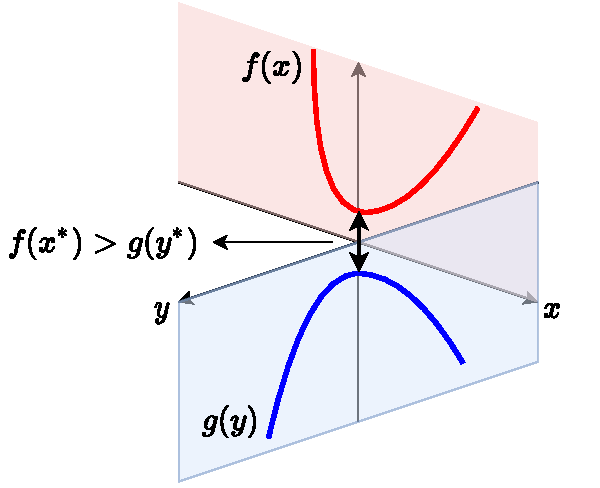
\includegraphics[width=\linewidth]{./figures/weak_dual.pdf}
      \captionsetup{justification=centering}
      \caption{Weak duality.}
    \end{subfigure}
    \hfill
    \begin{subfigure}{.48\textwidth}
      \centering
      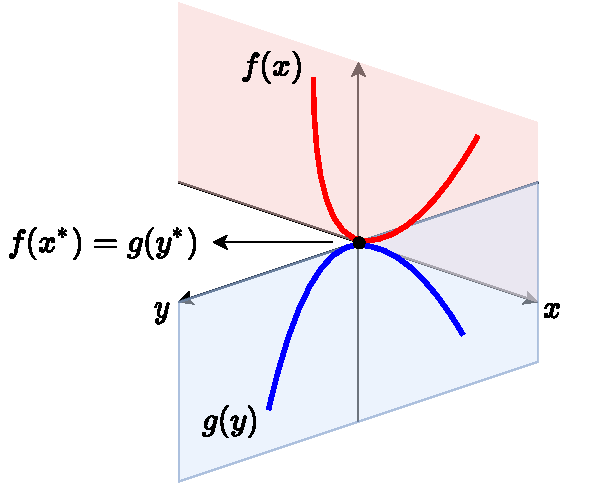
\includegraphics[width=\linewidth]{./figures/strong_dual.pdf}
      \captionsetup{justification=centering}
      \caption{Strong duality.}
    \end{subfigure}
    \captionsetup{justification=centering}
    \caption{Geometric illustration of weak and strong duality.}
    \label{fig:duality}
\end{figure}

\begin{theorem}[Duality theory~\protect{\citep[Theorem~11.39]{rockafellar1998variational}}] Consider the primal-dual pair:~\eqref{prob:general_primal} and~\eqref{prob:general_dual}, where $F: \Re^n \times \Re^m \to \Re$ is a proper, closed and convex function. The following properties hold. 
    \begin{itemize}
        \item \textbf{Weak duality}. The inequality $v_F(0) \geq v_F^{**}(0)$ always holds. 
        \item \textbf{Strong duality}. If $0 \in \ri\dom v_F \cup \ri\dom v_F^{**}$, then $v_F(0) = v_F^{**}(0)$. 
        \item \textbf{Optimal solutions.} If the strong duality holds with finite optimal values, then the following characterizations of the optimal solutions to the primal-dual pair are equivalent
            \begin{align}
                (x^*, 0) &\in \partial F^*(0,y^*); \\
                (0, y^*) &\in \partial F(x^*,0); \\
                v_F(0) = F^*(x^*, 0) &= -F^*(0,y^*) = v_F^{**}(0).
            \end{align}
    \end{itemize}
\end{theorem}

The perturbation function $F$ plays an important role in Fenchel-Rockafellar duality theory. Different choices of the perturbation function will lead to different dual problems. In the rest of this section, we will interpret three widely used primal-dual pairs: Lagrangian dual, Fenchel-Rockafellar dual and gauge dual, under this perturbation framework.  


\subsection{Lagrangian duality}
Consider the general constrained convex optimization problem:
\begin{equation} \label{prob:general_constrained} 
    \minimize{x \in \Re^n} f(x) \st c_i(x) \leq 0 \enspace \forall i = 1, \dots, m,
\end{equation}
where $f:\Re^n\to\Re$ and $c_i:\Re^n\to\Re$ for all $i\in[m]$ are convex functions. In this case, the perturbation function is defined as 
\begin{equation}
    F(x, u) = f(x) + \sum_{i = 1}^m \delta_{\leq 0}(c_i(x) + u_i).
\end{equation}
Then we can derive the corresponding conjugate function as 
\begin{align*}
    -F^*(0, y) &= -\sup_{x\in\Re^n, u\in\Re^m} \ip{0}{x} + \ip{y}{u} - F(x,u)
             \\&= -\sup_{x\in\Re^n, w\in\Re_+^m} \sum_{i=1}^m \ip{y_i}{- c_i(x) - w_i} - f(x)
             \\&= 
             \begin{cases}
                 \inf_{x\in\Re^n} f(x) + \sum_{i=1}^m \ip{y_i}{c_i(x)} & \text{if} y \in\Re_+^m \\
                 -\infty & \text{otherwise}.
             \end{cases}
\end{align*}
Therefore, the Lagrangian dual to problem~\eqref{prob:general_constrained} is given by
\begin{equation} \label{prob:general_constrained_dual}
    \maximize{y\in\Re_+^m} \minimize{x \in \Re^n} f(x) + \sum_{i=1}^m \ip{y_i}{c_i(x)}.
\end{equation}
The following theorem, summarized by \citet{boyd:2004}, characterizes the duality correspondence for the Lagrangian primal-dual pair. 

\begin{theorem}[Lagrangian duality theory~\protect{\citep[Section~5.3]{boyd:2004}}] 
    Let $p^*$ and $d^*$ denote respectively the optimal values for the Lagrangian primal-dual pair:~\eqref{prob:general_constrained} and~\eqref{prob:general_constrained_dual}. 
    \item \textbf{Weak duality}. $p^* \geq d^*$. 
    \item \textbf{Strong duality}. 
    If there exist an interior-point feasible point $\hat x$ for the primal problem~\eqref{prob:general_constrained}, i.e. $c_i(\hat x) < 0$ for $i = 1,\dots,m$, then $p^* = d^*$. Furthermore, let $x^*$ and $y^*$ denote respectively the optimal solutions to the primal-dual pair:~\eqref{prob:general_constrained} and~\eqref{prob:general_constrained_dual}, then 
    \[y_i^*c_i(x^*) = 0 \enspace \forall i = 1,\dots,m.\]
\end{theorem}


\subsection{Fenchel-Rockafellar duality}
Consider the following optimization problem 
\begin{equation} \label{prob:general_fenchel} 
    \minimize{x \in \Re^n} f(x) + g(Mx),
\end{equation}
where $f:\Re^n\to\Re$ and $g:\Re^m\to\Re$ are closed convex functions, and $M:\Re^n\to\Re^m$ is a linear operator. In this case, the perturbation function is defined as 
\begin{equation}
    F(x, u) = f(x) + g(Mx + u).
\end{equation}
Then we can derive the corresponding conjugate function as
\begin{align*}
    -F^*(0, y) &= -\sup_{x\in\Re^n, u\in\Re^m} \ip{0}{x} + \ip{y}{u} - f(x) - g(Mx + u)
             \\&= -\sup_{x\in\Re^n} \left\{\sup_{u\in\Re^m} \ip{y}{Mx + u} - g(Mx + u)\right\} - f(x) - \ip{y}{Mx}
             \\&= - g^*(y) - \sup_{x\in\Re^n}\ip{-M^*y}{x} - f(x) 
             \\&= - g^*(y) - f(-M^*y).
\end{align*}
Therefore, the Fenchel-Rockafellar dual to problem~\eqref{prob:general_fenchel} is given by
\begin{equation} \label{prob:general_fenchel_dual}
    \maximize{y\in\Re^m} - g^*(y) - f(-M^*y).
\end{equation}
The following theorem, developed by \citet{rockafellar1970convex}, characterizes the duality correspondence for the Fenchel-Rockafellar primal-dual pair. 

\begin{theorem}[Fenchel-Rockafellar duality theory~\protect{\citep[Corollary 31.2.1]{rockafellar1970convex}}] 
    Let $p^*$ and $d^*$ denote respectively the optimal values for the Fenchel-Rockafellar primal-dual pair:~\eqref{prob:general_fenchel} and~\eqref{prob:general_fenchel_dual}. 
    \item \textbf{Weak duality}. $p^* \geq d^*$. 
    \item \textbf{Strong duality}. 
    If $0\in\int(\dom g - M\dom f)$, then $p^* = d^*$. Furthermore, let $x^*$ and $y^*$ denote respectively the optimal solutions to the primal-dual pair:~\eqref{prob:general_fenchel} and~\eqref{prob:general_fenchel_dual}, then the following relationships hold
    \begin{align*}
          y^* &\in \partial g(Mx^*) \cap (M^*)^{-1}\partial f(x^*) \tand
        \\x^* &\in \partial f^*(-M^*y^*)\cap M^{-1}\partial g^*(y^*).
    \end{align*}
\end{theorem}




\subsection{Gauge duality}
Consider the following gauge optimization problem 
\begin{equation} \label{prob:general_gauge} 
    \minimize{x \in \Re^n} \gauge\Cs(x) \st Mx = b,
\end{equation}
where $\Cscr\subseteq\Re^n$ is a convex set and $\gauge\Cs$ is the corresponding gauge function, $M:\Re^n\to\Re^m$ is a linear operator, and $b\in\Re^m$ is a vector. By setting 
$\lambda \coloneqq 1/\gauge\Cs(x)$ and $w \coloneqq \lambda x$, problem~\eqref{prob:general_gauge} can be expressed as 
\begin{equation} \label{prob:general_gauge2} 
    \inf_{\lambda > 0, w \in \Re^n} \frac{1}{\lambda} \st w \in \Cscr \tand Mw = \lambda b.
\end{equation}
Note that minimizing $1/\lambda$ is equivalent to minimizing $-\lambda$ for $\lambda \geq 0$. In this case, the perturbation function is defined as 
\begin{equation}
    F(\lambda, w, u) = -\lambda + \delta\Cs(w) + \delta_{\{0\}}(\lambda b - Mw + u) + \delta_{\geq 0}(\lambda). 
\end{equation}
Then we can derive the corresponding conjugate function as
\begin{align*}
    -F^*(0, y) &= -\sup_{\lambda\in\Re, w\in\Re^n, u\in\Re^m} \ip{y}{u} + \lambda - \delta\Cs(w) - \delta_{\{0\}}(\lambda b - Mw + u) - \delta_{\geq 0}(\lambda)
    \\&= -\sup_{\lambda\in\Re, w\in\Re^n} \lambda - \delta\Cs(w) - \delta_{\geq 0}(\lambda) - \ip{\lambda b - Mw}{y}
    \\&= -\sup_{\lambda\geq 0} \delta\Cs^*(M^*y) + \lambda ( 1 - \ip{b}{y} )
    \\&= 
        \begin{cases}
            -\delta\Cs^*(M^*y) & \text{if} \ip{b}{y} \geq 1 \\
            -\infty & \text{otherwise}.
        \end{cases}
\end{align*}
Therefore, the gauge dual to problem~\eqref{prob:general_gauge} is given by
\begin{equation} \label{prob:general_gauge_dual}
    \maximize{y\in\Re^m} -\delta\Cs^*(M^*y) \st \ip{b}{y} \geq 1.
\end{equation}
The following theorem, developed by \citet{friedlander2014gauge}, characterizes the duality correspondence for the gauge primal-dual pair. 

\begin{theorem}[Gauge duality theory~\protect{\citep[Theorem~5.1 and Corollary~5.2]{friedlander2014gauge}}] 
    Let $p^*$ and $d^*$ denote respectively the optimal values for the gauge primal-dual pair:~\eqref{prob:general_gauge} and~\eqref{prob:general_gauge_dual}. 
    \item \textbf{Weak duality}. If both primal problem~\eqref{prob:general_gauge} and dual problem~\eqref{prob:general_gauge_dual} are feasible, then $p^* d^* \geq 1$. 
    \item \textbf{Strong duality}. If either primal problem~\eqref{prob:general_gauge} or dual problem~\eqref{prob:general_gauge_dual} is strictly feasible and the other is feasible, then $p^* d^* = 1$. Furthermore, let $x^*$ and $y^*$ denote respectively the optimal solutions to the primal-dual pair:~\eqref{prob:general_gauge} and~\eqref{prob:general_gauge_dual}, then 
    \[\ip{x^*}{M^*y^*} = \gauge\Cs(x^*)\delta\Cs^*(M^*y^*).\]
    
\end{theorem}

\section{Structured optimization} \label{sec:1-3}

Convex optimization provides a valuable computational framework that renders many problems tractable because of the range of powerful algorithms that can be brought to the task. The key is that a specific mathematical structure, i.e., the convexity of the functions and sets defining the problem—opens an enormous range of theoretical and algorithmic tools that lend themselves astonishingly well to computation. However, there are limits to the scalability of general-purpose algorithms for convex optimization. As has been recognized in the optimization and related communities for at least the past decade, significant efficiencies can be gained by acknowledging the latent structure in the solution itself, coupled with the overarching structure provided by convexity.

Structured optimization proceeds by using a prescribed set of atoms to assemble an optimal solution. The atomic decomposition of a vector $x\in\Re^n$ with respect to an atomic set
$\Ascr\subset\Re^n$ is given by the weighted superposition
\begin{equation} \label{eq:atomic-decomp}
  x = \sum_{a\in\Ascr} c_a a, \quad c_a\ge0 \quad \forall a\in\Ascr.
\end{equation}
Each coefficient $c_a$ in the atomic decomposition measures the contribution of
the corresponding atom $a$ toward the representation of $x$. Intuitively, an
atomic decomposition reveals structural information implicit in a vector, with
large coefficients in the decomposition indicating the more essential
structures.

Within the context of an optimization problem, the atomic decomposition reveals
structural elements most essential in the minimization process.
In the simplest case, the atoms $\Ascr$ may be formed from the collection of
signed canonical unit vectors $\{\pm e_1,\ldots,\pm e_n\}$, which leads to the
atomic decomposition
\[
  x = \sum_{j=1}^n c_j a_j,
  \quad
  c_j: = |x_j|,
  \quad
  a_j:= (\sgn x_j)\cdot e_j.
\]
Trivially, the essential atoms thus correspond to the variables $x_j$ in
the vector $x=(x_1,\ldots,x_n)$ with nonzero magnitude.

This generic model for atomic decompositions was promoted by~\citet{cds98} in the context of sparse signal decomposition, and more recently, by~\citet{chandrasekaran2012convex}, who were concerned with obtaining sparse solutions to linear inverse problems. 

In this thesis, we want to answer the question of determining which of the atoms in the atomic set $\Ascr$ are essential to the atomic decomposition of $x$, and conversely, which atoms can be safely ignored. In \autoref{ch:Dual-Struc-Opt}, we study the atomic decomposition framework from a dual perspective. Polarity, which extends the familiar notion of orthogonality from linear sets to general convex sets, plays a special role in a simple and geometric form of convex duality. This duality correspondence yields a general notion of alignment that leads to an intuitive and complete description of how atoms participate in the final decomposition of the solution. The resulting dual perspective leads to variations of existing algorithms effective for large-scale problems. We illustrate these ideas with many examples, including applications in matrix completion and morphological component analysis. We further show that this dual alignment property allows us to design new structured optimization models for real-world applications and develop efficient and scalable algorithms for structured optimization problems. We briefly introduce the roadmap below. 

In \autoref{ch:App-Sig-Demix}, we study the structured signal demixing problem which seeks to separate a superposition of multiple signals into its constituent structural components. We propose a two-stage approach that first decompresses and subsequently deconvolves the noisy and undersampled observations of the superposition. Probabilistic error bounds are given on the accuracy with which this process approximates the individual signals. The theory of polar convolution of convex sets developed by~\citet{friedlander2019polarconvolution}, and the dual alignment property developed in \autoref{ch:Dual-Struc-Opt} play central roles in the analysis and solution process. If the measurements are random and the noise is bounded, this approach stably recovers low-complexity and mutually incoherent signals, with high probability and with optimal sample complexity. Numerical experiments on both real and synthetic data confirm the theory and the efficiency of the approach.

In \autoref{ch:App-Primal-Retrieval}, we study the structured data-fitting problem, which is prevalent in machine learning and data mining. In practice, people solve the corresponding structured convex relaxations. When tackling high-dimensional structured optimization problems, dual-based algorithms are usually preferred over primal-based algorithms as dual variables usually live in a much lower-dimensional space than primal variables. One common issue of dual-based algorithms is that they still need to translate dual variables to primal variables at some point. How to retrieve a near-optimal primal variable efficiently with a provable guarantee is thus crucial for the success of dual approaches. We present a simple and computationally cheap strategy for retrieving a primal variable from any feasible dual variable, which is based on the dual alignment property developed in \autoref{ch:Dual-Struc-Opt}. Theoretically, we show that our proposed strategy is capable of obtaining a near-optimal primal variable given a dual-based algorithm converging to the optimal dual solution. Numerical experiments on real-world datasets support our analysis.

In \autoref{ch:App-AtomicOpt}, we introduce our open-source package \texttt{AtomicOpt.jl} for solving a class of structured optimization problems, which is written in the Julia programming language~\citep{bezanson2017julia}. Our design depends on the level-set method~\citep{aravkin2016levelset}, a dual version of the conditional-gradient method~\cite{jaggi2013revisiting,frank1956algorithm,dunn1978conditional}, and the primal-retrieval strategy developed in~\autoref{ch:App-Primal-Retrieval}. The worst-case computational complexity of our algorithm is sublinear in the required accuracy. All the numerical experiments conducted in~\autoref{ch:Dual-Struc-Opt},~\autoref{ch:App-Sig-Demix} and~\autoref{ch:App-Primal-Retrieval} are reproducible via this package. 



 

\section{Federated learning} \label{sec:1-4}

With the development of artificial intelligence, people recognize that many powerful machine learning models are driven by large decentralized datasets, e.g., AlphaGo~\citep{silver2016mastering} and AlexNet~\citep{krizhevsky2012imagenet}. In many industry-scale applications, training data is distributed in the form of silos, that is, training data is obtained and maintained by many data owners instead of being centralized at the place of a single owner or a data center. Because of industrial competition, privacy concerns, legal restrictions, and many other possible reasons, integrating or centralizing data from different sources faces enormous resistance and is often even infeasible~\citep{li2020review}. Federated learning, originally proposed by~\citet{federated2016}, is promising for training machine learning models on distributed data sources. It facilitates collaboration among a group of data owners (aka.~``clients'') and, at the same time, preserves their privacy. The central idea of federated learning is to periodically aggregate local models from clients to produce a more general and capable global model.

Federated learning can be further be classified into two main categories: horizontal federated learning and vertical federated learning~\cite{yang2019federated}. Horizontal federated learning refers to the scenarios where various clients' data sets share the same feature space but have separate sample IDs, and vertical federated learning refers to the scenarios where data sets owned by different clients share the identical sample IDs but have distinctive features. A simple characterization is shown in \autoref{fig:hfl_and_vfl}. 

\begin{figure}[t] 
    \begin{subfigure}{.48\textwidth}
      \centering
      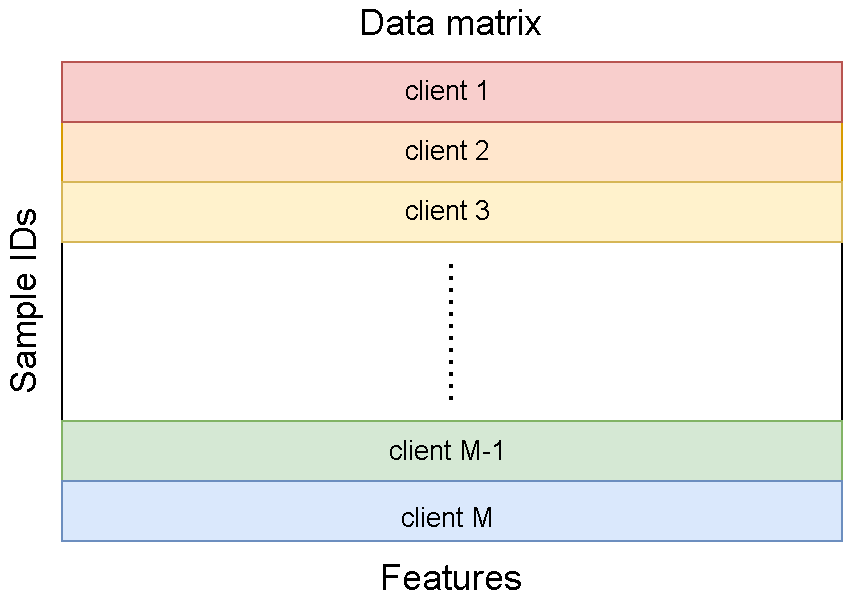
\includegraphics[width=\linewidth]{./figures/hfl_illustration.pdf}
      \captionsetup{justification=centering}
      \caption{Horizontal federated learning.}
      \label{fig:hfl}
    \end{subfigure}
    \hfill
    \begin{subfigure}{.48\textwidth}
      \centering
      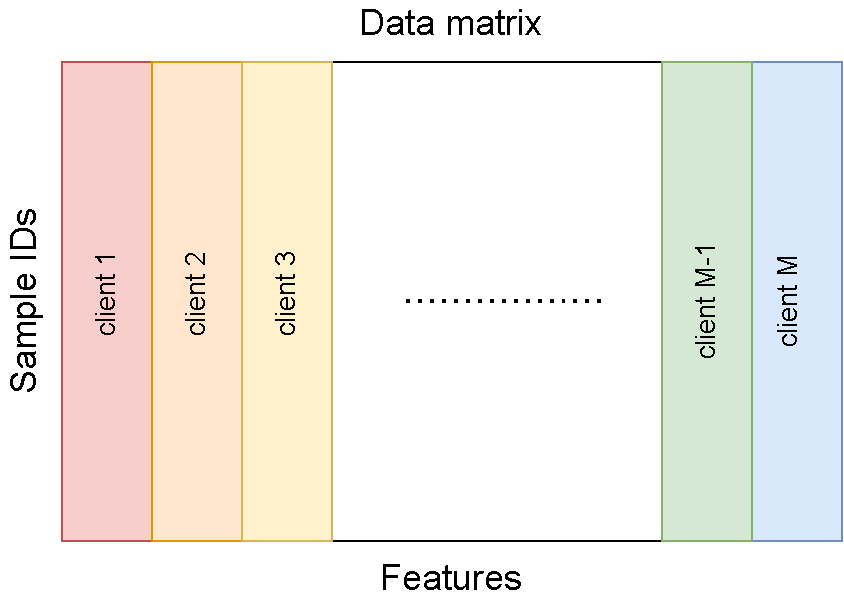
\includegraphics[width=\linewidth]{./figures/vfl_illustration.pdf}
      \captionsetup{justification=centering}
      \caption{Vertical federated learning.}
      \label{fig:vfl}
    \end{subfigure}
    \captionsetup{justification=centering}
    \caption{Characterization of horizontal and vertical federated learning.}
    \label{fig:hfl_and_vfl}
\end{figure}

This thesis shows that duality can be utilized to develop efficient and scalable algorithms for the optimization problem arising from federated learning. Besides, we show that structured optimization techniques can play an essential role in designing fair contribution valuation rules in federated learning. We briefly introduce the roadmap below. 

\subsection{Federated optimization} \label{sec:1-4-1}

A federated learning system is often composed of two components: clients and a central server at the physical level. The learning process in federated learning can be formulated as a distributed optimization problem, also known as federated optimization. As characterized and formalized by~\citet{wang2021field},~\citet{li2020federated} and~\citet{li2019convergence}, several essential characteristics distinguish FO from standard machine learning and distributed optimization. 

\begin{assumption}[Governing assumptions for federated optimization] \label{assum:govern}
The following assumptions hold for federated optimization. 
  \begin{itemize}
    \item \textbf{Slow Communication.}  Communication between clients and a central server is assumed to be the main bottleneck and dominates any computational work done at each of the clients. 
    \item \textbf{Data Privacy.} Clients want to keep their local data private, i.e., their data can not be accessed by any other client nor by the central server.
    \item \textbf{Data heterogeneity.} The training data are not independent and identically distributed (i.i.d.). In other words, a client’s local data cannot be regarded as samples drawn from single overall distribution.
    \item \textbf{Partial Participation.} Unlike traditional distributed learning systems, an FL system does not have control over individual client devices, and clients may have limited availability for connection. 
\end{itemize}
\end{assumption}

In \autoref{ch:Dual-Fed-Opt}, we study the federated optimization problem from a dual perspective. We propose a new algorithm termed federated dual coordinate descent (FedDCD), which is based on a type of coordinate descent method developed by \citet{necoara2017random}.  Additionally, we
enhance the FedDCD method with inexact gradient oracles and Nesterov's acceleration. We demonstrate
theoretically that our proposed approach achieves better convergence rates than the state-of-the-art
primal federated optimization algorithms under certain situations. Numerical experiments on real-world
datasets support our analysis.

\subsection{Contribution valuation in federated learning} \label{sec:1-4-2}

The effectiveness of federated learning depends on the active participation of motivated clients. Another important question in federated learning is how to ensure the clients’ long-term engagement, and how to motivate more clients' participation. One possible practical solution is to recompense the participated clients according to their contribution. 

Shapley value~\cite{shapley201617} is a classical measure originates from cooperative game theory to fairly assess contributions by participants in a coalition. 
The Shapley value of a participant is defined as the expectation of the marginal contribution of the participant over all possible subsets of the other participants. Shapley value is the unique measure that satisfies the four fundamental requirements of fairness proposed by Shapley~\cite{shapley201617}: balance, symmetry, zero element and additivity, which we formally define bellow. 

\begin{definition} \label{def:shapley}
    Supporse there are $M$ clients and there is a black-box utility function $U:2^{[M]} \to \Re$ such that for any subset of clients $S \subseteq [M]$, the function $U(S)$ returns a utility score of the model collaboratively trained by the clients in $S$, such as the performance of the model. Let $v: [M] \to \mathbb{R}$ be the evaluation metric associated with the utility function $U$. The metric $v$ is called \emph{Shapley-fair} with respect to $U$ if it satisfies the following for fundamental requirements
    \begin{enumerate}
        \item \textbf{Symmetry.} For any two clients $i, j \in [M]$, if for any subset of clients $S \subseteq [M] \setminus \{i,j\}$, $U(S \cup \{i\}) = U(S \cup \{j\})$, then $v(i) = v(j)$. 
        \item \textbf{Zero element.} For any client $i \in [N]$, if for any subset of clients $S \subseteq [M] \setminus \{i\}$, $U(S \cup \{i\}) = U(S)$, then $v(i) = 0$.
        \item \textbf{Additivity.} If the utility function $U$ can be expressed as the sum of separate utility functions, namely $U = U_1 + U_2$ for some $U_1, U_2 : 2^I \to \mathbb{R}$, then for any client $i \in [M]$, $v(i) = v_1(i) + v_2(i)$, where $v_i$ and $v_2$ are the evaluation metrics associated with the utility functions $U_1$ and $U_2$, respectively. 
        \item \textbf{Balance.}  $U([M]) = \sum_{i \in [M]} v(i)$.
    \end{enumerate}
\end{definition}

Under the federated learning setting, a utility function is usually defined as the model performance on a data set. The symmetry requires that the same contributions to the performance should receive the same evaluation, which implies that clients with same local data sets should receive same evaluation. The zero element requires that no contribution, no value is recognized. The additivity requires that if there are multiple tasks and thus multiple test data sets, then the contributions of any client with respect to the test data sets can be expressed as the sum of the contributions with respect to those different tasks and test data sets. Note that, although balance is a necessary condition in many economic contests because it ensures payment is fully distributed to all clients, it is irrelevant in the context of federated learning because we are only concerned about the relative contributions of clients. It is shown~\cite{dubey1975uniqueness,ghorbani2019data} that if the data valuation metric $v$ satisfies symmetry, zero element, and additivity, then $v$ must have the form
\begin{equation} \label{eq:shapley}
    v(i) = c \sum\limits_{S \subseteq I \setminus\{i\}} \frac{1}{\binom{N-1}{|S|}} \left[U(S\cup\{i\}) - U(S)\right],
\end{equation}
for some positive constant $c$.  

Although Shapley value has many desirable properties, evaluating Shapley value in federated learning requires exhaustive retraining and evaluating the model on every subset of clients. The costs of communication and time may be prohibitive in practice~\cite{song2019profit}. To tackle this challenge, some variations inspired by Shapley value were developed. Federated Shapley value (FedSV), recently proposed by \citet{wang2020principled}, is a measure for valuating contribution under the framework of horizontal federated learning. The key idea is to compute the Shapley values for clients in each round of training and then report the summation over all the rounds as the final results. This design cleverly avoids model retraining. However, there are still factors of potential unfairness in the design of FedSV because two data owners with the same local data may not receive the same evaluation. 

In \autoref{ch:Val-HFL}, we propose a new measure called completed federated Shapley value (ComFedSV) for contribution valuation in horizontal federated learning, which improves the fairness of FedSV. The design depends on completing a matrix consisting of all the possible contributions by different subsets of the data owners. It is shown under mild conditions that this matrix is approximately low-rank by leveraging concepts and tools from structured optimization. Both theoretical analysis and empirical evaluation verify that the proposed measure does improve fairness in many circumstances.

In \autoref{ch:Val-VFL}, we extend the idea of FedSV to vertical federated learning. We propose a contribution valuation metric called vertical federated Shapley value (VerFedSV), which utilizes tools from structured optimization. We show that VerFedSV not only satisfies many desirable properties for fairness but is also efficient to compute, and can be adapted to both synchronous and asynchronous vertical federated learning algorithms. Both theoretical analysis and extensive experimental results verify the fairness, efficiency, and adaptability of VerFedSV.






\part{Structured optimization}

%    2. Duality in structured optimization
%% The following is a directive for TeXShop to indicate the main file
%%!TEX root = diss.tex
\chapter{Duality in structured optimization}
\label{ch:Dual-Struc-Opt}

\section{Background}
As we introduced in \autoref{sec:struc-opt}, structured optimization uses a prescribed set of atoms to assemble a solution that fits a model to data. Our purpose with this chapter is to describe the rich convex geometry and the duality that
underlies atomic decomposition. The path we follow builds on the duality
inherent in convex cones: every convex cone is paired uniquely with another cone that is polar to it. The extreme rays of each cone in this pair are in some sense \emph{aligned}. Brought into the context of atomic decomposition, this
notion of alignment through the polar operation provides a theoretical framework
that can be harnessed to identify the atoms that participate in a decomposition. This
approach facilitates certain algorithmic design patterns that promote
computational efficiency, as we demonstrate with concrete examples. Similar
computational economies accrue within reduced-space active-set methods for
optimization problems with inequality constraints, such as implemented by the
MINOS software package \citep{murtsaun:1983}.

Early work in structured optimization focused on problem formulations meant to
produce sparse solution vectors, i.e., a solution with relatively few non-zero
elements. Compressed sensing \cite{cds98,chendonosaun:2001,crt06a} and model
selection \cite{tibshirani1996regression,tibshirani1997lasso} , with their many applications
in signal processing and statistics, helped to establish sparse optimization as
an important class of problems with a range of specialized algorithms.
Generalizations that accommodated different notions of sparsity soon followed,
including matrix problems with low-rank solutions (sparsity in the vector of
singular values), fused index pairs (sparsity in terms of the norms of subgroups of variables), and sparsity in specialized dictionaries, such as mass
spectrographs of simple molecules used to represent structures of
more complicated molecules \cite[Section~6.3.1]{vandenberghe:2010}.

Nonsmooth regularization functions that promote sparsity, such as the 1-norm for
sparse vectors, or the nuclear norm for low-rank matrices, are key features of
these formulations. Gauge functions, which significantly generalize the notion
of a norm, were recognized as flexible regularization functions that promote a
broad range of sparse structures. By defining a set of atoms from which to build
a solution, an almost arbitrary set of solution structures can be considered.
The gauge function to this set can be incorporated into a convex optimization
problem in order to obtain a solution with the desired structure. The convex
analysis of gauges and support functions, which are their dual counterparts, is
rich in geometry and rife with opportunity for efficient algorithm
implementations for high-dimensional problems. Our purpose with this monograph
is to expose the basic elements of this theory and its many connections to
sparse and structured optimization. To make it accessible researchers who are
not specialists in convex analysis, we chose a largely self-contained treatment
and make a few modest assumptions that greatly simplify the derivations.

\subsection{Applications and prior work}

One of the main implications of our approach is its usefulness in using dual
optimization methods for discovering atomic decompositions. With the tools of
polar alignment, a dual optimization method can be interpreted as solving for an
aligning dual vector $z$ that exposes the support of a primal solution $x$. If
the number of exposed atoms is small, a solution $x$ of the primal problem can
be obtained from a reduced problem defined over the exposed support, but without
the nonsmooth atomic regularization. The resulting reduced problem is often
computationally much cheaper~\citep{freund2017extended} and better
conditioned~\citep{negahban2012restricted}. Alternatively, two-metric methods can
be designed to act differently on a primal iterate's suspected
support~\citep{gafni1984two}. In many applications, such as feature selection,
knowing the optimal support may itself be sufficient.  As we illustrate through
various examples, there are several important cases where the dual aligning
vector $z$ can be computed directly.

\paragraph{Machine learning}

The regularized optimization problems described in \autoref{sec:manifestations}
frequently appear in applications of machine learning for the purpose of model
complexity reduction. The most popular tools are the vector 1-norm in feature
selection~\cite{tibshirani1996regression}, its group-norm
variant~\cite{jacob2009group}, and the nuclear norm in matrix completion
\cite{recht2010guaranteed}. 
Many other sparsity-promoting regularizers, however,
appear in practice \cite{zeng2014ordered}. Although unconstrained formulations
are most popular, particularly when the proximal operator is computationally
convenient~\cite{parikh2013proximal}, the gauge-constrained formulation is
frequently used and solved via the conditional gradient method
\cite{frank1956algorithm,dunn1978conditional,jaggi2013revisiting}. Popular dual
methods, which iterate over a dual variable $z^{(k)}$ but maintain the
corresponding primal variable $x^{(k)}$ only implicitly, include bundle methods
\cite{lemarechal1981bundle} and dual averaging
\citep{xiao2010dual,duchi2012dual}.

\paragraph{Linear conic optimization}

Conic programs are a cornerstone of convex optimization. The nonnegative cone,
the second-order cone and the semidefinite cone respectively, give rise to
linear, second-order, and semidefinite programs. These problem classes capture
an enormous range of important models, and can be solved efficiently by a
variety of algorithms, including interior methods
\cite{karmarkar1984new,nen94,rene:2001}. Conic programs and their associated
solvers are key ingredients for general purpose optimization software packages
such as YALMIP~\citep{lofberg2004yalmip} and CVX~\cite{grant2008cvx}. The
alignment conditions for these specific cones have been exploited in dual
methods, such as in the spectral bundle method for large-scale semidefinite
programming \cite{helmberg2000spectral}. \autoref{example-conic-opt} demonstrates
this alignment principle in the context of conic optimization.

\paragraph{Gauge optimization} 

The class of gauge optimization problems, as defined by Freund's 1987 seminal
work~\citep{freund1987dual}, can be simply stated: find the element of a convex
set that is minimal with respect to a gauge function. These conceptually simple
problems appear in a remarkable array of applications, and include parts of
sparse optimization and all of conic
optimization~\cite[Example~1.3]{friedlander2014gauge}. This class of
optimization problems admits a duality relationship different from classical
Lagrange duality, and is founded on the polar inequality.
In this context, the polar inequality provides an analogue to weak duality,
well-known in Lagrange duality, which guarantees that any
feasible primal value provides an upper bound for any feasible dual
value. In the gauge optimization context, a primal-dual pair $(x,z)$ is optimal
if and only if the polar inequality holds as an equation, which under
\autoref{def:alignment} implies that $x$ and $z$ are
aligned. 
The connection between polar alignment and optimality is
discussed further in \autoref{sec:gauge-optimization}.

\paragraph{Two-stage methods}
In sparse optimization, two-stage methods first identify the primal variable
support, and then solve the problem over a reduced support
\cite{ko1994iterative,cristofari2017two}. If the support is sparse enough, the
second problem may be computationally much cheaper, either because it allows for
faster Newton-like methods, or because of better conditioning
\cite{negahban2012restricted}. The atomic alignment principles we describe in
\autoref{sec:convexanalysis-atomic} give a general recipe for extracting primal
variable support from a computed dual variable, which at optimality is aligned
with the primal variable; see \autoref{sec:manifestations}. 

\paragraph{Method interpretability}
The connection between sparsity and alignment points to a likely ``aligning
behavior" in many of the most effective methods for sparse
optimization~\cite{hare2004identifying}. Indeed, we show in \autoref{sec:methods}
that this is true for a range of methods, including proximal gradient,
conditional gradient, and cutting plane methods. Surprisingly, we also find
hints of aligning behavior in seemingly unrelated methods, such as augmented
Lagrangian and bundle methods. The alignment point of view thus offers greater
interpretability of commonly used methods in many modern optimization
applications.

\section{Atomic decomposition} \label{sec:atomic-decomposition}
Recall the atomic decomposition of a vector $x\in\Re^n$ with respect to an atomic set $\Ascr\subseteq\Re^n$; see \eqref{eq:atomic-decomp}. We are particularly interested in the question of determining which of the atoms
in $\Ascr$ are essential to the atomic decomposition of $x$, and conversely,
which atoms can be safely ignored. 

\subsection{Gauge functions reveal the atomic support}
The following equivalent expression of the gauge function 
\begin{equation}
    \label{eq:gauge2}
    \gauge\As(x)
    = \inf_{c_a}
      \left\{ \sum_{a\in\Ascr}c_a ~\bigg\vert~ x = \sum_{a\in\Ascr}c_aa,\ c_a \ge0\ \forall a\in\Ascr \right\},
\end{equation}
helps to define the answer to the question above; cf.~\autoref{prop-guage-equivalence}. This function returns the
minimal sum of weights over all valid atomic decompositions of $x$ with respect
to the set $\Ascr$. The value $\gauge\As(x)=\infty$ indicates that there doesn't
exist a valid atomic decomposition for $x$. (For example, an atomic set composed
of nonnegative vectors cannot decompose a vector~$x$ that contains negative entries.) 

In the framework outlined by \citet{chandrasekaran2012convex}, the gauge
function $\gauge\As$ defines the objective of a convex optimization problem
suitable for recovering a signal from a small number of partial observations. In
that context, the number of atoms needed to decompose the signal determines the
number of observations needed to reconstruct the signal.

The significant atoms---those that \emph{support} the
vector $x$---are those that contribute positively in forming the minimal sum. We
are thus led to the following definition.

\begin{definition}[Atomic support] \label{def:support} A subset of atoms
    $\suppa(x)\subset\Ascr$ is a \emph{support set} for $x$ with respect to
    $\Ascr$ if every atom $a\in\suppa(x)$ has a strictly positive coefficient
    $c_a$ in the atomic decomposition~\eqref{eq:atomic-decomp}. That is,
    \begin{equation}
      \label{eq:support}
      \gauge\As(x) = \sum_{\mathclap{a\in\suppa(x)}} c_a,
      \qquad x = \sum_{\mathclap{a\in\suppa(x)}} c_aa,
      \text{and} c_a > 0\enspace \forall a\in\suppa(x).
    \end{equation}
    The set $\supp\As(x)$ is defined as the set of all support
    sets. Thus, any set in $\supp\As(x)$ is a valid support set. 
  \end{definition}

\subsection{Polar inequality} \label{sec:approach}

How do we identify the support of a vector $x$ with respect to an arbitrary
atomic set $\Ascr$? The direct approach requires us to solve the minimum-weight
problem defined by the gauge~\eqref{eq:gauge2}, and determine a valid decomposition
from the positive elements of the computed solution. Thus, to identify all
possible atomic support sets, we need to compute all possible solutions
to~\eqref{eq:gauge2}. As we will demonstrate, however, a complete description of all
possible solution sets can be obtained using the concept of \emph{polar
alignment}, which we define in this section. Our approach is based on a certain
duality correspondence particular to gauge functions and to convex cones that
are implicit in their definition. We describe in \autoref{sec:convexanalysis} this correspondence and its relationship to atomic decompositions. Here we give only the basic elements needed to define the notion of alignment. The next proposition shows the close relationship between the gauge function and the support function. 

\begin{proposition}[Polar inequality] \label{prop:polar-inequality}
    For all pairs of vectors $(x,z)\in\dom\gauge\As\times\dom\sigma\As$,
    \begin{equation}
      \label{eq:polar-inequality}
      \ip x z \le \gauge\As(x)\cdot\sigma\As(z).
    \end{equation}
\end{proposition}

\begin{figure}[t] 
    \centering
    \includegraphics[page=10]{./figures/illustrations.pdf}
    \caption{%
    An illustration of the proof of the polar
    inequality given by \autoref{prop:polar-inequality}. The inner-product of the scaled vector $\hat x = x/\gauge\As(x)$ with $z$ always lies in the left halfspace defined by
    $\sigma\As(z)$, i.e., $\ip{\hat x}{z}\leq\sigma\As(z)$.
    }
    \label{fig:polar-inequality}
\end{figure}

\begin{proof}
    The proof for the polar inequality in
    \cite[Section~15]{rockafellar1970convex} relies on the polarity of cones.
    Here we provide an elementary proof that only depends on the provided
    definitions of gauge and support functions. First, consider the case
    $\gauge\As(x) > 0$. Let $\xhat=x/\gauge\As(x)$. Thus, $\xhat\in\convA$, and
    \[
      \ip{x}{z} = \gauge\As(x)\cdot\ip{\xhat}{z} \leq \gauge\As(x)\cdot\sigma\As(z),
    \]
    where the inequality follows from the maximality property of the support
  function; see \autoref{fig:polar-inequality}. Next, consider the case $\gauge\As(x)
  = 0$, and proceed by contradiction. Suppose $\ip{x}{z} > 0$. Because
  $\gauge\As(x) = 0$ implies $\lambda x \in \convA$ for all $\lambda > 0$, it
  follows from the positive homogeneity of $\sigma\As$ that $\sigma\As(z) =
  \infty$. This contradicts the assumption that $z \in \dom\sigma\As$. Thus, 
  \[
     \ip{x}{z} \leq 0 = \gauge\As(x)\cdot\sigma\As(z).
  \]
\end{proof}

\begin{example}[Norms] \label{ex:norms}
    When $\Ascr=\{x|\|x\|\le1\}$ is the unit level set to any norm,
  $\|\cdot\|:\Real^n\to\Real_+$, then
  \[
    \gauge\As(x) = \|x\|
    \text{and}
    \sigma\As(z) = \|z\|_d,
  \]
  where $\|\cdot\|_d$ is the dual norm. The polar inequality then reduces to the
  standard inequality between inner products and dual pairs of norms:
  \[
    \ip x z \le \|x\|\cdot \|z\|_d. 
  \]
\end{example}

\subsection{Alignment and support identification}

The polar inequality motivates the following generalized definition of aligned
pairs of vectors.
\begin{definition}[Alignment] \label{def:alignment} A pair
  $(x,z)\in\Real^n\times\Real^n$ is \emph{aligned} with respect to the atomic
  set $\Ascr$, i.e., $x$ and $z$ are $\Ascr$-aligned, if the polar
  inequality~\eqref{eq:polar-inequality} holds as an equation.
\end{definition}

This general notion of alignment follows from the special case where
$\Ascr=\{x|\norm{x}_2 \leq 1\}$ is the unit 2-norm ball. In this case, it follows
from \autoref{ex:norms} that the polar inequality reduces the Cauchy-Schwartz inequality
\begin{equation*}
  \label{eq:cauchy-inequality}
  \ip x z \le \norm{x}_2\cdot\norm{z}_2.
\end{equation*}
This inequality holds as an equation if and only if $x$ and $z$ are aligned in
the usual sense: there exists a nonnegative scalar $\alpha$ such that
$x=\alpha z$. The more general notion of alignment captures other important special
cases, including the H\"older inequality, which is a
special case of~\eqref{eq:polar-inequality} in which $\Ascr$ is the unit
$p$-norm ball, with $p\in[1,\infty]$.

A rich convex geometry underlies this general notion of alignment, and plays a
role in identifying the atoms important for the decomposition~\eqref{eq:atomic-decomp}.
Suppose that a vector $z$ is $\Ascr$-aligned with $x$. As we demonstrate
in \autoref{prop:support-identification}, all atoms $a\in\Ascr$ in the atomic support 
of $x$ must also be $\Ascr$-aligned with $z$, i.e.,
\begin{equation} \label{eq:exposed-atoms}
  \suppa(x)\subseteq\Escr\As(z):=\{a\in\Ascr\cup\{0\} | \ip a z = \sigma\As(z) \}.
\end{equation}
To see that $\Escr\As(z)$ indeed contains all the atoms that are $\Ascr$-aligned
with $z$, note that any atom $a\in\Escr\As(z)$ necessarily has unit gauge value,
i.e., $\gauge\As(a)=1$, which follows from 
\autoref{prop:polar-inequality}. Thus the condition $\ip a z = \sigma\As(z)$
implies that $a$ is $\Ascr$-aligned with $z$. \autoref{fig:essential-atoms}
presents a visualization of this concept. The atoms in $\Escr\As(z)$ are said to
be \emph{exposed} by the vector $z$. As we show in \autoref{sec:exposed-faces},
this set of atoms is contained in the face of $\convA$ exposed by the vector
$z$.

\begin{figure}[t]
    \centering
    \includegraphics[page=4]{./figures/illustrations}
    \caption{The set of atoms in the set $\Ascr$ generally (but not necessarily)
      defines the boundary of the convex hull $\convA$. The set of exposed atoms
      $\Escr\As(z)$ are contained within the supporting hyperplane $\{a|\ip{a}{z}
      =\sigma\As(z)\}$ normal to $z$. The atom $a_1$ is exposed by $z_1$ and all
      other directions that lie in the shaded cone; the atom $a_2$ is exposed by
      the unique direction along $z_2$; and the set of atoms
      $\{a_{3i}\}_{i=1}^3$ are exposed by the unique direction along $z_3$. }
    \label{fig:essential-atoms}
 \end{figure}


\subsection{Examples}

There are many varieties of atomic sets and recognizable convex
regularizers used to obtain sparse decompositions.
\citet{chandrasekaran2012convex} and
\citet{jaggi2013revisiting} both give extensive lists of atoms
and the norms that they induce, as well as their applications in practice.
Here we provide several simple examples that illustrate the variety of
ways in which vectors can be aligned.

\begin{example}[One norm] \label{example-one-norm} Let
    \[\Ascr = \{\pm e_1,\ldots,\pm e_n\}\] be the signed standard basis vectors.
    The gauge to this atomic set induces the 1-norm, which is the canonical
    example of a sparsifying convex penalty. The corresponding support function is
    the dual $\infty$-norm:
    \[
      \gauge\As(x) = \|x\|_1 \text{and} \sigma\As(z) = \|z\|_\infty.
    \]
    The polar inequality~\eqref{eq:polar-inequality} reduces to
    H\"older's inequality for these norms---i.e.,
    $\ip x z \le \|x\|_1\cdot\|z\|_\infty$. As is well known, this holds
    with equality---and thus $x$ and $z$ are $\Ascr$-aligned---if and only
    if
  \begin{equation*}
    x_i \neq 0
    \quad\Longrightarrow\quad
    \sgn(x_i) z_i = \max_j\,|z_j| \quad \forall i=1:n.
  \end{equation*}
  Alignment of the pair $(x,z)$ with respect to the atomic set $\Ascr$ is hence
  equivalent to the statement that $\suppa(x)\subseteq\Escr_\Ascr(z)$, where the
  atomic support for $x$ and the atoms exposed by $z$, respectively, are given the
  the sets
  \begin{align*}
    \suppa(x) &= \{\sgn(x_i)\cdot e_i | x_i \neq 0\},
  \\\Escr_\Ascr(z) &= \{\sgn(z_i)\cdot e_i | |z_i| =  \max_j\,|z_j| \}.
  \end{align*}
  
  The inclusion $\suppa(x)\subseteq\Escr_\Ascr(z)$ also characterizes an
  optimality condition. For example, consider the LASSO~\cite{tibshirani1997lasso}
  problem
  \begin{equation*}
    \minimize{x}\enspace \half\|Ax-b\|_2^2 \enspace\st\enspace\|x\|_1\le\tau,
  \end{equation*}
  where $\tau$ is a positive parameter. It's straightforward to verify that
  $x$ is optimal for this problem if and only if
  $\suppa(x)\subseteq\Escr_\Ascr(z)$ where $z:=A\T(b-Ax)$ is the negative gradient
  of the objective. \autoref{sec:manifestations} describes in detail the
  connection between optimality and alignment.
  \end{example}

  \begin{example}[Nuclear norm] \label{example-nuclear-norm}

    The nuclear norm, or Schatten 1-norm, of a matrix is the spectral analog to
    the vector 1-norm. The nuclear norm and its dual spectral norm can be obtained
    via the atomic set 
    \[
      \Ascr = \{uv^T | \|u\|_2=\|v\|_2 = 1\}
    \]
    of normalized $n$-by-$m$ rank-1 matrices. Let $X$ and $Z$ both be $m$-by-$n$
    matrices with singular values $c_1\ge\cdots\ge c_{m\wedge n}\ge0$ and
    $s_1\ge\cdots\ge s_{m\wedge n}\ge0$, where $m\wedge n:=\min\{m,\, n\}$. The
    corresponding gauge for $X$ is the nuclear norm
    \[
      \gauge\As(X) = \|X\|_1 := \sum_{i=1}^{m\wedge n}c_i,
    \]
    and the support function for $Z$ is the Schatten 2-norm
    \[
       \sigma\As(Z) = \|Z\|_\infty:=\max_{i=1:m\wedge n}s_i.
    \]
    The atomic description of these functions is consistent with the notion that
    the nuclear norm is a convex function that promotes low rank (e.g., sparsity
    with respect to rank-1 matrices) \cite{recht2010guaranteed}. The alignment
    condition $\ip X Z = \norm{X}_1\cdot \norm{Z}_\infty$ holds when $X$ and $Z$
    have a simultaneously ordered singular value decomposition (SVD). Suppose,
    then, that $X$ has rank $r$ and that the largest singular value of $Z$ has
    multiplicity~$d$. If the SVDs of $X$ and $Z$ are
    \[
      X = \sum_{i=1}^r c^{}_i u^{}_iv_i^T
      \text{and}
      Z = \sum_{i=1}^{\mathclap{m\wedge n}} s^{}_iu^{}_iv_i^T,
    \]
    then the atomic support of $X$ is
    \[
      \suppa(X)=\{u^{}_1v_1^T,\ldots,u^{}_rv_r^T\},
     \]
    and the set of atoms exposed by $Z$ is
    \[
      \Escr\As(Z)=\{u^{}_1v_1^T,\ldots,u^{}_dv_d^T\}.
    \]
    The inclusion~\eqref{eq:exposed-atoms}, which identifies the support as a subset of the
    exposed atoms, implies $d \geq r$. Thus, the singular vectors of $Z$
    corresponding to the $d$ singular values $s_1,\ldots,s_d$ contain the singular
    vectors of $X$. Note that this can also be proven as a consequence of von
    Neumann's trace inequality \cite{vonneumann:1937,lewis:1995}.
    \citet{friedlander2016low} use this property for the construction of
    space-efficient dual methods for low-rank semidefinite optimization.
  \end{example}

  \begin{example}[Linear subspaces] \label{example-linear-subspaces}

    Suppose that the set of atoms $\Ascr$ contains all the elements of a
    linear subspace $\Lscr$. In this case, the gauge $\gamma_\Lscr(x)$
    is finite only if $x$ is in $\Lscr$, and similarly, the support
    function $\sigma_\Lscr(z)$ is finite only if $z$ is in its
    orthogonal complement $\Lscr^\perp$. In particular, because $\Lscr$ and
    $\Lscr^\perp$ are cones,
    \[
      \gauge_\Lscr(x) = \delta_\Lscr(x)
      \text{and}
      \sigma_\Lscr(z) = \delta_{\Lscr^\perp}(z).
    \]
  The respective domains of the
    gauge and support functions are thus $\Lscr$ and $\Lscr^\perp$. It
    follows that, under the atomic set $\Lscr$, the vectors $x$ and $z$ are
    $\Lscr$-aligned if and only if $x\in\Lscr$ and $z\in\Lscr^\perp$. Thus, the aligned
    vectors are orthogonal.
  \end{example}
  

\section{Alignment with respect to general convex sets} \label{sec:convexanalysis}

The alignment principles we develop depend on basic notions of convex sets and
their supporting hyperplanes. Gauge and support functions are central because
they furnish a complete and convenient calculus for manipulating and
interpreting atomic sets. The following blanket assumption, which holds
throughout the paper, ensures a desirable symmetry between a set and its polar,
as explained in~\autoref{sec:polarity}. This assumption considerably simplifies our
analysis and fortunately holds for many of the most important and relevant
examples.
\begin{assumption}[Origin containment] \label{blanket-assumption} The set
  $\Cscr\subset\Re^n$ is closed convex and contains the origin.
\end{assumption}

\subsection{Polarity} \label{sec:polarity}

Our notion of alignment is based on the polarity of convex sets. Polarity is
most intuitive in the context of convex cones, which are convex sets closed
under positive scaling: the set $\Kscr$ is a convex cone if
$\alpha\Kscr\subset\Kscr$ for all positive $\alpha$ and $\Kscr + \Kscr \subset
\Kscr$. Its polar
\begin{equation} \label{eq-polar-cone}
  \Kscr\polar=\{z | \ip x z \le 0 \ \forall x\in\Kscr\}
\end{equation}
is also a convex cone, and its vectors make an oblique angle (i.e., a
nonpositive inner product) with every vector in $\Kscr$. The definition of the
polar operation for general convex set $\Cscr$ is similar, except that the 0
bound is replaced with a 1:
\begin{equation} \label{eq-polar-set}
  \Cscr\polar=\{z | \ip x z \le 1 \mbox{\ for all\ } x\in\Cscr \}.
\end{equation}

One way to connect the two polarity definitions~\eqref{eq-polar-cone}
and~\eqref{eq-polar-set} is by ``lifting'' the set $\Cscr$ and its polar
$\Cscr\polar$ and embedding them into slices of the $1$ and $-1$ level sets of the
opposing cones in $\Re^{n+1}$:
\[
  \Kscr\Cs \defd \cone(\Cscr\times\{1\})
  \text{and}
  \Kscr\Cs\polar \defd \cone(\Cscr\polar\times\{-1\}).
\]
Then for any nonzero $(n+1)$-vectors $\xbar\in\Kscr\Cs$ and $\zbar\in\Kscr\Cs\polar$,
there exist positive scalars $\alpha_x$ and $\alpha_z$, and vectors $x\in\Cscr$
and $z\in\Cscr\polar$, such that
\begin{equation} \label{eq:10} 
\begin{aligned}
  \ip\xbar\zbar
    &= \ip*{\alpha_x\pmat{x\\1}}{\,\alpha_z\pmat{\phantom-z\\-1}}
  \\&= (\alpha_x\,\alpha_z)\cdot(\ip x z - 1)
  \\&\le0,
\end{aligned}
\end{equation}
where the last inequality follows from the polar definition in
\eqref{eq-polar-set}. The last inequality in~\eqref{eq:10}  confirms that the
cones $\Kscr\Cs$ and $\Kscr\Cs\polar$ are polar to each other under
definition~\eqref{eq-polar-cone}.

The blanket \autoref{blanket-assumption}, which asserts $\Cscr$ is closed and
contains the origin, yields a special symmetry because then the polar
$\Cscr\polar$ also contains the origin and $\Cscr^{\circ\circ}=\Cscr$
\cite[Theorem~14.5]{rockafellar1970convex}. This is one of the reasons why we
define $\convA=\conv(\Ascr\cup\{0\})$ to include the origin.

The pair of polar sets $\Cscr$ and $\Cscr\polar$ can be said to generate the
corresponding gauge and support functions $\gauge\Cs$ and $\sigma\Cs$, as we
show below. Because the gauge and support functions are positively
homogeneous, the epigraphs for these functions
are convex cones. Moreover, it is straightforward to verify from the Minkowski
characterization of the gauge~\autoref{def:gauge}) and the definition of the polar that
the unit level sets for $\gauge\Cs$ and $\sigma\Cs$ are the sets that define
them:
\begin{equation} \label{eq:15}
  \Cscr=\{x|\gauge\Cs(x)\le1\}
  \text{and}
  \Cscr\polar = \{z|\sigma\Cs(z)\le1\}.
\end{equation}
It thus follows that
\begin{equation}\label{eq:26} 
  \epi\gauge\Cs = \cone(\Cscr\times\{1\})
  \text{and}
  \epi\sigma\Cs = \cone(\Cscr\polar\times\{1\}).
\end{equation}
\autoref{fig:gauge-epi} shows a visualization of the epigraph of the gauge to $\Cscr$.

\begin{figure}[t]
    \centering
    \includegraphics[page=7]{./figures/illustrations}
    \caption{The epigraph of the gauge $\gauge\Cs$ is the cone in
      $\Re^n\times\Real$ generated by the set $\Cscr\subset\Re^n$; see~\eqref{eq:26}.}
    \label{fig:gauge-epi}
  \end{figure}

The recession cone (also known as the asymptotic cone) of a set $\Cscr$ contains
the set of directions in which the set is unbounded:
\begin{equation} \label{eq-recession-cone}
  \rec \Cscr :=
  \{d | \mbox{$x+\lambda d \in \Cscr$ for every $\lambda\ge0$ and $x\in\Cscr$}\}.
\end{equation}
See~\autoref{fig-recession-example} for an illustration.
Vectors in the recession cone can also be thought of as ``horizon
points'' of $\Cscr$ \cite[p.~60]{rockafellar1970convex}. With respect
to the gauge and support functions to the set $\Cscr$, vectors
$u\in\rec\Cscr$ have the property that $\gauge\Cs(u) = 0$ and
$\sigma\Cs(u) = +\infty$; see \autoref{prop-support-properties}. We must
therefore be prepared to consider cases where these functions can take
on infinite values. Far from being a nuisance, this property is useful
in modelling important cases in optimization.

\begin{figure}[t]
  \centering
  \begin{tabular}{@{}c@{\hspace{.5in}}c@{}}
    \includegraphics[page=2]{./figures/illustrations}
    & \includegraphics[page=3]{./figures/illustrations}
      \end{tabular}
      \caption{The contours of the gauge function of $\Cscr$ (left)
        and of $\Cscr\polar$ (right). All vectors $x$ in the recession
        cone of $\Cscr$ have gauge value $\gauge\Cs(x)=0$. A vector
        $x_1$ can only be $\Cscr$-aligned with another vector $z_1$ if
        they are orthogonal to each and each is an extreme ray,
        respectively, of $\rec\Cscr$ and
        $\dom\gamma\Csp=(\rec\Cscr)\polar$. Each of the pairs $(x_1,z_1)$ and $(x_2,z_2)$ are
        $\Cscr$-aligned.}
  \label{fig-recession-example}
\end{figure}

The following proposition collects standard results regarding gauge
and support functions and establishes the polarity correspondence
between these two functions.  The proofs of these claims can be found in
standard texts, notably \citet{rockafellar1970convex} and
\citet{hiriart-urruty01}. Those proofs
typically rely on properties of conjugate functions. Because our
overall theoretical development doesn't require conjugacy, we provide
self-contained proofs that depend only on properties of closed convex
sets.

\begin{proposition}[Properties of gauges and support
  functions] \label{prop-support-properties} Let $\Cscr\subset\Real^n$ be a
  closed convex set that contains the origin, and $\Dscr\subset\Real^n$ be an
  arbitrary set. The following statements hold.
  \begin{itemize}
    \item[(a)] (Closure and convex hull) 
    $\gauge_{\scriptscriptstyle\Dscr} =
    \gauge_{\cl\conv\Dscr}$ and $\sigma_{\scriptscriptstyle\Dscr} =
    \sigma_{\cl\conv\Dscr}$.
    \item[(b)] (Polarity and conjugacy) \label{prop-support-properties-polarity}
      $\gauge\Csp = \sigma\Cs = \delta^*\Cs$.
    \item[(c)] (Linear transformation) \label{prop-linear-transform} For a
      linear map $M$ with adjoint $M^*$,
      \[
        \gauge_{\scriptscriptstyle M\inv\Cscr}(x) = \gauge_{\Cscr}(Mx)
          \text{and}
        \sigma_{\scriptscriptstyle M\Cscr}(z) = \sigma\Cs(M^* z),
      \]
      where we interpret the image of $\Cscr$ under a linear map $M$ and its
      inverse as the sets
      \begin{align*}
        M\Cscr     &=\{M x \mid x\in\Cscr\},
    \\  M\inv\Cscr &= \{x \mid Mx\in\Cscr\}.
      \end{align*}
    \item[(d)] (Scaling) \label{prop-scaling}
      $\alpha\gauge\Cs=\gauge_{\frac1\alpha\Cscr}$ and
      $\alpha\sigma\Cs=\sigma_{\alpha\Cscr}$ for all $\alpha>0$.
    \item[(e)] (Bijection) \label{prop-support-properties-bijection}
    $\Cscr = \{x\in\Re^n| \ip{x}{z} \leq \sigma\Cs(z) \mbox{\ for all\ } z \in\Re^n\}.$
    \item[(f)] (Domains) \label{prop-support-properties-domain}
      $\dom\gauge\Cs = \cone\Cscr$ \ and \
      $\dom\sigma\Cs=(\rec\Cscr)\polar$.
    \item[(g)] (Subdifferential) \label{prop-support-properties-subdiff}
      $\partial\sigma\Cs(z)
%      =\argmax\set{\ip x z|z\in\Cscr} = \Fscr\Cs(z)
       =\conv\{x\in\Cscr|\ip x z = \sigma\Cs(z)\}
       $.
    \item[(h)] (Recession cones) \label{prop-support-properties-recession}
      $\gauge\Cs(x)=0$ if and only if $x\in\rec\Cscr$.
    \item[(i)] (Duality correspondence) \label{prop-support-properties-correspondence}
    For all $x \in \Cscr$,
    \[
       x \in \partial\sigma\Cs(z)
       \text{if and only if}
       z \in \Nscr\Cs(x).
    \]
    \end{itemize}
\end{proposition}

\begin{proof}
  \begin{itemize}
  
  % Closure and convex hull
  \item[(a)] The stated property for the gauge function follows immediately from
  the Minkowski-functional description~(\autoref{def:gauge}). Now consider the support
  function.  Because $\Dscr \subseteq \cl\conv\Dscr$, it follows that
  $\sigma_{\Dscr}(z) \leq \sigma_{\cl\conv\Dscr}(z)$ for all $z$. Hence it's
  sufficient to prove that $\sigma_{\cl\conv\Dscr}(z) \leq \sigma_{\Dscr}(z)$ for
  all $z$. Fix any $d \in \cl\conv\Dscr$ and choose an arbitrary sequence
  $\{d_k\}_{n = 1}^\infty \subset \conv\Dscr$ such that $d_k \to d$. Each element
  of the sequence $\{d_k\}$ is a convex combination of points in $\Dscr$, and so
  it follows that $\ip{d_k}{z} \leq \sigma_{\Dscr}(z)$ for all $k$ and $z$. Since
  $d_k \to d$ and $\ip{d_k}{z} \leq \sigma_{\Dscr}(z)$ for all $n$, it follows
  that $\ip{d}{z} \leq \sigma_{\Dscr}(z)$. But $d$ is arbitrary, and so we can
  conclude that $\sigma_{\cl\conv\Dscr}(z) \leq \sigma_{\Dscr}(z)$.
    
  \item[(b)] First, we show $\gauge\Csp = \sigma\Cs$. The gauge to $\Cscr\polar$
     can be expressed as
    \[\gauge\Csp(x) = \inf\{\lambda>0 | \lambda\inv x \in
      \Cscr^{\circ}\}.\] Thus, from the definition of the polar
    set~(\autoref{def:polar_set}),
    \begin{align*}
      \gauge\Csp(x) &= \inf\{\lambda>0 | \ip{\lambda\inv x}{y} \leq 1, \ \forall y \in \Cscr\}
      \\&= \bigl[\sup\{\mu>0 | \ip{\mu x}{y} \leq 1,\ \forall y \in \Cscr\}\bigr]\inv
      \\&= \bigl[\sup\{\mu>0 | \ip{x}{y} \leq \mu\inv,\ \forall y \in \Cscr\}\bigr]\inv
      \\&= \sup_{y \in \Cscr}\, \ip x y
      \\&= \sigma\Cs(x).
  \end{align*} 
  
  Next, we show $\sigma\Cs = \delta^*\Cs$. By the definition of conjugate
  function,
  \begin{align*}
    \delta^*\Cs(x)  &= \sup_{z \in \Re^n} \{\ip{x}{z} - \delta\Cs(z)\}
                  \\&= \sup_{z \in \Cscr}\, \ip{x}{z}
                  \\&= \sigma\Cs(x).
  \end{align*}

  \item[(c)]
    From the Minkowski functional expression for the gauge function, 
    \begin{align*}
      \gauge\Cs(Mx) &= \inf\{\lambda \mid Mx \in \lambda C\}
      \\&= \inf\{\lambda \mid x \in \lambda M^{-1}C\}
      \\&= \gauge_{M^{-1}C}(x).
    \end{align*}
    Also, from the definition of the adjoint of a linear map,
    \begin{align*}
      \sigma_{M\Cscr}(z) &= \sup\{\ip{M x}{z}| x \in \Cscr\}
      \\&= \sup\{\ip{x}{M^* z}| x \in \Cscr\}
      \\&= \sigma\Cs(M^* z).
    \end{align*}
  
  \item[(d)]
    By defining $M = \alpha$, the proof follows directly from~\autoref{prop-linear-transform}(c). 
  
  \item[(e)]Let
    $\Dscr = \{x\in\Re^n| \ip{x}{z} \leq \sigma\Cs(z) \mbox{\ for
        all\ } z \in\Re^n\}$. By the definition of support function, it
    can be easily shown that $\Cscr \subseteq \Dscr$. So we only need to
    prove that $\Dscr \subseteq \Cscr$.  Assume there is some
    $x \in \Dscr$ such that $x \notin \Cscr$. Then by the separating
    hyperplane theorem, there exists $s \in \Re^n$ such that
  \[\ip{s}{x} > \sup\{\ip{s}{y}| y \in \Cscr\} = \sigma\Cs(s).\]
  This leads to a contradiction. We therefore conclude that $\Cscr = \Dscr$.
  
  \item[(f)]
  
    It follows from the definition of the domain that $\dom\gauge\Cs =
    \cone\Cscr$. Thus we only need to show that $\dom\sigma\Cs=(\rec\Cscr)\polar$.
    First we show that $\dom\sigma\Cs \subseteq (\rec\Cscr)\polar$. For any $x \in
    \dom\sigma\Cs$, the support $\sigma\Cs(x)$ is finite. Thus for any $d \in
    \rec\Cscr$,
    \[\ip{c + \lambda d}{x} < \infty, \quad \forall c \in \Cscr, \lambda
      \geq 0;\] see~\eqref{eq-recession-cone}. It follows that $\ip d x \leq 0$, and thus
    $x \in (\rec\Cscr)\polar$. For the other direction, instead we will
    show that $(\dom\sigma\Cs)\polar \subseteq \rec\Cscr$. Assume
    $x \in (\dom\sigma\Cs)\polar$, then for any $c \in \Cscr$,
    $\lambda \geq 0$, $y \in \dom\sigma\Cs$,
    \[
      \ip{c + \lambda x}{y} = \ip{c}{y} + \lambda\ip{x}{y} \leq
      \ip{c}{y} \leq \sigma\Cs(y).
    \]
    Because $\Cscr$ is a closed convex set, we can conclude that $c + \lambda x
    \in \Cscr$, for all $c \in \Cscr$ and $\lambda \geq 0$
    by~\autoref{prop-support-properties-bijection}(e). Therefore, $x \in \rec\Cscr$ by
    \eqref{eq-recession-cone}.
    
  \item[(g)] Let $\Dscr = \conv\{x\in\Cscr|\ip x z = \sigma\Cs(z)\}$. First, we
      show that $\Dscr \subseteq \partial\sigma\Cs(z)$. Assume $x \in \Dscr$. Then
      for any $w \in \Re^n$,
    \[\sigma\Cs(w) \geq \ip{x}{w} = \sigma\Cs(z) + \ip{x}{w - z}.\]
    Thus, $x \in \partial\sigma\Cs(z)$. Next, we prove that
    $\partial\sigma\Cs(z) \subseteq \Dscr$. Assume
    $x \in \partial\sigma\Cs(z)$, then
    \begin{equation}\label{eqn:helper}
      \sigma\Cs(w) \geq \sigma\Cs(z) + \ip{x}{w - z} \quad \forall w \in \Re^n
    \end{equation}
    By the subadditivity of support functions,
    \begin{equation} \label{eq:14}
      \sigma\Cs(z) + \sigma\Cs(w - z) \geq \sigma\Cs(w) \quad \forall w \in \Re^n.
    \end{equation}
    It then follows from~\eqref{eqn:helper} and~\eqref{eq:14} that
    $\sigma\Cs(v) \geq \ip{x}{v}$ for all $v$.  By \autoref{prop-support-properties-bijection}(e), we thus
    conclude that $x \in \Cscr$. Now let $w = 0$ in~\eqref{eqn:helper},
    it follows that $\ip{x}{z} \geq \sigma\Cs(z)$.  Therefore, it
    follows that $\ip{x}{z} = \sigma\Cs(z)$ and thus $x \in \Dscr$.
  
  \item[(h)]
  
    First, assume $\gauge\Cs(x) = 0$. Then for any $\xhat \in \Cscr$ and
    $\lambda \geq 0$,
    \[
      \gauge\Cs(\xhat + \lambda x) \leq \gauge\Cs(\xhat) +
      \lambda\gauge\Cs(x) = \gauge\Cs(\xhat).
    \]
    It follows that $\xhat + \lambda x \in \Cscr$ and therefore
    $x\in\rec\Cscr$. Next, assume $x\in\rec\Cscr$. Then by the
    definition of recession cone, we have $\lambda x \in \Cscr$ for all
    $\lambda \geq 0$, which implies $\gauge\Cs(x) = 0$.
  
  \item[(i)] 
  
    Let $x\in\Cscr$ and $z\in\Re^n$, then by~\autoref{prop-support-properties-subdiff}(g) we know that $x\in\partial\sigma\Cs(z)$ if and only if 
    \[\ip{x}{z} \geq \ip{u}{z} \mbox{ for all } u \in \Cscr.\]
    Therefore, from the definition of normal cone we know that this holds if and only if $z \in \Nscr\Cs(x)$.
  \end{itemize}	
  \end{proof}

\subsection{Exposed faces} \label{sec:exposed-faces}

A face $\Fscr\Cs$ of a convex set $\Cscr$ is a subset with the property that for
all elements $x_1$ and $x_2$ both in $\Cscr$, and for all $\theta\in (0,1)$,
\[
  \theta x_1 + (1-\theta) x_2\in \Fscr\Cs \quad \iff\quad x_1\in \Fscr\Cs
  \text{and} x_2\in \Fscr\Cs.
\]
Note that the face must itself be convex. A face $\Fscr\Cs(d)$ is
\emph{exposed} by a direction $d\in\Re^n$ if the face is contained in the
supporting hyperplane with normal $d$:
\begin{equation} \label{eq:face} \Fscr\Cs(d) = \{c\in\Cscr|\ip c d =
    \sigma\Cs(d)\} =\partial\sigma\Cs(d),
\end{equation}
where the second equality follows from \autoref{prop-support-properties-subdiff}(g).
The elements of the exposed face $\Fscr\Cs(d)$ are thus precisely those elements
of $\Cscr$ that achieve the supremum for $\sigma\Cs(d)$.

In \autoref{sec:convexanalysis-atomic} we will consider atomic sets that are not
convex. In that case, the exposed face of the convex hull of those atoms
coincides with the convex hull of the exposed atoms. In particular, if
$\Ascr=\{a_i\}_{i\in\Iscr}$ is any collection of atoms, then
\[
  \Fscr\As(d) = \conv\Escr\As(d).
\]

The face of a set is exposed by the direction of a vector, regardless of its
magnitude. In particular, it follows from positive homogeneity of the support
function $\sigma\Cs$ to the set $\Cscr$ that
\begin{equation}\label{eq:11}
  \Fscr_{\scriptscriptstyle\!\alpha\Cscr}(d)=\alpha\Fscr\Cs(d)
  \text{and}
  \Fscr\Cs(\alpha d)=\Fscr\Cs(d) \quad \forall \alpha>0.
\end{equation}
For nonpolyhedral sets, it's possible that some faces may not be exposed
\cite[p.~163]{rockafellar1970convex}.

\subsection{Alignment characterization}

The alignment condition specified by \autoref{def:alignment} rests on the tightness
of the polar inequality~\eqref{eq:polar-inequality}. In this section we tie the
alignment condition and the polar inequality to a geometric concept based on
exposed faces. This geometric vantage illuminates an intuitive notion of the
dual relationship between a pair of aligned vectors. We proceed in two steps.
The first step characterizes the alignment for vectors normalized to
unit length, as defined by the gauge to a set and its polar; see
\autoref{prop-normalized-alignment}. The second step generalizes the result by
removing the normalization assumption; see \autoref{cor-general-alignment}.

\begin{proposition}[Normalized alignment]
  \label{prop-normalized-alignment}
  Any pair of vectors $(x,z)\in\Cscr\times\Cscr\polar$ is $\Cscr$-aligned if any
  of the following equivalent conditions holds:
  \begin{itemize}
  \item $\ip x z = 1$,
  \item $x\in\bnd\Cscr$ and $z\in\Fscr_{\scriptscriptstyle\Cscr\polar}(x)$,
  \item $x\in\Fscr_{\scriptscriptstyle\Cscr}(z)$ and $z\in\bnd\Cscr\polar$.
  \end{itemize}
\end{proposition}

\begin{proof}
  Suppose (a) holds. By definition~\eqref{eq-polar-set} of
  the polar set $\Cscr\polar$,
  \[
    \sigma\Csp(x) = \sup\{\ip x u|u\in\Cscr\polar\}\le1
    \quad\forall x\in\Cscr.
  \]
  Then (a) implies that $z$ achieves the supremum above, and so
  by~\eqref{eq:face}, this holds if and only if $z\in\FaceCp(x)$ and $x\in\bnd\Cscr$.
  Thus (b) holds. The fact that (b) implies (a) follows by simply
  reversing this chain of arguments.

  To prove that (a) is equivalent to (c), we only need to use the assumption
  that $\Cscr$ is closed and contains the origin, and hence that
  $\Cscr=\Cscr^{\circ\circ}$ \cite[Theorem~14.5]{rockafellar1970convex}. This
  allows us to reuse the arguments above by exchanging the roles of $x$ and $z$,
  and $\Cscr$ and $\Cscr\polar$.
\end{proof}

The following corollary characterizes the general alignment condition
without assuming that the vector pair $(x,z)$ is normalized.

\begin{corollary}[Alignment] \label{cor-general-alignment} Any pair of vectors
  $(x,z)\in\cone\Cscr\times\cone\Cscr\polar$ is $\Cscr$-aligned if any of the
  following equivalent conditions holds:
    \begin{itemize}
    \item\label{cor-general-pi} $\ip x z = \gauge\Cs(x)\cdot\sigma\Cs(z)$,
    \item $z \in \cone\Fscr\Csp(x) + \rec\Cscr\polar$,
    \item $x \in \cone\Fscr\Cs(z) + \rec\Cscr$.
    \end{itemize}
\end{corollary}

\begin{proof}
  First suppose that $\gauge\Cs(x)$ and $\sigma\Cs(z)$ are positive. Then the
  equivalence of the statements follows by applying
  \autoref{prop-normalized-alignment} to the normalized pair of vectors
  $\xhat:=x/\gamma\Cs(x)$ and $\zhat:=z/\sigma\Cs(z)$. In that case,~(a) follows
  immediately after multiplying $\ip{\xhat}{\zhat\pthinsp}=1$ by the quantity
  $\gauge\Cs(x)\cdot\sigma\Cs(z)$. Parts~(b) and~(c) follow from the fact that
  for any convex set $\Dscr$ and any vector $d\in\Real^n$,
  $\Face\Dscr(d)=\Face\Dscr(\alpha d)$ for any positive scalar~$\alpha$;
  see~\eqref{eq:11}.

  We now show equivalence of the statements in the case where $\gauge\Cs(x)=0$.
  By \autoref{prop-support-properties-recession}, this holds if and only if
  $x\in\rec\Cscr$, but not in $\Face\C(z)$. Thus~(c) holds. But because
  $\sigma\Cs(z)$ is finite, $x$ and $z$ together satisfy $\ip x z =0$. Thus,~(a)
  holds. To show that~(b) holds, note that $\sigma\Csp(x)=\gauge\Cs(x)=0$, and
  so by~\eqref{eq:face},
  \[
    \cone\Face\Csp(x) = \{ u |  \ip x u = 0\},
  \]
  which certainly contains $z$. Thus,~(b) holds.  The case with
  $\sigma\Cs(z)=0$ follows using the same symmetric argument used in
  the proof of \autoref{prop-normalized-alignment}.
\end{proof}

\autoref{cor-general-alignment} dispenses with the normalization requirement and
allows for one of the vectors of the aligned pair to lie in the recession cone
of $\Cscr$ or its polar $\Cscr\polar$. In that case, the alignment condition in
\autoref{cor-general-pi} reduces to an orthogonality condition, i.e., $\ip x z=0$.
But if $x\in\rec\Cscr$, this implies that $z\in(\rec\Cscr)\polar$. In other
words, $x$ and $z$ are extreme rays of their respective recession cones.
\autoref{fig-recession-example} illustrates the geometry of this situation.

\begin{example}[Alignment for cones]
  \label{ex:convex-cones}
  Suppose that $\Kscr$ is a cone, and that the pair of vectors $(x,z)$ is
  $\Kscr$-aligned. Because a cone is its own recession cone, i.e.,
  $\rec\Kscr=\Kscr$, \autoref{cor-general-alignment} asserts
  \[
  \ip x z = 0      \quad\Longleftrightarrow\quad
  x\in\Kscr        \quad\Longleftrightarrow\quad
  z\in\Kscr\polar.
\]
This assertion effectively generalizes~\autoref{example-linear-subspaces}, which
made the same claim for linear subspaces.

Thus, for convex cones we see that alignment is equivalent to
orthogonality. This principle applies to general convex sets $\Cscr$
using the lifting technique described in \autoref{sec:polarity}. Take any
pair of vectors $(x,z)\in\Cscr\times\Cscr\polar$ satisfying $\ip x z=1$, which
implies that they are $\Cscr$-aligned by \autoref{prop-normalized-alignment}. Then
\[
  \xbar:=(x,1)\in\Kscr\Cs \text{and} \zbar:=(z,-1)\in\Kscr\Cs\polar,
\]
and
\[
  \ip*{\xbar}{\zbar} = \ip x z -1 = 0.
\]
This last equation coincides with tightness of the inequality~\eqref{eq:10}, which
characterizes polarity of cones.
\end{example}

The next example shows how the alignment property is connected to
complementarity in conic programming~\cite[Section 5.3.6]{bertsekas2009convex}.
\autoref{sec:manifestations} explores a more general connection between alignment
and optimality in convex optimization.

\begin{example}[Alignment as optimality in conic optimization] \label{example-conic-opt}

  Consider the pair of dual linear conic optimization problems
      \begin{equation*}
        \begin{array}{l@{\enspace\ }l}
          \minimize{x} & \ip c x \\ 
          \st          & Fx = b,\  x\in \Kscr,
        \end{array}
        \qquad
        \begin{array}{l@{\enspace}l}
          \maximize{y,\,z} & \ip b y\\ 
          \st            & F\T y - z = c, \ z\in \Kscr\polar,
        \end{array}
      \end{equation*}
      where $F:\Re^n\to\Re^m$ is a linear operator,
      $(b,c)\in\Re^m\times\Re^n$ are arbitrary vectors, and
      $\Kscr\polar$ is the polar cone of $\Kscr$.
      
      % The primal-dual feasible triple $(x,y,z)$ is optimal for the conic
      % dual pair~\eqref{eq:linconopt} if and only if $x$ and $z$ are
      % aligned with respect to the cone $\Kscr$, i.e., $\ip x z = 0$.
  
      The feasible triple $(x,y,z)$ is optimal if strong
      duality holds, i.e.,
      \begin{align*}
        0 = \ip c x - \ip b y = \ip{F\T y-z}{x} - \ip{Fx}{y} = \ip x z.
      \end{align*}
      But because $x\in\Kscr$ and $z\in\Kscr\polar$, it follows
      from~\autoref{ex:convex-cones} that $x$ and $z$ are $\Kscr$-aligned.
  \end{example}


\subsection{Alignment as conic orthogonal decomposition}

\begin{figure}[t]
  \centering
  \includegraphics[page=8]{./figures/illustrations}
  \caption{Any vector $(s,\alpha)\in\Re^{n}\times\Re$ can be
    decomposed into orthogonal components in the cones generated by
    a convex set $\Cscr\subset\Re^n$ and its polar. The components
    of the decomposition $s=\alpha_xx+\alpha_zz$ are
    $\Cscr$-aligned.}
  \label{fig:moreau}
\end{figure}

The Moreau decomposition for convex cones asserts that any vector can be
orthogonally decomposed as the projection onto a cone and its polar
\citep[Theorem~3.2.5]{hiriart-urruty01}. In other words, for any vector $x$, the
conditions
\[
  x = x_1 + x_2, \quad x_1\in\Kscr, \quad x_2\in\Kscr\polar, \quad \ip{x_1}{x_2} = 0
\]
hold if and only if
\[
  x_1 = \proj_{\Kscr}(x) \text{and} x_2 = \proj_{\Kscr\polar}(x).
\]
This conic polar decomposition generalizes the classical notion of decomposition
by orthogonal subspaces, and sheds light on the relationship between vectors
aligned with respect to any convex set $\Cscr$.

Every element, respectively, in $\Kscr\Cs$ and $\Kscr\Cs\polar$ is a
nonnegative multiple of $(x,1)$ and $(z,1)$ for some vectors
$x\in\Cscr$ and $z\in\Cscr\polar$. Thus, for any vector
$(s,\alpha)\in\Re^n\times\Real$, Moreau's decomposition implies
unique nonnegative scalars $\alpha_x$ and $\alpha_z$ such that
\begin{align*}
  (s,\alpha)
    &= \proj_{\Kscr\Cs}(s,\alpha) + \proj_{\Kscr\Cs\polar}(s,\alpha)
  \\&= \alpha_x (x,1) + \alpha_z(z,-1).
\end{align*}
Because the elements of the decomposition are orthogonal,
\[
  (\alpha_x \alpha_z)\cdot(\ip x z - 1) = 0.
\]
Moreover, the vectors $\xhat := \alpha_x x$ and $\zhat:=\alpha_z z$,
respectively, have gauge and support values
\[
  \alpha_x = \gauge\Cs(\xhat) \text{and} \alpha_z = \sigma\Cs(\zhat).
\]
Thus, the pair $(\xhat,\zhat)$ is $\Cscr$-aligned because $\ip{\xhat}{\zhat} =
\alpha_x\alpha_z$. \autoref{fig:moreau} illustrates the geometry of this decomposition.



\section{Alignment with respect to atomic sets} \label{sec:convexanalysis-atomic}

\autoref{sec:convexanalysis} describes properties of gauges and support functions
generated by general convex sets. In this chapter, we study the properties of
these functions and their interpretations that are particular to atomic sets
$\Ascr\subset\Real^n$. These sets may not be convex, and as we did with the
definitions of the gauge~\autoref{def:gauge} and support~\autoref{def:support-fn}
functions, we adopt the notation
\[
  \gauge\As:=\gauge_{\scriptscriptstyle\convA},
  \quad \sigma\As:=\sigma_{\scriptscriptstyle\convA},
  \quad \FaceA:=\Fscr_{\scriptscriptstyle\convA}.
\]


\subsection{Atomic decomposition}

The following proposition shows the equivalence between \autoref{def:gauge} and \eqref{eq:gauge2}. 

  \begin{proposition}[Gauge equivalence]
    \label{prop-guage-equivalence}
    For any set $\Ascr\subset\Re^n$,
    \begin{equation*}
      \begin{aligned}
      \gauge\As(x)
      &=\inf_{c_a} \left\{ \sum_{a\in\Ascr}c_a ~\bigg\vert~ x = \sum_{a\in\Ascr}c_aa,\ c_a \ge0\ \forall a\in\Ascr \right\}
    \\&=\inf\{\lambda\ge0~|~x\in\lambda\convA\}.
      \end{aligned}
    \end{equation*}
  \end{proposition}
  \begin{proof}
    Take any $x\in\cone\convA$, since otherwise the sets above are
    empty, and by convention, both expressions have infinite
    value. Then, by the definition of $\convA$,
    \begin{align*}
      \gauge\As(x)
      &= \inf_\lambda\{\lambda\ge0 | x\in\lambda\convA\}
    \\&= \inf_{\lambda,\,\bar c_a}\biggl\{\lambda\ge0 \biggm| x = \lambda\sum_{a\in\Ascr}\bar c_aa,\ \sum_{a\in\Ascr}\bar c_a=1,\ \bar c_a\ge0\ \forall a\in\Ascr\biggr\}
    \\&=  \inf_{\lambda,\,c_a}\biggl\{\lambda \biggm| x = \sum_{a\in\Ascr}c_aa,\ \sum_{a\in\Ascr}c_a=\lambda,\ c_a\ge0\ \forall a\in\Ascr\biggr\},
    \end{align*}
    which, after eliminating $\lambda$, yields the required equivalence.
  \end{proof}

  Some atomic sets, such as the set of rank-1 outer products used to define the
  nuclear-norm ball (cf. \autoref{example-nuclear-norm}), may be uncountably
  infinite. Even in that case, however, whenever $x$ admits a valid atomic decomposition with respect
  to the atoms in $\Ascr$, the gauge value, and thus the sum
  $\sum_{a\in\Ascr}c_a$, necessarily has finite value. 

  \begin{proposition}[Finite support]
    For any $n$-vector $x$ that has a valid atomic decomposition with respect to the set
    $\Ascr\subset\Real^n$, a finite atomic support set $\suppa(x)\in\supp\As(x)$ always exists.
  \end{proposition}

  \begin{proof}
    If $\gauge\As(x)=0$, the assertion is trivially true, since the
    empty set is the only element of $\supp\As(x)$. Now suppose
    $\gauge\As(x)>0$, and define the normalized vector
    $\xhat=x/\gauge\As(x)$. Then $\xhat\in\convA$, and
    $\gauge\As(x)=1$. By Carath\'eory's Theorem
    \cite[Theorem~17.1]{rockafellar1970convex}, there exists a finite
    convex decomposition of $\xhat$ in terms of at most $n+1$ atoms in
    $\Ascr$. That is, there exists a set $\Sscr\subset\Ascr$ with $n+1$
    elements such that
    \[
      \xhat = \sum_{a\in\Sscr}\chat_aa,
      \quad
      \sum_{a\in\Sscr}\chat_a = 1,
      \quad
      \chat_a>0,\ \forall a\in\Sscr.
    \]
    Taking $c_a=\gauge\As(x)\cdot\chat_a$ for each $a\in\Sscr$ gives a solution  to the equations in \eqref{eq:gauge2}, showing that $\Sscr\in\supp\As(x)$.
  \end{proof}

  The support may not be unique, even if it's minimal.

  \begin{example}[Non-uniqueness]
    Consider the atomic set
    \[
      \Ascr=\{(\pm1,\pm1,1)\}\subset\Re^3.
    \]
    The point $x=(0,0,2)$ can be expressed in at least three different ways,
    \begin{align*}
      x &= (1,1,1) + (-1,-1,1)
      \\&= (1,-1,1) + (-1,1,1)
      \\&= \half[(1,1,1) + (-1,-1,1) + (1,-1,1) + (-1,1,1)],
    \end{align*}
    all of which give the same gauge value $\gauge\As (x)=2$. In this case, the set
    elements of $\supp\As(x)$ are 
    \begin{align*}
        \left\{\! 
          \bmatr{ 1 \\ 1 \\ 1}, 
          \bmatr{-1 \\ -1 \\ 1}
        \!\right\},
        \,
      \left\{\! 
        \bmatr{1 \\ -1 \\ 1},
        \bmatr{-1 \\ 1 \\ 1}
      \!\right \},
      \mbox{ and } 
      \half\left\{\! 
        \bmatr{ 1 \\  1 \\ 1},
        \bmatr{-1 \\ -1 \\ 1},
        \bmatr{ 1 \\ -1 \\ 1},
        \bmatr{-1 \\  1 \\ 1}
      \!\right \}.
  \end{align*}
  Any element of $\supp\As(x)$ is a valid support set of $x$ with
  respect to the atomic set $\Ascr$.  However, for functions commonly
  used to promote sparsity, often the support set is always unique.
  \end{example}

  \autoref{prop-guage-equivalence} establishes that the gauge value
$\gauge\As(x)$ of a vector $x$ yields an atomic decomposition whose
coefficient sum is minimal. If another vector $v$ can be atomically
decomposed as a subset of the atoms from $x$, then the support of $v$
is a subset of the support of $x$, i.e.,
$\suppa(v)\subset\suppa(x)$. This is established in the following
proposition.

\begin{proposition}[Same support sets] \label{prop:same-support-sets} 
  Take any
  $n$-vector $x$ and atomic set $\Ascr\subset\Real^n$ such that
  $\gauge\As(x)$ is positive and finite. Then
  a vector $v$ that has a valid atomic decomposition in terms of any support
  $\Sscr\As(x)$, i.e., there exists coefficients $c_a$ such that
  \begin{equation}\label{eq:28} 
    v = \sum_{\ \mathclap{a\in \suppa(x)}}c_a a, \quad c_a \geq 0,
  \end{equation}
  must have the gauge value 
  \[\gauge\As(v) = \sum_{\ \mathclap{a\in \suppa(x)}}c_a.\]
\end{proposition}

\begin{proof}
  Suppose, by way of contradiction, that there exists a atomic decomposition of
  $v$ with respect to $\Ascr$ that isn't given by~\eqref{eq:28}, i.e.,
  \[
    v = \sum_{a\in \Ascr} c'_a a,\qquad c_a' \geq 0, \qquad
    \sum_{a\in\Ascr} c'_a < \sum_{\mathclap{a\in\Sscr\As(x)}}c_a.
  \] 
  Because $\suppa(x)$ is the support set of
  $x$, there exist positive coefficients $\chat_a$ where
  \[
          x = \sum_{\mathclap{a\in\suppa(x)}} \chat_a a,
          \qquad
          \gauge\As(x) = \sum_{\mathclap{a\in \suppa(x)}} \chat_a.
  \]
  But a valid decomposition of $x$ is 
  \[
          x = \beta v + x - \beta v = \beta \sum_{a\in \Ascr} c'_a a +
          \sum_{\mathclap{a\in \suppa(x)}} (\chat_a - \beta c_a) a,
  \]
  where we pick
        $\beta = [\min_{a\in \suppa(x)} \chat_a]/[\max_{a\in
          \suppa(x)} c_a]$ to guarantee that all the coefficients are
        nonnegative. 
         Then by the definition of a gauge, 
  \[
          \sum_{\mathclap{a\in \suppa(x)}} \chat_a \leq \beta \sum_{a\in\Ascr}
          c'_a + \sum_{\mathclap{a\in \suppa(x)}} (\chat_a - \beta c_a),
  \]
  which holds if and only if
  \[
          \sum_{a\in\Ascr} c'_a \geq \sum_{\mathclap{a\in\suppa(x)}} c_a.
  \]
  This implies that the decomposition of $v$ with respect to
        $\suppa(x)$ is in fact the \emph{minimal} decomposition of $v$ with respect
        to $\Ascr$, and the sum of the coefficients indeed giving its gauge
        value; cf. \autoref{def:support}.
\end{proof}

\begin{proposition}[Support identification] \label{prop:support-identification}
  For any set $\Ascr\subset\Re^n$, the pair of $n$-vectors $(x,z)$ is
  $\Ascr$-aligned if and only if $\Sscr_\Ascr(x) \subseteq \Escr_\Ascr(z)$ for
  all $\Sscr_\Ascr(x)\in \supp_\Ascr(x)$.
\end{proposition}

\begin{proof}
  First, we show that if $x$ and $z$ are $\Ascr$-aligned, then $\Sscr_\Ascr(x)
  \subseteq \Escr_\Ascr(z)$ for all $\Sscr_\Ascr(x)\in \supp_\Ascr(x)$. Because
  $x$ and $z$ are $\Ascr$-aligned,
  \begin{equation}
    \ip x z = \gamma\As(x)\cdot\sigma\As(z).
    \label{eq:proof-helper-1}
  \end{equation}
  Now suppose that $\gamma\As(x) > 0$. Then all support sets
  $\Sscr\As(x) \in \supp\As(x)$ are nonempty. Suppose that
  $a\in \Sscr\As(x)$ but $a\not \in\Escr\As(z)$. We show that
  this leads to a contradiction. By definition, $a\not\in\Escr\As(z)$
  implies that
  \begin{equation}
    \ip a z < \sigma\As(z).
    \label{eq:proof-helper-2}
  \end{equation}
  Define $v = x - c_a a$, which is the vector that results from
  deleting the atom $a$ from the support of $x$. Then by
  \autoref{prop:same-support-sets},
  \begin{equation} \label{eq:12}
    \gamma\As(v) = \gamma\As(x) - c_a.
  \end{equation}
  Thus,
  \begin{align*}
    \ip x z
      &\overset{\rm(i)}{=} \ip v z + c_a\ip a z
    \\&\overset{\rm(ii)}{<}\gamma\As(v) \sigma\As(z) + c_a\sigma\As(z)
    \\&= (\gamma\As(v) + c_a) \sigma\As(z)
    \\&\overset{\rm(iii)}{=} \gamma\As(x)\cdot \sigma\As(z),
  \end{align*}
  where (i) follows by construction ($x = v + c_a a$); (ii) follows
  from the polar inequality \eqref{eq:polar-inequality} and
  \eqref{eq:proof-helper-2}; and (iii) follows from \eqref{eq:12}. But
  this contradicts \eqref{eq:proof-helper-1}, and therefore
  $a\in\Sscr_\Ascr(x)$ implies $ a\in \Escr_\Ascr(z)$, i.e.,
  $\suppa(x)\subseteq\Escr\As(z)$.
  
  Now assume  $\gauge\As(x)=0$. Then $x\in\rec\convA$ and $\supp\As (x)$
  contains only the empty set. Because the empty set is also a subset of
  $\Escr_\Ascr(z)$ for any $z$, the statement is trivially true. 

  Next, we show that if $\Sscr_\Ascr(x) \subseteq \Escr_\Ascr(z)$ for all
  $\Sscr_\Ascr(x)\in \supp_\Ascr(x)$, then $x$ and $z$ are $\Ascr$-aligned. By
  the definition of support set~(\autoref{def:support-fn}), we can assume that 
  \[
    \gauge\As(x) = \sum_{\mathclap{a\in\suppa(x)}} c_a,
    \quad x = \sum_{\mathclap{a\in\suppa(x)}} c_aa,
    \quad c_a > 0\ \forall a\in\suppa(x).
  \]
  Then by~\autoref{cor-general-alignment}, we only need to show that $\ip{x}{z} =
  \gauge\As(x)\cdot\sigma\As(z)$. Indeed, 
  \begin{align*}
    \ip{x}{z}
      &= \sum_{\mathclap{a\in\suppa(x)}}c_a\ip{a}{z}
    \\&\overset{\rm(i)}{=} \bigg(\sum_{\mathclap{a\in\suppa(x)}}c_a\bigg)\sigma\As(z)
    = \gauge\As(x)\cdot\sigma\As(z),
  \end{align*}
  where (i) follows from the assumption that $\Sscr_\Ascr(x) \subseteq \Escr_\Ascr(z)$. 
\end{proof}

\subsection{Examples}
The general alignment result described by \autoref{cor-general-alignment} includes
the possibility that aligned vectors may contain elements from the recession
cone of the atomic set. Elements in the recession cone may be interpreted as
directions, rather than just points in the set. The presence of a non-trivial
recession cone must be considered in practice, and is exhibited, for example, by
all seminorms: these are nonnegative functions that behave like norms with the
exception that they may vanish at nonzero points and are not necessarily
symmetric. The next example describes a common atomic set composed by
points and directions.

\begin{example}[Total variation]
  The anisotropic total-variation norm of an $n$-vector $x$ is defined as
\[
  \|x\|_{\scriptscriptstyle\rm TV}
  = \sum_{i=2}^n |x_i-x_{i-1}| = \|Dx\|_1,\qquad
  D = \begin{bmatrix*}[r]
    1 & -1 & 0 & \cdots & 0& 0 \\
    0 &1 & -1 &  \cdots & 0 & 0\\
    \vdots &\vdots & \vdots & \ddots & \vdots  & \vdots\\
    0 & 0 & 0 & \cdots & 1 & -1
    \end{bmatrix*}.
\]
The bi-diagonal matrix $D$ has a 1-dimensional nullspace spanned by the constant
vector of all ones $e$, and so $De=0$. Thus the TV norm is a seminorm and the
generating atomic set must include a direction of recession, given by the range
of $e$. Interestingly, the atomic set that induces this norm isn't unique: for
any matrix $A=[a_1,\ldots,a_{n-1}]$ where $DA = I$, the corresponding TV norm is
the gauge with respect to the atoms
\begin{equation*}
\Ascr = \{\pm a_1,\ldots,\pm a_{n-1} \} + \cone (\pm e).
\end{equation*}
To see this, write
\[
  x = \sum_{i=1}^{n-1} c_i a_i + c_e e = A c + c_e e
\]
for some scalars $c_1,\ldots,c_{n-1}$ and $c_e$. (The scalars are not
restricted to be nonnegative because the set of atoms includes vectors
with both positive and negative signs.)  Note that the $n-1$ vectors
$a_i$ span $\Null(e)$, so the above decomposition always exists, with
unique values for~$c_i$ and~$c_e$. The solution to \eqref{eq:gauge2} thus
determines the unique decomposition
\[
  x = \sum_{i=1}^{n-1} \underbrace{(s_ic_i)}_{c_a}\cdot\underbrace{(s_ia_i)}_{a} + c_e e,
  \quad s_i = \sgn(c_i),
\]
where $(s_ic_i)$ are the coefficients for the atoms
$(s_ia_i)\in\Ascr$, and $c_e$ is the coefficient for the recession
direction $e$.  Then
\[
\|Dx\|_1 = \|DAc\|_1 = \|c\|_1 = 
\gauge\As(x).
\]
If $x\in\cone(\pm e)$, then $x\in\rec\convA$ and thus $\gauge\As(x)=0$.

To see that the atomic set isn't unique, note that $DA = I$ for
any matrix of the form $A = B+es^T$, where 
\begin{equation*}
B = [b_1,\ldots,b_{n-1}] := \begin{bmatrix}
1 & 1 & \cdots & 1&1\\
0 & 1  & \cdots & 1&1 \\
\vdots  & \vdots & \ddots & \vdots  &\vdots\\
0 & 0  & \cdots & 1 & 1\\
0 & 0  & \cdots & 0 & 1\\
0 & 0  & \cdots & 0 & 0
\end{bmatrix}
\end{equation*}
and $s\in \Re^{n-1}$ is an arbitrary vector.  However, the gauge
function with respect to the atomic set formed by the columns of $B$ and $e$ 
is well defined. Specifically, note that the range of the matrix $[B\ e]$
spans all of $\Re^n$. Thus the decomposition
\begin{equation}\label{eq:7}
  x = Bc+c_ee
\end{equation}
uniquely defines the vector $c$ and the scalar $c_e$, and
$\gauge\As(x) = \|Dx\|_1 = \|c\|_1$, as before.

The support function for this set of atoms is
\begin{align*}
  \sigma\As(z)
  &= \sup\{\ip x z | x = Bc+c_ee,\ \infnorm{c}\le1\}
\\&= \sup\{\ip{c}{B\T z} + c_e\ip e z | \infnorm{c}\le1 \}.
\end{align*}
Note that if $z\not\in\Null(e)$, then $\sigma\As(z)$ clearly unbounded because
$c_e$ isn't constrained. This confirms the fact that the domain of $\sigma\As$
is $(\rec\convA)\polar=\Null(e)$, as shown by
\autoref{prop-support-properties-domain}. \autoref{cor-general-alignment} asserts that
if $z$ is $\Ascr$-aligned with $x$, then it exposes all of the atoms that
contribute non-trivially towards the decomposition~\eqref{eq:7}. In particular,
$\suppa(x)\subset\Escr\As(z)$, where one such decomposition gives, respectively,
the support of $x$ and the atoms exposed by $z$:
\begin{align*}
  \suppa(x) &= \{ \sgn((Dx)_i) b_i | x_i \ne 0 \},
\\\Escr\As(z) &= \{\sgn(\ip{b_i}{z}) b_i | \max_j\; \ip{b_j}{z} = \abs{\ip{b_i}{z}} \}.
\end{align*}
Note that these alignment conditions do not depend on the specific
choice of the representation $\Ascr$, and are defined only with
respect to the columns of $B$, which are fixed.
\end{example}

Group norms arise in applications where the nonzero entries of a
vector are concentrated in patterns across the vector. Applications
include source localization, functional magnetic resonance imaging, and others
 \cite{cottraoengakreu:2005,GOR1995GRa,jacob2009group}. One interesting feature
of group norms is that they are not polyhedral. 

\begin{example}[Group norms]
  Consider the $\ell$ subsets $g_i\subseteq\{1:n\}$ such
  $\cup_{i=1}^\ell g_i=\{1:n\}$. Define the \emph{group norm}
  with respect to the groups $\Gscr=\{g_1,\ldots,g_\ell\}$ as the
  solution of the convex optimization problem
  \begin{equation} \label{eq:8}
    \norm{x}_\Gscr=\min_{y_i}
    \left\{
      \sum_{i=1}^\ell\norm{y_i}_2 \Bigm| x = \sum_{i=1}^\ell P_{g_i}y_i
    \right\},
  \end{equation}
  where the linear operator $P_\Iscr:\Re^{|\Iscr|}\to\Re^n$ scatters
  the elements of a vector into an $n$ vector at positions indexed by
  $\Iscr$, i.e., $\{(P_\Iscr y)_i\}_{i\in\Iscr}=y$, and
  $(P_\Iscr y)_k=0$ for any $k\notin\Iscr$. This norm is induced by
  the atomic set
  \[
    \Ascr = \left\{
      P_{g_i}s_i \Bigm| s_i\in\Real^{|g_i|},\ \norm{s_i}_2=1,\ i=1:\ell
    \right\},
  \]
  which yields the decomposition
  \begin{equation}\label{eq:9}
    x = \sum_{i=1}^\ell
    c_i (P_{g_i}s_i),
  \end{equation}
  where $c_i$ and $(P_{g_i}s_i)$ are, respectively, the coefficients and atoms
  of the decomposition.
  
  If the sets in $\Gscr$ form a partition of $\{1:n\}$ then the
  (non-overlapping) group norm is simply
  \[
    \|x\|_\Gscr = \sum_{i=1}^\ell\|x_{g_i}\|_2.
  \]
  A common example is the matrix (1,2) norm, which is the sum of the
  Euclidean norms of the columns of a matrix \cite{ding2006r}. In the
  non-overlapping group case, the support set is unique, and for all
  $i=1:\ell$, the coefficients and atoms of the
  decomposition~\eqref{eq:9} are given by
  \[
    c_i=\norm{x_{g_i}}_2 \text{and} (P_{g_i}s_i) \text{with} s_i=(c_i)^{-1}x_{g_i}.
  \]
  More generally, the support sets $g_i$ may overlap, and thus the
  gauge value of $x$ must be obtained as the solution of the convex
  optimization problem~\eqref{eq:8}.

  The conditions under which a vector $z$ is $\Ascr$-aligned with $x$
  is similar to the 1-norm case. We first decompose by each group
  $g_i$:
  \begin{align*}
    \sup_{x\in\Ascr}\,\ip x z
    &\overset{\rm(i)}=
    \max_{i=1:\ell}\ 
      \sup \left\{\ip{s_i}{z_{g_i}} \bigm| \norm{s_i}_2\le1,\ s_i\in\Re^{|g_i|}\right\}
    \\&\overset{\rm(ii)}=
      \max_{i=1:\ell}\ \norm{z_{g_i}}_2,
  \end{align*}
  where (i) follows from applying the supremum to each atom in $\Ascr$ and (ii)
  follows from the definition of the 2-norm. That is to say, $x$ is
  $\Ascr$-aligned with $z$ if the decomposition~\eqref{eq:9} has
  $\suppa(x)\subset\Escr\As(z)$, where
  \begin{align*}
    \suppa(x) &= \left\{
      P_{g_i}y_{i}/\norm{y_{i}}_2 \bigm| \norm{y_{i}}_2>0
    \right\} \ \mbox{with $y$ as the solution to \eqref{eq:8}},
  \\\intertext{and} \Escr\As(z) &= \left\{
      z_{g_i}/\norm{z_{g_i}}_2
      \bigm|
      \norm{z_{g_i}}_2 = \textstyle\max_j\,\norm{z_{g_i}}_2
    \right\}.
  \end{align*}
  
\end{example}

\citet{bogdan2013statistical} proposed the ordered weighted 1-norm (OWL) as a
statistical tool for promoting models with low false discovery rates over
certain design matrices. \citet{zeng2014ordered} derive the atomic set for this
norm, and show that it generalizes the octagonal shrinkage and clustering
algorithm for regression (OSCAR) \cite{bondell2008simultaneous}, which has been
shown to have good sparse clustering properties. 

\begin{example}[OWL norm]
  Consider a nonnegative vector $w \in \Real^n$ with elements ordered as $w_1
  \geq \dots \geq w_n \geq 0$. The OWL norm with respect to $w$ is defined as 
  \begin{equation*}
    \|x\|_w = \sum_{i = 1}^n w_i|x_{[i]}|,
  \end{equation*}
  where $x_{[i]}$ is the $i$th-largest component of $x$ in magnitude. This norm
  is induced by the atomic set 
  \[
    \Ascr = \{Qb_i | Q \in \Pscr_n, \enspace i = 1:n\},
  \]
  where $\Pscr_n$ is the set of all $n\times n$ signed permutation matrices and
  the vectors
  \[
    b_i :=
    (\,\underbrace{\tau_i, \dots, \tau_i}_{\mbox{$i$ entries}}, 0, \dots, 0\,)
    \text{with}
    \tau_i := \bigg(\sum_{j = 1}^i w_j\bigg)^{-1}.
  \]
  To see this, first derive the support function with respect to $\Ascr$:
  \begin{align*}
    \sigma\As(z) &= \max_{i = 1:n}\enspace\max_{Q \in \Pscr_n}\enspace\ip{z}{Qb_i}
    % \\&= \max_{i = 1:n}\enspace\max_{Q \in \Pscr_n}\enspace[\tau_i, \dots, \tau_i, 0, \dots, 0]^T Q^Tz
    \\&= \max_{i = 1:n}\enspace\tau_i\bigg(\sum_{j = 1}^i |z_{[j]}| \bigg).
  \end{align*}
  Use~\autoref{prop-support-properties-polarity} together with~\eqref{eq:15} to
  obtain an expression for the gauge function to the atomic set $\Ascr$: 
  \begin{align*}
    \gauge\As(x)
      &= \sup_z\{\ip{x}{z} \mid \sigma\As(z) \leq 1\}
    \\&=  \sup_z\Bigg\{
            \ip{x}{z} \,\bigg\vert\, \sum_{j = 1}^i |z_{[j]}| \leq \sum_{j = 1}^i w_j \mbox{ for all } i=1:n
            \Bigg\}
    \\&= \sum_{i = 1}^n w_i|x_{[i]}|.
  \end{align*}
  Now consider the atomic decomposition of $x$ with respect to the atomic set
  $\Ascr$. Let $\xhat = [\,|x_{[1]}|, \dots, |x_{[n]}|\,]^T$ denote the absolute
  ordered version of $x$. Then there exists $Q_x \in \Pscr_n$ such that $x =
  Q_x\xhat$. Let
  \[
    c = B^{-1}\xhat \text{with} B = [\,b_1, \dots, b_n\,],
  \]
  where $B^{-1}$ exists because $B$ is upper-triangular with strictly positive
  entries. It is straightforward to determine the components of the vector $c$,
  which are all nonnegative: for all $i=1:n$,
  \begin{equation} \label{eq:ci-defn}
    c_i =
    \begin{cases}
      (|x_{[i]}| - |x_{[i+1]}|)/\tau_i & \mbox{if $i\in\{1:n-1\}$,}
    \\|x_{[n]}|/\tau_n                 & \mbox{if $i=n$.}
    \end{cases}
  \end{equation}
  It then follows that
  \begin{equation} \label{eq:decomp_owl}
    x = Q_xBc = \sum_{i = 1}^n c_i\cdot Q_xb_i.
  \end{equation}
  Next, we verify that the decomposition~\eqref{eq:decomp_owl} provides a valid
  atomic support set for $x$ with respect to $\Ascr$. Indeed, 
  \begin{align*}
    \gauge\As(x)
      &= \sum_{i = 1}^n w_i|x_{[i]}|
    \\&= \frac{1}{\tau_1}|x_{[1]}| + \sum_{i = 2}^n\left(\frac{1}{\tau_i} - \frac{1}{\tau_{i-1}}\right)|x_{[i]}|
    \\&= \sum_{i = 1}^n c_i.
  \end{align*}
  Then by~\autoref{def:support}, we confirm that one valid support set for $x$ with
  respect to $\Ascr$ is given by 
  \[
    \suppa(x) = \{Q_xb_i | i = 1:n \text{and} c_i > 0\},
  \]
  where each $c_i$ is defined by~\eqref{eq:ci-defn}. Use 
  \autoref{prop:support-identification} to determine the essential atoms
  exposed by $z$:
  \[
    \Escr\As(z) =
    \{Qb_i |
    i = \argmax{i = 1:n}\tau_ig_i(\zhat), \ Q \in \Pscr_n, \ g_i(Q\T z) = g_i(\zhat)\},
  \]
  where the vector $\zhat = (|z_{[1]}|, \dots, |z_{[n]}|)$ and $g_i(z) = \sum_{j = 1}^i z_j$.

\end{example}

The next two examples are for gauges that encourage sparsity (i.e.,
low-rank) for matrices.

\begin{example}[Semidefinite matrix trace norm] \label{example-trace-norm}

  An important gauge function is generated by the spectrahedron
  \[\Ascr = \{uu^T | u\in\Re^n,\ \|u\|_2 = 1\},\] which is a subset of the
  nuclear-norm ball that only includes symmetric rank-1 matrices. As with the
  nuclear-norm, this gauge
  encourages sparsity with respect to the set of rank-1
  matrices---i.e., low-rank---and only admits positive semidefinite matrices.

  We first derive the support function with respect to $\Ascr$:
  \begin{align*}
    \sigma\As(Z) &= \sup_{X\in\convA}\,\ip{X}{Z} \\&=
    \max\Biggl\{
      0,\ \sup_{\|u\|_2 = 1} \ip{u}{Zu}
      \Biggr\} \\ &=
    \max\{0,\,\lambda_{\max}(Z)\},
  \end{align*}
  which vanishes only if $Z$ is negative semidefinite, and otherwise
  is achieved when $u$ is a maximal eigenvector of $Z$.  Let
  $X=U\Lambda U^T$ be the eigenvalue decomposition of $X$. Use
  \autoref{prop-support-properties-polarity} together with~\eqref{eq:15}
  to obtain an expression for the gauge to this atomic set:
  \begin{align*}
    \gauge\As(X)
    &= \sup\,\{\ip X Z | \lambda_{\max}(Z) \leq 1\}
  \\&= \sup\,\{\ip{U\Lambda U^T}{Z} | \lambda_{\max}(Z) \leq 1\}
  \\&= \sup\,\{\ip{\diag(\Lambda)}{\diag(U\T Z U)} | \lambda_{\max}(Z) \leq 1\},
  \\&= \trace(\Lambda) + \delta_{\succeq0}(X),
  \end{align*}
  where the last equality holds because the supremum is achieved by $Z = UU^T$.
  The indicator $\delta_{\succeq0}$ on the semidefinite cone arises because
  indefinite matrices cannot be atomically decomposed with respect to the atomic
  set $\Ascr$. Moreover, it follows that the nontrivial eigenvectors provide an
  atomic support set for $X$, i.e.,
  \begin{equation*} 
    \{u_1u_1^T,\ldots ,u_ru_r^T\} \subseteq \Sscr\As(X),
  \end{equation*}
  where $r$ is the rank of $X$.

  This support isn't unique, however, and in fact the set of supports
  of $X$ is very large.  To see this, consider any valid atomic
  decomposition
  \[
    X = c_1v_1v_1^T + \cdots + c_kv_kv_k^T = VCV^T,
  \]
  where $c_i$ and $v_i$, respectively, are the $i$th diagonal entry of
  the diagonal matrix $C$ and $i$th column of the matrix $V$. Then
  \begin{align*}
    \trace(X) &= \trace(VCV^T)
   \\         &= \trace(CV^TV)
   \\         &= \ip*{\diag(C)}{\diag(V^TV)} = \textstyle\sum_{i=1}^kc_i,
  \end{align*}
  where the last equality follows from the fact that each $v_i v_i^T$
  is in $\Ascr$ and thus has unit norm.  Therefore any atomic
  decomposition of $X$ yields the same gauge value, which is the trace
  of $X$. Specifically, the support of $X$ with respect to the
  spectrahedron $\Ascr$ can be characterized as
  \begin{equation*}
    \Sscr\As(X) =
    \{v_1v_1^T,\ldots,v_kv_k^T | \|v_i\|_2 = 1, \;
      \range(V) = \range(X)\}.
  \end{equation*}
  Because we don't impose orthonormality among the vectors $v_i$,
  this set isn't unique.

  According to \autoref{prop:support-identification}, the exposed atoms are given by the
  eigenvectors corresponding to the maximal eigenvalue of $Z$,
  including all of their convex combinations:
  \[
    \Escr\As(Z) =
    \conv\{uu^T | u\T Zu = \lambda_{\max}(Z)\}.
  \]
  This set coincides with the exposed face $\Fscr\As(Z)$; cf.~\eqref{eq:11}.
%   As a concrete example of the nonuniqueness of $\Sscr\As(X)$,
%   consider $X = \bmat{y 1 & 0 \\ 0 & 1 }$. Then, pick any
%   $u = (u_1,u_2)$ with $\|u\|_2 = 1$, and define $v = (u_2, -u_1)$
%   (and therefore $\|v\|_2 = 1$ as well). Then
% \[
%   uu^T + vv^T = \bmat{ u_1^2 & u_1u_2 \\ u_1u_2 & u_2^2 } +
%   \bmat{u_2^2 & -u_1u_2 \\ -u_1u_2 & u_1^2 } = I.
% \]
% Note that this holds for \emph{any} choice of normalized $u$; thus,
% there are an infinite number of supports of $X$ w.r.t. $\Ascr$ the
% spectrahedron.
\end{example}

An important challenge in recommender systems is incorporating \emph{side
  information}, e.g., exogenous information about a user or product that may
  enhance recommendation quality. With the growth of social media platforms, one
  way to incorporate side information is to promote similarity of
  recommendations according to friendship networks. In such applications, a
  commonly used regularization term is $g(U) = \trace(U\T LU)$, where $L\in
  \mathbb R^{n\times n}$ is the positive semidefinite \emph{graph Laplacian
  matrix} and $U\in \mathbb R^{n\times r}$ contains \emph{node embeddings},
  which represent the user archetypes
  \cite{rao2015collaborative,belkin2002laplacian,belkin2003laplacian}. The next
  example provides a gauge function that contains $g$ as a special case. Let $X
  = UU^T$. 

  \begin{example}[Weighted trace norm for semidefinite matrices] \label{example-weighted-trace-norm} 
    We describe a generalization of
    the trace norm for positive semidefinite matrices, which was covered
    by \autoref{example-trace-norm}. The weighted trace norm is given by
    the function
    \[
      \gamma(X) = \ip L X + \delta_{\succeq0}(X),
    \]
    where $L$ is positive semidefinite. Write the decomposition of $L$
    as
    \[
      L = \bmat{V & \Vbar}\bmat{\Lambda & 0\\0 & 0}\bmat{V^T\\\Vbar^T}
        = V \Lambda V^T,
    \]
    where $\Lambda$ is diagonal with strictly positive elements and $V$
    and $\Vbar$, respectively, span the range and nullspace of $L$.
  
    We claim that $\gauge$ is the gauge to the atomic set
    \begin{equation} \label{eq:weighted-atomic-set}
      \Ascr = \{rr^T | r = Vp,\ p\T\Lambda p=1\}
            + \{ss^T | s = \Vbar q \mbox{ for all } q\},
     \end{equation}
     which we establish by showing $X\in\Ascr$ implies
     $\gamma(X)=1$, and vice versa.
    
     Take any element $X\in\Ascr$, and observe
     \[
       \gamma(X) = \ip L X = \ip{L}{Vpp^T V^T} = p^T V\T L V p = p\T\Lambda p = 1.
     \]
     Conversely, take any $X$ such that $\gamma(X)=1$. Then, $X$ is positive
     semidefinite. The orthogonal decomposition of $X$ onto the range and
     nullspace of $L$ is given by
     \[
       X = VV^T X VV^T + \Vbar\Vbar^T X \Vbar\Vbar^T.
     \]
     Then,
     \begin{align*}
       1=\gamma(X) = \ip L X
       = \ip L {VV^T X VV^T}
       = \ip{\Lambda}{V\T X V},
     \end{align*}
     which implies that
     $V\T X V \in \conv\{pp^T| p\T\Lambda p = 1\}$.  Therefore, $X$
     is in the convex hull of $\Ascr$.  The second set in the
     sum~\eqref{eq:weighted-atomic-set} is in the nullspace of $L$ and
     thus can be ignored. This establishes the claim, and also provides
     an expression for the support set to $X$:
     \[
       \Sscr\As(X) = \{(Vp_i)(Vp_i)^T | p_i\T\Lambda p_i=1,\ \range(V[p_1\cdots p_k])=\range(X)\}.
     \]
     The minimal set of vectors needed to complete the support
     is equal to the rank of $X$.
  
     We now derive the support function with respect to the atomic set $\Ascr$.
     Because the nullspace of $L$ characterizes a recession direction for
     $\gamma$, the domain of $\sigma\As$ must be restricted to $\Null(\Vbar^T)$.
     Thus, for $Z \in \dom\sigma\As$, 
     \begin{align*}
       \sigma\As(Z)
         &= \sup_X\{\ip{X}{Z}|X\in\convA\}
       \\&= \sup_{p,q}\{\ip{Vpp\T V\T + \Vbar qq\T\Vbar\T}{Z} | p\T\Lambda p \le 1, \forall q\}
       \\&= \sup_{u}\{\ip{V\T Z V}{\Lambda^{-1/2}uu\T\Lambda^{-1/2}}|u\T u \le 1\}
       \\ &\qquad + \sup_q\{\ip{qq\T}{\Vbar\T Z\Vbar}\}
       \\&= \sup_u\{\ip{\Lambda^{-1/2}V\T Z V\Lambda^{-1/2}}{uu^T}|u\T u \le 1\} 
       \\&= \max\left\{ 0,\, \lambda\submax(\Lambda^{-1/2}V\T Z V\Lambda^{-1/2})\right\},
     \end{align*}
     where the fourth equality follows from the assumption that $Z \in
     \dom\sigma\As$. It's evident from this derivation that if $\Vbar\T Z\Vbar
     \neq 0$, then $\sigma\As(Z) = \infty$.
     
     We recognize that the expression inside the supremum is the generalized
     eigenvalue of the pencil $(Z,L)$, so that for all $Z \in \dom\sigma\As$
     \[
       \sigma\As(Z) = \max\{ 0,\, \lambda\submax(Z,L) \}.
     \]
     Hence, the exposed atoms are given by the maximal generalized
     eigenvectors and their convex combinations:
     \[
       \Escr\As(Z) = \conv\{uu^T | \ip{u}{Z u} = \lambda\submax(Z,L)\cdot \ip{u}{Lu}\}.
     \]
  \end{example}

  The nuclear (\autoref{example-nuclear-norm}), trace (\autoref{example-trace-norm}),
and weighted (\autoref{example-weighted-trace-norm}) trace norms are examples of
gauges generated by continuous atomic sets. We give another example of a
continuous atomic set built from sinuoidal functions that vary continuously in
their frequencies. The corresponding regularization function features widely in
applications of super-resolution imaging. The derivation in this example largely
follows \citet{chi2020harnessing}.

\begin{example}[Continuous sinusoidal dictionary]
  Consider a signal $x \in \Complex^n$ that can be expressed as a superposition
  of complex sinusoids:
  \begin{equation} \label{eq:resolution-model}
    x = \sum_{k = 1}^r c_ks(\tau_k),
  \end{equation}
  where $r$ is the number of spikes, the nonnegative coefficients $c_k$ denote
  the complex amplitudes, the parameters $\tau_k \in [0, 1)$ denote the delays
  of the spikes, and the $n$-vector
  \[
    s(\tau) = (1,\, \exp(i2\pi\tau)\,, \dots,\, \exp(i2\pi(n-1)\tau))
  \]
  represents the complex sinusoids. Now consider the atomic set
  \[
    \Ascr = \{\exp(i\phi)s(\tau) \mid \tau\in[0,1),\, \phi\in[0, 2\pi)\}.
  \]
  Use \eqref{eq:resolution-model} to reparameterize $x$ as a decomposition of
  atoms in $\Ascr$:
  \[
    x = \sum_{k = 1}^r |c_k|\exp(i\phi_k)s(\tau_k),
  \]
  where $\phi_k \in[0, 2\pi)$ satisfies $|c_k|\exp(i\phi_k) = c_k$ for all $k$.
  It follows that the support set of $x$ with respect to $\Ascr$ is given by
  \[
    \Sscr\As(x) = \{\exp(i\phi_k)s(\tau_k) | |c_k| > 0,\ k=1:r\}.
  \]

  Next we show the corresponding computable gauge and support functions. The
  support function with respect to $\Ascr$ at $z \in \Complex^n$ is given by
  \begin{align*}
    \sigma\As(z)
      &= \sup\{\,\re\ip{\exp(i\phi)s(\tau)}{z}
          \mid \tau\in[0,1),\, \phi\in[0, 2\pi)\,\}
    \\&= \sup\{\,|\ip{s(\tau)}{z}| \mid \tau\in[0,1)\,\}.
    % \\&= \sup\set{ t > 0 \mid s(\tau)^Hzz^Hs(\tau) \leq t^2, \forall \tau\in[0,1)}
    % \\&= \sup\bigg\{t > 0 \mid H \in \Complex^{n\times n}, H \succeq zz^H, \trace(H) = t^2,
    %  \\ &\qquad \sum_{j = 1}^{n-k}H_{j, j+k} = 0, k = 1, \dots, n-1\bigg\},
  \end{align*}
  Given $z \in \Complex^n$, the complex trigonometric polynomial
  \[
    p_z(\tau) = \ip{s(\tau)}{z},
  \]
  has coefficients $z$. Evaluating the support function $\sigma\As(z)$ is
  equivalent to finding the maximum modulus of $p_z$ on $[0, 1)$.
  \citet{mclean2002spectral} describe a stable root-finding algorithm that can
  be used to compute the maximizing values.

  Use~\autoref{prop-support-properties-polarity} and~\eqref{eq:15} to derive the
  gauge function
  \begin{align*}
    \gauge\As(x)
      &= \sup_{z\in\Complex^n}\{\re\ip{x}{z} | \sigma\As(z) \leq 1\}
    \\&= \sup_{z\in\Complex^n}\{\re\ip{x}{z} | |\ip{s(\tau)}{z}| \leq 1\ \forall \tau\in[0,1)\}
    \\&= \sup_{z\in\Complex^n}\{\re\ip{x}{z} | s(\tau)^Hzz^Hs(\tau) \leq 1\ \forall \tau\in[0,1)\}
    \\&= \sup\Big\{\re\ip{x}{z} \ \Big\vert\  z\in\Complex^n,\ H \in \Complex^{n\times n},\ H \succeq zz^H,
    \\ &\qquad\qquad \trace(H) = 1,\ \sum_{j = 1}^{n-k}H_{j, j+k} = 0,\ k = 1:n-1\Big\}.
  \end{align*}
  The last equality follows from the bounded real lemma \cite[Lemma
  4.23]{dumitrescu2007positive}.

  From the definition of the support function $\sigma\As$, we also
  conclude that the set of atoms exposed by the vector $z$ is given by
  \[\Escr\As(z) = \{\exp(i\phi)s(\tau) \mid \re\ip{\exp(i\phi)s(\tau)}{z} = \sigma\As(z)\}.\]
\end{example}


\section{Alignment as optimality} \label{sec:manifestations}

A pair of vectors aligned with respect to an atomic set inform each other about
their respective atomic supports. If the two vectors are related through a
gradient map of a convex function, then the alignment condition can be
interpreted as an optimality condition for a constrained or regularized
optimization problem. The alignment condition can also be interpreted as
providing an optimality certificate for the problem of finding minimum gauge
elements of a convex set. This section describes both perspectives.

\subsection{Regularized smooth problems}

Consider the three related convex optimization problems
\begin{subequations} \label{eq:smoothopto}
\begin{alignat}{4}
    \label{eq:smoothopto-unconstrained}
  &\minimize{x} &\quad& f(x) \mathrlap{{} + \rho\gamma\Cs(x),}
  \\\label{eq:smoothopto-set-constrained}
  &\minimize{x} &\quad& f(x) &\ &\st\ & \gamma\Cs(x)&\leq \alpha,
  \\\label{eq:smoothopto-level-constrained}
  &\minimize{x} &\quad& \gamma\Cs(x) && \st\ & f(x) &\leq \tau,
\end{alignat}
\end{subequations}
where the parameters $\rho$ and $\alpha$ are positive, and $\tau>\inf f$. Note
that the constraint $\gauge\Cs(x)\le\alpha$ is equivalent to the constraint
$x\in\alpha\Cscr$, which follows from \autoref{prop-scaling}.
\autoref{blanket-assumption} on $\Cscr$ continues to hold throughout.

\begin{theorem}[Optimality] \label{prop-optimality-smooth} Let $f:\Re^n\to\Re$
  be a differentiable convex function and $\Cscr\subset\Re^n$. Assume that at
  the respective solutions for all three problems, the gauge values are positive
  and finite, and that for problems~\eqref{eq:smoothopto-set-constrained}
  and~\eqref{eq:smoothopto-level-constrained}, the constraints hold with
  equality. For~\eqref{eq:smoothopto-level-constrained}, let $\Pscr = \{x |
  f(x) \leq \tau\}$ and assume that $\ri(\Pscr) \cap \ri(\dom \gauge\Cs) \neq
  \emptyset$. Then $\xstar$ is optimal if and only if it's $\Cscr$-aligned with
  $\zstar:=-\nabla f(\xstar)$, and 
  \begin{alignat*}{3}
    \sigma\Cs(z^*) &= \rho   &\quad& \mbox{for problem} &\quad&\eqref{eq:smoothopto-unconstrained};
  \\\gauge\Cs(x^*) &= \alpha &     & \mbox{for problem} &     &\eqref{eq:smoothopto-set-constrained};
  \\f(x^*)         &= \tau   &     & \mbox{for problem} &     &\eqref{eq:smoothopto-level-constrained}.
  \end{alignat*}
\end{theorem}

\begin{proof}
  First consider the unconstrained
  problem~\eqref{eq:smoothopto-unconstrained}. A vector $x^*$ is a
  solution if and only if
  \[0\in\nabla f(x^*) + \rho\partial\gauge\Cs(x^*).\] Equivalently,
  \[
    \rho^{-1}z^* \in \partial\gauge\Cs(x^*)=\partial\sigma\Csp(\xstar)
    \equiv\Face\Csp(\xstar).
  \]
  Then by~\autoref{cor-general-alignment} and the requirement that $\rho^{-1}z^*
  \in \bnd\Cscr\polar$, this condition is equivalent to the $\Cscr$-alignment of
  the pair $(x^*,z^*)$ and $\sigma\Cs(z^*) = \rho$.

  Next, consider the gauge constrained
  problem~\eqref{eq:smoothopto-set-constrained}. Because
  the constraint is equivalent to $\alpha^{-1}x\in\Cscr$,
  a feasible vector $x^*$ is optimal if and only if
  \[
    0\in\nabla f(x^*) + \partial\delta\Cs(\alpha^{-1}x^*) \text{i.e.,}
    \zstar \in \partial\delta\Cs(\alpha^{-1}x^*),
  \]
  where $\delta\Cs$ is the indicator function for set $\Cscr$. By
  \citet[Theorem~23.5]{rockafellar1970convex} and
  \autoref{prop-support-properties-polarity}, this is equivalent to $x^* \in
  \alpha\partial\sigma\Cs(z^*)$. Thus by \autoref{cor-general-alignment} and the
  theorem hypothesis, this condition equivalent to to the $\Cscr$-alignment of
  the pair $(x^*,z^*)$ and $\gauge\Cs(x^*) = \alpha$. Note that
  by~\autoref{prop-support-properties-correspondence}, we know that this condition
  is equivalent to $z^* \in \Nscr\Cs(x^*/\alpha)$, which is the standard
  optimality condition for~\eqref{eq:smoothopto-set-constrained}.
    
  Finally, consider the level-constrained
  problem~\eqref{eq:smoothopto-level-constrained}. Because of the hypothesis on
  the nonempty intersection between the relative interiors of $\Pscr$ and
  $\dom\gauge\Cs$, we can use \citet[Theorem~23.8]{rockafellar1970convex} to
  conclude that
  \[
    0 \in \partial(\gamma\Cs(x^*) + \delta_\Pscr(x^*))
    = \partial\gamma\Cs(x^*) + \partial\delta_\Pscr(x^*),
  \]
  which holds if and only if $\xstar$ is optimal. The assumption that $f(x^*) =
  \tau$ together with \citet[Theorem~D.1.3.5]{hiriart-urruty01} guarantees that
  there exists a positive scalar $\lambda$ such that
  \[0 \in \partial\gamma\Cs(x^*) + \lambda\nabla f(x^*) \text{i.e.,} z^* \in
    \cone \partial\gamma\Cs(x^*).\] Then by \autoref{cor-general-alignment}, it's
    equivalent to say that the pair $(x^*,z^*)$ is $\Cscr$-aligned.
\end{proof}

\subsubsection{Objective value bound}

With only slightly more effort, \autoref{prop-optimality-smooth} implies that the
residual in the satisfaction of the polar inequality can be used to bound the
difference between the objective value $f(x)$ and the optimal value $f(\xstar)$
of any solution $\xstar$.

Let $\alpha^*$ be an upper bound on the gauge value
$\gamma\Cs(x^*)$ of any optimal solution $x^*$, and define
\[
  g\Cs(x) = \alpha^*\sigma\Cs(z_x) - \ip{x}{z_x}, 
\]
as the residual in the polar inequality, where
\[
  z_x := -\nabla f(x).
\]
Although a bound $\alpha^*$ isn't generally available, a notable exception is
for problems of the form~\eqref{eq:smoothopto-set-constrained}, where
feasibility implies that $\gauge\Cs(x^*)\le\alpha$, and in that case we may
simply take $\alpha^*=\alpha$. To see how $g_c$ provides the bound on the
optimal value of $f$, note that
\begin{align*}
  f(\xstar) &\ge f(x) + \ip{\xstar-x}{\nabla f(x)}
          \\&\ge f(x) + \min_{a\in\alpha^*\Cscr}\, \ip{a-x}{\nabla f(x)} 
          % \\&=   f(x) + \ip{x}{z} - \alpha^*\max_{a\in\Cscr}\ip{a}{z}
          \\&= f(x) + \ip{x}{z} - \alpha^*\sigma\Cs(z),
\end{align*}
where the first inequality follows from the subgradient inequality.
Rearranging terms and using the definition of $g_c$, we obtain the bound
\[
 g_c(x) \ge f(x)-f(\xstar) \quad\forall x. 
\]
\citet{jaggi2013revisiting} and \citet{ndiaye2016gap} derive a similar bound in
the context of the conditional gradient method applied
to~\eqref{eq:smoothopto-set-constrained}. 

\subsection{Gauge optimization}\label{sec:gauge-optimization}

Consider the problem of finding the minimum-gauge element of a convex set. This
broad class of problems, originally proposed by \citet{freund1987dual},
generalizes a range of problems, including specialized classes such as least-norm
solutions to linear systems and convex conic programming; see
\citet{friedlander2014gauge,aravkin2018foundations}. These conceptually simple
problems have a special duality characterized by the following pair of dual
problems:
\begin{equation}   \label{eq:gaugeduality}
  \begin{array}{l@{\enspace}l}
    \minimize{x} & \gauge\Cs(x)\\ 
    \st & x\in \Dscr,
  \end{array}
  \qquad
  \begin{array}{l@{\enspace}l}
    \minimize{z} & \sigma\Cs(z)\\
    \st & z\in \Dscr',
  \end{array}
\end{equation}
where $\Dscr\subset\Re^n\backslash\{0\}$ is any closed convex set and
\[\Dscr':=\{z|\ip x z \ge 1\ \forall x\in\Dscr\}\] is its antipolar.
The following results describes the alignment correspondence betwee primal and
dual solutions.

\begin{proposition}[Polar duality] \label{prop:polar-duality}
  A pair of primal-dual feasible vectors
    $(x,z)\in\Dscr\times\Dscr'$ is primal-dual optimal
    for~\eqref{eq:gaugeduality} if and only if they are
    $\Cscr$-aligned and $\ip x z = 1$.
\end{proposition}

\begin{proof}
  First, assume that the pair $(x,z)$ is primal-dual optimal
  for~\eqref{eq:gaugeduality}. Then by strong
  duality~\cite[Corollary~5.2]{friedlander2014gauge},
  \begin{equation} \label{eq:6}
    1 = \ip x z = \gauge\Cs(x)\cdot\sigma\Cs(z).
  \end{equation}
  We prove the other direction by contradiction. Assume $(x,z)$ are
  $\Cscr$-aligned and $\ip x z = 1$ and suppose there exists $\xhat \in C$ such
  that $\gauge\Cs(\xhat) < \gauge\Cs(x)$. It then follows that
  \[
    \ip{\xhat}{z} \overset{\rm(i)}{\geq} 1 
    \overset{\rm(ii)}{\vphantom{\ge}=} \gauge\Cs(x)\cdot\sigma\Cs(z) > \gauge\Cs(\xhat )\cdot\sigma\Cs(z),\]
  where the inequality (i) follows from the definition of the
  antipolar $\Dscr'$, and the equality (ii) follows
  from~\eqref{eq:6}. This violates the polar gauge inequality, and
  thus leads to a contradiction.
\end{proof}

\begin{example}[Phase retrieval]
  The phase retrieval problem aims to recover a complex signal
  $x^\natural\in\Complex^n$ from magnitude-only measurements
  \[
    b_i = |\ip{x^\natural}{f_i}|^2 \text{ for } i = 1:m,
  \]
   where $f_i \in \Complex^n$, $i = 1:m$, are the measurement vectors.
  This problem has many applications, including X-ray crystallography
  \cite{harrison:93}, optical imaging \cite{shechtman2015phase}, and more
  \cite{candes:2013}. Here we consider the PhaseLift formulation proposed by
  \citet{candes2013phaselift}. By lifting the signal $x^\natural$, the measurements can
  be expressed equivalently as
  \[
    b_i = \ip{x^\natural (x^\natural)^*}{f_i^{}f_i^*} = \ip{X^\natural}{F_i}
    \text{ for } i = 1:m,
  \]
  where $X^\natural := x^\natural (x^\natural)^*$ is the lifted signal and
  each $F_i := f_i^{}f_i^*$ is a lifted measurement matrix.
  \citet{candes2013phaselift} show that $m = \Oscr(n\log n)$ measurements are
  sufficient to recover $X^\natural$ with high probability by solving the
  convex semidefinite problem
  \begin{equation} \label{eq:phaselift}
    \minimize{X \in \Complex^{n\times n}}\enspace \trace(X)
    \enspace\st\enspace \Fscr X = b,\ X \succeq 0,
  \end{equation}
  where the linear operator $\Fscr:\Complex^{n\times n}\to\Re^m$ and its adjoint is defined
  by
  \begin{equation} \label{eq:mat-map}
    \Fscr X = \begin{bmatrix}
      \ip{F_1}{X} \\ \vdots \\ \ip{F_m}{X}
    \end{bmatrix}  
    \quad\mbox{and}\quad
    \Fscr^*y = \sum_{i=1}^m y_i F_i,
  \end{equation}
  where each $F_1,\ldots,F_m$ is a $p$-by-$n$ matrix. The notation $X\succeq0$
  indicates that $X$ is symmetric positive definite.
  Move the semidefinite constraint on $X$ into the
  redefined objective $\trace(X)+\delta_{\succeq0}(X)$, which is a gauge
  function, as shown by \autoref{example-trace-norm}. It then follows from
  \eqref{eq:gaugeduality} that the gauge dual of problem \eqref{eq:phaselift}
  is given by 
  \begin{equation} \label{eq:phaselift-dual}
    \minimize{y \in \Re^{m}}\enspace \max\{0,\,\lambda_{\max}(F^*y)\} \enspace\st\enspace \ip{b}{y} \geq 1.
  \end{equation}
  Compared with the primal problem \eqref{eq:phaselift}, which has dimension
  $n^2$, the gauge dual problem \eqref{eq:phaselift-dual} has a much smaller
  dimension on the order of $n\log n$, and only a single linear constraint.
  Thus, it's more efficient to instead solve the dual problem to obtain an
  optimal dual solution $y^*$, which then can be used to expose the primal
  support. In particular, use \autoref{prop:polar-duality} and
  \autoref{example-trace-norm} to deduce that the primal solution must have the
  form $X=USU^T$, where the columns of $U\in\Re^{n\times r}$ form a basis for
  the $r$-dimensional maximal eigenspace of $Z=\Fscr^* y^*$, and the
  $r$-by-$r$ positive semidefinite matrix $S$ is the solution of the reduced
  primal problem 
  \begin{equation*} \label{eq:phaselift-recover}
    \minimize{S \in \Complex^{r\times r}}\enspace \trace(S)
    \enspace\st\enspace \Fscr(USU^T) = b,\ S \succeq 0.
  \end{equation*}
  In practice, $r$ is usually very small, and in some cases, $r=1$. Thus, the
  reduced primal problem will be easy to solve. This approach, including the
  noisy phase retrieval problem, is developed by \citet{friedlander2016low}. 
\end{example}



\section{Alignment in optimization methods} \label{sec:methods}

We show in \autoref{sec:manifestations} how the alignment between a vector and a
gradient signals the vector's optimality for gauge-constrained and
gauge-regularized optimization problems. In this chapter, we interpret many
known methods for solving these problem, including proximal-gradient and
conditional-gradient methods, in terms of alignment. In particular, we show that
for many of these methods, each iterate achieves an approximate alignment
between the iterates $x\k$ and $z\k := -\nabla f(x\k)$. Moreover, we also show
that the alignment condition can be used to prove the equivalence between
seemingly unrelated primal and dual methods, such as the augmented Lagrangian
and bundle methods.

\subsection{Proximal gradient and mirror descent methods}

Proximal-gradient (PG) methods \cite{parikh2013proximal,teb97} are widely used
for problems such as~\eqref{eq:smoothopto-unconstrained}, which involve the sum
of a smooth and a nonsmooth function. Because the regularization  parameter
$\rho$ in~\eqref{eq:smoothopto-unconstrained} can be absorbed into the atomic
set $\Ascr$, as shown in~\autoref{prop-scaling}, there is no loss in generality in
assuming that $\rho = 1$. We thus restrict our attention to the problem
\begin{equation} \label{eq:PG-generic-problem}
   \minimize{x\in\Re^n}\enspace f(x) + \gauge\As(x).
\end{equation}
The iterates of the basic PG method are summarized in
\autoref{algo:proximal-gradient}, as drawn
from~\citet[Section~4.2]{parikh2013proximal}.

\begin{algorithm}[t]
  \DontPrintSemicolon\setcounter{AlgoLine}{-1}
  \SetKwComment{tcp}{[}{]}
  \KwIn{$x^{(0)}\in\Re^n$,\ $f^{(0)}=f(x^{(0)})$,\ $\lambda^{(0)}>0$, \ $\beta \in (0, 1)$} 
  \For{$k=0,1,2,\ldots$}{
    $z\k=-\nabla f(x\k)$\;
    $x\kp1 = \prox_{\lambda\k\gauge\As}(x\k + \lambda\k z\k)$\label{algo:pg-proximal}\;
    $f\kp1 = f(x\kp1)$\;
    $\epsilon\k = (x\k - x\kp1)/\lambda\k$\label{algo:pg-prox-error}\;
    \lIf{$f\kp1\leq f\k + \lambda\k\ip{z\k}{\epsilon\k}
    + \lambda\k/2\|\epsilon\k\|_2^2$}{break}\label{algo:pg-stop}
    $\lambda\kp1 = \beta\lambda\k$\;
  }
  \Return{$x\kp1$}
  \caption{Proximal-gradient method for problem~\eqref{eq:PG-generic-problem}.
  \label{algo:proximal-gradient}}
\end{algorithm}

For any convex function $g$, the proximal map, used in
line \ref{algo:pg-proximal} of \autoref{algo:proximal-gradient}, is defined by
\begin{equation*}
   \prox_{\lambda g}(u) = \argmin{x\in\Real^n}\; g(x) + \frac{1}{2\lambda}\|x-u\|_2^2.
\end{equation*}
Applied to the function $g:=\gauge\As$, it's straightforward to instead express
this line of the algorithm as
\begin{equation} \label{eq:pg-proximal}
  x\kp1 = \argmin{x \in \Re^n}
  \ \gauge\As(x) - \ip{z\k}{x} + \frac{1}{2\lambda\k}\|x - x\k\|^2.
\end{equation}
 \paragraph{Interpretation as alignment} \autoref{prop-optimality-smooth} asserts
 that any optimal point $x^*$ must be
 $\Ascr$-aligned with the negative gradient $z^*:=-\nabla f(x^*)$, which implies
\[
  \ip{x^*}{z^*} = \gauge\As(x^*)\cdot\sigma\As(z^*).
\]
Again apply~\autoref{prop-optimality-smooth}, but this time
to~\eqref{eq:pg-proximal}. Rearrange terms to deduce that the updated iterate
$x\kp1$ is aligned with $z\k+\epsilon\k$, i.e.,
\begin{equation} \label{eq:prox-alignment}
  \ip{x\kp1}{z\k + \epsilon\k} = \gauge\As(x\kp1)\cdot\sigma\As(z\k+\epsilon\k),
\end{equation}
where the convergence residual $\epsilon\k$ is computed in
\autoref{algo:pg-prox-error} of \autoref{algo:proximal-gradient}. Thus, each iterate
$x\kp1$ is $\Ascr$-aligned with the corrected gradient $z\k+\epsilon\k$.

A similar phenomenon occurs when applying the mirror descent method
\cite{nemirovsky1983problem,beck2003mirror} to the same
problem~\eqref{eq:PG-generic-problem}. The mirror descent method includes many
popular algorithm variations, including weighted majority
\cite{littlestone1994weighted} and boosting \cite{freund1999short}. The method
generalizes the proximal-gradient iteration \eqref{eq:pg-proximal} to
\begin{equation} \label{eq:mirror-descent-subproblem}
  x\kp1 = \argmin{x \in \Re^n} \ \gauge\As(x) - \ip{z\k}{x} + \frac{1}{\lambda\k}D_\phi(x, x\k),  
\end{equation}
where the \emph{Bregman function} $\phi:\Re^n\to\Re$ is
continuously-differentiable and strictly convex, and induces the
\emph{Bregman divergence} 
\[
  D_\phi(x, x\k) = \phi(x) - \phi(x\k) - \ip{\nabla\phi(x\k)}{x - x\k}.
\]
The mirror descent iteration~\eqref{eq:mirror-descent-subproblem} is equivalent
to the classical proximal gradient iteration~\eqref{eq:pg-proximal} with the
Bregman function $\phi = \frac{1}{2}\|\cdot\|_2^2$.  Similar to the classical
case, the generalized proximal map \eqref{eq:mirror-descent-subproblem}
generates iterates $x\kp1$ and $z\k+\epsilon\k$ that are $\Ascr$-aligned and
satisfy~\eqref{eq:prox-alignment}, except that the residual quantity
\[
\epsilon\k := \frac{1}{\lambda\k}(\nabla \phi(x^{(k)}) - \nabla \phi(x^{(k+1)}))
\]
is defined with respect to the gradient map of Bregman function.


\subsection{Conditional gradient method}

Conditional gradient (CG) methods
\cite{jaggi2013revisiting,frank1956algorithm,dunn1978conditional} naturally
exhibit the atomic alignment property in several ways. Here we describe an
important property related to alignment useful for implementing memory
efficient variations of this class of methods.

In its simplest form, the CG method applies to problems formulated
as~\eqref{eq:smoothopto-set-constrained}, which feature a smooth objective
function. Because here we wish to make explicit the atomic set in the
constraint, we instead express that problem in the equivalent form 
\begin{equation} \label{eq:CG-generic-problem}
   \minimize{x\in\convA}\enspace f(x).
\end{equation}
We adopt throughout this section the simplifying assumption that the atomic set
$\Ascr$ is compact, which implies that every direction exposes a well-defined
face of the closed convex hull $\convA$.
\autoref{algo:conditional-gradient-vanilla} summarizes the iterates of the basic CG
method. 

\begin{algorithm}[t]
  \DontPrintSemicolon\setcounter{AlgoLine}{-1}
  \SetKwComment{tcp}{[}{]}
  \KwIn{$x^{(0)}\in\Ascr$,\ $\epsilon>0$} 
  \For{$k=0,1,2,\ldots$}{
    $z\k=-\nabla f(x\k)$\;
    $a\k\in\FaceA(z\k)$\label{algo:cg-expose}\;% \equiv \argmax_{a\in\Ascr}\ \ip{a}{z\k}$\;
    \lIf{$\ip{a\k-x\k}{z\k}<\epsilon$}{break\tcp*[f]{break if optimal}}
    $x\kp1=\theta\k a\k + (1-\theta\k)x\k$, \quad $\theta\k\in(0,1)$\label{algo:cg-merge}\;
  }
  \Return{$x\k$}
  \caption{Conditional gradient method for~\eqref{eq:CG-generic-problem}.\label{algo:conditional-gradient-vanilla}}
\end{algorithm}

The linear minimization oracle (LMO) in line \ref{algo:cg-expose} selects an atom or
a convex combination of atoms from the set $\Ascr$ exposed by the current
negative gradient $z\k:=-\nabla f(x\k)$. In the language of atomic alignment,
the LMO step selects an atom $a\k$ that is $\Ascr$-aligned with $z\k$. In
particular, observe
\[
  \ip{a\k}{z\k} = \sigma\As(z\k) = \gauge\As(a\k)\cdot\sigma\As(z\k),
\]
where the second equality follows from $a\k\in\Ascr$---i.e., $\gauge\As(a\k)=1$.

Line \ref{algo:cg-merge} of \autoref{algo:conditional-gradient-vanilla} merges the
selected element $a\k$ with the collection of atoms exposed at previous
iterations, and thus the latest iterate $x\k$ represents an aggregate of these
atoms. Various choices for the steplength $\theta\k$ exist, including a
steplength derived from a linesearch on the objective function $f$ (which
requires additional evaluations of the function to ensure sufficient decrease)
and a decaying steplength that follows a predetermined schedule.

We express the merge step at iteration $k$ recursively as
\begin{equation}
  \label{eq:25}  x\k = \sum_{i=0}^k\widehat\theta^{(i)}a^{(i)},
  \quad
  \widehat\theta^{(i)}:=\theta^{(i)}\prod_{j=0}^i(1-\theta^{(j)}).
\end{equation}
This expression makes explicit the one-atom-at-a-time construction of the
current iterate $x\k$, each taken from a face exposed by the negative gradients.
Thus, the latest iterate lies in the convex hull of the faces exposed up to
iteration $k$:
\[
  x\k \in \sum_{i=1}^k\widehat\theta^{(i)}\FaceA(z^{(i)}).
\]
In an idealized, perfectly greedy run of the algorithm, the sequence of exposed
faces $\FaceA(z\k)$ are expanding, i.e., $\FaceA(z\k)\subseteq\FaceA(z\kp1)$,
and converge to an optimal face $\FaceA(z^*)$, where $z^*:=-\nabla f(x^*)$. In
practice, however, we do not expect such efficiency, and the algorithm may
inadvertently collect many atoms not at all related to the optimal face. Thus,
the computed decomposition~\eqref{eq:25} at any iteration may contain atoms
$a\k$ not in the optimal support $\suppa(x^*)$. In applications such as
matrix-completion, described in \autoref{example:dual-conditional-gradient} below,
the cost of storing intermediate atoms $a\k$---say, as singular pairs
$(u\k,v\k)$---can be prohibitively expensive for large problems. Various
modifications of the basic CG method aim to compress or trim the collected atoms
to reduce unnecessary storage~\cite{rao2015forward}.

The recent appeal of these methods lies with the computational efficiency of the
linear minimization oracle (line \ref{algo:cg-expose} of
\autoref{algo:conditional-gradient-vanilla}) for many important atomic sets,
especially those where the associated projection or proximal operations are not
computationally feasible. The next example illustrates the point.

\begin{example}[Euclidean projection onto the nuclear-norm ball]
  Suppose the $n$-by-$m$ matrix $X$ has the singular-value decomposition
  \[
     X=U\Diag(\{\sigma_i(X)\}_{i=1}^{m\wedge n})V^T.
  \]
  The  projection of $X$ onto the unit nuclear-norm ball
  $\Ascr:=\{Z|\|Z\|_*\le1\}$ is given by the matrix
\begin{equation*}
  \proj_{\Ascr}(X) = U\bar\Sigma V^T,
\end{equation*}
where the diagonal matrix 
\begin{equation*}
  \bar\Sigma = \Diag(\min\{1,\sigma_i(X)\}^{m\wedge n}_{i=1})
\end{equation*}
contains the singular values of $X$ trucated to unit value. Thus, the projection
operation requires computing all of the singular triples of $X$ up to unit
value. In contrast, the linear minimization oracle in \autoref{algo:cg-expose} of
\autoref{algo:conditional-gradient-vanilla} requires only computing one of the
maximal singular triples of the negative gradient (a matrix, in this case). For
this reason, the CG method often features in applications of matrix completion
\cite{jaggi2010simple,shalev2011large,lee2009efficient}, which are characterized
typically by high-dimensional data.
\end{example}


\subsection{Constrained least-squares}

For problems with a least-squares objective function, the alignment principle
provides a simple device that can be used to reduce storage requirements for the
CG method. Instead of storing intermediate primal iterates and atoms, we store
only reduced versions of these quantities. We illustrate this approach with the
constrained least-squares problem
\begin{equation} \label{eq:CG-least-square}
   \minimize{x\in\convA}\enspace \half\|Mx - b\|_2^2,
\end{equation}
where $M:\Re^n\to\Re^m$ is a linear operator with $m < n$, $b$ is an $m$-vector,
and $\convA$ coincides with the constraint of the generic constrained
problem~\eqref{eq:CG-generic-problem}. The approach requires storage of order
$\BigOh(m)$, and thus is most effective when $m\ll n$.

\begin{algorithm}[t]
  \DontPrintSemicolon\setcounter{AlgoLine}{-1}
  \SetKwComment{tcp}{[}{]}
  \KwIn{$M$, $b$, $\epsilon>0$}
  $r^{(0)}=b$;\enspace $q^{(0)}=0$\; 
  \For{$k=0,1,2,\ldots$}{
    $z\k=M^*r\k$\tcp*{$z\k\equiv-\nabla f(x\k)$}
    $p\k\in M\FaceA(z\k)$\label{cg-dual-expose}\tcp*{$p\k\equiv Ma\k$,\ $a\k\in\FaceA(z\k)$}
    % $p\k = Aa\k$\;
    $\Delta r\k = p\k-q\k$\tcp*{$\Delta r\k \equiv M(a\k - x\k)$}
    $\rho\k= \ip{\Delta r\k}{r\k}$\tcp*{optimality gap}
    \lIf{$\rho\k<\epsilon$}{break\tcp*[f]{break if optimal}}\label{cg-dual-optimality}
    $\theta\k = \min\{1,\,\rho\k/\|\Delta r\k\|_2^2\}$\tcp*{exact linesearch}
    $r\kp1 = r\k - \theta\k\Delta r\k $\tcp*{$r\kp1\equiv b - Mx\kp1$}
    $q\kp1 = q\k + \theta\k\Delta r\k$\tcp*{$q\kp1\equiv Mx\kp1$}
  }
  $x\k \in
  \argmin{x} \{\frac{1}{2}\|Mx - b\|_2^2 \mid \suppa(x) \subseteq
    \tau\Escr\As(z\k)\}$\label{cg-dual-primal-recovery}\;
  \Return{$x\k$}\;
  \caption{Dual conditional gradient for the constrained least-squares problem~\eqref{eq:CG-least-square}.\label{algo:dual-conditional-gradient}}
\end{algorithm}

\autoref{algo:dual-conditional-gradient} describes a dual version of the standard
CG method shown in \autoref{algo:conditional-gradient-vanilla}. It's similar to the
approach implemented by~\citet{yurtsever2017sketchy}, who maintain a low-memory
random sketch of the primal iterate $x\k$.
\autoref{algo:dual-conditional-gradient}, however, forgoes direct reference to the
primal iterate during the CG iteration loop, and instead tracks a sequence of
$m$-vectors that satisfy the relations
\begin{align*}
   r\k &= b - Mx\k,               &   p\k &= Ma\k,
\\ z\k &= M^*r\k=-\nabla f(x\k),  &   q\k &= Mx\k,
\\ \Delta r\k &= M(a\k-x\k).
\end{align*}
The negative-gradient vector $z\k \to \zstar = -\nabla f(\xstar)$. The
corresponding approximation $x\k$ to the primal solution $x^*$ is subsequently
recovered in \autoref{cg-dual-primal-recovery}. The justification for this step is
based on the $\Ascr$-alignment between $x^*$ and $z^*$, as spelled out by
\autoref{prop-optimality-smooth}. In some applications, however, it may be
sufficient to skip this step and instead return the set of exposed atoms
$\Escr\As(z\k)$.

The optimality test on \autoref{cg-dual-optimality} is equivalent to the optimality
test in \autoref{algo:conditional-gradient-vanilla} because
\begin{align*}
  \ip{\Delta r\k}{r\k}
  &= \ip{p\k - q\k}{r\k}
\\&= \ip{M(a\k - x\k)}{r\k}
\\&=\ip{a\k-x\k}{M^*r\k} = \ip{a\k-x\k}{z\k}.
\end{align*}
The linesearch parameter $\theta\k$ is an exact minimizer of the equivalent
objective function $\|r\k-\theta\Delta r\k\|_2$ over $\theta \in [0, 1]$.

The following example describes an application of
\autoref{algo:dual-conditional-gradient} to solve the matrix-completion problem.

\begin{example}[Matrix complextion and delayed atom
  generation]\label{example:dual-conditional-gradient} Consider the low-rank
  matrix completion problem
  \begin{equation} \label{eq:matrix-completion}
    \minimize{X\in\Real^{m\times n}}\enspace\half\|\Omega\circ X - B \|\F^2
    \enspace\st\enspace\|X\|_* \le\tau.
  \end{equation}
  This problem appears in recommender systems~\cite{bell2007lessons}, where the
  $(i,j)$th element of the sparse matrix $B$ records the rating score given by user
  $i$ for product $j$. Ratings are observed only for a subset of user-product
  pairs indexed by the binary mask
  \[
    \Omega_{ij} =
    \begin{cases}
      1 & \mbox{if user $i$ has rated product $j$;}
    \\0 & \mbox{otherwise.}
    \end{cases}
  \]
  The goal is to predict the unseen ratings, captured in the dense unknown
  matrix $X$. A structural low-rank assumption is used to capture an
  ``archetype'' phenomenon---users who often like the same movies serve as good
  predictors for each other, and movies that are liked by the same users
  probably are also similar. Therefore, we consider each user as a sparse linear
  combination of archetypal individuals (and similarly with products), where the
  inner product of their feature vectors give the same prediction rating. The
  nuclear-norm constraint on $X$ is a common approach for encouraging low-rank
  solutions~\cite{recht2010guaranteed}.

  \autoref{algo:dual-conditional-gradient-low-rank} describes a specialization of
  the dual CG method (\autoref{algo:dual-conditional-gradient}) for the
  matrix-completion problem \eqref{eq:matrix-completion}. Most of the
  computational cost for an implementation of this specialization is represented
  in \autoref{algo:dual-conditional-gradient-expose-svd}, which computes a
  maximal singular triple of the negative gradient
  \[
    Z\k\equiv-\nabla f(X\k) = \Omega\circ(B-X\k),
  \]
  represented as a sparse matrix indexed by $\Omega$.  Thus, the atoms exposed
  by $Z\k$ are rank-1 outer products in the set
  \[
    \Escr\As(Z\k) = \{uv\T\in\Ascr | \ip{u}{Z\k v}=\sigma\submax(Z\k) \},
  \] 
  where $\Ascr$ is the unit nuclear norm ball; cf. \autoref{example-nuclear-norm}.
  \autoref{algo:dual-conditional-gradient-low-rank} does not store these pairs or
  their aggregate in a primal iteration matrix $X\k$. Instead, the algorithm
  computes only a sparse matrix of the form $\Omega\circ(u v^T)$, which requires
  minimal storage. The
  algorithm returns the primal iterate in the factored form $X\k:=USV\T$.
  \begin{algorithm}[t]
    \DontPrintSemicolon\setcounter{AlgoLine}{-1}
    \SetKwComment{tcp}{[}{]}
    \KwIn{$\Omega$, $B$, $\ell$}
    $R\k=\Omega\circ B$;\enspace $Q\k=0$\;
    \For{$k=1,2,\ldots$}{
      $Z\k = \Omega\circ R\k$\;
      $(u,v) = \mbox{\tt svds($Z\k$, 1)}$
        \tcp*{expose atom $A\k\equiv \tau uv^T$}\label{algo:dual-conditional-gradient-expose-svd}
      $\Delta R\k = \Omega\circ(\tau uv^T)-Q\k$
          \tcp*{$\Omega\circ(\tau uv^T)\equiv\tau(u_i v_i)_{(ij)\in\Omega}$}
      $\rho\k=\ip{\Delta R\k}{R\k}$\tcp*{optimality gap}
      \lIf{$\rho\k<\epsilon$}{break\tcp*[f]{break if optimal}}
      $\theta\k = \min\{1,\, \rho\k/\|\Delta R\k\|\F^2\}$ \tcp*{exact linesearch}
      $R\kp1 = R\k - \theta\k\Delta R\k$\tcp*{$R\kp1\equiv\Omega\circ(B-X\k)$}
      $Q\kp1 = Q\k + \theta\k\Delta R\k$\tcp*{$Q\kp1\equiv\Omega\circ{X\k}$}
    }
    $(U, V, \Sigma) = \mbox{\tt svds($Z\k$, $\ell$)}$\tcp*{top $\ell$ singular vectors}\label{algo:dual-conditional-gradient-low-rank-svd} 
    $S\in\argmin{S}\left\{\,\half\|\Omega\circ(U SV^T-B)\|_2^2
      \mid \trace(S)\le\tau,\ S\succeq0\,\right\}$\label{cg-dual-recover-low-rank}\;
    \Return{$(U,S,V)$}
    \caption{Specialization of the dual conditional gradient method
    (\autoref{algo:dual-conditional-gradient}) for the
    matrix-completion problem~\eqref{eq:matrix-completion}.\label{algo:dual-conditional-gradient-low-rank}}
  \end{algorithm}

  \autoref{table-cg-on-matrix-completion} lists the results of applying the primal
  and dual CG algorithm variants on a set of random matrix-completion problems.
  For varying problem sizes with $m=n$, we generate the binary mask $\Omega$
  with 10\% nonzeros, and generate the observation matrix
  \[
    B = \Omega\circ(UV^T+0.1\cdot N), 
  \]
  where $U\in\Real^{m\times r}$, $V\in\Real^{n\times r}$, and $N$ are generated
  i.i.d.~from a standard Gaussian distribution. The ``true rank'' $r$ was set to
  $\mathop{\bf round}(m/100)$. Interestingly, the leading singular value of the
  final computed dual solution estimate $Z\k$ was always isolated (i.e.,
  multiplicity 1), which made trivial the primal-recovery phase in
  \autoref{cg-dual-recover-low-rank}
  of~\autoref{algo:dual-conditional-gradient-low-rank}. The residual values between
  the two variants are the same, confirming that they recover solutions of
  similar quality. The dual variant, however, is significantly faster because it
  doesn't need to manipulate storage for a primal iterate $X\k$.
  
  \begin{table}[hb]
    \centering
    \begin{tabular}{ccccccc}
        \toprule
        size & \multicolumn{3}{c}{primal CG.} & \multicolumn{3}{c}{dual CG.}\\
        \cmidrule(lr){1-1}\cmidrule(lr){2-4}\cmidrule(lr){5-7}
        $m=n$ & residual & rank & time & residual & rank & time \\ 
        \hline
        100      &10.31  &6     &10.28 &1     &0.039    &0.039 \\
        250      &25.17  &6     &25.16 &1     &0.074    &0.075 \\
        1000    &100.39  &6    &100.39 &1     &1.31     &0.32 \\
        5000    &501.69  &6    &501.69 &1    &48.34    &11.38 \\
        10000   &998.86  &6    &998.86 &1   &242.9     &63.32 \\
        \bottomrule
    \end{tabular}
      \caption{Performance of the primal and dual variants of conditional gradient
      for the matrix-completion problem
      (\autoref{example:dual-conditional-gradient})
      after 10 iterations of
      \autoref{algo:conditional-gradient-vanilla} (primal CG) and
         \autoref{algo:dual-conditional-gradient-low-rank} (dual CG). Estimated rank of final
         solution is computed as the smallest number of singular values that
         account for 90\% of its Frobenious norm. Time is measured in
         seconds.}
      \label{table-cg-on-matrix-completion}
  \end{table}
  
\end{example}


\subsection{Simplicial conditional gradient and cutting planes}

The simplicial version of the CG method maintains a collection of $\nu$ atoms
exposed through to iteration $k$, and replaces the 1-dimensional linesearch in
\autoref{algo:cg-merge} of \autoref{algo:conditional-gradient-vanilla} with a
$\nu$-dimensional linesearch over the convex hull of the collected atoms. (The
term \emph{simplicial} refers to the simplex in which the atom weights lie.)
When $\nu=k$ (i.e., the collection contains a complete history of exposed
atoms), the method is also known as the fully-corrective conditional gradient
(FC-CG) method \cite{holloway1974extension,jaggi2013revisiting}. Although there
are no generic guarantees that this algorithm performs better than the basic CG
method, for some problems an exact minimizer of the original problem can be
obtained after a small number of iterations. One relevant example is orthogonal
matching pursuit \citep{trg07}, which can be interpreted as a special case of
the FC-CG method. The iterates of the FC-CG variant for
problem~\eqref{eq:CG-generic-problem} are summarized in
\autoref{algo:conditional-gradient-fully}.


\begin{algorithm}[t]
  \DontPrintSemicolon\setcounter{AlgoLine}{-1}
  \SetKwComment{tcp}{[}{]}
  \KwIn{$x^{(0)}\in\Ascr$,\ $\epsilon>0$, \ $\Ascr^{(0)} = \{0\}$} 
  \For{$k=0,1,2,\ldots$}{
    $z\k=-\nabla f(x\k)$\;
    $a\k\in\FaceA(z\k)$\;
    \lIf{$\ip{a\k-x\k}{z\k}<\epsilon$}{break} $\Ascr\kp1 = \Ascr\k \cup
    \{a\k\}$ \tcp*{optionally compress $\Ascr\kp1$}
    $x\kp1 = \argmin{x} \{f(x) | x \in \conv\Ascr\kp1\}$\label{algo:fccg-subproblem}}
    \Return{$x\k$}
    \caption{Fully-corrective conditional gradient method
    for problem~\eqref{eq:CG-generic-problem}.}
    \label{algo:conditional-gradient-fully}
\end{algorithm}

\citet{bertsekas2011unifying} show that the FC-CG method and Kelley’s cutting
plane (CP) method~\cite{kelley1960cutting} are dual variations of the same
algorithm. Here we show the equivalence of the two methods by the atomic alignment
property. We begin with the Fenchel–Rockafellar dual problem
of~\eqref{eq:CG-generic-problem}
\begin{equation} \label{eq:CG-generic-problem-dual}
     \minimize{z\in\Re^n}\enspace f^*(-z) + \sigma\As(z).
\end{equation} 
The iterates of the CP method applied to
problem~\eqref{eq:CG-generic-problem-dual} are summarized by
\autoref{algo:cutting-plane}. The version we describe is a \emph{partial} CP method that builds a cutting-plane model for the function $\sigma\As$, but uses the
conjugate function  $f^*$ directly \citep{fan2019bundle}. The key step in
\autoref{algo:cutting-plane} is \autoref{algo:cp-subproblem}, where $\sigma_{\Ascr\k}$
can be viewed as a sublinear minorant for $\sigma\As$ built from a collection of
$k$ atoms in $\Ascr$. \autoref{prop:equi_fccg_cp} shows that the iteration pair
$(x\k,z\k)$ generated by
\autoref{algo:conditional-gradient-fully} and \autoref{algo:cutting-plane} are $\Ascr\k$-aligned
and identical.
It also follows that stopping conditions in both algorithms are equivalent, and thus that both algorithms are equivalent.

\begin{algorithm}[t]
  \DontPrintSemicolon\setcounter{AlgoLine}{-1}
  \SetKwComment{tcp}{[}{]}
  \KwIn{$z^{(0)}\in\Re^n$,\ $\epsilon>0$, \ $\Ascr^{(0)} = \{0\}$} 
  \For{$k=0,1,2,\ldots$}{
    $a\k\in\FaceA(z\k)$\;
    \lIf{$\ip{a\k}{z\k} - \sigma_{\Ascr\k}(z\k)<\epsilon$}{break}
    $\Ascr\kp1 = \Ascr\k \cup \{a\k\}$\tcp*{optionally compress $\Ascr\kp1$}
    $z\kp1 = \argmin{z}\{f^*(-z) + \sigma_{\Ascr\kp1}(z)\}$\label{algo:cp-subproblem}\;
  }
  \Return{$z\k$}
  \caption{Cutting plane method for problem~\eqref{eq:CG-generic-problem-dual}.}
  \label{algo:cutting-plane}
\end{algorithm}

\begin{proposition}[Equivalence between FC-CG and CP methods]
  \label{prop:equi_fccg_cp}
    Assume that $f:\Re^n\to\Re$ is strongly convex, differentiable and finite everywhere.
    Suppose that \autoref{algo:conditional-gradient-fully} and \autoref{algo:cutting-plane},
    respectively, are initialized with the iterates $x^{(0)}$ and $z^{(0)} :=
    -\nabla f(x^{(0)})$. If the atom-selection strategy from the exposed faces
    $\FaceA(z\k)$ is deterministic, then the iterates $x\k$ and $z\k$ generated by
    the algorithms are $\Ascr\k$-aligned, and $z\k = -\nabla f(x\k)$ for all
    $k\ge1$.
\end{proposition}

\begin{proof}
  It is sufficient to prove that for all $k\geq1$, $x\k$ and $z\k$ can be
  obtained as the solutions to the saddle-point problem
  \begin{equation} \label{eq:saddle}
    \min_{x}\max_{z}\enspace \ip{x}{z} + f(x) -  \sigma_{\Ascr\k}(z).
  \end{equation}
  First, we verify $x\k$:
  \begin{align}
  x\k &= \argmin{\mathclap{x \in \conv\Ascr\k}}\enspace f(x)\nonumber
      \\&= \argmin{x}\enspace f(x) + \delta_{\conv\Ascr\k}(x)\nonumber
      \\&= \argmin{x}\enspace f(x) + \sigma_{\Ascr\k}^*(x)\nonumber
      \\&= \argmin{x}\enspace f(x) + \max_{z}\big[\ip{x}{z} - \sigma_{\Ascr\k}(z)\big]\nonumber
      \\&= \argmin{x} \max_{z}\enspace\ip{x}{z} + f(x) - \sigma_{\Ascr\k}(z)\label{eq:argmin-x}.
  \end{align}
  Next, we verify $z\k$:
  \begin{align}
  z\k
      &=\argmax{z}\ -f^*(-z) - \sigma_{\Ascr\k}(z)\nonumber
    % \\&=\argmax_{z}\ \min_{x}\big[\ip{x}{z} + f(x)\big] - \sigma_{\Ascr\k}(z)\nonumber
    \\&=\argmax{z}\ \min_{x} \enspace \ip{x}{z} + f(x) - \sigma_{\Ascr\k}(z)\label{eq:argmax-z}.
  \end{align}
  Note that \autoref{algo:fccg-subproblem} in \autoref{algo:conditional-gradient-fully} and \autoref{algo:cp-subproblem} in \autoref{algo:cutting-plane} are Fenchel-Rockafellar duals to each other and problem \eqref{eq:saddle} is the associated saddle-point problem. Since $f$ is finite everywhere, by \cite[Theorem~31.1]{rockafellar1970convex} we know that the strong duality holds and it follows that the $\min_x$ and $\max_z$ in problem \eqref{eq:saddle} can be exchanged. So $z\k$ is indeed the maximizer in the saddle-point problem \eqref{eq:saddle}. 

  Since $f$ is strongly convex and differentiable, it follows that both $x\k$ and $z\k$ are unique. Differentiate the inner minimization problem in~\eqref{eq:argmax-z} with
  respect to $x$ to obtain 
  \[z\k = -\nabla f(x\k).\]
  Subdifferentiate the inner maximization in~\eqref{eq:argmin-x} with respect to $z$ to obtain
  \[x\k \in \Face{\Ascr\k}(z\k),\] which implies that $x\k$ and $z\k$
  are $\Ascr\k$ aligned by~\autoref{cor-general-alignment}. 
\end{proof} 

\subsection{Connections to the augmented Lagrangian method}

In the previous section, we show the equivalence between FC-CG method and CP method through alignment. In this section, we generalize this result to augmented Lagrangian fully-corrective conditional gradient (AL-FC-CG) method and proximal bundle (PB) method. To the best of our knowledge, we are the first to talk about such equivalence.

Consider \autoref{algo:fccg-subproblem} in \autoref{algo:conditional-gradient-fully}, which can be equivalently expressed as 
\begin{equation} \label{eq:fccg-subproblem}
  \minimize{x\in\Re^n, u\in\Re^n}\enspace f(x) + \delta_{\conv\Ascr\k}(u) \ \st \ x = u.
\end{equation}
The augmented Lagrangian methods, originate from~\citet{hest:1969}, replace the
constraint $x = u$ with a penalty function that promotes the feasibility.
Specifically, given an augmented Lagrangian parameter $\lambda>0$ and a Lagrange
multiplier $z\in\Re^n$, \eqref{eq:fccg-subproblem} will become
\begin{align}
  x\kp1 &= \argmin{x\in\Re^n} \min_{u\in\Re^n} f(x) + \delta_{\conv\Ascr\k}(u) + \ip{z}{x - u} + \frac{\lambda}{2}\|x - u\|_2^2\nonumber
  \\&= \argmin{x\in\Re^n}\enspace f(x) + \min_{u \in \conv\Ascr\k} \bigg(\ip{z}{x - u} + \frac{\lambda}{2}\|x - u\|_2^2\bigg)\nonumber
  \\&= \argmin{x\in\Re^n}\enspace f(x) + \frac{\lambda}{2} \min_{u \in \conv\Ascr\k} \left\|x + \frac{1}{\lambda}z - u\right\|_2^2\nonumber 
  \\&= \argmin{x\in\Re^n}\enspace f(x) + \frac{\lambda}{2}\dist_{\Ascr\k}^2\left(x + \frac{1}{\lambda}z\right)\label{eq:augmented-lagrangian}.
\end{align}
The detailed AL-FC-CG method for~\eqref{eq:CG-generic-problem} is shown in \autoref{algo:augmented-conditional-gradient-fully}.  

\begin{algorithm}[t]
  \DontPrintSemicolon\setcounter{AlgoLine}{-1}
  \SetKwComment{tcp}{[}{]}
  \KwIn{$x^{(0)}\in\Ascr$,\ $\epsilon>0$, \ $\Ascr^{(0)} = \{0\}$, \ $\lambda>0$} 
  \For{$k=0,1,2,\ldots$}{
    $z\k=-\nabla f(x\k)$\;
    $a\k\in\FaceA(z\k)$\;% \equiv \argmax_{a\in\Ascr}\ \ip{a}{z\k}$\;
    \lIf{$\ip{a\k-x\k}{z\k}<\epsilon$}{break}
    $\Ascr\kp1 = \Ascr\k \cup \{a\k\}$\tcp*{optionally compress $\Ascr\kp1$}
    $x\kp1 = \argmin{x} \{f(x) + \frac{\lambda}{2}\dist_{\Ascr\kp1}^2(x + \frac{1}{\lambda}z\k)\}$\label{algo:alfccg-subproblem}\;
  }
  \Return{$x\k$}
  \caption{Augmented Lagrangian fully-corrective conditional gradient method
   for problem~\eqref{eq:CG-generic-problem}.}
  \label{algo:augmented-conditional-gradient-fully}
\end{algorithm}

PB method was first introduced by \citet{kiwiel1990proximity} as a stabilization of CP method. The detailed PB method for~\eqref{eq:CG-generic-problem-dual} is shown in \autoref{algo:proximal-bundle}. 

\begin{algorithm}[t]
  \DontPrintSemicolon\setcounter{AlgoLine}{-1}
  \SetKwComment{tcp}{[}{]}
  \KwIn{$z^{(0)}\in\Re^n$,\ $\epsilon>0$, \ $\Ascr^{(0)} = \{0\}$, \ $\lambda>0$} 
  \For{$k=0,1,2,\ldots$}{
    $a\k\in\FaceA(z\k)$\;
    \lIf{$\ip{a\k}{z\k} - \sigma_{\Ascr\k}(z\k)<\epsilon$}{break}
    $\Ascr\kp1 = \Ascr\k \cup \{a\k\}$\tcp*{optionally compress $\Ascr\kp1$}
    $z\kp1 = \argmin{z} \{f^*(-z) + \sigma_{\Ascr\kp1}(z) + \frac{1}{2\lambda}\|z - z\k\|_2^2\}$\label{algo:pb-subproblem}\;
  }
  \Return{$z\k$}
  \caption{Proximal bundle method for problem~\eqref{eq:CG-generic-problem-dual}.}
  \label{algo:proximal-bundle}
\end{algorithm}

Similar to~\autoref{algo:cutting-plane}, here we only build CP model for $\sigma\As$ and $f^*$ is unchanged. The main improvement is \autoref{algo:pb-subproblem} in \autoref{algo:proximal-bundle}, where the difference is the addition of a quadratic penalty function. The next proposition shows the equivalence between~\autoref{algo:augmented-conditional-gradient-fully} and~\autoref{algo:proximal-bundle}. 

\begin{proposition}[Equivalence between AL-FC-CG method and PB method] \label{prop:equi_alfccg_pn} Assume that $f:\Re^n\to\Re$ is strongly convex, differentiable and finite everywhere. Suppose that \autoref{algo:augmented-conditional-gradient-fully} and \autoref{algo:proximal-bundle},
  respectively, are initialized with the iterates $x^{(0)}$ and $z^{(0)} :=
  -\nabla f(x^{(0)})$. If the atom-selection strategy from the exposed faces
  $\FaceA(z\k)$ is deterministic, then the iterates $x\k + \epsilon\k$ and $z\k$ generated by the algorithms are $\Ascr\k$-aligned with 
  \[\epsilon\k = \frac{1}{\lambda}(z\km1 - z\k),\]
  and $z\k = -\nabla f(x\k)$ for all $k\ge1$. 
\end{proposition}

\begin{proof}
  It is sufficient to prove that for all $k\geq1$, $x\k$ and $z\k$ can be
   obtained as the solutions to the saddle-point problem
   \begin{equation} \label{eq:saddle2}
     \min_{x}\max_{z}\enspace \ip{x}{z} + f(x) -  \sigma_{\Ascr\k}(z) - \frac{1}{2\lambda}\|z - z\k\|^2.
   \end{equation}
   First, we verify $x\k$:
   \begin{align}
     x\k &= \argmin{x} \enspace f(x) + \frac{\lambda}{2}\dist_{\Ascr\k}^2\left(x + \frac{1}{\lambda}z\km1\right)\nonumber
         \\&= \argmin{x} \enspace f(x) + \min_{u \in \conv\Ascr\k} \bigg(\ip{z\km1}{x - u} + \frac{\lambda}{2}\|x - u\|^2\bigg)\nonumber
         \\&= \argmin{x} \enspace f(x) + \delta_{\conv\Ascr\k}\infc\left(\ip{z\km1}{\cdot} + \frac{\lambda}{2}\|\cdot\|^2\right)(x)\nonumber
         \\&= \argmin{x} \enspace f(x) + \left(\sigma_{\Ascr\k}(\cdot) + \frac{1}{2\lambda}\|\cdot - z\km1\|^2\right)^*(x)\nonumber
         \\&= \argmin{x} \enspace f(x) + \max_z\left(\ip{x}{z} -  \sigma_{\Ascr\k}(z) - \frac{1}{2\lambda}\|z - z\km1\|^2\right)\nonumber
         \\&= \argmin{x} \max_z \enspace \ip{x}{z} + f(x) -  \sigma_{\Ascr\k}(z) - \frac{1}{2\lambda}\|z - z\km1\|^2 \label{eq:argmin-x2},
   \end{align}
   where the second equality follows from~\eqref{eq:augmented-lagrangian} and the
   fourth equality follows from \citet[Theorem~16.4]{rockafellar1970convex}. Next, we check $z\k$:
   \begin{align}
     z\k &= \argmax{z} \enspace -f^*(-z) - \sigma_{\Ascr\k}(z) - \frac{1}{2\lambda}\|z - z\km1\|^2\nonumber
         \\&= \argmax{z} \min_x\enspace \ip{x}{z} + f(x) - \sigma_{\Ascr\k}(z) - \frac{1}{2\lambda}\|z - z\km1\|^2\label{eq:argmax-z2}.
   \end{align}
   Note that \autoref{algo:alfccg-subproblem} in \autoref{algo:augmented-conditional-gradient-fully} and \autoref{algo:pb-subproblem} in \autoref{algo:proximal-bundle} are Fenchel-Rockafellar duals to each other and problem \eqref{eq:saddle2} is the associated saddle-point problem. Since $f$ is finite everywhere, by \cite[Theorem~31.1]{rockafellar1970convex} we know that the strong duality holds and it follows that the $\min_x$ and $\max_z$ in problem \eqref{eq:saddle2} can be exchanged. So $z\k$ is indeed the maximizer in the saddle-point problem \eqref{eq:saddle2}.
 
   Since $f$ is strongly convex and differentiable, it follows that both $x\k$ and $z\k$ are unique. Differentiate the inner minimization problem in~\eqref{eq:argmax-z2} with
   respect to $x$ to obtain 
   \[z\k = -\nabla f(x\k).\]
   Subdifferentiate the inner maximization in~\eqref{eq:argmin-x2} with respect to $z$ to obtain
   \[x\k + \epsilon\k \in \Face{\Ascr\k}(z\k),\] which implies that $x\k + \epsilon\k$ and $z\k$ are $\Ascr\k$ aligned by~\autoref{cor-general-alignment}.
 \end{proof}


\section{Alignment in convolution of atomic sets}

The theory of atomic decomposition and polar alignment developed thus far is
tied to a single atomic set $\Ascr$. Correspondingly, the regularized
optimization problems considered in~\autoref{sec:manifestations} involve only a
single gauge regularization function $\gauge\As$ meant to encourage minimizers
that have sparse atomic decompositions with respect to $\Ascr$.  Richer atomic
decompositions and regularized formulations, however, may be constructed by
combining different atomic sets. We describe in this chapter the theory of polar
convolution, which mixes any number of atomic sets to form computable
regularization functions useful for defining complex decompositions with respect
to multiple atomic sets.

Consider the atomic decomposition of an $n$-vector $x$ with respect to two
atomic sets $\Ascr_1$ and $\Ascr_2$:
\begin{equation} \label{eq:24}
  x =   \sum_{\mathclap{a_1\in\Ascr_1}}c_{a_1}a_1 
      + \sum_{\mathclap{a_2\in\Ascr_2}}c_{a_2}a_2
       \quad c_{a_i}\ge0 \quad \forall a_i.
\end{equation}
(It's convenient to restrict our discussion to two atomic sets, but all of the
results in this chapter readily extend to three or more sets.) This
decomposition appears often in models for separating a mixture of structurally
different signals, each one well represented by atoms from one of the base
atomic sets $\Ascr_1$ or $\Ascr_2$
\citep{wright2009robust,candes2011robust,wright2013compressive,McCoy2014,oymak2017universality,donoho2012sparse}.

The common approach to constructing sparse representations using multiple atomic
sets is to form a regularization function from the sum of corresponding gauges,
i.e., $\gauge\Aso+\gauge\Ast$. However, the alignment principles that connect
atomic decompositions and regularization, including their algorithmic
implications, don't apply to these constructions.

Thus, we focus on an alternative and less-often used approach that forms an
aggregate atomic set from the vector sum
\begin{equation*} \label{eq:23}
  \Ascr_1+\Ascr_2 = \{a_1+a_2|a_1\in\Ascr_1,\ a_2\in\Ascr_2\}
\end{equation*}
of the base atomic sets. This construction directly mirrors the desired
decomposition in~\eqref{eq:24}. As we show in this chapter, the sum of atomic
sets corresponds to the \emph{polar convolution} of the corresponding gauge
functions \cite{friedlander2019polarconvolution}. This connection to the theory of
polar convolution allows us to extend properties of alignment to aggregate
atomic sets, and also to extend the dual algorithms discussed in
\autoref{sec:methods}. We show how these extensions lead to practical approaches
for optimization formulations that arise in demixing applications.

\subsection{Atomic sums} \label{sec:sum-max-conv}

One important application of the alignment principles that we discuss in this
chapter is in the analysis of the various demixing problems
\begin{subequations} \label{eq:demixing-problems}
\begin{alignat}{2}
    \label{eq:demixing-unconstrained}
    &\minimize{x_1,\,x_2} \enspace f(x_1+x_2) \mathrlap{{}
      + \rho\max\{\gamma\Aso(x_1),\,\gamma\Ast(x_2)\},}
  \\\label{eq:demixing-gauge-constrained}
  &\minimize{x_1,\,x_2} \enspace f(x_1+x_2)
  \enspace\mbox{subj to}\enspace  \max\{\gamma\Aso(x_1),\,\gamma\Ast(x_2)\}\leq \alpha,
  \\\label{eq:demixing-level-constrained}
  &\minimize{x_1,\,x_2} \enspace \max\{\gamma\Aso(x_1),\,\gamma\Ast(x_2)\}
  \enspace\mbox{subj to}\enspace  f(x_1+x_2) \leq \tau.
\end{alignat}
\end{subequations}
Compared with the formulations in~\eqref{eq:smoothopto}, these formulations aim
to decompose a solution as $x=x_1+x_2$, where each component $x_i$ has a sparse
structure with respect to the atomic set $\Ascr_i$. The regularization function 
\[
  \max\{\gauge\Aso(x_1),\,\gauge\Ast(x_2)\}
\]
replaces the single regularizer $\gauge\Cs$, used in the generic
problems~\eqref{eq:smoothopto}. The central result of this section is a
corollary to \autoref{prop-optimality-smooth} that reveals the optimal alignment
property that each of the computed components $x_i$ holds with respect to
$\Ascr_i$.

\begin{corollary}[Optimality and atomic sums]
  \label{cor:optimality-sums} Let $f:\Real^n\to\Real$ be a differentiable convex
   function and sets $\Ascr_i\subset\Real^n$, $i=1,2$, contain the origin in its
   interior. Assume that at the respective solutions, the gauge values are
   positive in all three problems and the constraints
   in~\eqref{eq:demixing-gauge-constrained}
   and~\eqref{eq:demixing-level-constrained} hold with equality. Then the
   vectors $\xstaro$ and $\xstart$ are optimal if and only if $\xstari$ is
   $\Ascr_i$-aligned with $\zstar:=-\nabla f(\xstaro+\xstart)$ for $i = 1,2$,
   and
  \begin{alignat*}{3}
    \sigma\Aso(\zstar) + \sigma\Ast(\zstar) &= \rho
    &\quad& \mbox{for problem} &\quad& \eqref{eq:demixing-unconstrained};\\
    \gauge\Aso(\xstaro) = \gauge\Ast(\xstart) &= \alpha
    &\quad& \mbox{for problem} &\quad& \eqref{eq:demixing-gauge-constrained};\\
    f(\xstaro + \xstart)  &= \tau 
    &\quad& \mbox{for problem} &\quad& \eqref{eq:demixing-level-constrained}.
  \end{alignat*}
\end{corollary}

Before we can establish the proof of this result, we first require several tools
from polar convolution and its connection to the sum of atomic sets. The proof
of \autoref{cor:optimality-sums} is given in \autoref{sec:proof-opt-sums}.


\subsection{Polar convolution}

The polar convolution of two gauges functions $\gauge\Aso$ and $\gauge\Ast$
is defined by the function
\begin{align}
  (\gauge\Aso\maxconv\gauge\Ast)(x)
  &= \inf_{x_1,\,x_2}\max\{\gauge\Aso(x_1),\,\gauge\Ast(x_2)|x=x_1+x_2\}.
    \label{eq:max-conv}
\end{align}
This operation first appears in \citet[Theorem~5.8]{rockafellar1970convex} for
general convex functions, and is subsequently analyzed by \citet{SeegerVolle95}.
When specialized to gauge functions, as shown in~\eqref{eq:max-conv}, this
convolution operation is tightly connected to the polarity operation applied to
the defining atomic sets. In that case, \citet{friedlander2019polarconvolution} refer
to the operation as \emph{polar convolution}.

The next result shows that the gauge values are necessarily equal at a solution
of the infimum defined in~\eqref{eq:max-conv}. 
\begin{lemma}[Balancing in polar convolution]
  \label{prop:balance-polar-convolution}
   Suppose that the sets $\Ascr_1$ and $\Ascr_2$ contain the origin in their
  interiors and that the infimum in~\eqref{eq:max-conv} is achieved at
  $(x_1^*, x_2^*)$. Then
  \[\gauge\Aso(x_1^*) = \gauge\Ast(x_2^*).\]
\end{lemma}

\begin{proof}
  We proceed by contradiction. Without loss of generality, assume that
  \[
    \gauge\Aso(x_1^*) > \gauge\Ast(x_2^*) = \gauge\Ast(x - x_1^*).
  \]
  Then 
  \begin{align*}
    0 &\in \partial\max\{\gauge\Aso(x_1^*),\ \gauge\Ast(x-x_1^*)\}
    \\&= \partial\gauge\Aso(x_1^*)
    \\&=  \partial\sigma\Asop(x_1^*),
  \end{align*}
  where the inclusion follows from the optimality of $x_1^*$
  for~\eqref{eq:max-conv}, the first equality follows from
  \citet[Theorem~D.4.4.2]{hiriart-urruty01}, and the second equality follows
  from \autoref{prop-support-properties-polarity}. Thus, $\sigma\Asop(x_1^*)=0$.
  As a consequence, 
  \[
    \gauge\Ast(x_2^*) < \gauge\Aso(x_1^*) = \sigma\Asop(x_1^*) = 0,
  \]
  which contradicts the fact the gauge function is non-negative. Therefore, we
  must have 
  \[\gauge\Aso(x_1^*) = \gauge\Ast(x_2^*).\]
\end{proof}

The next result demonstrates that the polar convolution of gauges is the
functional counterpart to the vector sum of the underlying sets.
\begin{proposition}[Polar convolution of
  gauges] \label{prop:max-convolution} Let $\Ascr_1$ and $\Ascr_2$ be
  non-empty closed convex sets that contain the origin. If at least
  one set contains the origin in its interior, then the polar
  convolution of the gauges $\gauge\Aso$ and $\gauge\Ast$ is the gauge
  \[
    \gauge\Aso\maxconv\gauge\Ast = \gauge_{\scriptscriptstyle\Ascr_1+\Ascr_2}.
  \]
\end{proposition}

\begin{proof}
  The hypothesis that one of the sets $\Ascr_1$ or $\Ascr_2$ contains the origin
  implies that the corresponding gauge (say, $\gauge\Aso$) is finite and
  therefore continuous. Thus, 
  \begin{align*}
    \gauge\Aso\maxconv\gauge\Ast
     = (\gauge_{\scriptscriptstyle\Ascr_1\polar}
      + \gauge_{\scriptscriptstyle\Ascr_1\polar})\polar
     = \gauge_{\scriptscriptstyle\Ascr_1+\Ascr_2},
  \end{align*}
  where the first equality follows from
  \cite[Lemma~3.3]{friedlander2019polarconvolution} and the continuity of
  $\gauge\Aso$, and the second equality follows from
  \cite[Lemma~3.4]{friedlander2019polarconvolution}.
\end{proof}

For the remainder of this section, we assume that any gauge
$\gauge_{\scriptscriptstyle\Ascr_i}$ are continuous, which holds if the origin
is contained in the interior of its generating set $\Ascr_i$.

\subsection{Alignment to the sum of sets}

The polar convolution operation, which mixes atoms via the sum of
sets, has the appealing property that it explicitly decomposes a
vector as a sum of elements, each belonging to one of the atomic
sets. In particular, evaluating the polar convolution
\begin{equation*}
  \begin{aligned}
  (\gauge\Aso\maxconv\gauge\Ast)(x)
  &= \gauge_{\scriptscriptstyle\Ascr_1+\Ascr_2}(x)
  \\&= \inf_{x_1,\,x_2}\max\{\gauge\Aso(x_1),\,\gauge\Ast(x_2)|x=x_1+x_2\}
  \end{aligned}
\end{equation*}
at a point $x$ implicitly generates a decomposition
\[
  x = \sum_{\mathclap{a\in\Ascr_1+\Ascr_2}}c_aa
  = \sum_{\mathclap{\genfrac{}{}{0pt}{}{a_1\in\Ascr_1}{a_2\in\Ascr_2}}}c_a(a_1+a_2)
    = x_1 + x_2,
\]
where each $x_i\in\cone\Ascr_i$, i.e., $x_i$ has a valid atomic decomposition
with respect to $\Ascr_i$.  The vectors $x_i$ in this decomposition exhibit an
alignment property with their corresponding atomic sets $\Ascr_i$, as described
by the next result.

\begin{theorem}[Alignment in polar convolution] \label{th:polar-alignment}
  Suppose that the pair of $n$-vectors $(x,z)$ is $(\Ascr_1+\Ascr_2)$-aligned
  and
  \[
    0<\gauge_{\scriptscriptstyle\Ascr_1+\Ascr_2}(x)
    = \gauge\Aso(x_1) = \gauge\Ast(x_2),
    \text{where} x=x_1+x_2.
  \]
  Then the pair $(x_i,z)$ is $\Ascr_i$-aligned for $i=1,2$.
\end{theorem}

\begin{proof}
  Because $x$ and $z$ are $(\Ascr_1+\Ascr_2)$-aligned,
 \[
   \gauge\subAsum(x)\cdot\sigma\subAsum(z)
   = \ip{x}{z} = \ip{x_1}{z} + \ip{x_2}{z}.
 \]
 Use the fact that $\sigma\subAsum=\sigma\Aso+\sigma\Ast$ and rearrange terms to deduce
 \begin{equation} \label{eq:20}
   \sigma\Aso(z)+\sigma\Ast(z) =
     \ip*{\frac{x_1}{\gauge\Aso(x_1)}}{z}
   + \ip*{\frac{x_2}{\gauge\Aso(x_2)}}{z}.
 \end{equation}
 Because $x_i/\gauge\Asi(x_i)\in\Ascr_i$ it follows that
 \[
   \sigma\Asi(z) \geq \ip*{\frac{x_i}{\gauge\Asi(x_i)}}{z},
   \quad i=1,2.
   \]
 Therefore, the equality \eqref{eq:20} implies that 
 \begin{align*}
   \gauge\Asi(x_i)\cdot\sigma\Asi(z) &= \ip{x_i}{z}, \quad i=1,2,
 \end{align*}
 which establish, respectively, that each $(x_i,z)$ is $\Ascr_i$-aligned.
\end{proof}

\begin{figure}[t]
  \centering
  \includegraphics[page=9]{./figures/illustrations}
  \caption{Illustration of the polar alignment principle for atomic sums, as
    described by \autoref{th:polar-alignment} (alignment in polar convolution). The
    vector $z$ simultaneously exposes atoms, indicated by black dots, in the
    atomic sets $\Ascr_1$ and $\Ascr_2$, and also in the sum of atomic sets
    $\Ascr=\Ascr_1+\Ascr_2$.}
  \label{figure-convolution}
\end{figure}

\subsubsection{Proof of \autoref{cor:optimality-sums}}
\label{sec:proof-opt-sums}

The first step in the proof is to establish that the regularized optimization
problems in~\eqref{eq:demixing-problems} are equivalent, respectively, with the
problems
\begin{subequations} \label{eq:demixing-problems-conv}
  \begin{alignat}{4}
      \label{eq:demixing-unconstrained-conv}
      &\minimize{x} &\quad& f(x) \mathrlap{{}
        + \rho\gamma\subAsum(x)}
    \\\label{eq:demixing-gauge-constrained-conv}
    &\minimize{x} &\quad& f(x)
    &\ &\st\ & \gamma\subAsum(x)&\leq \alpha,
    \\\label{eq:demixing-level-constrained-conv}
    &\minimize{x} &\quad& \gamma\subAsum(x) && \st\ & f(x) &\leq \tau.
  \end{alignat}
\end{subequations}
We establish the equivalence for~\eqref{eq:demixing-unconstrained-conv}; the
equivalence for~\eqref{eq:demixing-gauge-constrained-conv}
and~\eqref{eq:demixing-level-constrained-conv} follows the same line of
reasoning. Observe that
\begin{align*}
  &\inf_{x_1,\,x_2} \Bigl\{ f(x_1+x_2)
    + \rho\max\{\gamma\Aso(x_1),\,\gamma\Ast(x_2)\} \Bigr\}
  \\= &\inf_{\phantom{x_1,\, x_2}\mathllap{x,\, x_1}} \Bigl\{ f(x) + \rho\max\{\gamma\Aso(x_1),\, \gamma\Ast(x - x_1)\} \Bigr\}
  \\= &\inf_{\phantom{x_1,\, x_2}\mathllap{x\ \ }} \Bigl\{ f(x) + \rho\inf_{x_1}\max\{\gamma\Aso(x_1),\, \gamma\Ast(x - x_1)\} \Bigr\}
  \\= &\inf_{\phantom{x_1,\, x_2}\mathllap{x\ \ }} \Bigl\{ f(x) + \rho\gamma\subAsum(x) \Bigr\},
\end{align*}
where the last equality follows from the definition of polar
convolution~\eqref{eq:max-conv} and \autoref{prop:max-convolution}.

Next, use \autoref{prop-optimality-smooth} to establish that a point $\xstar$ is a
solution to one of the three problems~\eqref{eq:demixing-problems-conv} if and
only if $x^*$ is $(\Ascr_1+\Ascr_2)$-aligned with $z^*:=-\nabla f(x^*)$. The
equivalence of the formulations~\eqref{eq:demixing-problems-conv}
and~\eqref{eq:demixing-problems} implies that $x^*=x_1^*+x_2^*$, where $x^*_1$
and $x^*_2$ are optimal for~\eqref{eq:demixing-problems}. Moreover, optimality
of $x^*_1$ and $x^*_2$ implies that
$\gauge_{\scriptscriptstyle\Ascr_1+\Ascr_2}(x^*) = \gauge\Aso(x^*_1) =
\gauge\Ast(x^*_2)$. Thus, \autoref{th:polar-alignment} applies in this case and
each pair $(x^*_i,z^*)$ is $\Ascr_i$-aligned.\qed

\subsection{Atomic unions and sum convolution} \label{sec:atomic-unions}

The infimal sum convolution between two gauges $\gauge\Aso$ and
$\gauge\Ast$ is defined through the optimization problem
\begin{align*}
  (\gauge\Aso\infc\gauge\Ast)(x)
  &= \inf_{x_1,\,x_2}
  \{\gauge\Aso(x_1)+\gauge\Ast(x_2) | x = x_1 + x_2\},
\end{align*}
Although here we define this operation only for gauges, it can be applied to any
two convex functions and always results in another convex
function~\cite[Theorem~5.4]{rockafellar1970convex}. Normally the operation is
simply called \emph{infimal convolution}, but here we use the term \emph{sum
convolution} to distinguish it from the polar convolution operation (i.e.,
infimal max convolution) that we use in \autoref{sec:sum-max-conv}.

\begin{proposition}[Sum convolution of gauges] \label{prop:sum-convolution}
  Let $\Ascr_1$ and $\Ascr_2$ be non-empty closed convex sets that
  contain the origin. The sum convolution of the gauges
  $\gauge\Aso$ and $\gauge\Ast$ is the gauge
  \[
    \gauge\Aso\infc\gauge\Ast =
    \gauge_{\scriptscriptstyle\Ascr_1\cup\Ascr_2}.
  \]
\end{proposition}

\begin{proof}
  Use \autoref{prop-guage-equivalence} to derive the following equivalent expressions:
  \begin{align*}
    (\gauge\Aso\infc\gauge\Ast)(x)
    &= \inf_w\Biggl\{
      \inf_{c_{a}\ge0}
      \biggl\{
        \sum_{a\in\Ascr_1}c_a \biggm
        |\ \phantom{x-}w=\sum_{\mathclap{a\in\Ascr_1}}c_aa
      \biggr\}
      \\&\phantom{\inf\Biggl\{\,}+
      \inf_{c_{a}\ge0}
      \biggl\{
        \sum_{a\in\Ascr_2}c_a \biggm|
        x-w=\sum_{\mathclap{a\in\Ascr_2}}c_aa
      \biggr\}      
    \Biggr\}
    \\
    &= \inf_{c_a\ge0,\, w}\Biggl\{
      \sum_{a\in\Ascr_1\cup\Ascr_2}c_a \biggm|
      w = \sum_{\mathclap{a\in\Ascr_1}}c_aa,\
      x-w = \sum_{\mathclap{a\in\Ascr_2}}c_aa
      \biggr\}
  \\&= \inf_{c_a\ge0}\Biggl\{
      \sum_{a\in\Ascr_1\cup\Ascr_2}c_a \biggm|
      x = \sum_{\mathclap{a\in\Ascr_1\cup\Ascr_2}}c_aa
    \biggr\}
  \\&= \gauge_{\scriptscriptstyle\Ascr_1\cup\Ascr_2}(x),
  \end{align*}
  which establishes the claim.
\end{proof}

\section{Conclusions} \label{sec:conclusions}

The theory of polar alignment and its relationship with atomic decompositions
offers a rich grammar with which to reason about structured optimization. Of
course, the underlying ideas are not entirely new and many of the conclusions
can be derived using standard arguments from Lagrange multiplier theory.
However, we have found that the theory of polarity and alignment offer a
clarifying viewpoint and a powerful suite of tools. Indeed, concepts such as
active sets and supports, which are intuitive for polyhedral constraints and
vectors, easily extend to more abstract settings when we adopt the vocabulary of
alignment, exposed faces, and the machinery of gauges and support functions.

Further research opportunities remain. For example, most (if not all) of the
ideas we have presented could be generalized to the infinite-dimensional
setting, which would accommodate more general decompositions. Also, other
standard algorithms, such as splitting and bundle methods~\cite{fan2019bundle}, seem to exhibit properties that can easily be explained using the language of polar alignment.










%    3. Deconvolution of mixed signals via structured optimization
%% The following is a directive for TeXShop to indicate the main file
%%!TEX root = diss.tex
\chapter{Deconvolution of mixed signals via structured optimization}
\label{ch:App-Sig-Demix}

\section{Introduction} 

The signal demixing problem seeks to separate a superposition of signals into its constituent components. In the measurement model we consider, a set of signals $\{x\nai\}_{i=1}^k$ in $\Re^n$ are observed through noisy
measurements $b\in\Re^m$, with $m\le n$, of the form
\begin{equation}\label{eq:demixing-problem}
  b = M\xagg + \eta \text{with} \xagg\coloneqq \sum\limits_{i = 1}^k x\nai.
\end{equation}
The known linear operator $M:\Re^n \rightarrow \Re^m$ models the acquisition process of the superposition vector $\xagg$. The vector $\eta\in \Re^m$ represents noise uncorrelated with the data. This measurement model and its variations are useful for a range of data-science applications, including mixture models~\citep{araki2009blind,quiros2012dependent}, blind deconvolution~\citep{ahmed2013blind}, blind source separation~\citep{chan2008convex}, and morphological component analysis~\citep{bobin2007morphological}.

A central concern of the demixing problem \eqref{eq:demixing-problem} is to delineate efficient procedures and accompanying conditions that make it possible to recover the constituent signals to within a prescribed accuracy---using the fewest number of measurements $m$. The recovery of these constituent signals cannot be accomplished without additional information, such as the latent structure in each signal $x\nai$. We build on the general atomic-sparsity framework introduced in \autoref{sec:1-3}, namely each signal $x\nai$ is itself well represented as a superposition of a few atomic signals from a collection  $\Ascr_i\subset\Re^n$. In other words, the vectors $\{x\nai\}_{i=1}^k$ are paired with atomic sets $\{\Ascr_i\}_{i=1}^k$ that allow the decompositions
\begin{equation} \label{eq:decomposition}
  x\nai = \sum_{a\in \Ascr_i}c_a a, \quad c_a\geq 0\quad \forall a \in \Ascr_i,
\end{equation}
where most of the coefficients $c_a$ are zero.

As we introduced in \autoref{ch:Dual-Struc-Opt}, a common approach to recover an atomic-sparse signal is to use the gauge function \eqref{eq:gauge1}. The typical approach to the demixing problem is to combine $k$ separate gauge functions, each corresponding to one of the atomic sets $\{\Ascr_i\}_{i=1}^k$, as a weighted sum or similar formulations. We instead combine the $k$ separate gauge functions using a special-purpose convolution operation called polar convolution, that can reflect the additive structure of the superposition, as defined in~\eqref{eq:demixing-problem}.

\subsection{Polar convolution} \label{sec:3-1-1}

Recall that for any two atomic sets $\Ascr_1$ and $\Ascr_2$, the polar convolution of the corresponding gauge functions is given by \eqref{eq:max-conv}.
The resulting function is the gauge to the vector sum $\Ascr_1+\Ascr_2$, i.e.,
\begin{equation}\label{eq-polar-convolution-sum}
  \gauge\Aso\maxconv\gauge\Ast = \gauge_{\scriptscriptstyle\Ascr_1+\Ascr_2};
\end{equation}
cf. \autoref{prop:max-convolution}. 

\begin{figure}[t]
    \centering
    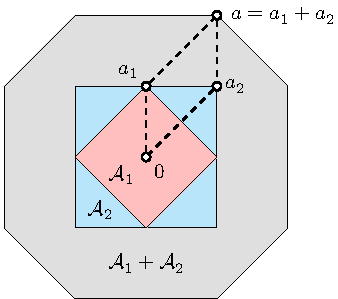
\includegraphics[page=1]{./figures/illustrations2.pdf}
    \caption{The sum of two atomic sets. The sum \(\Ascr_1+\Ascr_2\) is the unit level set for the polar convolution $\gauge\Aso\maxconv\gauge\Ast$, i.e., $\Ascr_1+\Ascr_2 = \{a \mid \gauge\Aso\maxconv\gauge\Ast(a) \leq 1\}$.\label{fig:sum-sets}}
\end{figure}

The subdifferential properties of polar convolution facilitate our analysis and allow us to build an efficient algorithm that is practical for a range of problems. In particular, the polar convolution decouples under a duality correspondence built around the polarity of convex sets. Under such duality correspondence,
\[
  \gauge_{\scriptscriptstyle(\Ascr_1+\Ascr_2)\polar}
  = \gauge_{\scriptscriptstyle\Ascr_1\polar} + \gauge_{\scriptscriptstyle\Ascr_2\polar},
\]
which implies that the subdifferential decouples as 
$\partial \gauge_{\scriptscriptstyle(\Ascr_1+\Ascr_2)\polar} = \partial\gauge_{\scriptscriptstyle\Ascr_1\polar}+\partial\gauge_{\scriptscriptstyle\Ascr_2\polar}$. Thus, a subgradient computation, which is central to all first-order methods for convex optimization, can be implemented using only subdifferential oracles for each of the polar functions $\gauge_{\scriptscriptstyle\Ascr_i\polar}$. 

\subsection{Decompression and deconvolution} \label{sec:3-1-2}

The principle innovation of our approach to the demixing problem \eqref{eq:demixing-problem} is to decouple the recovery procedure into two stages: an initial \emph{decompression} stage meant to recover the superposition $\xagg$ from the vector of observations $b$, followed by a \emph{deconvolution} stage that separates the recovered superposition $\xagg$ into its constituent components $\{x\nai\}_{i=1}^k$. We couple the convex theory of polar convolution~\citep{friedlander2019polarconvolution} to the theory of statistical dimension and signal incoherence to derive a recovery procedure and analysis for demixing a compressively sampled mixture to within a prescribed accuracy.

\paragraph{Stage 1: Decompression} The initial decompression stage is based on the observation
that because each signal $x\nai$ is $\Ascr_i$ sparse, the superposition $\xagg$
must be sparse with respect to the weighted vector sum
\begin{equation} \label{eq:weighted-atomic-sum}
  \Ascr\subs\coloneqq\sum_{i=1}^k\lambda_i\Ascr_i
  ~\equiv \left\{\sum_{i=1}^k\lambda_ia_i ~\bigg\vert~ a_i\in\Ascr_i\cup\{0\},\ i\in\irange1k\right\}
\end{equation}
of the individual atomic sets $\Ascr_i$. The positive weights $\lambda_i$ carry information about the relative powers of the individual signals, and serve to equilibrate the gauge values of each signal. Thus, the weights $\lambda_i$ are defined so that for each $i\in\irange1k$,
\begin{equation}\label{eq-lambda-def}
  \gauge_{\scriptscriptstyle\lambda_i\Ascr_i}(x\nai)=\gauge\Aso(x\nao). 
\end{equation}
The initial decompression stage solves the convex optimization problem
\begin{equation} \tag{P1} \label{eq:decompression}
  \minimize{x\in\Re^n}\enspace \gauge\Ass(x) \enspace\st\enspace \|Mx - b\|_2 \leq \alpha,
\end{equation}
where the parameter $\alpha\ge0$ bounds the acceptable level of misfit between the linear model \(Mx\) and the observations $b$, and correspondingly reflects the anticipated magnitude of the noise $\eta$. It follows from~\eqref{eq-polar-convolution-sum} that the objective of \eqref{eq:decompression} is in fact the polar convolution of the individual weighted gauges:
\begin{equation*}
   \gauge_{\scriptscriptstyle\Ascr\subs}(x)
   = \gauge_{\scriptscriptstyle\lambda_1\Ascr_1}\maxconv\gauge_{\scriptscriptstyle\lambda_2\Ascr_2}\maxconv\cdots\ \maxconv\gauge_{\scriptscriptstyle\lambda_k\Ascr_k}(x).
\end{equation*}
\autoref{thm-stability} establishes conditions under which the solution $x\subs^*$ to~\eqref{eq:decompression} stably approximates the superposition $\xagg$.

\paragraph{Stage 2: Deconvolution} The solution $x\subs^*$ of the decompression problem \eqref{eq:decompression} defines the subsequent convex deconvolution problem
\begin{equation} \tag{P2} \label{eq:deconvolution}
  \minimize{x_1, \ldots, x_k}
  \enspace \max_{i\in1:k}\, \gauge_{\scriptscriptstyle\lambda_i\Ascr_i}(x_i)
  \enspace\st\enspace
  \textstyle\sum_{i = 1}^k x_i = x\subs^*
\end{equation}
to obtain approximations $x_i^*$ to each constituent signal $x\nai$. 

In both stages, a variant of the conditional-gradient method provides a
computationally and memory efficient algorithm that can be implemented with
storage proportional to the number of measurements $m$~\citep{fan2019alignment}. We
describe in \autoref{ch:App-AtomicOpt} the details of the method.

\subsection{Related work}

\begin{table}[t]
  \begin{center}
  \begin{tabular}{lc@{\enspace}c@{\enspace}c@{\enspace}c@{\enspace}c} 
  \toprule
            & Compressed   & Noisy        & Number& Recovery  & Explicit \\
  Reference & measurements & observations & of signals  & algorithm & error bound\\\midrule
  \citep{mccoy2014convexity} & \xmark & \xmark & $2$  &\cmark  &\xmark\\
  \citep{mccoy2014sharp} & \xmark & \xmark & $2$ & \xmark & \cmark \\
  \citep{oymak2017universality} & \cmark & \xmark & $2$ &\xmark & \cmark \\
  \citep{mccoy2013achievable} & \cmark & \cmark & $\geq 2$ &\xmark & \xmark \\
  This paper & \cmark & \cmark & $\geq 2$ & \cmark & \cmark \\\bottomrule 
  \end{tabular}
  \end{center}
  \caption{Comparison of the main mathematical results obtained by this paper and related references. Only this paper and~\citet{mccoy2013achievable} consider the case of two or more signals.} \label{tab:comparasion}
\end{table}

The history of signal demixing can be traced to early work in seismic imaging~\citep{claerbout1973robust} and morphological component analysis~\citep{starck2005morphological,bobin2007morphological}, which used 1-norm regularization to separate incoherent signals. More recently,~\citet{mccoy2014sharp,mccoy2013achievable} and \citet{oymak2017universality} proposed a unified theoretical framework for signal demixing using modern tools from high-dimensional geometry.

\citet{mccoy2014convexity} analyzed the recovery guarantees of a convex program that can reconstruct $k = 2$ randomly-rotated signals from a full set of noiseless observations, i.e., $M$ is the identity matrix and $\norm{\eta}=0$. They also provided an ADMM-type algorithm for solving their proposed model. \citet{mccoy2014sharp} enhanced the error bound analysis under the same problem setting. \citet{mccoy2013achievable} subsequently extended this framework to demixing $k \geq 2$ randomly-rotated signals from noisy measurements, as modeled by~\eqref{eq:demixing-problem}. However, the constants in the recovery error bound are not made explicit. We postpone to \autoref{sec:comparasion} a detailed comparison between our theoretical results and theirs. \citet{oymak2017universality} considered a demixing problem similar to~\eqref{eq:deconvolution} that also incorporates the measurement operator $M$, and provided guarantees for demixing two unknown vectors from random and noiseless measurements. We build on this line of work by providing explicit recovery error bounds in terms of the complexity of the signal sets and the number of measurements. Our analysis allows for any number of individual signals $k\ge2$. Moreover, we provide a memory-efficient algorithm for solving our proposed model. \autoref{tab:comparasion} compares main mathematical results obtained by this paper and the above references.

Early work on demixing sparse signals implicitly assumed some notion of incoherence between representations of the signals. This concept was made concrete by \citet{doh01}, and subsequently \citet{doe03}, who measured the mutual incoherence of finite bases via the maximal inner-products between elements of the sets. Related incoherence definitions appear in compressed sensing~\citep{tro04, maleki2009coherence} and robust PCA~\citep{candes2011robust, wright2013compressive}. In this paper we adopt \citet{mccoy2013achievable}'s notion of incoherence as the minimal angle between conic representation of the individual signals.

\subsection{Roadmap}

\autoref{sec:3-2} shows that the decompression problem \eqref{eq:decompression} can stably recover $x\nag$. \autoref{thm:tropp} characterizes the recovery error in terms of the overall complexity of the signal, provided the measurements are random. This result follows directly from \citet{tropp2015convex} and a conic decomposition property particular to polar convolution. \autoref{sec:3-3} shows that the deconvolution problem~\eqref{eq:deconvolution} can stably approximate each $x\nai$. The bound in the recovery error is given in terms of the error in the initial decompression process and the incoherence between signals as measured by the minimum angle between conic representations of each signal; see \autoref{thm-stability}. This result requires a general notion of incoherence based on the angle between descent cones, first analyzed by \citet{mccoy2013achievable}.  \autoref{sec-incoherence} shows how a random-rotation model yields a particular level of incoherence with high probability; see \autoref{thm:Incoherence}. We develop the recovery guarantee under the random-rotation model; see \autoref{corollary-stability}. \autoref{sec:3-5} describes experiments on real and synthetic structured signals. Proofs of all theoretical results are given in \autoref{sec:3-7}.

The following blanket assumption holds throughout this chapter.
\begin{assumption}[Measurement model]\label{assume-blanket}
  The linear model~\eqref{eq:demixing-problem} satisfies the following conditions: the linear map
  $M:\Re^n\to\Re^m$ has i.i.d.\@ standard Gaussian entries; the noise vector $\eta$ satisfies $\|\eta\|_2\leq \alpha$ for some scalar $\alpha$; and the relative signal powers $\{\lambda_i\}_{i=1}^k$ satisfy~\eqref{eq-lambda-def}.
\end{assumption} 


\section{Decompressing the superposition}\label{sec:3-2} 

\begin{figure}[t]
    \centering
   \includegraphics[page=7]{./figures/illustrations2} 
  \caption{A non-trivial intersection of $\Dscr(\Ascr, x\na)$ and $\Null(M)$ is required for successful decompression. The blue shaded region represents the shifted descent cone $x\na + \Dscr(\Ascr, x\na)$, and red line represents the shifted null space $\Null(M) + x\na$. If $\Dscr(\Ascr, x\na) \cap \Null(M) \neq \{0\}$ (as depicted here) then there exists a vector $\hat x$ such that  $\gauge\As(\hat x) < \gauge\As(x\na)$ and $M\hat x = Mx\na$.\label{fig:descent-cone}}
\end{figure}

As shown in \autoref{sec:3-1-2}, under the assumption that the individual signals $x\nai$ are $\Ascr_i$ sparse, the aggregate signal $\xagg$ is sparse with respect to the aggregate atomic set $\Ascr\subs$.
Thus, the decompression of the observations $b$ in \eqref{eq:demixing-problem} is accomplished by minimizing the gauge to $\Ascr\subs$ to within the bound on the noise level $\|\eta\|_2\le\alpha$, as modeled by the recovery problem \eqref{eq:decompression}.
Without noise (i.e, $\alpha=0$), the aggregate signal $\xagg$ is the unique solution to \eqref{eq:decompression} when the null space of the measurement operator $M$ has only a trivial intersection with the descent cone $\Dscr\subs\coloneqq\Dscr(\Ascr\subs, \xagg)$.
In other words, $\xagg$ is the unique solution of \eqref{eq:decompression} if and only if 
\begin{equation}\label{eq-unique-optimality}
  \Dscr\subs\cap\Null(M) = \{0\}.  
\end{equation}
\autoref{fig:descent-cone} illustrates the geometry of this optimality condition, and depicts a case in which it doesn't hold.

If the linear operator $M$ is derived from Gaussian measurements, \citet{gordon1988milman} characterized the probability of the event~\eqref{eq-unique-optimality} as a function of the Gaussian width of the descent cone $\Dscr\subs$ and the number of measurements $m$. This result is the basis for recovery guarantees developed by \citet{chandrasekaran2012convex} and \citet{tropp2015convex} for a convex formulation similar to \eqref{eq:decompression}.

Intuitively, the number of measurements required for stable recovery of the aggregate $\xagg$ depends on the total complexity of the $k$ constituent $\Ascr_i$-sparse vectors $x\nai$. The complexity is measured in terms of the statistical dimension of each of the descent cones $\Dscr_i$.
\citet{tropp2015convex} established a bound on the recovery error between the solutions of the decompression problem~\eqref{eq:decompression} and the superposition $x\nag$ that depends on the statistical dimension $\delta(\Dscr\subs)$ of its descent cone. The following proposition is a restatement of \citep[Corollary~3.5]{tropp2015convex} applied to the decompression problem \eqref{eq:decompression}.

\begin{proposition}[Stable decompression of the aggregate]%
    \label{thm:tropp}
    For any $t>0$, any solution $x^*$ of \eqref{eq:decompression} satisfies
    \begin{equation*}
        \|x^* - \xagg\|_2 \leq 2\alpha\left[\sqrt{m - 1} - \sqrt{\delta(\Dscr\subs)} - t\right]_+^{-1}
    \end{equation*}
    with probability at least $1 - \exp(-t^2/2)$, where $[\xi]_+=\max\{0,\xi\}$. 
\end{proposition}

The statistical dimension of $\Dscr\subs$ is in general challenging to compute. However, we show in \autoref{sec:3-3-1} that when all the signals $\{x\nai\}_{i=1}^k$ are incoherent, a reasonable upper bound on $\delta(\Dscr\subs)$ can be guaranteed; see \autoref{coro:bound_sta_dim}.

As we can see from~\autoref{thm:tropp}, the recovery error bound has a linear dependence with the noise level $\alpha$. This result relies on the assumption that the noise level is over-estimated, i.e. $\alpha \geq \|\eta\|_2$; see~\autoref{assume-blanket}. However, when the noise level is under-estimated, i.e., $\alpha < \|\eta\|_2$, we can not provide any meaningful recovery error bound. This discussion suggests that if in practice, we don't know the true noise level, then we can start with a relative large $\alpha$, and keep reducing it until we get some reasonably good results.

\section{Deconvolving the components}\label{sec:3-3}

The second stage of our approach is the deconvolution stage which separates the recovered aggregate signal into its constituent components. In order to successfully separate the aggregate $x\nag$ into its components $\{x\nai\}_{i=1}^k$ using the deconvolution problem \eqref{eq:deconvolution}, additional assumption on dissimilarity between the atomic representations of the individual signals is generally required. For example, it can be challenging to separate the superposition of two sparse signals or two low-rank signals without additional assumptions. We follow \citet{mccoy2013achievable}, and measure the dissimilarity between signal structures---and thus their incoherence---using the angles between corresponding descent cones.

\begin{figure}[t]
    \centering
    \begin{tabular}{@{}cccc@{}}
      \includegraphics[width=.22\textwidth, page=3]{./figures/illustrations2}
    & \includegraphics[width=.22\textwidth, page=4]{./figures/illustrations2}
    & \includegraphics[width=.22\textwidth, page=5]{./figures/illustrations2}
    & \includegraphics[width=.22\textwidth, page=6]{./figures/illustrations2}
  \\ (a) \small $\Dscr_1\coloneqq\Dscr(\Ascr_1, x_1\na)$ & (b) \small  $\Dscr_2\coloneqq\Dscr(\Ascr_2, x_2\na)$ & (c) \small $d \in -\Dscr_1\cap\Dscr_2$ & (d) \small $x_1\na - d$ and $x_2\na + d$ 
    \end{tabular}
    \caption{The top row depicts two scaled atomic sets $\gauge\Aso(x_i\na)\cdot\Ascr_i$ and the corresponding descent cones $x_i\na + \Dscr_i$ (shifted to lie at $x_i\na$) for $i=1,2$. (c) The descent cones shifted to $x\na = x_1\na + x_2\na$, with $\Dscr_1$ negated; the vector $d$ lies in their intersection. (d) The vector $d$ descends on both scaled atomic sets, so that $\gauge\Aso(x_1\na - d) < \gauge\Aso(x_1)$ and $\gauge\Ast(x_2\na + d) < \gauge\Ast(x_2\na)$.}
    \label{fig:angle_cone}
\end{figure}

To motivate the incoherence definition, consider the case where there are only $k=2$ signals $x\nao$ and $x\nat$. If the descent cones $-\Dscr_1$ and $\Dscr_2$ have a nontrivial intersection, then there exists a nonzero direction $d \in -\Dscr_1 \cap \Dscr_2$ such that $\gauge\Aso(x\nao - d)<\gauge\Aso(x\nao)$ and $\gauge\Ast(x\nat + d)<\gauge\Ast(x\nat)$, which contradicts the optimality condition required for $x\nao$ and $x\nat$ to be unique minimizers of \eqref{eq:deconvolution}.  Thus, deconvolution only succeeds if the descent cones have a trivial intersection, which can be characterized using angle between the descent cones. \autoref{fig:angle_cone} illustrates this geometry. 

\citet{obert1991angle} defined the angle between two cones $\Kscr_1$ and $\Kscr_2$ in $\Re^n$ as the minimal angle between vectors in these two cones. It follows that the cosine of the angle between two cones can be expressed as 
\begin{equation*}
\cos\angle(\Kscr_1, \Kscr_2) 
= \sup\left\{\ip{x}{y} \mid x \in \Kscr_1\cap\mS^{n - 1},\, y \in \Kscr_2\cap\mS^{n - 1}\right\}.
\end{equation*}
For the general case where the number of signals $k\ge2$, a natural choice for a measure of incoherence between these structured signals is the minimum angle between the descent cone of a signal with respect to the remaining descent cones. 

\begin{definition} \label{def:incoherence}
    The pairs $\{(x\nai, \Ascr_i)\}_{i=1}^k$ are $\beta$-incoherent with $\beta\in(0,1]$ if for all $i\in\irange1k$,
    \[
        \cos\angle\left({-\Dscr_i},\, \sum_{j \neq i}\Dscr_j\right)
        \leq 1 - \beta. 
    \]
\end{definition}

We use the incoherence between descent cones to bound the error between the true constituent signals $\{x\nai\}_{i=1}^k$ and the solution set of the deconvolution problem~\eqref{eq:deconvolution}. This bound depends on the accuracy of the approximation $x\subs^*$ to the true superposition $x\nag$ and is shown in \autoref{thm-stability}.

\begin{proposition}[Stable deconvolution]\label{thm-stability} 
    If the pairs $\{(x\nai, \Ascr_i)\}_{i=1}^k$ are $\beta$-incoherent for some $\beta\in(0,1]$, then any set of solutions $\{x_i^*\}_{i=1}^k$ of~\eqref{eq:deconvolution} satisfies for all $i\in\irange1k$
    \begin{align*}
        \|x_i^* - x\nai\|_2 \leq \|x\subs^*-\xagg\|_2/\sqrt{\beta},
    \end{align*}
    where $x\subs^*$ is any solution of~\eqref{eq:decompression}.
\end{proposition}

In summary, a large angle between negation of a descent cone $-\Dscr_i$ and all the other descent cones---as reflected by a large incoherence constant $\beta$---corresponds a small error between each $x_i^*$ and the ground truth $x\nai$.

\subsection{Bound on \texorpdfstring{$\delta(\Dscr\subs)$}{Ds} under incoherence}\label{sec:3-3-1}

\autoref{thm:tropp} gives a stable recovery result for the decompression stage. However, the recovery bound depends on the the statistical dimension of $\Dscr\subs$, which is challenging to compute even when the statistical dimension of the individual descent cone $\Dscr_i$ is known. In this section, we show that the incoherence between the structured signals $\{x\nai\}_{i=1}^k$ is sufficient to establish an upper bound for $\delta(\Dscr\subs)$. 
We start with the $k = 2$ case. \autoref{prop:bound_sta_dim} shows that if the angle between two cones is bounded, then the statistical dimension of the sum of these two cones is also bounded. 

\begin{proposition}[Bound on statistical dimension of sum]\label{prop:bound_sta_dim}
    Let $\Kscr_1$ and $\Kscr_2$ be two closed convex cones in $\Re^n$. If $\cos\angle(-\Kscr_1, \Kscr_2) \leq 1 - \beta$ for some $\beta \in (0, 1]$, then 
    \[\sqrt{\delta(\Kscr_1 + \Kscr_2)} \leq \tfrac{1}{\sqrt{\beta}}\left(\sqrt{\delta(\Kscr_1)} + \sqrt{\delta(\Kscr_2)} \right).\]
\end{proposition}

This result generalizes to an arbitrary number of cones. 
\begin{corollary}[Bound on statistical dimension of sum under incoherence]\label{coro:bound_sta_dim}
   If the pairs $\{(x\nai, \Ascr_i)\}_{i=1}^k$ are $\beta$-incoherent for some $\beta\in(0,1]$, then
   \[\sqrt{\delta(\Dscr\subs)} \leq \beta^{-\tfrac{k-1}{2}}\sum_{i=1}^k\sqrt{\delta(\Dscr_i)}.\]
\end{corollary} 
\autoref{coro:bound_sta_dim} shows that when the pairs $\{(x\nai, \Ascr_i)\}_{i=1}^k$ are $\beta$-incoherent, $\delta(\Dscr\subs)$ can be upper bounded in terms of the statistical dimension of individual descent cones.

\section{Inducing incoherence through random rotation}\label{sec-incoherence}

\autoref{thm-stability} establishes the stability of the deconvolution problem in the case that the unknown signals are $\beta$-incoherent, as formalized in \autoref{def:incoherence}. However, except in very special cases like randomly rotated signals, it is not feasible to determine the incoherence constant $\beta$. We build on McCoy and Tropp's random rotation model~\citep{mccoy2013achievable} to quantify, with high probability, the $\beta$-incoherence of $k$ randomly-rotated atomic sparse signals, and present a recovery result for a randomly rotated case.

We first consider a simpler case of two general cones, one of which is randomly rotated. Let $\SO(n)$ denote the special orthogonal group, which consists of all $n$-by-$n$ orthogonal matrices with unit determinant. The following proposition provides a probabilistic bound on the angle between the two cones in terms of their statistical dimension. This geometric result maybe of intrinsic interest in other contexts.

\begin{proposition}[Probabilistic bound under random rotation] \label{prop-angle-cones}
    Let $Q$ is drawn uniformly at random from $\SO(n)$. Let $\Kscr_1$ and $\Kscr_2$ be two closed convex cones in $\Re^n$. For any $t \geq 0$, we have
\[\mP\bigg[\cos\angle(\Kscr_1, Q\Kscr_2) \geq  \tfrac{3}{\sqrt{n}}\left(\sqrt{\delta(\Kscr_1)} + \sqrt{\delta(\Kscr_2)}\right) + t\bigg] \leq \exp(-\tfrac{n-2}{8}t^2). \]
\end{proposition}

We now assume that the $k$ structured signals $x\nai$ are defined via a random rotations of $k$ underlying structured signals $x_i^\circ$.
\begin{assumption}[Random rotations]\label{assume-random-rotation}
   Fix $x_i^\circ$ and $\Ascr_i^\circ$ for $i\in\irange1k$ such that $x_i^\circ$ is sparse with respect to atomic set $\Ascr_i^\circ$. For each $i\in\irange1k$, assume 
  \begin{equation*}
    x\nai \coloneqq Q_i  x_i^\circ \quad\mbox{and}\quad \Ascr_i \coloneqq  Q_i \Ascr_i^\circ,
  \end{equation*}
  where the matrices $Q_i$ are drawn uniformly and i.i.d.\@ from $\SO(n)$.
\end{assumption}

Our next proposition shows that, under mild conditions, randomly rotated structured signals are incoherent with high probability. 
\begin{proposition} \label{thm:Incoherence}
    Suppose that \autoref{assume-random-rotation} holds. If 
    \[\sum_{i=1}^k \sqrt{\delta(\Dscr_i)} \leq \left(1 - 4^{- \tfrac{1}{k-1} } - t\right)\sqrt{n} / 6\] 
    for some $t>0$, then the rotated pairs $\{(x\nai,\Ascr_i)\}_{i=1}^k$ are $4^{- \tfrac{1}{k-1} }$-incoherent with probability at least $1 - k(k-1)\exp(-\tfrac{n-2}{8}t^2)$.
\end{proposition}

\autoref{thm:Incoherence} requires $\sum_{i=1}^k \sqrt{\delta(\Dscr_i)}$ to scale as $\sqrt{n}$ and thus controls the total complexity of the $k$ unknown signals. We now state the main theorem and show that randomly rotated vectors can be recovered using the two-stage approach~\eqref{eq:decompression} and~\eqref{eq:deconvolution}.

\begin{theorem} \label{corollary-stability}
    Suppose that \autoref{assume-blanket} and \autoref{assume-random-rotation} hold. For any $t_1, t_2 > 0$, if $\sum_{i=1}^k \sqrt{\delta(\Dscr_i)} \leq \left(1 - 4^{- \tfrac{1}{k-1} } - t_2\right)\sqrt{n} / 6$, then any set of minimizers $\{x_i^*\}_{i=1}^k$ of~\eqref{eq:deconvolution} satisfies 
  \begin{equation} \label{eq:theory_bound}
    \|x_i^* - x\nai\|_2 
     \leq
     4\alpha\,\left[\sqrt{m-1} - c\sum_{i=1}^k \sqrt{\delta(\Dscr_i)} - t_1\right]_+^{-1}
  \end{equation}
   for all $i\in\irange1k$ with probability at least $1 - \exp\left(-t_1^2/2\right) - k(k-1)\exp(-\tfrac{n-2}{8}t_2^2)$ and $c\leq2$.
\end{theorem}
The proof follows directly from \autoref{thm:tropp}, \autoref{thm-stability}, \autoref{coro:bound_sta_dim}, \autoref{thm:Incoherence}, and the probability union bound. We verify empirically in \autoref{sec:3-5-1} the tightness of the bound in~\eqref{eq:theory_bound}.

\subsection{Comparison of error bound} \label{sec:comparasion}

Here we compare our results to the one provided in \citep{mccoy2013achievable}, which also developed a novel procedure to solve the demixing problem \eqref{eq:demixing-problem}. In \citep{mccoy2013achievable}, the authors introduced the constrained optimization problem
\begin{equation}
    \label{eq:achievable-model}
    \begin{array}{ll}
    \minimize{x_1,\ldots,x_k}
    & \left\|
      M^\dagger\left(M\sum_{i=1}^k x_i - b\right)
    \right\|_2 \\
   \st
    & \gauge\Asi(x_i) \le \gauge\Asi(x\nai), \ \forall i\in\irange1k,
    \end{array}
\end{equation}
where $M^\dagger$ is the Moore-Penrose pseudo-inverse of $M$ and showed that if \(n\ge m\ge \sum_{i=1}^k\delta(\Dscr_i)+\BigOh(\sqrt{kn})\) and $\{x\nai\}_{i=1}^k$ are randomly rotated as per \autoref{assume-random-rotation}, then any set of minimizers $\{x_i^*\}_{i=1}^k$ of~\eqref{eq:achievable-model} satisfies with high probability the bound
\begin{equation}\label{eq:Tropp_error}
    \|x_i^*-x\nai\|_2\le C\|M^\dagger\eta\|_2
\end{equation}
for all $i\in\irange1k$~\cite[Theorem~A]{mccoy2013achievable}. To our knowledge, this result is the first to show that stable recovery of the constituent signals $\{x\nai\}_{i=1}^k$ is possible with high probability provided the number of measurement grow linearly in $k$. However, the constant $C$ in the error bound \eqref{eq:Tropp_error} could depend on all of the problem parameters except $\eta$. As a comparison to \autoref{corollary-stability}, the error bound in \eqref{eq:theory_bound} makes explicit the effect of all problem parameters.

\section{Experiments and novel applications} \label{sec:3-5}

In~\autoref{sec:3-5-1} we empirically verify \autoref{corollary-stability} through a set of synthetic experiments on recovering multiple randomly-rotated sparse signals from noiseless and noisy measurements. Note that the random rotation guarantees incoherence among the unknown signals $\{x\nai\}_{i=1}^k$. We also empirically show that random rotation is not required for successful recovery of a class of unknown signals with different underlying structures. In~\autoref{sec:3-5-2} we separate a sparse signal and sparse-in-frequency signal. In~\autoref{sec:3-5-3} we separate the superposition of three signals: a sparse signal, a low-rank matrix, and noise. In~\autoref{sec:3-5-4} we separate a multiscale low-rank synthetic image.

The optimization problems are solved using the Julia package \texttt{AtomicOpt.jl} that will be introduced in \autoref{ch:App-AtomicOpt}. All the experiments are conducted on a Linux server with 8 CPUs and 64Gb memory.

\subsection{Stability of Demixing} \label{sec:3-5-1}

We provide three experiments that numerically verify the bounds established by \autoref{corollary-stability} to solve the demixing problem \eqref{eq:demixing-problem}. The experiment draws multiple realizations of a random problem specified over a range of parameters $k$ (number of signals), $m$ (number of measurements), $n$ (signal dimension) and $s$ (the sparsity level for each signal). Each signal $x\nai$ in~\eqref{eq:demixing-problem} is generated according to \autoref{assume-random-rotation}, where each vector $x_i^\circ$ is $s$-sparse with respect to the standard basis. By construction, the atomic sets $i\in\irange1k$ are defined to be 
\[
  \Ascr_i = Q_i \{\pm e_1, \dots, \pm e_n\}\text{where} Q_i\sim\uniform(\SO(n)).
\]
\citet[Proposition~4.5]{amelunxen2014living} give an upper bound on the statistical dimension of the descent cone for $(x\nai,\Ascr_i)$, and thus for the descent cone at $(x_i^\circ,\Ascr_i^\circ)$, for  $s$-sparse vectors. We use this bound to approximate the statistical dimension $\delta(\Dscr_i)$ of the descent cone $\Dscr_i$ corresponding to the pair $(x\nai,\Ascr_i)$.  We define the maximum absolute error
\begin{equation} \label{eq:rela_diff}
  \mathop{\tt maxerr}\coloneqq \max_{i\in\irange1k}\ \twonorm{x_i^*-x\nai}.
\end{equation}

\subsubsection{Relation between $m$ and $n$} \label{sec:phase_transition1}
We first show a phase portrait for the noiseless case that verifies the relationship between number of measurement $m$ and signal dimension $n$, as stated in \autoref{corollary-stability}. The number of signals is fixed at $k=3$ and the sparsity level is fixed at $s=5$. The phase plot is shown in \autoref{fig:phase_transition1}, where the horizontal axis represents the signal dimension $n\in\{50, 65, \dots, 500\}$ and the vertical axis represents the number of measurements $m\in\{50, 65, \dots, 500\}$. The colormap indicates the empirical probability of successful demixing over 50 trials, where we say the demixing is successful if $\mathop{\tt maxerr} < 10^{-2}$. The red solid curve and the blue dashed line, respectively, approximate the graphs of the functions
\[\sqrt{m} = \sum_{i=1}^k \sqrt{\delta(\Dscr_i)}\text{and}\sqrt{n} = \sum_{i=1}^k \sqrt{\delta(\Dscr_i)}.\]
The statistical dimensions of $\Dscr_i$ are approximated using ~\citep[Proposition~4.5]{amelunxen2014living}, as stated above. The area above the red curve and to the right of the dashed line corresponds to problem parameters with successful recovery and corroborates the bounds stated in \autoref{corollary-stability}.

\begin{figure}[t]
    \centering
    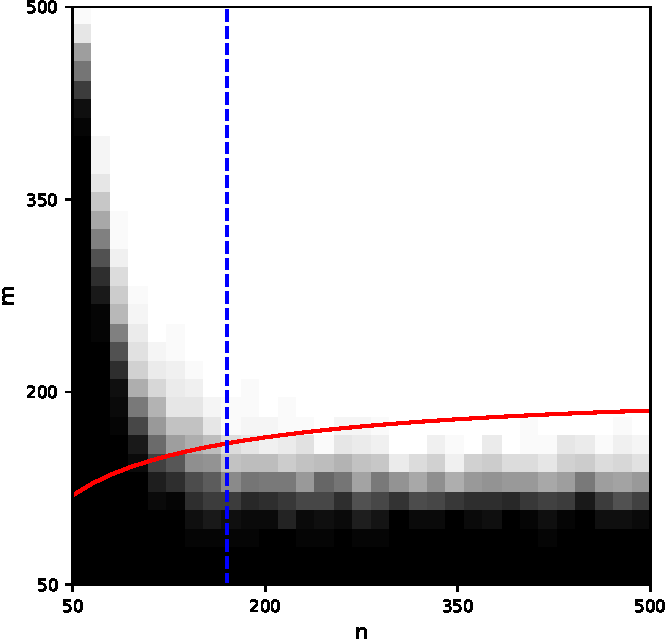
\includegraphics[width=.5\linewidth]{./figures/relation_m_n.pdf}
    \caption{Phase-transition plots for demixing the sum of randomly-rotated sparse signals $\{x\nai\}_{i=1}^k$ from noiseless measurements $b$. The horizontal and vertical axes, respectively, represent the signal dimension $n$ and measurement dimension $m$. The colormap indicates the empirical probability of successful demixing over 50 trials. The red solid curve approximately represents the mapping $\sqrt{m} = \sum_{i=1}^k \sqrt{\delta(\Dscr_i)}$ and the blue dashed line approximately represents the position $\sqrt{n} = \sum_{i=1}^k \sqrt{\delta(\Dscr_i)}$.}
    \label{fig:phase_transition1}
\end{figure}

\subsubsection{Relation between $m$ and $k$}
We also show a phase portrait for the noiseless case that verifies the relationship between number of measurement $m$ and number of signals $k$ stated in \autoref{corollary-stability}. The signal dimension is fixed at $n=1000$ and the sparsity level is fixed at $s=3$. The phase plot is shown in \autoref{fig:phase_transition2}, where the horizontal axis represents the number of signals $k\in\{2, 3, \dots, 10\}$ and the vertical axis represents the number of measurements $m\in\{100, 200, \dots, 1000\}$. All the other settings are the same as stated in \autoref{sec:phase_transition1}. The red line corresponds to $\sqrt{m} = \sum_{i=1}^k \sqrt{\delta(\Dscr_i)}$ and shows that recovery is possible provided the number of measurements scale as $k^2$, when the complexity of all of unknown signals are the same.

\begin{figure}[t]
    \centering\small
    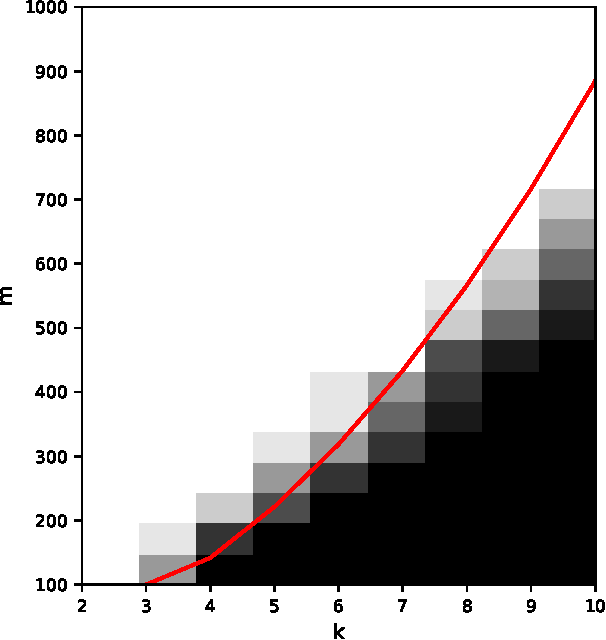
\includegraphics[width=.5\linewidth]{./figures/relation_m_k.pdf}
    \caption{Phase-transition plots for demixing the sum of randomly-rotated sparse signals $\{x\nai\}_{i=1}^k$ from noiseless measurements $b$. The horizontal and vertical axes, respectively, represent the number of signals $k$ and measurement dimension $m$. The colormap indicates the empirical probability of successful demixing over 50 trials. The red solid curve approximately represents the mapping $\sqrt{m} = \sum_{i=1}^k \sqrt{\delta(\Dscr_i)}$.}
    \label{fig:phase_transition2}
\end{figure}

\subsubsection{Relation between maximal absolute error and noise level}
Lastly, we show a plot for the noisy case that verifies the relationship between maximum absolute error $\mathop{\tt maxerr}$ and noise level $\alpha$ stated in \autoref{corollary-stability}. The number of measurement is fixed at $m=125$, the signal dimension is fixed at $n=200$, the number of signals is fixed at $k=3$, and the sparsity level is fixed at $s=5$. The result is shown in \autoref{fig:phase_transition3}, where the horizontal axis represents the noise level $\alpha\in\{0.01, 0.02, \dots, 2\}$ and the vertical axis represents the maximum absolute error $\mathop{\tt maxerr}$. The blue curve corresponds to the mean of $\mathop{\tt maxerr}$ over 50 trials and the yellow shaded area corresponds to the standard deviation. The figure verifies the linear dependence of the recovery error with the noise level, as stated in \autoref{corollary-stability}.

\begin{figure}[t]
    \centering\small
    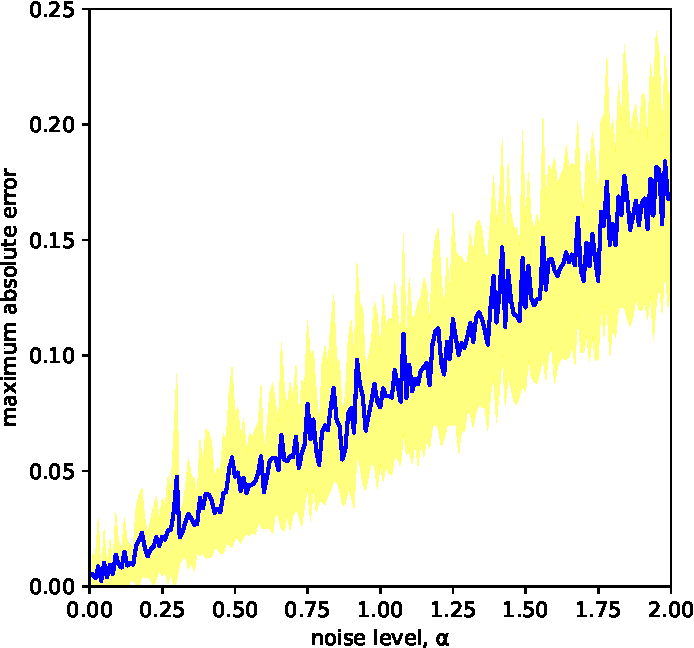
\includegraphics[width=.5\linewidth]{./figures/relation_e_noise.pdf}
    \caption{Error-noise plot for demixing the sum of randomly-rotated sparse signals $\{x\nai\}_{i=1}^k$ from noisy measurements $b$. The horizontal and vertical axes, respectively, represent the noise level $\alpha$ and the maximum absolute error $\mathop{\tt maxerr}$. The blue curve indicates the relationship between the empirical average of $\mathop{\tt maxerr}$ over 50 trials and $\alpha$, and the yellow shaded area indicated the empirical standard deviation. }
    \label{fig:phase_transition3}
\end{figure}


\subsection{Separation of sparse and sparse-in-frequency signals} \label{sec:3-5-2}

\begin{figure}[t]
    \centering
   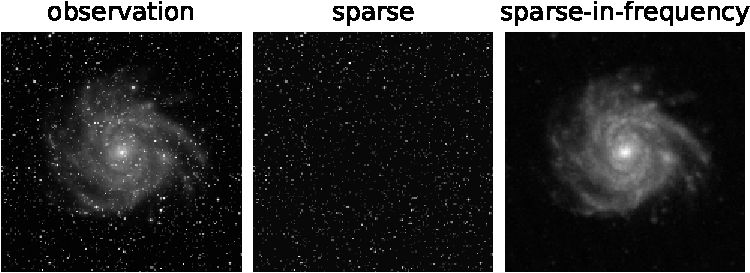
\includegraphics[width=.9\textwidth]{./figures/StarGalaxy.pdf}
    \caption{The star-galaxy separation experiment features two distinct signal components. The image size is $601\times601$ pixels.}
    \label{fig:star_galaxy}
\end{figure}

We reproduce the experiments done by \citet{mccoy2014convexity} on separating an astronomical image into a sparse and a sparse-in-frequency signals. An $n$-vector $x$ is sparse-in-frequency if its discrete cosine transform (DCT) $Dx$ is sparse, where the orthogonal linear map $D:\Re^n\to\Re^n$ encodes the DCT. Define the observations and corresponding atomic sets
\[
  b = x\na_s + x\na_d,
  \quad
  \Ascr_s \coloneqq  \{\pm e_1, \dots, \pm e_n\}, \quad \Ascr_d = D^*\Ascr_s.
\]
The star-galaxy image shown in \autoref{fig:star_galaxy} exemplifies this superposition: the stars are well-represented by sparse matrices in $\Ascr_s$, and the galaxy component is well-represented by sinusoidal elements in $\Ascr_d$. The image size is $601\times601$. The results of the separation are shown in the second two panels of \autoref{fig:star_galaxy}.

\subsection{Sparse and low rank matrix decomposition with structured noise}\label{sec:3-5-3}

In this next example we decompose an image that contains a sparse foreground, a low-rank background, and structured noise. This is an example of sparse principle component analysis~\citep{fazel1998approximations,fhb01,pati1994phase,valiant1977graph}. Typically, the entry-wise 1-norm and the nuclear norm are used to extract from the matrix each of these qualitatively different structures. Here, we treat the noise as its own signal that also needs to be separated. We consider the observations
\[B = X\na_s + X\na_l + X\na_n,\]
where $X\na_s\in\Re^{m\times n}$ is sparse, $X\na_l\in\Re^{m\times n}$ is low-rank matrix, and $X\na_n\in\Re^{m\times n}$ represents structured noise so that $PX\na_nQ$ is sparse, where $P$ and $Q$ are random orthogonal $m$-by-$m$ matrices. Based on the atomic framework, we choose the atomic sets for $X\na_s$, $X\na_l$, and $X\na_n$, respective, as
\begin{align*}
    \Ascr_s &= \{\pm E_{i,j} \mid 1 \leq i \leq m, 1 \leq j \leq n \},
  \\\Ascr_l &= \{uv^\intercal \mid u \in \Re^m,\ v \in \Re^n,\ \|u\|_2=\|v\|_2 = 1\},
  \\\Ascr_n &= P^\intercal\Ascr_s Q^\intercal,
\end{align*}
where $E_{i,j}$ is a $m\times n$ matrix with a single nonzero entry $(i,j)$ with value $1$. 

For the numerical experiment, we consider the noisy chess board in-painting problem. The chess foreground is sparse and the chess board background is low rank. The image size is $596\times596$. The experiment result is shown in~\autoref{fig:chess_board}. 

\begin{figure}[t]
    \centering
    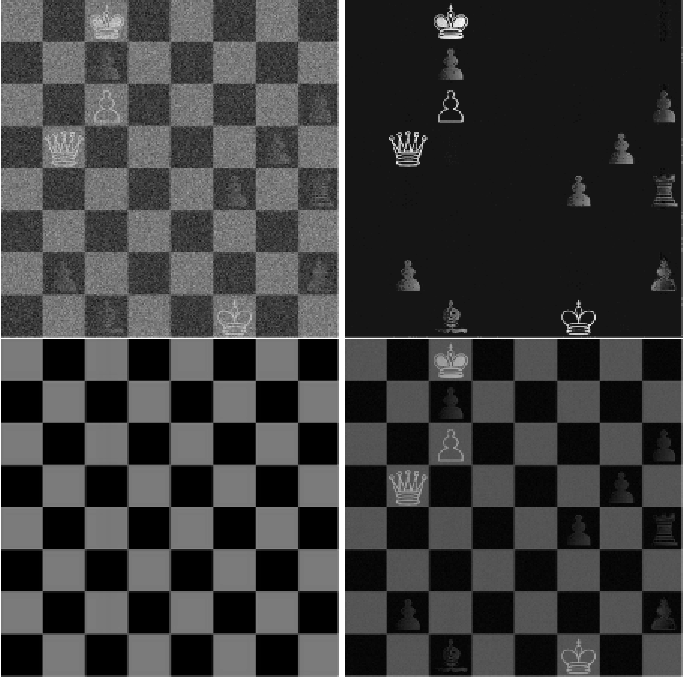
\includegraphics[width=.6\textwidth]{./figures/ChessBoard.pdf}
    \caption{Noisy chess board in-painting experiment. The image size is $596\times596$. Northwest: noisy observations; Northeast: recovered sparse component; Southwest: recovered low rank component; Southeast: denoising result.}
    \label{fig:chess_board}
\end{figure}

\subsection{Multiscale low rank matrix decomposition} \label{sec:3-5-4}

The multiscale low-rank matrix decomposition problem proposed by \citet{ong2016beyond} generalizes the sparse and low-rank matrix decomposition through a block-wise low-rank structure. Let $X$ be an $m \times n$ matrix and $\Pscr$ be a partition of $X$ into multiple blocks. Then $X$ is considered to be block-wise low-rank with respect to $\Pscr$ if all the blocks are low rank. For each block $p\in\Pscr$ with size $m_p \times n_p$, let $X_p$ denote the corresponding part of the matrix $X$ and let $R_p: \Re^{m \times n} \to \Re^{m_p \times n_p}$ denote the linear operator that can extract $X_p$ from $X$, namely $R_p(X) = X_p$. The adjoint operator $R_p^*: \Re^{m_p \times n_p} \to \Re^{m \times n}$ embeds an $m_p \times n_p$ matrix into a $m \times n$ zero matrix. With this operator, 
\begin{equation*}
  X = \sum\limits_{p \in \Pscr} R_p^*(X_p).
\end{equation*}

Each block-wise low-rank signal is represented by a corresponding atomic set. By definition, each block $X_p \in \Re^{m_p \times n_p}$ is low rank, and thus $X_p$ is $\Ascr_p$-sparse, where 
\[
  \Ascr_p = \left\{uv^\intercal \mid u \in \Re^{m_p}, v \in \Re^{n_p}, \|u\| = \|v\| = 1\right\}.
\]
One and Lustig~\cite{ong2016beyond} propose a block-wise nuclear norm and its associated dual norm, respectively, by the functions 
\[
  \|\cdot\|_{\Pscr,1} = \textstyle \sum_{p \in \Pscr} \|R_p(\cdot)\|_1,
  \quad
  \|\cdot\|_{\Pscr,\infty} = \max_{p \in \Pscr} \|R_p(\cdot)\|_{\infty},
\]
where $\|\cdot\|_1$ and $\|\cdot\|_\infty$ are the Schatten 1- and $\infty$-norms of their matrix arguments. It follows that the block-wise norm $\|\cdot\|_{\Pscr,1}$ and dual norm $\|\cdot\|_{\Pscr,\infty}$ are the gauge and support functions, respectively, for the atomic set $\Ascr_\Pscr \coloneqq  \bigcup_{p \in \Pscr} R_p^*\Ascr_p$.

We reproduce the synthetic model described by Ong and Lustig, who construct the superposition $B = \sum_{i = 1}^k X\nai$,
where $X\nai \in \Re^{m \times n}$ is block-wise low rank with respect to the multiscale partitions $\{\Pscr_i\}_{i = 1}^k$. In our experiment, we set $m = n = 64$, $k = 4$, and for each $i\in\irange1k$,
\[m_p = n_p = 4^{i-1}  \quad \forall p \in \Pscr_i.\]
At the lowest scale $i=1$, a block-wise low-rank matrix is a scalar, and so 1-sparse matrices are included with the atomic set $\Ascr_{\Pscr_1}$.  The solutions of the deconvolution procedure \autoref{eq:deconvolution} are shown in~\autoref{fig:multiscale}.

\begin{figure}[t]
    \centering
    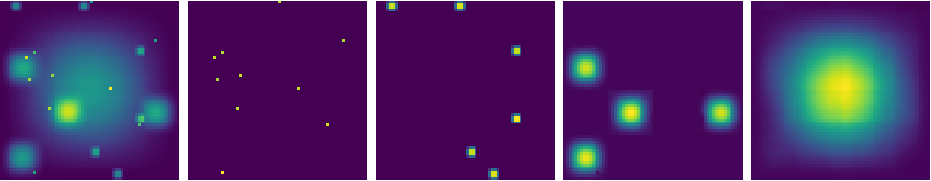
\includegraphics[width=\textwidth]{./figures/Multiscale.pdf}
    \caption{Multiscale low rank matrix decomposition experiment. The matrix size is $64\times64$. From left to right: observations; recovered $\Pscr_i$-block-wise low rank component for $i = 1,\dots,4$. All the blocks in $\Pscr_i$ have the same size $4^{i-1}\times4^{i-1}$ for $i = 1,\dots,4$.}
    \label{fig:multiscale}
\end{figure}

\section{Summary of contributions}\label{sec:3-6}

In this chapter, we study the structural signal demixing problem. We develop a two-stage, decompression-deconvolution approach for compressed signal demixing motivated by the polar convolution of gauge functions and the polar alignment property developed in \autoref{ch:Dual-Struc-Opt}. Under the assumption of Gaussian measurements and randomly rotated signals, we develop explicit signal-recovery error and sample complexity bounds for the two-stage approach. These are the first known explicit error bounds for recovering an arbitrary number of mixed and compressed signals. Extensive numerical experiments on synthetic and real data verify the correctness of our theoretical results and the effectiveness of our approach.




\section{Proofs} \label{sec:3-7}

This section contains proofs for the mathematical statements in this chapter. We begin with several technical results needed for analysis, which describe useful properties of descent cones. Some of these results contain their own intrinsic interest.

\subsection{Lemmas} \label{sec:3-7-1}

\begin{lemma}[Properties of descent cones]\label{prop-descent-cone-properties} Let $\Ascr$, $\Ascr_1$, $\Ascr_2$ be compact sets in $\Re^n$ that contain the origin in their interiors. Fix the vectors $x, x_1, x_2$. The following properties hold.
    \begin{itemize}
     \item[(a)] \label{prop-descent-cone-properties-a}
       A vector $d$ is contained in $\Dscr(\Ascr, x)$ if and only if there is some $\bar\alpha > 0$ such that $\gauge\As(x + \alpha d) \leq \gauge\As(x)$ for all $\alpha \in [0, \bar\alpha]$;
     \item[(b)] \label{prop-descent-cone-properties-b}
       $\Dscr(\tau\Ascr, x) = \Dscr(\Ascr, x)\ \forall\tau > 0$;
     \item[(c)] \label{prop-descent-cone-properties-c}
       $\Dscr(Q\Ascr, Qx) = Q\Dscr(\Ascr, x)$ if $Q\in \SO(n)$;
     \item[(d)] \label{prop-descent-cone-properties-d}
       $\Dscr(\Ascr_1 + \Ascr_2, x_1 + x_2) \subseteq \Dscr(\Ascr_1, x_1) + \Dscr(\Ascr_2, x_2)$ if $\gauge\Aso(x_1) = \gauge\Ast(x_2)$.
     \end{itemize}
\end{lemma} 

\begin{proof}
    \leavevmode
      \begin{itemize}
        \item[(a)] See \citep[Proposition 2.5]{mccoy2014sharp};
        \item[(b)] It follows from the fact that a gauge function is positive homogenous.  
        % \[\Dscr(\tau\Ascr, x) = \cone\set{d \mid \gauge_{\tau\Ascr}(x + d) \leq \gauge_{\tau\Ascr}(x)} = \cone\set{d \mid \gauge_{\Ascr}(x + d) \leq \gauge_{\Ascr}(x)}.\]
        \item[(c)] Because $\gauge_{Q\Ascr}=\gauge_\Ascr(Q^*\cdot)$,
        \begin{align*}
          \Dscr(Q\Ascr, Qx) &= \cone\{d \mid \gauge_{Q\Ascr}(Qx + d) \leq \gauge_{Q\Ascr}(Qx)\}
          \\&= \cone\{d \mid \gauge_{\Ascr}(x + Q^*d) \leq \gauge_{\Ascr}(x)\}
          \\&= Q\Dscr(\Ascr, x).
        \end{align*}
        \item[(d)] 
        For every $d \in \Dscr(\Ascr_1 + \Ascr_2, x_1 + x_2)$, by \autoref{prop-descent-cone-properties-a}(a), there exists $\alpha > 0$ such that  
        \[\gauge\Asum(x_1 + x_2 + \alpha d) \leq \gauge\Asum(x_1 + x_2).\] 
        Then there exists $d_1, d_2$ such that $d_1 + d_2 = \alpha d$ and 
        \[\max\{\gauge\Aso(x_1 + d_1), \gauge\Ast(x_2 + d_2)\} \leq \gauge\Asum(x_1 + x_2).\]
        By the fact that $\gauge\Asum(x_1 + x_2) \leq \max\{\gauge\Aso(x_1), \gauge\Ast(x_2)\}$ and the assumption $\gauge\Aso(x_1) = \gauge\Ast(x_2)$, it follows that $d_i \in \Dscr(\Ascr_i, x_i)$, which implies $\alpha d = d_1 + d_2 \in \Dscr(\Ascr_1, x_1) + \Dscr(\Ascr_2, x_2)$. Thus $d \in \Dscr(\Ascr_1, x_1) + \Dscr(\Ascr_2, x_2)$.
      \end{itemize}
\end{proof}

The Gaussian width of a set $T \subset \Re^n$ is defined as
\[\omega(T) = \mE_{g} \sup\{ \ip{g}{y} | y\in T\},\]
where the expectation is taken with respect to the standard Gaussian $\Nscr(0,I_n)$. 
The following lemma summarizes the main properties that we use regarding the relationship between the conic summaries $\delta$ and $\omega$.

\begin{lemma}[Properties of conic statistical summaries]\label{prop:stat_dim}
    Let $\Kscr$ be a closed and convex cones in $\Re^n$ and let $Q\in\SO(n)$. Then the following properties hold. 
    \begin{itemize}
      \item[(a)] \label{prop:stat_dim_a} $\delta(Q\Kscr) = \delta(\Kscr)$;
      \item[(b)] \label{prop:stat_dim_b} $\delta(\Kscr) = \mE_g \left[\sup\{ \ip{g}{y} | y\in\Kscr\cap\mB^n\}^2\right]$;
      \item[(c)] \label{prop:stat_dim_c} $\omega(\Kscr\cap\mB^n)^2 \leq \delta(\Kscr)$.
    \end{itemize}
\end{lemma}

\begin{proof} 
    See \citep[Proposition~3.1(6) and Proposition~3.1(5)]{amelunxen2014living}, respectively, for (a) and (b). 
    \begin{itemize}
      \item[(c)] Indeed, we know that,
      \begin{align*}
        \omega(\Kscr\cap\mB^n)^2 &= \left[\mE_{g} \sup\{ \ip{g}{y} | y\in \Kscr\cap\mB^n\}\right]^2
        \\&\leq \mE_{g} \left[\sup\{ \ip{g}{y} | y\in \Kscr\cap\mB^n\}^2\right]
        \\&= \delta(\Kscr),
      \end{align*}
      where the first equality follows from the definition of gaussian with, the first inequality follows from the fact that $\mE(X)^2 \leq \mE(X)^2$ for any random variable $X$, and the last equality follows from \autoref{prop:stat_dim_b}(b). 
    \end{itemize}
\end{proof}

Our next lemma shows that if the angle between two cones is bounded, then the norms of individual vectors are bounded by the norm of their sum.

\begin{lemma}\label{lemma:bound_norm}
    Let $\Kscr_1$ and $\Kscr_2$ be two closed convex cones in $\Re^n$. If $\cos\angle(-\Kscr_1, \Kscr_2) \leq 1 - \beta$ for some $\beta \in (0, 1]$, then for any $u \in \Kscr_1$ and $v \in \Kscr_2$, 
    \[\max\{\|u\|, \|v\|\} \leq \frac{1}{\sqrt{\beta}}\|u + v\|.\]
\end{lemma}

\begin{proof}
    By expanding the norm square of $u + v$ we can get that 
      \begin{align*}
        \|u + v\|^2 &= \|u\|^2 + \|v\|^2 - 2\ip{-u}{v}
        \\&= \|u\|^2 + \|v\|^2 - 2\cos(\angle(-u, v))\|u\|\|v\|
        \\&\geq \|u\|^2 + \|v\|^2 - 2(1-\beta)\|u\|\|v\|
        \\&= \beta(\|u\|^2 + \|v\|^2) + (1-\beta)(\|u\| - \|v\|)^2
        \\&\geq \beta\max\{\|u\|^2, \|v\|^2\},
      \end{align*}
    where the first inequality follows from the definition of the cosine of the angle between two cones. 
\end{proof}

Our next lemma is a technical lemma for the expectation.

\begin{lemma}\label{lemma:expectation}
    Let $X$ and $Y$ be nonnegative random variables, then we have 
    \[\mE[(X+Y)^2] \leq \left( \sqrt{\mE[X^2]} + \sqrt{\mE[Y^2]} \right)^2.\]
\end{lemma}

\begin{proof}
    By expanding the right hand side, we can get
    \begin{align*}
      \left( \sqrt{\mE[X^2]} + \sqrt{\mE[Y^2]} \right)^2 &= \mE[X^2] + \mE[Y^2] + 2\sqrt{\mE[X^2]\mE[Y^2]}
      \\&\geq \mE[X^2] + \mE[Y^2] + 2\mE[XY]
      \\&= \mE[(X+Y)^2],
    \end{align*}
    where the inequality follows from the Cauchy–Schwarz inequality.
\end{proof}

\subsection{Proof for \titlelink{\autoref{thm-stability}}} \label{sec:proof-thm-stability}
For each $i\in\irange1k$, let $\epsilon_i \coloneqq  x_i^* - x\nai$ and $\epsilon_{-i} : = \sum_{j \neq i}\epsilon_j$. By the definition of descent cone,
$\epsilon_i \in \Dscr(\Ascr_i, x\nai$).
Because $\{(x\nai, \Ascr_i)\}_{i=1}^k$ are $\beta$-incoherent for some $\beta\in(0,1]$, by~\autoref{def:incoherence},
\[\cos\angle\left(-\epsilon_i, \epsilon_{-i}\right) \leq 1 - \beta.\]
By \autoref{lemma:bound_norm}, it follows that
\[ \left\|\epsilon_i + \epsilon_{-i}\right\| \geq \sqrt{\beta}\|\epsilon_i\|.\]
The desired result follows.

\subsection{Proof for \titlelink{\autoref{prop:bound_sta_dim}}} \label{sec:proof-bound_sta_dim}
In this proof, we define $\Kscr_{i, \beta} =  \Kscr_i \cap \tfrac{1}{\sqrt{\beta}} \mB^n$ and $f_{i, \beta}(g) = \sup\{ \ip{g}{u} | u \in \Kscr_{i, \beta}\}$ for $i = 1, 2$. By \autoref{prop:stat_dim_b}, we know that the statistical dimension can be expressed as
\begin{align*}
  \delta(\Kscr_1 + \Kscr_2) &= \mE_g \left[\sup\{ \ip{g}{y} | y\in(\Kscr_1 + \Kscr_2)\cap\mB^n\}^2 \right]
  \\&= \mE_g \left[\sup\{ \ip{g}{u + v} | u \in \Kscr_1, v \in \Kscr_2, \|u + v\| \leq 1 \}^2\right]
  \\&\leq \mE_g \left[\sup\{ \ip{g}{u + v} | u \in \Kscr_{1, \beta}, v \in \Kscr_{2, \beta} \}^2\right]
  \\&= \mE_g \left[ \left(\sup\{ \ip{g}{u} | u \in \Kscr_{1, \beta}\} + \sup\{ \ip{g}{v} | v \in \Kscr_{2, \beta}\} \right)^2 \right]
  \\&\leq \left( \sqrt{ \mE_g \left[ f_{1, \beta}(g)^2 \right]} + \sqrt{ \mE_g \left[ f_{2, \beta}(g)^2 \right]} \right)^2
  % \\&= \left( \tfrac{1}{\sqrt{\beta}} \sqrt{ \mE_g \left[ \sup\set{ \ip{g}{u} | u \in \Kscr_1 \cap \mB^n}^2 \right]} + \tfrac{1}{\sqrt{\beta}} \sqrt{ \mE_g \left[ \sup\set{ \ip{g}{v} | v \in \Kscr_2 \mB^n}^2 \right]} \right)^2
  \\&= \tfrac{1}{\beta}\left(\sqrt{\delta(\Kscr_1)} + \sqrt{\delta(\Kscr_2)} \right)^2
\end{align*}
where the first inequality follows from \autoref{lemma:bound_norm} and the fact that the supremum is always nonnegative, and the second inequality follows from \autoref{lemma:expectation}. 

\subsection{Proof for \titlelink{\autoref{coro:bound_sta_dim}}} \label{sec:proof-coro-bound_sta_dim}
Throught this proof, for all $i\in1:k$, we define $\Dscr_i = \Dscr(\Ascr_i, x\nai)$, $\delta_i = \delta(\Dscr_i)$ and $\delta_{1:i} = \delta(\sum_{j=1}^i\Dscr_i)$. By \autoref{assume-blanket} and \autoref{prop-descent-cone-properties-d}, we know that $\Dscr\subs \subseteq \sum_{i=1}^k \Dscr_i$, and it follows that $\delta(\Dscr\subs)\leq\delta_{1:k}$. So we only need to give an upper bound for $\delta_{1:k}$. Since $\cos\angle\left({-\Dscr_k},\, \sum_{i=1}^{k-1}\Dscr_i\right)\leq 1 - \beta$, by \autoref{prop:bound_sta_dim}, it follows that 
\begin{equation} \label{eq:111}
  \sqrt{\delta_{1:k}} \leq \beta^{-\tfrac{1}{2}}\left(\sqrt{\delta_{1:(k-1)}} + \sqrt{\delta_k}\right).
\end{equation}
Since $\sum_{i=1}^{k-2}\Dscr_i \subseteq \sum_{j\neq(k-1)}\Dscr_j$, it follows that $\cos\angle\left({-\Dscr_{k-1}},\, \sum_{i=1}^{k-2}\Dscr_i\right)\leq  1 - \beta$. By \autoref{prop:bound_sta_dim}, we have 
\begin{equation} \label{eq:112}
  \sqrt{\delta_{1:(k-1)}} \leq \beta^{-\tfrac{1}{2}}\left(\sqrt{\delta_{1:(k-2)}} + \sqrt{\delta_{k-1}}\right).
\end{equation}
Combining \eqref{eq:111} and \eqref{eq:112}, we know that 
\[\sqrt{\delta_{1:k}} \leq \beta^{-\tfrac{2}{2}}\left(\sqrt{\delta_{1:(k-2)}} + \sqrt{\delta_{k-1}} + \sqrt{\delta_k}\right).\]
Repeating this process, we can conclude that 
\[\sqrt{\delta_{1:k}} \leq \beta^{-\tfrac{k-1}{2}}\sum_{i=1}^k\sqrt{\delta_i}.\]

\subsection{Proof for \titlelink{\autoref{prop-angle-cones}}}\label{sec:proof-prop-angle-cones}
Throught this proof, we define the following notations:
\begin{itemize} 
  \item $\overline\Kscr_i:=\Kscr_i\cap\mS^{n-1}$ for $i=1,2$;
  \item $\widehat\Kscr_i:=\Kscr_i\cap\mB^n$ for $i=1,2$;
  \item $f(W\in\Re^{n\times n}) = \sup\{\ip{x}{Wy} \mid x \in \overline\Kscr_1, y \in\overline\Kscr_2\}$;
  \item $\hat f(W\in\Re^{n\times n}) = \sup\{\ip{x}{Wy} \mid x \in \widehat\Kscr_1, y \in\widehat\Kscr_2\}$;
  \item $\Oscr_n = \{Q\in\Re^{n\times n}: Q^TQ = I_n\}$;
  \item $\Sscr\Oscr_{n, +} = \{Q\in\Oscr_n: \det(Q) = 1\}$;
  \item $\Sscr\Oscr_{n, -} = \{Q\in\Oscr_n: \det(Q) = -1\}$.
\end{itemize} 

Our proof consists of three steps. 

\paragraph{First step: show that both $f$ and $\hat f$ are convex and $1$-Lipschitz functions.} First, we show that both $f$ and $\hat f$ are convex. 
For any $W_1, W_2 \in \Re^{n\times n}$ and any $t \in [0,1]$, 
\begin{align*}
  &f(tW_1 + (1-t)W_2) 
  \\&= \sup\{\ip{x}{(tW_1 + (1-t)W_2)y} \mid x \in \overline\Kscr_1, y \in\overline\Kscr_2\}
  \\&= \sup\{\ip{x}{tW_1y} + \ip{x}{(1-t)W_2y} \mid x \in \overline\Kscr_1, y \in\overline\Kscr_2\}
  \\&\leq tf(W_1) + (1-t)f(W_2).
\end{align*}
So $f$ is convex. The same reason holds for $\hat f$, and thus $\hat f$ is also convex. 
Next, by \citep[Lemma~2.6]{shalev2011online}, in order to show that both $f$ and $\hat f$ are $1$-Lipschitz, we only need to show that the norm of any subgradient of $f$ or $\hat f$ is bounded by $1$. By \citep[Theorem~D.4.4.2]{hiriart-urruty01}, we know that for any $W \in \Re^{n\times n}$, 
\begin{align*}
  \partial f(W) &= \conv\{xy^T \mid x \in \overline\Kscr_1, y \in\overline\Kscr_2, \ip{x}{Wy} = f(W)\},
  \\ \partial \hat f(W) &= \conv\{xy^T \mid x \in \widehat\Kscr_1, y \in\widehat\Kscr_2, \ip{x}{Wy} = f(W)\}.
\end{align*}
Since $\|x\| \leq 1$ and $\|y\| \leq 1$, it is easy to verify that for any $W\in\Re^{n\times n}$ and for any $Z \in \partial f(W) \cup \partial \hat f(W)$, 
\[\|Z\|_F \leq 1,\]
where $\|\cdot\|_F$ is the Frobenius norm. Therefore, we can conclude that both $f$ and $\hat f$ are $1$-Lipschitz functions.


\paragraph{Second step: bound $\mE_{Q \sim \uniform(\Sscr\Oscr_{n, +})}\left[f(Q)\right]$.} 
First, we give the bound on 
\[\mE_{Q \sim \uniform(\Oscr_n)}\left[\hat f(Q)\right].\] 
From the first step, we know that $\hat f$ is convex. Then by the comparison principle developed by Tropp; see \citep[Theorem~5 and Lemma~8]{tropp2012comparison}, we can conclude that 
\begin{equation} \label{eq:help1}
  \mE_{Q \sim \uniform(\Oscr_n)}\left[\hat f(Q)\right] \leq \tfrac{1.5}{\sqrt{n}}\mE_{G\sim\Nscr(0, I_n)}\left[\hat f(G)\right],
\end{equation}
Next, we give the bound on $\mE_{Q \sim \uniform(\Sscr\Oscr_{n, +})}\left[\hat f(Q)\right]$. By expanding the uniform distribution over $\Oscr_n$, we can get
\begin{align*}
  &\mE_{Q \sim \uniform(\Oscr_n)}\left[\hat f(Q)\right] 
  \\&= \tfrac{1}{2}\mE_{Q \sim \uniform(\Sscr\Oscr_{n, +})}\left[\hat f(Q)\right] + \tfrac{1}{2}\mE_{Q \sim \uniform(\Sscr\Oscr_{n, -})}\left[\hat f(Q)\right]
  \\&\geq \tfrac{1}{2}\mE_{Q \sim \uniform(\Sscr\Oscr_{n, +})}\left[\hat f(Q)\right],
\end{align*}
where the inequality follows from the fact that $\hat f$ is non-negative. Combine this result with \eqref{eq:help1}, we can conclude that 
\begin{equation} \label{eq:help2}
  \mE_{Q \sim \uniform(\Sscr\Oscr_{n, +})}\left[\hat f(Q)\right] \leq \tfrac{3}{\sqrt{n}}\mE_{G\sim\Nscr(0, I_n)}\left[\hat f(G)\right].
\end{equation}
Then, by the Gaussian Chevet’s inequality; see\citep[Exercise~8.7.4]{vershynin2018high}, we know that 
\begin{equation} \label{eq:help3}
  \mE_{G\sim\Nscr(0, I_n)}\left[\hat f(G)\right] \leq \omega(\widehat\Kscr_1) + \omega(\widehat\Kscr_2) \leq \sqrt{\delta(\Kscr_1)} + \sqrt{\delta(\Kscr_2)},
\end{equation}
where the second inequality follows from \autoref{prop:stat_dim_c}. Combine \eqref{eq:help2} and \eqref{eq:help3}, we can get
\begin{equation} \label{eq:help4}
  \mE_{Q \sim \uniform(\Sscr\Oscr_{n, +})}\left[\hat f(Q)\right] \leq \tfrac{3}{\sqrt{n}}\left( \sqrt{\delta(\Kscr_1)} + \sqrt{\delta(\Kscr_2)} \right).
\end{equation}
Finally, by the fact that $f \leq \hat f$ and \eqref{eq:help4}, we can conclude that 
\begin{equation} \label{eq:help5}
  \mE_{Q \sim \uniform(\Sscr\Oscr_{n, +})}\left[f(Q)\right] \leq \tfrac{3}{\sqrt{n}}\left( \sqrt{\delta(\Kscr_1)} + \sqrt{\delta(\Kscr_2)} \right).
\end{equation}

\paragraph{Third step: concentration bound for $f(Q)$.}
From step 1, we know that $f$ is $1$-Lipschitz. For clearness, we denote $\mP_{Q \sim \uniform(\Sscr\Oscr_{n, +})}$ and $\mE_{Q \sim \uniform(\Sscr\Oscr_{n, +})}$ as $\mP_Q$ and $\mE_Q$. By the concentration bounds of Lipschitz functions over the special orthogonal group develop by Meckes; see \citep[Theorem~5.5 and Theorem~5.16]{meckes2019random}, we can get that for every $t\geq0$,
\[\mP_Q\left[f(Q) \geq \mE_Q[f(Q)] + t\right] \leq \exp(-\tfrac{n-2}{8}t^2).\]
Note that a similar result can be obtained from \citep[Theorem~5.2.7]{vershynin2018high}.
Combining with \eqref{eq:help5}, we can conclude that for every $t\geq0$,
\[\mP_Q\left[f(Q) \geq  \tfrac{3}{\sqrt{n}}\left( \sqrt{\delta(\Kscr_1)} + \sqrt{\delta(\Kscr_2)} \right) + t\right] \leq \exp(-\tfrac{n-2}{8}t^2).\]

\subsection{Lemmas needed for the proof of \titlelink{\autoref{thm:Incoherence}}} \label{sec:prob_bounds}
In this section, we present two lemmas that are needed for the proof of \autoref{thm:Incoherence}. These two lemmas provide probabilistic bound on the statistical dimension of sum of randomly rotated cones. 

The next lemma provides a probabilistic bound on the statistical dimension of the sum of two cones. 
\begin{lemma}[Probabilistic bound on statistical dimension under random rotation] \label{prop-bound-sta-dim}
   Let $\Kscr_1$ and $\Kscr_2$ be two closed convex cones in $\Re^n$. Then 
 \begin{align*}
   \mP\bigg[\sqrt{\delta(\Kscr_1 + Q\Kscr_2)} &\leq \tfrac{1}{\sqrt{\beta(t)}}\left(\sqrt{\delta(\Kscr_1)} + \sqrt{\delta(\Kscr_2)} \right) \bigg]
   \\&\geq 1 - \exp(-\tfrac{n-2}{8}t^2)
   \\\text{with} \beta(t) &= 1 - \tfrac{3}{\sqrt{n}}\left(\sqrt{\delta(\Kscr_1)} + \sqrt{\delta(\Kscr_2)}\right) - t ,
 \end{align*}
   where $Q$ is drawn uniformly at random from $\SO(n)$.
\end{lemma}

\begin{proof}
    By \autoref{prop:bound_sta_dim} and \autoref{prop-angle-cones}.
\end{proof}

Our next lemma extends \autoref{prop-bound-sta-dim} to arbitrary number of cones. 
\begin{lemma} \label{prop:bound-sum-sta-dim}
   Let $\Kscr_1, \dots, \Kscr_p$ be closed convex cones in $\Re^n$ and let $Q_1, \dots, Q_p$ be i.i.d. matrices uniformly drawn from $\SO(n)$. If $\sum_{i=1}^p \sqrt{\delta(\Kscr_i)} \leq \left(1 - 4^{- \tfrac{1}{p-1} } - t\right)\sqrt{n} / 6$ for some $t > 0$, then 
   \begin{equation*}
   \mP\left[ \sqrt{\delta\left(\sum_{i=1}^pQ_i\Kscr_i\right)} \leq 2\sum_{i=1}^p \sqrt{\delta(\Kscr_i)}\right] \geq 1 - (p-1)\exp(-\tfrac{n-2}{8}t^2).
   \end{equation*}
\end{lemma}

\begin{proof}
    Throughout this proof, we define the following notations:
    \begin{itemize}
      \item $\delta_i = \delta(\Kscr_i)$, for all $i\in1:p$;
      \item $\delta_{1:i} = \delta\left(\sum_{j=1}^iQ_j\Kscr_j\right)$, for all $i\in1:p$;
      \item For each $i\in2:p$, define the event 
    \begin{align*}
      E_i(t) &= \left\{ \sqrt{\delta_{1:i}} \leq \tfrac{1}{\sqrt{\beta_i(t)}} \left( \sqrt{\delta_{1:(i-1)}} + \sqrt{\delta_i}\right)\right\}
      \\\text{with} \beta_i(t) &= 1 - \tfrac{3}{\sqrt{n}}\left( \sqrt{\delta_{1:(i-1)}} + \sqrt{\delta_i}\right) - t.
    \end{align*}
    \end{itemize}
    
    Our proof consists of three steps.
    
    \paragraph{Step 1:} bound the probability of $E_2(t)\land\cdots\land E_p(t)$.
    Denote the indicator random variable for $E_i(t)$ by $\mathbbm{1}_{E_i(t)}$, which evaluates to $1$ if $E_i(t)$ occurs and otherwise evaluates to $0$. Then for each $i\in2:p$, we have
    \begin{align*}
      \mP(E_i(t)) &= \mE(\mathbbm{1}_{E_i(t)})
      \\&= \mE_{\{Q_j\}_{j=1}^{i-1}} \left[ \mE\left(\mathbbm{1}_{E_i(t)} \mid \{Q_j\}_{j=1}^{i-1}\right)\right]
      \\&\geq \mE_{\{Q_j\}_{j=1}^{i-1}} \left[ 1 - \exp(-\tfrac{n-2}{8}t^2) \right]
      \\&= 1 - \exp(-\tfrac{n-2}{8}t^2),
    \end{align*}
    where the inequality follows from \autoref{prop-bound-sta-dim} and the assumption that $Q_i$ are all independent. Extending the bound on $\mP(E_i(t))$ to all $i\in\irange2p$ via the union bound, we have
    \[
      \mP(E_2(t) \land\cdots\land E_p(t))
      \geq 1 - (p-1)\exp(-\tfrac{n-2}{8}t^2).\]
    
    \paragraph{Step 2:} show that $E_2(t) \land\cdots\land E_p(t)$ implies bound on \[\sqrt{\delta_{1:p}}\leq\tfrac{1}{\sqrt{\beta_2(t)\dots\beta_p(t)}}\sum_{i=1}^p\sqrt{\delta_i}.\] Indeed, we have 
    \begin{align*}
      \sqrt{\delta_{1:p}} &\leq \tfrac{1}{\sqrt{\beta_p(t)}}\left( \sqrt{\delta_{1:(p-1)}} + \sqrt{\delta_p}\right)
      \\&\leq \tfrac{1}{\sqrt{\beta_p(t)}}\left( \tfrac{1}{\sqrt{\beta_{p-1}(t)}}\left( \sqrt{\delta_{1:(p-2)}} + \sqrt{\delta_{p-1}}\right) + \sqrt{\delta_p}\right)
      \\&\leq \tfrac{1}{\sqrt{\beta_p(t)\beta_{p-1}(t)}}\left( \sqrt{\delta_{1:(p-2)}} + \sqrt{\delta_{p-1}} + \sqrt{\delta_p}\right)
      \\&\vdots
      \\&\leq \tfrac{1}{\sqrt{\beta_2(t)\dots\beta_i(t)}}\sum_{j=1}^i\sqrt{\delta_j}.
    \end{align*}
    
    \paragraph{Step 3:} show that $E_2(t) \land\cdots\land E_p(t)$ and the assumption \[\sum_{i=1}^p \sqrt{\delta(\Kscr_i)} \leq \left(1 - 4^{- \tfrac{1}{p-1} } - t\right)\sqrt{n} / 6\] implies that $\beta_i(t) \geq 4^{-\tfrac{1}{k-1} }$ for $i\in2:p$. We prove this by induction on $i$. First we show that $\beta_2(t) \geq 4^{-\tfrac{1}{k-1} }$. Indeed, we have 
    \begin{align*}
      \beta_2(t) &= 1 - \tfrac{3}{\sqrt{n}}\left( \sqrt{\delta_1} + \sqrt{\delta_2}\right) - t
      \\&\geq 1 - \tfrac{3}{\sqrt{n}}\tfrac{ \left(1 - 4^{- \tfrac{1}{k-1} } - t\right)\sqrt{n} }{6} - t
      \geq  4^{-\tfrac{1}{k-1} }.
    \end{align*}
     Next for any $i\in3:k$, we assume that $\beta_j(t) \geq 4^{-\tfrac{1}{k-1} }$ for all $2\leq j \leq (i-1)$, then we have 
    \begin{align*}
      \beta_i(t) &=  1 - \tfrac{3}{\sqrt{n}}\left( \sqrt{\delta_{1:(i-1)}} + \sqrt{\delta_i}\right) - t
      \\&\geq 1 - \tfrac{3}{\sqrt{n}} \tfrac{1}{\sqrt{\beta_2(t)\dots\beta_{i-1}(t)}}\sum_{j=1}^{i}\sqrt{\delta_j} - t
      \\&\geq 1 - \tfrac{3}{\sqrt{n}} 2^{ \tfrac{i-2}{k-1} } \tfrac{ \left(1 - 4^{- \tfrac{1}{k-1} } - t\right)\sqrt{n} }{6} - t
      \geq 4^{- \tfrac{1}{k-1} }.
    \end{align*}
    
    Finally, combining all three steps, we can conclude that 
    \begin{equation*}
      \mP\left[ \sqrt{\delta\left(\sum_{i=1}^pQ_i\Kscr_i\right)} \leq 2\sum_{i=1}^p \sqrt{\delta(\Kscr_i)}\right] \geq 1 - (p-1)\exp(-\tfrac{n-2}{8}t^2).
    \end{equation*}
\end{proof}

\subsection{Proof for \titlelink{\autoref{thm:Incoherence}}} \label{sec:proof-thm:Incoherence}

Throughout this proof, we define the following notations for all $i\in1:k$:
\begin{itemize} 
  \item $\Dscr_i = \Dscr(\Ascr_i, x\nai)$;
  \item $\hat \Dscr_i =  \Dscr(\hat \Ascr_i, \hat x\nai)$;
  \item $\delta_i = \delta(\Dscr_i)$;
  \item $\delta_{1:i} = \delta\left(\sum_{j=1}^i\Dscr_i\right)$;
  \item $\delta_{-i} = \delta\left(\sum_{j\neq i}\Dscr_j\right)$.
\end{itemize} 
By~\autoref{prop-descent-cone-properties-c}, for all $i\in1:k$, we have
\[\Dscr_i = \Dscr(Q_i \hat \Ascr_i, Q_i \hat x\nai) = Q_i\hat\Dscr_i.\]
Then it follows from \autoref{prop:stat_dim_a} that
\[\delta(\hat \Dscr_i) = \delta(Q_i^T \Dscr_i) = \delta_i.\]
For all $i\in\irange1k$, define 
\begin{itemize}
  \item $\hat \Dscr_i\coloneqq  \Dscr(\hat \Ascr_i, \hat x\nai)$;
  \item $\delta_i = \delta(\Dscr_i)$;
  \item $\delta_{-i} = \delta\left(\sum_{j\neq i}\Dscr_j\right)$
\end{itemize}
First, fix $t >0$, for each $i\in\irange1k$, define the event
\[
E_i(t) =  \left \{ \cos\angle\left(-\Dscr_i, \sum_{j \neq i}\Dscr_j\right) \leq \tfrac{3}{\sqrt{n}}\left(\sqrt{\delta_i} + \sqrt{\delta_{-i}}\right) + t \right\}.
\] 
Denote the indicator random variable for $E_i(t)$ by $\mathbbm{1}_{E_i(t)}$, which evaluates to $1$ if $E_i(t)$ occurs and otherwise evaluates to $0$. Then, the following chain of inequalities gives the upper bound for the probability of the event $E_i(t)$:
\begin{align} \label{eq:123}
  \begin{split}
\mP (E_i(t)) 
  &= \mE (\mathbbm{1}_{E_i(t)})
\\&= \mE_{\{Q_j\}_{j\ne i}} \mE\left[\mathbbm{1}_{E_i(t)} \bigm\vert Q_j\ \forall j\ne i \right]
\\&\geq \mE_{\{Q_j\}_{j\ne i}} [ 1 - \exp(-\tfrac{n-2}{8}t^2) ]
\\&= 1 - \exp(-\tfrac{n-2}{8}t^2),
\end{split}
\end{align}
where the inequality follows from \autoref{prop-angle-cones}. 

Next, by \autoref{prop:bound-sum-sta-dim}, we know that 
\begin{equation}\label{eq:223}
  \mP\left[ \sqrt{\delta_{-i}} \leq 2\sum_{j\neq i} \sqrt{\delta_j}\right] \geq 1 - (k-2)\exp(-\tfrac{n-2}{8}t^2).
\end{equation}


Thirdly, for each $i\in\irange1k$, define the event, 
\[
\hat E_i(t) =  \left \{ \cos\angle\left(-\Dscr_i, \sum_{j \neq i}\Dscr_j\right) \leq \tfrac{6}{\sqrt{n}}\sum_{i=1}^k\sqrt{\delta_i} + t\right \}.
\]
By combining \eqref{eq:123} and \eqref{eq:223} together, we can conclude that 
\[\mP(\hat E_i(t)) \geq 1 - (k-1)\exp(-\tfrac{n-2}{8}t^2).\]
Extend the bound on $\mP(\hat E_i(t))$ to all $i\in\irange1k$ via the union bound:
\[\mP(\hat E_1\land\cdots\land \hat E_k) \geq 1 - k(k-1)\exp(-\tfrac{n-2}{8}t^2).\]

Finally, by our assumption
\[\sum_{i=1}^k \sqrt{\delta(\Dscr_i)} \leq \left(1 - 4^{- \tfrac{1}{k-1} } - t\right)\sqrt{n} / 6,\] it follows that 
\[\tfrac{6}{\sqrt{n}}\sum_{i=1}^k\sqrt{\delta_i} + t \leq 1 - 4^{- \tfrac{1}{k-1} }.\]
Therefore, we can conclude that the rotated pairs $\{(x\nai,\Ascr_i)\}_{i=1}^k$ are $4^{- \tfrac{1}{k-1} }$-incoherent with probability at least $1 - k(k-1)\exp(-\tfrac{n-2}{8}t^2)$.












%    4. Primal-rerieval strategy for structured optimization
%% The following is a directive for TeXShop to indicate the main file
%%!TEX root = diss.tex
\chapter{Primal-retrieval strategy for structured optimization}
\label{ch:App-Primal-Retrieval}

\section{Introduction} \label{sec:4-1}

Consider the problem of fitting a model to data by selecting model parameters as the superposition of a limited set atomic elements taken from a given dictionary. Versions of this cardinality-constrained problem appear in a number of statistical-learning applications in machine learning \cite{tibshirani1996regression,yul06,Meinshausen06,aep08}, data mining, and signal processing~\cite{candes:2013}. In these applications, common atomic dictionaries include the set of one-hot vectors or matrices, rank-1 unit matrices, usually chosen as a mechanism to encode a notion of parsimony in the definition of the model parameters.

The formulation we consider takes the form
\begin{equation} \label{eq:main_prob} 
    \find x\in\Re^n \sut f(b - Mx) \leq \alpha \tand \card_\Ascr(x) \leq k,
\end{equation}
where $f:\Re^n\to\Re$ is an $L$-smooth and convex function, $M: \Re^n \to \Re^m$ is a linear operator with $m < n$, $b \in \Re^m$ is the observation vector, and $\Ascr \subseteq \Re^n$ is the atomic dictionary. The cardinality function 
\begin{equation}\label{eq-card-fcn}
    \card_\Ascr(x) \coloneqq \inf\left\{ \mathbf{nnz}(c) ~\bigg\vert~ x = \textstyle\sum\limits_{a \in \Ascr} c_a a, \enspace c_a \geq 0\right\}
\end{equation}
measures the complexity of $x$ with respect to the atomic set $\Ascr$.  The loss term $f(b - Mx)$ measures the quality of the fit. When $\Ascr = \{ \pm e_1,\pm e_2, \ldots,\pm e_n \}$ is the set of signed canonical unit vectors, the function $\card_\Ascr(x)$ simply counts the number of nonzero elements in $x$. Typically $k\ll n$, which indicates that we seek a feasible model parameter $x$ that has an efficient representation in terms of the atoms in $\Ascr$.

For the application areas that we hope to target, the two characteristics of this feasibility problem that pose the biggest challenge to efficient implementation are the combinatorial nature of the cardinality constraint, and the high-dimensionality of the parameter space. To address the combinatorial challenge, we follow van den Berg and Friedlander~\cite{berg2008probing,berg2011sparse} and Chandrasekaran et al.~\cite{chandrasekaran2012convex}, and use the convex gauge function as a tractable proxy for the cardinality function~\eqref{eq-card-fcn}; see \eqref{eq:gauge1}. In tandem with the convexity of the loss function, this function allows us to formulate three alternative relaxed convex optimization problems that under certain conditions have approximate solutions that satisfy the feasibility problem; see problems~\eqref{prob:primal1},~\eqref{prob:primal2}, and~\eqref{prob:primal3} in \autoref{sec:4-2}. 

The high-dimensionality of the parameter space, however, may imply that it's inefficient---and maybe even practically impossible---to solve these convex relaxations because it's infeasible to directly store the approximations to a feasible solution $x$. Instead, we wish to develop methods that leverage the efficient representation that feasible solutions have in terms of the atoms in the dictionary $\Ascr$. For example, consider the case in which the dictionary is the set of ${n \times n}$ rank-one matrices, and $M$ is the trace linear operator that maps these matrices into $m$-vectors. Any method that iterates directly on the parameters $x$ requires $\BigOh(n^2+m)$ storage. An alternative is the widely-used conditional gradient method \cite{frank1956algorithm}, which requires $\BigOh( n t+m )$ storage after $t$ iterations~\cite{jaggi2013revisiting}, but also often requires a substantial number of iterations $t$ to converge. Instead of storing $x$ directly, we use the dual problems to the convex relaxations ~\eqref{prob:primal1},~\eqref{prob:primal2}, and~\eqref{prob:primal3}, which require only $\BigOh(m)$ storage, and still allow us to collect information on which atoms in $\Ascr$ participate in the construction of a feasible $x$.

\subsection{Approach}

We propose a unified algorithm-agnostic strategy that uses any sequence of improving dual solutions to one of the convex relaxations to identify an essential subset of atoms in $\Ascr$ needed to construct an $\epsilon$-infeasible solution $x$ that satisfies
\begin{equation} \label{eq:feasible}
    f(b - Mx) \leq \alpha + \epsilon \tand \card(\Ascr; x) \leq k
\end{equation}
for any positive tolerance $\epsilon$. These \emph{atomic-identification} rules, described in \autoref{sec:atom_iden}, derive from the polar-alignment property and apply to arbitrary dictionaries $\Ascr$ \cite{fan2019alignment}. These atom-identification rules generalize earlier approaches described by El~Ghaoui~\cite{Ghaoui12} and Hare and Lewis~\cite{hare2004identifying}. Once an essential subset of $k$ atoms is identified, an $\epsilon$-feasible solution $x$ can be computed by optimizing over all positive linear combinations of this subset. This relatively small $k$-variable problem can often be solved efficiently.

We prove that when the atomic dictionary is polyhedral, we can set $\epsilon$ to zero and still identify in polynomial time a set of feasible atoms; see \autoref{coro:polyhedral}. When the atomic dictionary is spectrahedral, we prove that an $\epsilon$-feasible set of atoms can be identified also in polynomial time; see \autoref{coro:spectral}. 

We demonstrate via numerical experiments on real-world datasets that this approach is effective in practice.

There are three important components in our primal-retrieval algorithm. The first is an arbitrary iterative oracle $\texttt{oracle}_{f,\Ascr,M,b}(\cdot)$ that can generate iterates $y^{(t)}$ converging to the optimal dual variable $y^*$ of any of the dual problem \Drobi. The second is an atom-identifier $\texttt{EssCone}_{\Ascr, M, k}(\cdot)$ which can map a dual variable $y$ to the cone generated from the essential atoms identified by $y$ such that any element in this cone will have cardinality at most $k$, i.e., 
\begin{equation} \label{eq:ess_cone}
  \texttt{EssCone}_{\Ascr, M, k}(y) \subseteq \{x \mid \card(A; x) \leq k\}.
\end{equation}
We make the definition of the function $\texttt{EssCone}_{\Ascr, M, k}$ explicit when the atomic set $\Ascr$ is polyhedral (\autoref{sec:polyhedral}) or spectral (\autoref{sec:spectral}). The third is the following reduced convex optimization problem,  
\begin{equation} \label{eq:primal_recover} \tag{PR}
    x^{(t)} \coloneqq \argmin{x} f(b - Mx) \text{subject to} x \in \Cscr^{(t)} := \texttt{EssCone}_{\Ascr, M, k}(y^{(t)}),
\end{equation}
by solving which we are able to retrieve a primal variable $x^{(t)}$ in each iteration $t$.
The detailed algorithm is shown in Algorithm~\ref{alg:primal_recover}. Note that our primal-retrieval strategy is not aiming to recover the optimal solutions to~\eqref{prob:primal1}, \eqref{prob:primal2} or~\eqref{prob:primal3}. These problems serve as a guidance for our atom-identification rule. The final output of Algorithm~\ref{alg:primal_recover} maybe different from the optimal solutions to~\eqref{prob:primal1}, \eqref{prob:primal2} or~\eqref{prob:primal3}. 

\begin{algorithm}[t]
    \DontPrintSemicolon\setcounter{AlgoLine}{-1}
    \SetKwComment{tcp}{[}{]}
    \KwIn{data-fitting constraint $\alpha$, cardinality constraint $k$, atomic set $\Ascr$, loss function $f$, linear operator $M$, observation $b$ and tolerance $\epsilon$} 
    \For{$t = 1, 2, \dots$}{
        $y^{(t)} \leftarrow \texttt{oracle}_{f,\Ascr,M,b}(y^{(t-1)})$\;
        $\Cscr^{(t)} \leftarrow \texttt{EssCone}_{\Ascr, M, k}(y^{(t)})$\;
        $x^{(t)} \leftarrow$ solution to~\eqref{eq:primal_recover}\;
        \lIf{$f(b - Mx^{(t)}) \leq \alpha + \epsilon$}{break}
    }
    \Return{$x^{(t)}$}
    \caption{Primal-retrieval algorithm} 
    \label{alg:primal_recover}
\end{algorithm}


\subsection{Related work}

Indeed, many recently proposed algorithms for structured optimization problems are dual-based algorithm~\cite{fan2019bundle,DingYCTU21}.  However, we need to retrieve the primal variable $x$ at some point when solving the dual problem, and this can again explode the memory. A widely used heuristic applies truncated SVD \cite[Algorithm~6.4]{fan2019alignment} to obtain a atomic-sparse representation of the solution, but this heuristic lacks reliability since its recovery error bound is not well studied. How to efficiently and reliably retrieve a atomic-sparse primal variable is crucial for memory-efficient structured optimization.

Solving dual formulations of nuclear-norm or trace-norm regularized problems has received substantial interest in recent years since the dual-based approaches are shown to enjoy ``optimal storage'', i.e., have space complexity $\BigOh(m)$ instead of $\BigOh( n^2 )$ \cite{DingYCTU21}. For example, the bundle method for solving the Lagrangian dual formulation of semi-definite programming \cite{helmberg2000spectral} and the gauge dual formulation of general atomic sparse optimization problem \cite{fan2019bundle} are shown to achieve promising empirical result.

Another related work line is directly developing a memory-efficient primal-based algorithm based on hard-thresholding. For example, the gradient hard thresholding algorithm \cite{YuanLZ17}, the periodical hard-thresholding \cite{Allen-ZhuHHL17} and many proximal-gradient or ADMM-based algorithms that use hard-thresholding as an implementation heuristic \cite{mazumder2010spectral,Lin11,hsieh2014nuclear}. This line of works are primal-based algorithms and are tangential to this paper. We do not include them in our discussion. 

The theoretical analysis of our primal-retrieval is related to atom-identification \cite{BurM88,hare2004identifying,hare2011identifying}, and especially some recently developed safe-screening rules \cite{Ghaoui12,wang2013lasso,liu2014safe,WangZLWY14,Raj2015ScreeningRF,BonnefoyERG15,XiangWR17,NdiayeFGS17,ZhangHLYCHW17,kuang2017screening,Atamtrk2020SafeSR,Bao20} for various kind of sparse optimization problems. Our \autoref{thm:p0} can be viewed as a generalization of the gap-safe screening rules to general structured optimization problems as well as more problem formulations. Some of the techniques used in our analysis are related to the facial reduction strategy from Krislock and Wolcowicz~\cite{krislock2010explicit}. 

\subsection{Summary of contributions}

In this chapter, we proposed a simple primal-retrieval strategy for a class of structured data-fitting problems using the polar alignment property developed in \autoref{ch:Dual-Struc-Opt}. Given a dual-based algorithm converging to the optimum dual solution, we demonstrate theoretically that for polyhedral atomic sets, our proposed strategy can obtain a feasible primal variable, and for spectral atomic sets, our proposed strategy can obtain a near-feasible primal variable. Extensive numerical experiments are conducted to support our analysis. 


\section{Convex relaxations}
\label{sec:4-2}

In this section, we introduce various types of structured optimization problems, which are known as the convex relaxations to the structured data-fitting problem~\eqref{eq:main_prob}. More specifically, 
we consider the following three related gauge-regularized optimization
problems:
\begin{align} 
  & \minimize{x}\enspace p_1(x) := f(b - Mx) + \lambda\gauge\As(x), \label{prob:primal1} \tag{P$_1$} \\
  & \minimize{x}\enspace p_2(x) := f(b - Mx) \enspace\text{subject to}\enspace \gauge\As(x) \leq \tau, \label{prob:primal2} \tag{P$_2$} \\
  & \minimize{x}\enspace p_3(x) := \gauge\As(x)  \enspace\text{subject to}\enspace f(b - Mx) \leq \alpha \label{prob:primal3} \tag{P$_3$}. 
\end{align}
It's well known that under mild conditions, these three formulations are equivalent to each other for appropriate choice of the positive parameters $\lambda, \tau$, and $\alpha$~\cite{FrieTsen:2006}. Practitioners often prefer one of these formulations depending on their application. For example, tasks related to machine learning, including feature selection and recommender system, typically feature one of the first two formulations~\cite{tibshirani1996regression,yul06,Meinshausen06}.  On the other hand, applications in signal processing and related fields, such as as compressed sensing and phase retrieval, usually use the third formulation~\cite{berg2008probing,candes:2013}. 

Our primal-retrieval strategy relies on the hypothesis that the structured optimization problems \eqref{prob:primal1}, \eqref{prob:primal2} and \eqref{prob:primal3} are reasonable convex relaxations to the structured data-fitting problem~\eqref{eq:main_prob}, in the sense that the corresponding optimal solutions are feasible to \eqref{eq:main_prob}. We formalize this in the following assumption.

\begin{assumption} \label{ass:blanket}
    Let $x^*$ denote the optimal solution to any of \eqref{prob:primal1}, \eqref{prob:primal2} or \eqref{prob:primal3}. Then $x^*$ is feasible for \eqref{eq:main_prob}, i.e., 
    \[f(b - Mx^*) \leq \alpha \tand |\suppa(x^*)| \leq k.\]
\end{assumption}

As we mentioned in \autoref{sec:4-1}, for the sake of less space complexity, people will solve the corresponding dual problems. The Fenchel-Rockafellar duals for problems~\eqref{prob:primal1}--\eqref{prob:primal3} can be formulated as:
\begin{align} 
  & \minimize{y}  d_1(y) := f^*(y) - \ip{b}{y} \text{subject to} \sigma\As(M^*y) \leq \lambda, \label{prob:dual1} \tag{D$_1$}\\
  & \minimize{y} d_2(y) := f^*(y) - \ip{b}{y} + \tau\sigma\As(M^*y), \label{prob:dual2} \tag{D$_2$}\\
  & \minimize{y} \inf_{\beta > 0} \enspace d_3(y, \beta)
    := \beta \left(
      f^*\left( y/\beta \right) + \alpha
    \right) - \ip{b}{y} \label{prob:dual3} \tag{D$_3$}\\
  & \mbox{subject to}\enspace \sigma\As(M^* y) \leq 1. \nonumber
\end{align}
The derivation of these dual problems can be found in \autoref{app:duals}. 

\section{Atom identification} \label{sec:atom_iden}

In this section, we illustrate why it is reasonable to identify atoms with the dual variable. The task of developing atom identification rules that apply with full generality to any atomic set $\Ascr\subseteq\Re^n$---even those that are uncountably infinite---requires tools that accommodate general notions of ``activity'' in
the same way. For example, the simplex multipliers tell us which primal
variables of a linear program are positive or zero. Our atom identification rules use information about the atoms of the atomic sets that are exposed through the dual variable, and shows which atoms support an optimal solution. The following
result, due to Fan et al.~\cite[Proposition~4.5 and Theorem~5.1]{fan2019alignment}, makes this precise.
\begin{theorem}[Atom identification]\label{thm:opt_supp_id} Let
  $x^*$ and $ y^*$ be optimal primal-dual solutions for problems \Probi~and \Drobi, with
  $i=1,2,3$. Then
  \[\suppa(x^*) \subseteq \Escr\As(M^*y^*). \]
\end{theorem}

The following theorem generalizes this result to show similar atomic support identification properties that also apply to approximate dual solutions. In particular, given a feasible dual variable $y$ close to $y^*$, the support of $x^*$ is contained in the set of $\epsilon$-exposed atoms, which is defined by
\begin{equation}
  \Escr\As(z, \epsilon) \coloneqq \{a\in\Ascr \mid \ip{a}{z} \geq \sigma\As(z) - \epsilon\}.
\end{equation}
Obviously, for any $\epsilon \geq 0$, we would have 
\[\Escr\As(z) \subseteq \Escr\As(z, \epsilon).\]

\begin{theorem}[Generalized atom identification]\label{thm:p0}
    Let $x_i$ and $y_i$ be feasible primal and dual vectors, respectively for
    problems \Probi\ and \Drobi, with $i = 1, 2, 3$. Then
    \begin{equation}\label{eq:1} 
      \suppa(x_i^*) \subseteq \Escr\As(M^*y_i, \epsilon_i),
    \end{equation}
    where each $\epsilon_i$ is defined for problem $i$ as follows:
    \begin{itemize} 
    \item \label{thm:p1} $\epsilon_1 = \opa{M}\sqrt{2L \left( d_1(y_1) - d_1(y_1^*) \right)}$,
  
    \item \label{thm:p2} $\epsilon_2 = 2\opa{M}\sqrt{2L \left( d_2(y_2) - d_2(y_2^*) \right)}$,
      
    \item \label{thm:p3} $\epsilon_3 = 2\opa{M}\sqrt{2\bar{\beta}L (
          \max\{d_3(y_3, \underline{\beta}), d_3(y_3, \bar{\beta})\} - d_3( y_3^* ) ) }$, 
    \end{itemize}
    where $\underline{\beta}$ and $\bar{\beta}$ are positive lower and
    upper bounds, respectively, for $\beta^*$, and the atomic operator norm is defined by 
    $\|M\|\As:=\max_{a\in\Ascr}\|Ma\|_2$.
\end{theorem}

\autoref{thm:p0} suggests that the underlying sparsity pattern of $x_i^*$ is contained by the $\epsilon$-exposed atoms of $M^* y_i$. When $\suppa(x_i^*) = \Escr\As(M^* y_i^*)$, one will have better approximation of $\suppa(x_i^*)$ as the function value of the dual problem $d_i(y_i)$ getting close to its optimal objective value $d_i(y_i^*)$. \autoref{thm:p0} can be viewed as a generalization of the gap safe-screening rule developed by Ndiaye et al.~\cite{NdiayeFGS17}, which applies to~\eqref{prob:primal1} with $\gamma\As$ being the one-norm. In the gap safe screening rule, for the sake of computation, the objective gap of the dual problem $d_i(y_i) - d_i(y_i^*)$ is upper bounded by the duality gap by leveraging the strong convexity property of the dual problem. In our work, \autoref{thm:p0} mostly serves as a technical tools for error bound analysis and we don't need to compute or approximate $d_i(y_i) - d_i(y_i^*)$ during our algorithm. For simplicity and cleanness, we use dual objective gap but not the duality gap to measure $\epsilon_i$ for \autoref{thm:p0}. Note that the development of the atom-identification rule for~\eqref{prob:primal3} is more involved than for the first two problems~\eqref{prob:primal1} and~\eqref{prob:primal2} because the dual objective contains the perspective map of $f^*(\cdot) + \alpha$~\cite{aravkin2018foundations}. The proofs for parts (a) and (b) of \autoref{thm:p0} depend on the strong convexity of $f^*$, implied by the Lipschitz smoothness of $f$. This convenient property, however, does not hold for the perspective map applied to $f^*$. We resolve this problem by imposing the additional assumption that we have bounds available on the dual optimal variable $\beta^*$. \autoref{app:bounds} describes how to obtain these bounds during the course of the level-set method developed by Aravkin et al.~\cite{aravkin2016levelset}.

\autoref{thm:opt_supp_id} and \autoref{thm:p0} suggest that the function $\texttt{EssCone}_{\Ascr, M, k}$ should depend on the exposed atoms of the dual variable $y$, i.e., 
\[\cone(\Escr\As(M^*y)) \subseteq \texttt{EssCone}_{\Ascr, M, k}(y) \subseteq \cone(\Escr\As(M^*y, \epsilon)).\]
Next, we show that how can we adopt the atom-identification rules to efficient primal-retrieval methods for polyhedral and spectral atomic sets. 

\section{Primal-retrieval for polyhedral atomic set} \label{sec:polyhedral}

In this section, we consider the case when $\Ascr$ is polyhedral. We formalize the definition of the function $\texttt{EssCone}_{\Ascr, M, k}$ under this setting. Given a feasible dual vector $y$, we first compute the top-$k$ atoms in $\Ascr$ with respect to the inner product with $M^*y$, i.e. 
\begin{equation} \label{eq:top-k}
  \begin{split}
                & \{a_1, \dots, a_k\} \subseteq \Ascr \\
    \text{s.t.} & \ip{M^*y}{a_i} \geq \ip{M^*y}{a} \enspace\forall i \in [k] \text{and}\\
                & a \in \Ascr\setminus\{a_1, \dots, a_k\}.
  \end{split}
\end{equation}
Then we construct the convex cone generated from these atoms, i.e., 
\[\texttt{EssCone}_{\Ascr, M, k}(y) \coloneqq \left\{\sum_{i=1}^k c_i a_i ~\bigg\vert~ c_i \geq 0 ~\forall i\right\}.\]
The primal-retrieval problem \eqref{eq:primal_recover} then becomes
\begin{equation} \label{eq:primal_recover_polyhedral} \tag{PR-Poly}
\hat x = \sum_{i=1}^k \hat c_ia_i \text{where} \hat c = \argmin{c \in \Re^k_+} f\left( b - M\sum_{i=1}^k c_ia_i \right). 
\end{equation}

\begin{example}[Basis pursuit denoising] \label{ex:bpdn}
    The basis pursuit denoising (BPDN)~\cite{cds98} problem arises in sparse recovery applications. Let $M:\Re^n \to \Re^m$ be some
    measurement matrix. Let $x^\natural$ denote the original sparse signal and
    $b = Mx^\natural + \eta$ be the vector of observations, where $\eta \in \Re^m$ is the noise. For some expected noise level $\alpha > 0$, the BPDN model is 
    \begin{equation} \label{eq:bpdn}
        \minimize{x\in\Re^m}\enspace \|x\|_1  \enspace\text{subject to}\enspace \|Mx - b\|_2 \leq \alpha.
    \end{equation}
    In this case, the atomic set $\Ascr$ is the set of signed unit one hot vectors, i.e., $\Ascr = \{\pm e_1, \dots, \pm e_n\}$. There are many dual methods that can generate iterates $y^{(t)}$ converging to the optimal dual solution to \eqref{eq:bpdn} under proper rescaling, e.g., level-set method~\cite{aravkin2016levelset} with dual-conditional-gradient suboracle~\cite{fan2019alignment}. Then our proposed primal-retrieval strategy can be conducted by executing the following steps:
    \begin{itemize}
        \item Find $k$ indices of $M^*y^{(t)}$ with largest absolute value: $\{i_1, \dots, i_k\} \subset [n]$ and the corresponding signs $s_i \coloneqq \sign([M^*y^{(t)}]_i)$ for $i \in \{i_1, \dots, i_k\}$. 
        \item Solve the primal-retrieval problem
        \begin{equation} \label{eq:bpdn_pr}
            c^{(t)} = \argmin{c \in \Re_{\geq 0}^k} g(c) \coloneqq \|M[s_{i_1}e_{i_1} \dots s_{i_k}e_{ik}]c - b\|.
        \end{equation}
        The reduced problem can be solved efficiently via accelerated projected gradient descent in $\BigOh( m k \log(1/\epsilon) )$ flops if $M[s_{i_1}e_{i_1} \dots s_{i_k}e_{ik}]$ has full column rank.
        \item If $g(c^{(t)}) \leq \alpha$, then we can terminate the algorithm and return the primal variable 
        \[x^{(t)} = [s_{i_1}e_{i_1} \dots s_{i_k}e_{ik}]c^{(t)}.\]
        Otherwise, we just proceed to the next iteration. 
    \end{itemize}
    We conduct numerical experiments for the basis pursuit denoising problem in \autoref{sec:bpdn}. 
\end{example}

Next, we show that under mild conditions, we can guarantee the quality of the recovered solution. Before stating the result, we first introduce the notion of "degeneracy", which is generalized from the definition by Nutini et al.~\cite{nutini2019active}. 

\begin{definition}
    Let $x^*$ and $y^*$ be optimal primal and dual vectors, respectively for
    problems \Probi\ and \Drobi, where $\Ascr$ is polyhedral. Let $\delta$ be a positive scalar. 
    The problem pair (\Probi, \Drobi) is $\delta$-nondegenerate if for any $a\in\Ascr$, either $a\in\suppa(x^*)$ or $\ip{a}{M^*y^*} \leq \sigma\As(M^*y^*) - \delta$. 
\end{definition}

Our next proposition shows that when the atomic set is polyhedral, we can guarantee to have finite-time atom identification property. 

\begin{proposition}[Finite-time atom-identification] \label{prop:polyhedral} For each problem $i
    = 1, 2, 3$, let $\{y_i^{(t)}\}_{t=1}^\infty$
    be the sequence that converges to optimal dual solutions $
    y_i^*$. If the atomic set $\Ascr$ is polyhedral and the problem pair (\Probi, \Drobi) is $\delta$-nondegenerate for some $\delta > 0$,
    then there exists
    $T > 0$ such that 
    \[\Cscr^{(t)} \supseteq \Escr\As( M^* y_i^*) 
    \text{and}
    x^{(t)} \mbox{ is feasible for } \eqref{eq:main_prob} 
    \quad \forall t>T.\]
    It follows that Algorithm~\ref{alg:primal_recover} will terminate in $T$ iterations regardless of the tolerance $\epsilon$. 
\end{proposition}

\autoref{prop:polyhedral} ensures that the atom-identification rule~\autoref{thm:p0} is guaranteed to discard superfluous atoms in finite iterations as long as we have available an iterative solver that can generate dual iterates converge to a solution, and  our proposed primal-retrieval method can guarantee a feasible solution to \eqref{eq:main_prob}. 

\begin{corollary} \label{coro:polyhedral}
    For each problem $i= 1, 2, 3$, suppose we have a dual oracle that can generate iterates $y^{(t)}$ converging to optimal variable $y_i^*$ with convergence rate
    \[d_i(y_i^{(t)}) - d_i(y_i^*) \in \Oscr\left( t^{-\alpha} \right)\]
    for some $\alpha > 0$. If the atomic set $\Ascr$ is polyhedral and the problem pair (\Probi, \Drobi) is $\delta$-nondegenerate for some $\delta > 0$. Then Algorithm~\ref{alg:primal_recover} with $\epsilon=0$ will terminate in $\Oscr\left(\delta^{-2/\alpha}\right)$ iterations. 
\end{corollary}

\section{Primal-retrieval for spectral atomic set} \label{sec:spectral}

In this section, consider the case when $\Ascr$ is spectral, i.e.,
\begin{align*}
    \Ascr &= \{uv^T \mid u \in \mR^m,\ v \in \mR^n,\ \|u\|_2=\|v\|_2 = 1\} \text{or} \\
    \Ascr &= \{vv^T \mid v \in \mR^n,\ \|v\|_2 = 1\}.
\end{align*}
For simplicity, we will focus on $\Ascr = \{uv^T \mid u \in \mR^m,\ v \in \mR^n,\ \|u\|_2=\|v\|_2 = 1\}$. All our theoretical results can be easily generalized to $\Ascr = \{vv^T \mid v \in \mR^n,\ \|v\|_2 = 1\}$.

We formalize the definition of the function \texttt{EssCone} under this setting. Given a feasible dual vector $y$, we first compute the singular value decomposition (SVD) for $M^*y$ as 
\[ M^*y = 
\begin{bmatrix}
    U_k & U_{-k}
\end{bmatrix}
\begin{bmatrix}
    \Sigma_k &          \\ 
             &  \Sigma_{-k}
\end{bmatrix}
\begin{bmatrix}
    V_k^T \\ 
    V_{-k}^T
\end{bmatrix},
\]
where $\Sigma_k$ is the diagonal matrix consisting of top-$k$ singular values, and $U_k, V_k$ are the corresponding singular vectors. Then we construct $\Cscr_y$ as the convex cone generated from the selected singular vectors, i.e.,
\begin{equation} \label{eq:cone_spectral}
    \texttt{EssCone}_{\Ascr, M, k}(y) \coloneqq \{U_kWV_k^T \mid W \in \Re^{k\times k}, W \succcurlyeq 0\},
\end{equation}
which is an analogue to the argmax operator. The primal-retrieval problem \eqref{eq:primal_recover} then becomes
\begin{equation} \label{eq:primal_recover_spectral} \tag{PR-Spec}
\hat x = U_k\hat W V_k^T \text{where} \hat W = \argmin{W \in \mathbb{S}^k_{\succeq 0}} f\left( b - M(U_k W V_k^T) \right),
\end{equation}
where $\mathbb{S}^k_{\succeq 0}$ denotes the set of all $k$-by-$k$ positive semidefinite matrices. 

\begin{example}[Low-rank matrix completion] \label{ex:mc}
The low-rank matrix completion (LRMC) problem refers to the problem of recovering a low-rank matrix from partial observations, which arises in many real applications such as recommender system~\cite{rennie2005fast} and phase retrieval~\cite{candes2013phaselift}. Candes and Recht~\cite{canr:2009} proposed the following convex optimization problem for LRMC:
\begin{equation} \label{eq:mc}
\minimize{X\in\Re^{m\times n}}\enspace \|X\|_*  \enspace\text{subject to}\enspace X_{i,j} = B_{i,j} \enspace\forall (i,j) \in \Omega,
\end{equation}
where $\{B_{i,j} \mid (i,j) \in \Omega\}$ is the set of observations. In this case, the atomic set $\Ascr$ is the set of normalized rank-one matrices, i.e., $\Ascr = \{uv^T \mid u \in \mR^m,\ v \in \mR^n,\ \|u\|_2=\|v\|_2 = 1\}$ and the linear operator $M:\Re^{m\times n} \to \Re^{m\times n}$ is given by 
\[ M(X)_{i,j} = 
\begin{cases}
    X_{i,j} &(i,j) \in \Omega; \\
    0 &\mathrm{otherwise}.
\end{cases}
\]
Same as in \autoref{ex:bpdn}, there are many dual methods that can generate iterates $Y^{(t)}$ converging to the dual solution of \eqref{eq:mc}, e.g., dual bundle method~\cite{fan2019bundle}. Then our proposed primal-retrieval strategy can be conducted by executing the following steps:
\begin{itemize}
    \item Find top-$k$ singular vectors of $M^*(Y^{(t)})$: $U^{(t)} \in \Re^{m \times k}$ and $V^{(t)} \in \Re^{n \times k}$.  
    \item Solve the primal-retrieval problem
    \begin{equation} \label{eq:mc_pr}
        W^{(t)} = g(W) \coloneqq \argmin{W \in \mathbb{S}^k_{\succeq 0}} \sum_{(i,j) \in \Omega}  \frac{1}{2}\left([U^{(t)}W(V^{(t)})^\intercal]_{i,j} - B_{i,j}\right)^2, 
    \end{equation}
    Note that the primal-retrieval problem $\eqref{eq:mc_pr}$ can be solved to $\epsilon$-accuracy within $\BigOh(( k |\Omega| + (m+n)k + k^3 )\epsilon^{-0.5})$ flops with the FISTA \cite{beck2009fast} algorithm. Which is much cheaper than the original high-dimensional problem given $k \ll \min\{m,n\}$. 
    \item If $g(W^{(t)}) \leq \epsilon$, where $\epsilon$ is some pre-defined tolerance, then we can terminate the algorithm and return the primal variable 
    \[X^{(t)} = U^{(t)}W^{(t)}(V^{(t)})^\intercal.\]
    Otherwise, we just proceed to the next iteration. 
\end{itemize}
We conduct numerical experiments for the low-rank matrix completion problem in \autoref{sec:lrmc}. 
\end{example}

For the spectral atomic set, a key question is whether we can have finite-time atom-identification guarantee as for polyhedral atomic set. To illustrate the challenges, we consider the task to exactly identify the eigenspace of a low rank matrix $Z$. But it is hard to imagine a method that can achieve this a finite number of iterations since the rotational error in the range space can be arbitrary small. We formalize this intuition in the following 
example. We show that the partial SVD of $M^*y$ is not able to give us a safe cover of $\Escr\As(M^* y^*)$ even when $\Escr\As(M^* y^*)$ is a singleton and $y$ arbitrarily close to $y^*$. 

\begin{example}[Limitation of Partial SVD]\label{ex:partial-svd}
	Consider the problem
\begin{align}
  \minimize{ X \in \mR^{n \times n} }\enspace \half \| X - Z \|_F^2 \enspace\text{subject to}\enspace \| X \|_* \leq 1, \label{eq:example_P}
\end{align} 
where 
\[
  Z = U \diag( 2, 0.1, \ldots, 0.1 ) V^T \text{and} U = V = \begin{bmatrix}
    \sqrt{1 - \epsilon} &~ 0 &  ~\ldots  & -\sqrt{ \epsilon } \\
    0 & ~1  &  ~\ldots &  \\
    \vdots &  &~\ddots & \\
    \sqrt{ \epsilon } & 0 & & \sqrt{1 - \epsilon}
    \end{bmatrix}_{n \times n}
\]
for some $\epsilon \in (0,1)$. The dual problem is
\begin{align}
  \minimize{ Y \in \mR^{n \times n} }\enspace \half \| Y - Z \|_F^2 - \half \| Z \|_F^2 + \|Y\|_2. \label{eq:example_D}
\end{align} 
The solutions for the dual pair~\eqref{eq:example_P} and~\eqref{eq:example_D} are
\[
  X^* =  U \diag( 1, 0, \ldots, 0 ) V^T \text{and} Y^* = Z - X^* = U \diag( 1, 0.1, \ldots, 0.1 ) V^T.
\]
Let $u_1$ and $v_1$, respectively, be the first columns of $U$ and $V$. Then obviously $\suppa(X^*) = \Escr\As(Y^*) = \{u_1 v_1^T\}$ is a singleton. We construct the following dual feasible solution
\[
  \widehat{Y} = \diag(1, 0.1, \ldots, 0.1).
\]
Let $\widehat{U}$ and $\widehat{V}$ be the singular vectors of $\widehat{Y}$, then $\widehat{U} = \widehat{V} = [e_1, e_2, \ldots, e_n]$, where $e_i$ is the $n$-dimensional vector with 1 at the $i$th entry and 0 at other entries. In order to cover the leading singular vector $u_1 = [\sqrt{1 - \epsilon}, 0, \ldots, \sqrt{\epsilon}]^T$, we need both the top singular and bottom singular vectors $e_1$ and $e_n$, and therefore any top-$r$ SVD of $\widehat{Y}$ with $r < n$  will end up to be ``unsafe''. It's also easy to verify that $\| \widehat{Y} - Y^* \|_F = \BigOh( \sqrt{\epsilon} ) $. Note that our argument holds for any $\epsilon \in (0, 1)$. Therefore, $\forall \epsilon \in (0, 1)$ there exists $y \in \mathbb{B}(y^*, \epsilon)$ such that only full SVD of $M^*y$ can guarantee a safe coverage of $\Escr\As(M^*y^*)$. 
\end{example}

Next, we study the approximation ability of the partial SVD of a given feasible dual solution $M^* y$ to $\Escr\As(M^* y^*)$. The next result measures the difference between $\suppa(x^*)$ and $\Cscr_y$ using one-sided Hausdorff distance and applies to each one of the dual pairs (P$_i$) and (D$_i$), $i=1,2,3$.

\begin{proposition}[Error in truncated SVD] \label{thm:svd_approx_score}
    Let $y$ be a dual feasible vector. Consider the SVD for $M^*y$ as 
    \[ M^*y = 
  \begin{bmatrix}
      U_r & U_{-r}
  \end{bmatrix}
  \begin{bmatrix}
      \Sigma_r &          \\ 
               &  \Sigma_{-r}
  \end{bmatrix}
  \begin{bmatrix}
      V_r^T \\ 
      V_{-r}^T
  \end{bmatrix}.
  \] 
  Let $\{\sigma_i\}_{i=1}^{\min\{n,m\}}$ be the singular values satisfying 
  $\sigma_1 \geq \dots \geq \sigma_{\min\{n,m\}}$.
  Let $\Cscr_y$ denote the cone generated according to equation \eqref{eq:cone_spectral}. Assume $\sigma_1 > \sigma_{r+1}$, then 
    \[
      \dist( \Escr\As( M^* y, \epsilon ), \Cscr_y  ) \leq \sqrt{ 2 \min\left\{ \frac{\epsilon}{ \sigma_1 - \sigma_{r+1} }, 1 \right\} },
    \]
    where $\epsilon = \epsilon_i$ for $i = 1, 2, 3$ as defined in \autoref{thm:p0} depending on the problem formulation and $\dist$ is the one-sided Hausdorff distance defined as 
    \[  
    \dist( \Ascr_1, \Ascr_2 ) \coloneqq \adjustlimits\sup_{a_1 \in \Ascr_1} \inf_{a_2 \in \Ascr_2 } \| a_1 - a_2 \|_F.
      \]
\end{proposition}

Oustry~\cite[Theorem~2.11]{Oustry00} developed a related result based on the two-sided Hausdorff distance. Directly applying Oustry's result to our context results in a bound that is $ \mathcal{O}( \sqrt{ \epsilon/( \sigma_r - \sigma_{r+1} ) } ) $, which is looser than the bound shown in \autoref{thm:svd_approx_score} because $\sigma_1 \geq \sigma_{r} \geq \sigma_{r+1}$. 

Finally, we show the error bound for the primary recovery. 
\begin{proposition} \label{prop:spectral}
     Let $y$ be a dual feasible vector. Consider the SVD for $M^*y$ as 
     \[ M^*y = 
\begin{bmatrix}
    U_r & U_{-r}
\end{bmatrix}
\begin{bmatrix}
    \Sigma_r &          \\ 
             &  \Sigma_{-r}
\end{bmatrix}
\begin{bmatrix}
    V_r^T \\ 
    V_{-r}^T
\end{bmatrix}.
\] 
Let $\{\sigma_i\}_{i=1}^{\min\{n,m\}}$ be the singular values satisfying 
$\sigma_1 \geq \dots \geq \sigma_{\min\{n,m\}}$.
Let $\Cscr_y$ denote the cone generated according to equation \eqref{eq:cone_spectral}. Assume $\sigma_1 > \sigma_{r+1}$ and let $x^\dagger \coloneqq \arg\min_{ x \in \Cscr_y } f(b - Mx)$. Then
\[
    f( b - M x^\dagger ) = f( b - M x^* ) + \BigOh\left( \sqrt{ \frac{\epsilon}{ \sigma_1 - \sigma_{r+1} } } \right),
\]
where $\epsilon = \epsilon_i$ for $i = 1, 2, 3$ as defined in \autoref{thm:p0} depending on the problem formulation.
\end{proposition}

\autoref{prop:spectral} characterizes the error bound for our primal-retrieval strategy when $\Ascr$ is spectral. Our next corollary shows that Algorithm~\ref{alg:primal_recover} can terminate in polynomial time with any tolerance $\epsilon > 0$.

\begin{corollary} \label{coro:spectral}
    For each problem $i= 1, 2, 3$, suppose we have a dual oracle that can generate iterates $y^{(t)}$ converging to optimal variable $y_i^*$ with convergence rate
    \[d_i(y_i^{(t)}) - d_i(y_i^*) \in \Oscr\left( t^{-\alpha} \right)\]
    for some $\alpha > 0$. If the atomic set $\Ascr$ is spectral then Algorithm~\ref{alg:primal_recover} with $\epsilon>0$ will terminate in $\Oscr\left(\epsilon^{-4/\alpha}\right)$ iterations. 
\end{corollary}

\section{Unconstrained primal-retrieval}
In this section, we show that the computational complexity for the primal-retrieval problem, i.e., solving \eqref{eq:primal_recover}, can be further reduced when the atomic set $\Ascr$ is symmetric, i.e., 
\[a\in\Ascr \iff -a\in\Ascr.\]
The main idea is to replace the function \texttt{EssCone} with \texttt{EssSpan}, which will return the span of the essential atoms, so that the primal-retrieval problem will become unconstrained. 

\subsection{Symmetric polyhedral atomic set}
When the atomic set $\Ascr$ is symmetric and polyhedral, we can define the function \texttt{EssSpan} as 
\[\texttt{EssSpan}(\Ascr, M, y, k) \coloneqq \left\{\sum_{i=1}^k c_i a_i ~\bigg\vert~ c_i \in \Re ~\forall i\right\},\]
where $\{a_1, \dots, a_k\}$ are the top-$k$ atoms in $\Ascr$ with respect to the inner product with $M^*y$; see \eqref{eq:top-k}. Then the primal-retrieval problem \eqref{eq:primal_recover_polyhedral} can become much cheaper then the previous one, i.e.
\begin{equation} \label{eq:primal_recover_polyhedral2} \tag{PR-Poly-Symm}
\hat x = \sum_{i=1}^k \hat c_ia_i \text{where} \hat c = \argmin{c \in \Re^k} f\left( b - M\sum_{i=1}^k c_ia_i \right). 
\end{equation}
For example, the primal-retrieval problem \eqref{eq:bpdn_pr} in the \autoref{ex:bpdn} (BPDN) will become 
\begin{equation} \label{eq:bpdn_pr2}
    c^{(t)} = \argmin{c \in \Re^k} g(c) \coloneqq \|M[s_{i_1}e_{i_1} \dots s_{i_k}e_{ik}]c - b\|,
\end{equation}
which is a unconstrained least square problem. 

\begin{corollary}
    If the atomic set $\Ascr$ is symmetric and polyhedral, then \autoref{prop:polyhedral} and \autoref{coro:polyhedral} still hold with \texttt{EssCone} replaced by \texttt{EssSpan}. 
\end{corollary}

\subsection{Symmetric spectral atomic set}
When the atomic set $\Ascr$ is symmetric and spectral, we can define the function \texttt{EssSpan} as 
\[
    \texttt{EssSpan}(\Ascr, M, y, k) \coloneqq \{U_kWV_k^T \mid W \in \Re^{k\times k}\},
\]
where $U_k, V_k$ are the top-k singular vectors of $M^*y$. Then the primal-retrieval problem \eqref{eq:primal_recover_spectral} can become much cheaper then the previous one, i.e.
\begin{equation} \label{eq:primal_recover_spectral2} \tag{PR-Spec-Symm}
\hat x = U_k\hat W V_k^T \text{where} \hat W = \argmin{W \in \Re^{k\times k}} f\left( b - M(U_k W V_k^T) \right).
\end{equation}
For example, the primal-retrieval problem \eqref{eq:mc_pr} in \autoref{ex:mc} (LRMC) will become 
\begin{equation} \label{eq:mc_pr2}
    W^{(t)} = \argmin{W \in \Re^{k\times k}} g(W) \coloneqq \sum_{(i,j) \in \Omega}  \frac{1}{2}\left([U^{(t)}W(V^{(t)})^\intercal]_{i,j} - B_{i,j}\right)^2,
\end{equation}
which is also a unconstrained least square problem. 

\begin{corollary}
    If the atomic set $\Ascr$ is symmetric and spectral, then \autoref{prop:spectral} still holds with \texttt{EssCone} replaced by \texttt{EssSpan}. 
\end{corollary}

We conduct several numerical experiments on both synthetic and real-world datasets to empirically verify the effectiveness of our proposed primal-retrieval strategy. In \autoref{sec:bpdn}, we conduct experiments on the basis pursuit denoising problem (\autoref{ex:bpdn}), which shows the performance of our strategy on polyhedral atomic set. In \autoref{sec:lrmc}, we apply our primal-retrieval technique to the low-rank matrix completion problem (\autoref{ex:mc}) and test the effectiveness of our proposed method on the spectral atomic set. In \autoref{sec:rpca}, we conduct experiment on 
a image preprocessing problem, where the atomic set $\Ascr$ is the sum of a polyhedral atomic set and a spectral atomic set. This shows that our strategy can be applied to more complicated cases. For all experiments, we implement the level-set method proposed by Aravkin et al.~\cite{aravkin2016levelset} where we only store the dual variable $y$. We implement the level-set method and our primal-retrieval strategy in the Julia language~\cite{bezanson2017julia} and our code is publicly available at \url{https://github.com/MPF-Optimization-Laboratory/AtomicOpt.jl}. All the experiments are conducted on a Linux server with 8 CPUs and 64 GB memory. 

\subsection{Basis pursuit denoise} \label{sec:bpdn}

This section summarizes a series of numerical experiments in which we apply our primal-retrieval strategy to basis pursuit denoising problems (\autoref{ex:bpdn}). The experiments include a selection of five relevant problems from the Sparco collection~\cite{BergFrieHennHerrSaabYilm:2008} of test problems. The chosen problems are all real-valued and suited to one-norm regularization. Each problem in the collection includes a linear operator $M:\Re^n \to \Re^m$ and a right-hand-side vector $b \in \Re^m$. \autoref{tab:sparco_info} summarizes the selected problems. We compare the results with SPGL1~\cite{BergFriedlander:2008}. In all problems, we set $\alpha = 10^{-3}\cdot\|b\|$. The results are shown in \autoref{tab:bpdn} where \texttt{nMat} denotes the total number of matrix-vector products with $M$ or $M^*$. 
As we can observe from \autoref{tab:bpdn}, the level-set algorithm equipped with our primal-retrieval technique can obtain an $\epsilon$-feasible solution within a small number of iterations, which is consistent with the finite-time identification property (\autoref{prop:polyhedral}). Moreover, we can also observe that level-set with primal-retrieval can converge faster than SPGL1 with its default stopping criterion. This suggests that our primal-retrieval technique is not only a memory-efficient method to obtain primal variables with provable error bounds, but also a practical technique that allow the optimization algorithm to stop early.

\begin{table}[t]
    \centering
    \begin{tabular}{cccccc}
        \toprule
        Problem             &   ID &    $m$ &   $n$ &   $\|b\|$ &   $M$\\
        \texttt{blocksig}   &   2  &    1024&   1024&   7.9e+1  &   wavelet\\
        \texttt{cosspike}   &   3  &    1024&   2048&   1.0e+2  &   DCT\\
        \texttt{gcosspike}  &   5  &    300 &   2048&   8.1e+1  &   Gaussian ensemble + DCT\\
        \texttt{sgnspike}   &   7  &    600 &   2560&   2.2e+0  &   Gaussian ensemble\\
        \texttt{spiketrn}   &   903&    1024&   1024&   5.7e+1  &   1D convolution\\
        \bottomrule
    \end{tabular}
    \captionsetup{justification=centering}
    \caption{The Sparco test problems used.}
    \label{tab:sparco_info}
\end{table}

\begin{table}[t]
    \centering
    \begin{tabular}{cccccc}
        \toprule
        Problem             &   \texttt{nnz}(x) &    \texttt{nMat}(SPGL1) & \texttt{nMat}(level-set+PR)\\
        \texttt{blocksig}   &   71              &     22                  &   5\\
        \texttt{cosspike}   &   113             &     77                  &   71\\
        \texttt{gcosspike}  &   113             &    434                  &   141\\
        \texttt{sgnspike}   &   20              &    44                   &   21\\
        \texttt{spiketrn}   &   35              &    4761                 &   1888\\
        \bottomrule
    \end{tabular}
    \captionsetup{justification=centering}
    \caption{Basis pursuit denoise comparisons.}
    \label{tab:bpdn}
\end{table}

\subsection{Low-rank matrix completion} \label{sec:lrmc}

We conduct the similar experiment as in \cite{candes2010matrix}. We retrieved from the website of National Centers for Environmental Information\footnote{\url{https://www.ncei.noaa.gov}} a matrix $X \in \Re^{6798 \times 366}$ whose entries are daily average temperatures at 6798 different weather stations throughout the world in year 2020. The temperature matrix $X$ is approximately low rank in the sense that $\|X - X_5\|_F / \|X\|_F \approx 24\%$, where $X_5$ is the matrix created by truncating the SVD after the top 5 singular values. 

To test the performance of our matrix completion algorithm, we subsampled 50\% of $X$ and then recovered an estimate, $\hat X$.  The solution gives a relative error of $\|X - \hat X\|_F / \|X\|_F \approx 30\%$. The result is shown in \autoref{fig:matrix_completion}.  As we can see from \autoref{fig:matrix_completion}, the recovery error exhibits a positive correlation with the duality gap, both the duality gap and the recovery gap decrease as the number of iteration increase. The observation in this experiment is consistent with our theory (\autoref{prop:spectral}).

\begin{figure}
    \centering
    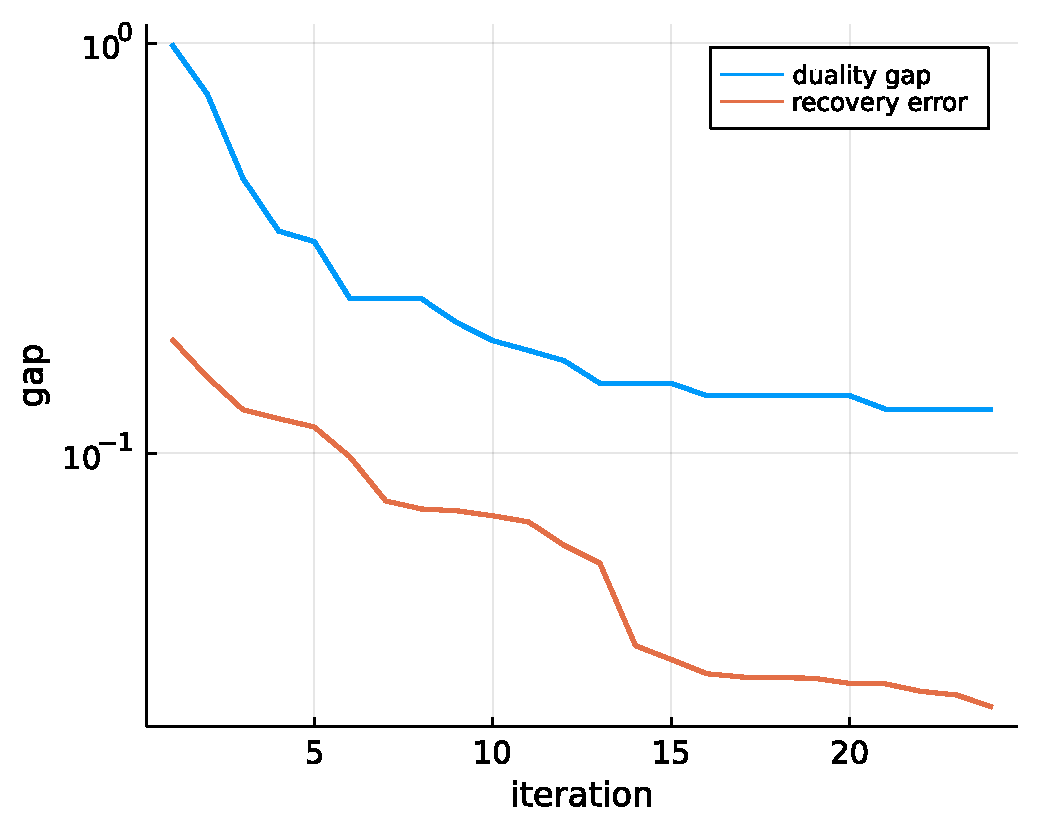
\includegraphics[width=.5\textwidth]{./figures/matrix_completion.pdf}
    \captionsetup{justification=centering}
    \caption{Matrix completion experiment.}
    \label{fig:matrix_completion}
\end{figure}

\subsection{Robust Principal Component Analysis} \label{sec:rpca}

\begin{figure}[t] \label{fig:rpca}
    \begin{subfigure}{.45\textwidth}
      \centering
      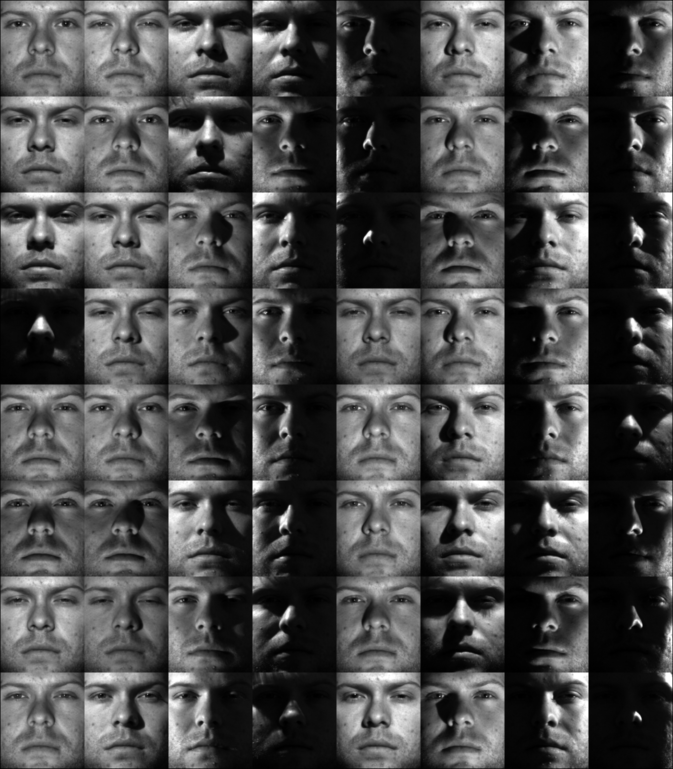
\includegraphics[width=\linewidth]{./figures/face.png}
      \captionsetup{justification=centering}
      \caption{Original faces.}
      \label{fig:face}
    \end{subfigure}
    \hfill
    \begin{subfigure}{.45\textwidth}
      \centering
      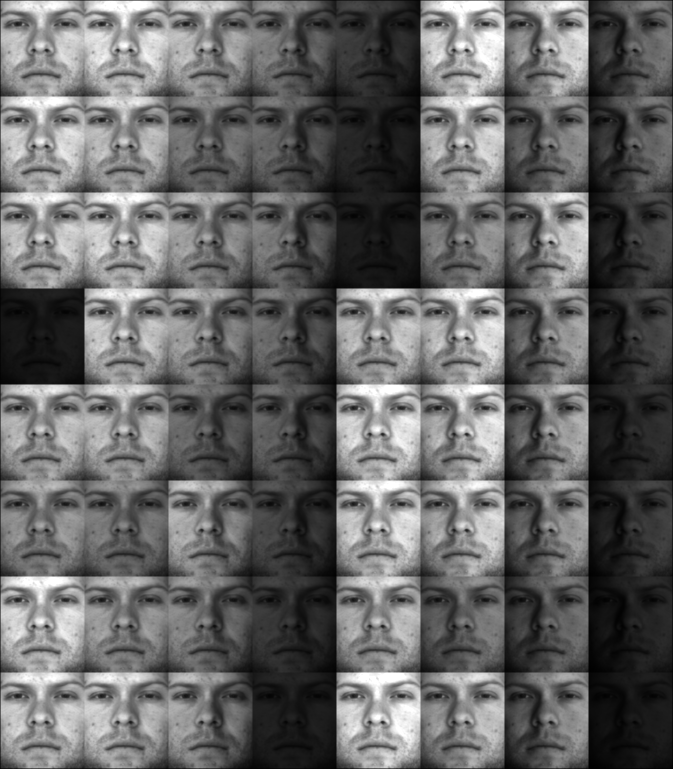
\includegraphics[width=\linewidth]{./figures/faceDeshadow.png}
      \captionsetup{justification=centering}
      \caption{Shadow-removed faces.}
      \label{fig:face_shadow}
    \end{subfigure}
    \captionsetup{justification=centering}
    \caption{Robust principal component analysis experiment.}
\end{figure}

In this section, we show that our primal-retrieval strategy can be applied to more complicated atomic sets besides polyhedral and spectral. We conduct the the similar experiment as in \cite{candes2011robust}. Face recognition algorithms are sensitive to shadows on faces. In order to obtain the best possible performance for these algorithms, it is desired to remove illumination variations and shadows on the face images. We obtained face images from the Yale B face database~\cite{georghiades2001few}. We show the original faces in \autoref{fig:face}, where each face image was of size $192\times 168$ with 64 different lighting conditions. The images were then reshaped into a matrix $M \in \Re^{32256 \times 64}$. Because of the similarity between faces and the sparse structure of the shadow, the matrix $M$ can be approximately decomposed into two components, i.e., 
\[M \approx L + S,\]
where $L$ is a low-rank matrix corresponding to the clean faces and $S$ is sparse matrix corresponding to the shadows. Based on the work by Fan et al.~\cite{fan2020polar}, we know that such decomposition can be obtained via solving the following convex optimization problem:
\begin{equation} \label{eq:rpca}
    \min_{L, S} \enspace \max\{\|L\|_*, \lambda \|S\|_1\}  \enspace \st  \enspace  \|L + S - M\| \leq \alpha.
\end{equation}
By \cite[Proposition~7.3]{fan2019alignment}, we know that \eqref{eq:rpca} is equivalent to 
\begin{equation} \label{eq:rpca2}
    \min_{x} \enspace \gauge\As(x)  \enspace \st  \enspace  \|x - M\| \leq \alpha,
\end{equation}
where $\Ascr = \lambda \Ascr_1 + \Ascr_2$, $\Ascr_1 = \{uv^T \mid u \in \mR^m,\ v \in \mR^n,\ \|u\|_2=\|v\|_2 = 1\}$ and $\Ascr_2 = \{\pm e_ie_j^T \mid i \in [m], j \in [n]\}$. The recovered low-rank component is shown in \autoref{fig:face_shadow}. As we can see from the figure, most of the shadow are successfully removed. This experiment suggests that our primal-retrieval technique can potentially be used for more complex atomic set and allow the underlying the dual-algorithm to produce satisfactory result within a reasonable number of iterations. 





\section{Proofs}

\subsection{Derivation of duals}\label{app:duals}

We derive the dual problems~\eqref{prob:dual1},~\eqref{prob:dual2} and~\eqref{prob:dual3} using the Fenchel\textendash Rockafellar duality framework. We use the following result.
\begin{theorem}[\protect{\cite[Corollary~31.2.1]{rockafellar1970convex}}]\label{thm-fenchel}
  Let $f_1:\Re^n\to\Re$ and $f_2:\Re^m\to\Re$ be two closed proper convex functions and let $M$ be a linear operator from $\Re^n$ to $\Re^m$, then
  \[\inf_{x \in \Re^n} f_1(x) + f_2(Mx) = \inf_{y \in \Re^m} f_1^*(M^*y) + f_2^*(-y).\]
  If there exist $x$ in the interior of $\dom f_1$ such that $Mx$ in the interior of $\dom f_2$, then strong duality holds, namely both infima are attained. 
\end{theorem}
We also need a result that describes the relationship between gauge, support, and indicator functions. 
\begin{proposition}[\protect{\cite[Proposition~3.2]{fan2019alignment}}] \label{prop-conjugate-gauge}
  Let $C\subset\Re^n$ be a closed convex set that contains the origin. Then 
  \[\gauge_C = \sigma_{C^\circ}=\delta_{C^\circ}^*.\]
\end{proposition}

For problem~\eqref{prob:primal1}, let
\[
  f_1 := \lambda\gauge\As \enspace\text{and}\enspace f_2 := f(b - \cdot)
\]
By the properties of conjugate functions and~\autoref{prop-conjugate-gauge}, we obtain 
\[
  f_1^* =  \delta_{(\frac{1}{\lambda}\Ascr)^\circ} = \delta_{\{x\mid \sigma\As(x)\leq\lambda\}} \enspace\text{and}\enspace f_2^* = \ip{b}{\cdot} + f^*(-\cdot).
\]
Then by~\autoref{thm-fenchel}, we can get the dual problem for~\eqref{prob:primal1} as
\[\minimize{y\in\Re^m} f^*(y) - \ip{b}{y} \enspace\text{subject to}\enspace \sigma\As(M^*y)\leq\lambda.\]

For~\eqref{prob:primal2},
\[f_1 = \delta_{\gauge\As\leq\tau} = \delta_{\tau\Ascr} \enspace\text{and}\enspace f_2 = f(b - \cdot).
\]
By the properties of conjugate functions and~\autoref{prop-conjugate-gauge}, we obtain 
\[f_1^* = \sigma_{\tau\Ascr} = \tau\sigma\As \enspace\text{and}\enspace f_2^* = \ip{b}{\cdot} + f^*(-\cdot).
\]
Then by~\autoref{thm-fenchel}, it follows that the dual problem for~\eqref{prob:primal2} is 
\[\minimize{y\in\Re^m} f^*(y) - \ip{b}{y} + \tau\sigma\As(M^*y).\]

For~\eqref{prob:primal3},
\[
  f_1 = \gauge\As \enspace\text{and}\enspace f_2 = \delta_{\{x\mid f(b - x)\leq\alpha\}}.
\]
By the properties of conjugate functions and~\autoref{prop-conjugate-gauge}, we can get that 
\[
  f_1^* = \delta_{\{x\mid \sigma\As(x)\leq1\}} \enspace\text{and}\enspace f_2^* = \sigma_{\{f(b - x)\leq\alpha\}}.\]
Then by~\cite[Example~E.2.5.3]{hiriart-urruty01}, we know that the support function of the sublevel set is 
\[f_2^* = \sigma_{\{x\mid f(b - x)\leq\alpha\}} = \min_{\beta > 0} \beta\left(f^*\left(-\frac{\cdot}{\beta}\right) + \alpha\right) + \ip{b}{\cdot}.\]
Finally, by~\autoref{thm-fenchel}, we can get the dual problem for~\eqref{prob:primal3} as
\[\minimize{y\in\Re^m,\ \beta > 0} \beta \left( f^*\left( \frac{y}{\beta} \right) + \alpha \right) - \ip{b}{y} \enspace \text{subject to}\enspace \sigma\As(M^* y) \leq 1.\]


\subsection{Proof of \autoref{thm:p0}} \label{app:main_proof}

The proof of this Theorem relies on the duality between smoothness and strong convexity.
\begin{lemma}[\protect{\cite[Theorem~6]{kakade2009duality}}] \label{lemma:conjugate}
   If $f$ is $L$-smooth, then $f^*$ is $\frac{1}{L}$-strongly convex.
\end{lemma}

\begin{proof}[Proof of Theorem~\ref{thm:p0}]
    \begin{itemize}
      \item[a)] Let $y^*$ denote the optimal dual variable for~\eqref{prob:dual1}. First, we show that $\|y - y^*\|$ can be bounded by the duality gap. Let $g(y) = f^*(y) - \ip{b}{y}$. By~\autoref{lemma:conjugate}, $f^*$ is $\frac{1}{L}$-strongly convex, and it follows that $g$ is also $\frac{1}{L}$-strongly convex. By the definition of strong convexity, 
      \[\forall s \in \partial g(y^*), \enspace g(y) \geq g(y^*) + \ip{s}{y- y^*} + \frac{1}{2L}\|y - y^*\|^2.
      \]
      Optimality requires that 
      \[\exists s \in \partial g(y^*), \enspace \ip{s}{y- y^*} \geq 0 \quad \forall y \enspace\text{s.t.}\enspace \sigma\As(M^*y)\leq\lambda.\]
      Therefore, by reordering the inequality,
      \begin{align}
         \|y - y^*\| & \leq \sqrt{2L(g(y) - g(y^*))}
         \quad \forall x \in \Re^n.
      \end{align} 
    
      Next, we show that $\Escr\As(M^*y^*) \subseteq \Escr\As(M^*y, \epsilon_1)$. For any $a \in \Escr\As(M^*y^*)$, 
      \begin{align*}
        \ip{a}{M^*y} &= \sigma\As(M^*y^*) + \ip{Ma}{y - y^*}
        \\&\geq \sigma\As(M^*y^*) - \left(\max\limits_{a \in \Ascr}\|Ma\|\right)\|y - y^*\|
        \\&\geq \sigma\As(M^*y^*) - \left(\max\limits_{a \in \Ascr}\|Ma\|\right)\sqrt{2L(g(y) - g(y^*))}
        \\&\geq \sigma\As(M^*y) - \epsilon_1,
      \end{align*}
      where the last inequality follows from the fact that $\sigma\As(M^*y^*) = \lambda$ and $y$ is feasible for \eqref{prob:dual3}. 
    
      \item[b)] Let $y^*$ denote the optimal dual variable for~\eqref{prob:dual2}. First, we show that $\|y - y^*\|$ can be bounded by the duality gap. Let $g(y) = f^*(y) - \ip{b}{y} + \tau\sigma\As(M^*y)$. By~\autoref{lemma:conjugate}, $f^*$ is $\frac{1}{L}$-strongly convex, and it follows that $g$ is also $\frac{1}{L}$-strongly convex. 
      By the definition of strongly convex, 
      \[\forall s \in \partial g(y^*), \enspace g(y) \geq g(y^*) + \ip{s}{y- y^*} + \frac{1}{2L}\|y - y^*\|^2.\]
      By optimality, $0 \in \partial g(y^*)$. Reorder the inequality to deduce that
      \[\|y - y^*\|_2 \leq \sqrt{2L(g(y) - g(y^*))}.\]
    
      Next, we show that $\Escr\As(M^*y^*) \subseteq \Escr\As(M^*y, \epsilon_2)$. For any $a \in \Escr\As(M^*y^*)$, 
      \begin{align*}
        \ip{a}{M^*y} &\geq \sigma\As(M^*y^*) - \left(\max\limits_{a \in \Ascr}\|Ma\|\right)\|y - y^*\|
        \\&= \sigma\As(M^*y) - \left(\sigma\As(M^*y) - \sigma\As(M^*y^*)\right) - \left(\max\limits_{a \in \Ascr}\|Ma\|\right)\|y - y^*\|
        \\&\geq \sigma\As(M^*y) - 2\left(\max\limits_{a \in \Ascr}\|Ma\|\right)\|y - y^*\|
        \\&\geq \sigma\As(M^*y) - \epsilon_2.
      \end{align*}
    
      \item[c)] Let $(y^*, \beta^*)$ denote the optimal dual variables for~\eqref{prob:dual3}. First, we show that $\|y - y^*\|$ can be bounded by the duality gap. Let 
      \[g(y) = \beta^*f^* \left(\frac{y}{\beta^*} \right) + \beta^*\alpha - \ip{b}{y}.\] 
      By~\autoref{lemma:conjugate}, $f^*$ is $\frac{1}{L}$-strongly convex, and it's not hard to check that $g$ is $\frac{1}{\beta^*L}$-strongly convex. By the definition of strongly convex,
      \[\forall s \in \partial g(y^*), \enspace g(y) \geq g(y^*) + \ip{s}{y- y^*} + \frac{1}{2\beta^*L}\|y - y^*\|^2.\]
      By optimality,
      \[\exists s \in \partial g(y^*), \enspace\ip{s}{y- y^*} \geq 0 \quad \forall y \enspace\text{s.t.}\enspace \sigma\As(M^*y)\leq1.\]
      Reorder the inequality to deduce that 
      \[\|y - y^*\|_2 \leq \sqrt{2\beta^*L(g(y) - g(y^*))}.\]
    %   \begin{align}
    %      \|y - y^*\|_2 & \leq \sqrt{2\beta^*L(g(y) - g(y^*))} \nonumber \\
    %      & \leq \sqrt{2\beta^*L \left(p_3(x) + d_3(y, \beta^*)\right) } \enspace \forall x \in \Re^n \text{s.t.} f(b - Mx)\leq\alpha\nonumber
    %      \\&\leq \sqrt{2\overline{\beta}L \left(p_3(x) + d_3(y, \beta^*)\right) } \enspace \forall x \in \Re^n \text{s.t.} f(b - Mx)\leq\alpha.
    %   \end{align} 
    
      Since $\beta^*$ is unknown to us, we will then get an upper bound for $d_3(y, \beta^*)$. Fix $y$, let $h(\beta) = d_3(y, \beta)$. By the property of perspective function, we know that $h$ is convex. Then it follows that 
      \[d_3(y, \beta^*) \leq \max\{d_3(y, \underline{\beta}), d_3(y, \overline{\beta})\}.\]
      Therefore,
      \[ \|y - y^*\|_2 \leq \sqrt{2\overline{\beta}L \left( \max\{d_3(y, \underline{\beta}), d_3(y, \overline{\beta})\} - d_3(y^*)\right) } .\]
    
      Finally, we show that $\Escr\As(M^*y^*) \subseteq \Escr\As(M^*y, \epsilon_3)$. For any $a \in \Escr\As(M^*y^*)$, 
      \begin{align*}
        \ip{a}{M^*y} &\geq \sigma\As(M^*y^*) - \left(\max\limits_{a \in \Ascr}\|Ma\|\right)\|y - y^*\|
        \\&= \sigma\As(M^*y) - \left(\sigma\As(M^*y) - \sigma\As(M^*y^*)\right) - \left(\max\limits_{a \in \Ascr}\|Ma\|\right)\|y - y^*\|
        \\&\geq \sigma\As(M^*y) - 2\left(\max\limits_{a \in \Ascr}\|Ma\|\right)\|y - y^*\|
        \\&\geq \sigma\As(M^*y) - \epsilon_3.
      \end{align*}
    \end{itemize}
\end{proof}


\subsection{Upper and lower bounds for \texorpdfstring{$\beta^*$}{} }
\label{app:bounds}
First, we consider~\eqref{prob:dual3}. Let $w = y/\beta$, then~\eqref{prob:dual3} can be equivalently expressed as 
\[\minimize{w} \inf_{\beta>0} \beta(f^*(w) - \ip{b}{w} + \alpha) \enspace\text{subject to}\enspace \sigma\As(M^* w) \leq \beta.\]
Fix $\beta = \beta^*$, then~\eqref{prob:dual3} can be expressed as 
\begin{equation} \label{prob:dual3equiv}
  \minimize{w} f^*(w) - \ip{b}{w} \enspace\text{subject to}\enspace \sigma\As(M^* w) \leq \beta^*.
\end{equation}
Now compare~\eqref{prob:dual3equiv} with~\eqref{prob:dual1} to conclude that they are equivalent when $\lambda = \beta^*$. It thus follows that~\eqref{prob:primal3} is equivalent to  
\begin{equation} \label{prob:p1beta}
    \minimize{x} f(b - Mx) + \beta^*\gauge\As(x). 
\end{equation}   

Next, consider using the level-set method~\cite{aravkin2016levelset} with bisection to solve~\eqref{prob:primal3}. There exists $\tau^* > 0$ such that~\eqref{prob:primal3} is equivalent to
\begin{equation} \label{prob:p2tau}
    \minimize{x} f(b - Mx) \enspace\text{subject to}\enspace \gauge\As(x)\leq\tau^*. 
\end{equation}
With the level-set method, we are able to get $(x_1, \tau_1)$ and $(x_2, \tau_2)$ such that $\tau_1 \leq \tau^* \leq \tau_2$ and $x_i$ is the optimum for 
\begin{equation} \label{prob:p2taui}
    \minimize{x} f(b - Mx) \enspace\text{subject to}\enspace \gauge\As(x)\leq\tau_i, 
\end{equation}
for $i = 1, 2$. Then there exits $\beta_1$ and $\beta_2$ such that $\beta_1 \geq \beta^* \geq \beta_2$ and $x_i$ is optimal for 
\begin{equation} \label{prob:p1betai}
    \minimize{x} f(b - Mx) + \beta_i\gauge\As(x),
\end{equation}
for $i = 1, 2$.

Finally, by~\cite[Theorem~5.1]{fan2019alignment} we can conclude that 
\[\beta_i = \sigma\As(M^*\nabla f(b - Mx_i)) \text{for} i = 1,2.\]
Therefore, we can get upper and lower bounds for $\beta^*$ via level-set method with bisection. Moreover, by strong duality and convergence of the bisection method, the gap between $\beta_1$ and $\beta_2$ will converge to zero. 

\subsection{Proof of Proposition~\ref{prop:polyhedral}}
\label{app:prop_proof}
\begin{proof}
  First, we show that for any $y_i$ such that $\| y_i - y_i^* \| \leq \frac{\delta}{4\| M \|_\Ascr}$, the condition 
  \[\Face\As( M^* y_i^*) \subseteq \texttt{EssCone}(\Ascr, M, y_i, k)\]
  holds. By \autoref{ass:blanket} and the definition of $\delta$-nondegeneracy, we know that 
  \begin{equation} \label{eq:Aprime}
  \begin{split}
    |  \Face\As( M^* y_i^*) | &= k \text{and} \\
    \langle Ma, y_i^* \rangle &\leq \sigma_{\Ascr}( M^* y_i^* ) - \delta \quad \forall a \notin \Face\As( M^* y_i^*).
  \end{split}
  \end{equation}
  For any $a \in \Face\As( M^* y_i^*)$, we have
  \begin{align*}
      & \langle a, M^* y_i \rangle \\
      \geq~& \langle a, M^* y_i^* \rangle - | \langle M a, y_i^* - y_i \rangle | \\
      \geq~& \sigma_{\Ascr}( M^* y_i^* ) - \| M \|_\Ascr \frac{\delta}{4\|M\|_{\Ascr}} \\
      \geq~& \sigma_{\Ascr}( M^* y_i^* ) - \frac{\delta}{4}.
  \end{align*}
  For any $a' \notin \Face\As( M^* y_i^*)$, we have 
  \begin{align*}
      & \langle a', M^* y_i \rangle \\
      \leq~ & \langle a', M^* y_i^* \rangle + | \langle M a', y_i^* - y_i \rangle | \\
      \leq~ & \langle a', M^* y_i^* \rangle + \frac{\delta}{4} \\
      \leq~ & \sigma_{\Ascr}( M^* y_i^* ) - \delta + \frac{\delta}{4} \quad \text{(By \eqref{eq:Aprime})} \\
      =~& \sigma_{\Ascr}( M^* y_i^* ) - \frac{3\delta}{4}.
  \end{align*}
    Therefore, 
    \begin{align*}
        \langle a, M^* y_i \rangle > \langle a', M^* y_i \rangle  \quad \forall a \in \Face\As( M^* y_i^*) \text{and} a' \notin \Face\As( M^* y_i^*).
    \end{align*}
    Notice that $\texttt{EssCone}(\Ascr, M, y_i, k)$ contains only the atoms that corresponds to the $k$ largest $\langle a, M^* y_i \rangle$. Therefore $\Face\As( M^* y_i^*) \subseteq \texttt{EssCone}(\Ascr, M, y_i, k)$.
    
    By the assumption $y_i^{(t)} \to y_i^*$. For $i \in \{1,2,3\}$, we know there exist $T_i > 0$ such that $\| y_i^{(t)} - y_i^* \| < \frac{\delta}{4\| M \|_\Ascr}$ for all $t > T$. Therefore 
    \[\Face\As( M^* y_i^*) \subseteq \texttt{EssCone}(\Ascr, M, y_i^{(t)}, k)~~\forall t > T\] 
    and we complete the proof.
\end{proof}

\subsection{Proof for \autoref{thm:svd_approx_score}}
\begin{proof}
  By the definition of $\rho(\cdot, \cdot)$, it follows that
  \[
    \rho(A, C) \leq \rho(B, C) \quad \forall A, B, C \subseteq \mR^{n \times m} ~\text{such that}~ A \subseteq B.
  \]
  We know that $ \Face\As( M^* y^* ) \subseteq  \Face\As( M^* y, \epsilon )$, then obviously we have 
  \[
    \rho( \Face\As( M^* y^* ), \widehat{\Ascr}  ) \leq \rho( \Face\As( M^* y, \epsilon ), \widehat{\Ascr}  ).
  \]
  For any $\Ascr_1, \Ascr_2 \subseteq \Ascr$,
  \begin{align}
    \rho( \Ascr_1, \Ascr_2 ) = \sqrt{ \adjustlimits\sup_{a_1 \in \Ascr_1} \inf_{a_2 \in \Ascr_2} \| a_1 - a_2 \|_F^2 } = \sqrt{ 2 - 2 \left( \adjustlimits \inf_{a_1 \in \Ascr_1} \sup_{a_2 \in \Ascr_2} \ip{a_1}{a_2} \right) }, \label{eq:norm2ip}
  \end{align}
  where the second equality holds since $\| a_1 \|_F = \| a_2 \|_F = 1$ by the definition of $\Ascr$. Define $\Ascr_1 = \Face\As( M^* y, \epsilon )$ and $\Ascr_2 = \widehat{\Ascr} = \{ U_r p q^T V_r^T | \|p\|_2 = \|q\|_2 = 1 \}$, where $U_r, V_r$ are the top-$r$ singular vectors of $M^*y$. Let $k \coloneqq \min\{n,m\}$, $\Cscr_1 = \{(p, q) \mid \sum_{i=1}^{k} \sigma_i p_i q_i \geq \sigma_1 - \epsilon,~ \|p\|_2 = \|q\|_2 = 1, ~p,q \in \mR^{ k }\}$ and $\Cscr_2 = \{(\hat{p}, \hat{q}) \mid \|\hat{p}\|_2 = \|\hat{q}\|_2 = 1, ~\hat{p},\hat{q} \in \mR^{ k }\}$, then
  \begin{align}
    \rho( \Ascr_1, \Ascr_2  ) & = \sqrt{ 2 - 2 \left( \min_{p, q \in \Cscr_1} \max_{ \hat{p}, \hat{q} \in \Cscr_2} \ip{ Up q^T V^T }{ U_r \hat{p} \hat{q}^T V_r^T } \right) } \nonumber \\
    & = \sqrt{ 2 - 2 \left( \min_{p, q \in \Cscr_1} \max_{ \hat{p}, \hat{q} \in \Cscr_2} \left( \sum_{i=1}^r p_i \hat{p}_i \right) \left( \sum_{i=1}^r q_i \hat{q}_i \right) \right) } \nonumber \\
    & = \sqrt{ 2 - 2 \left(\min_{p, q \in \Cscr_1} \| p_{1:r} \|_2 \| q_{1:r} \|_2 \right) } \label{eq:rho_exp} 
    % \text{subject to} & \sum_{i=1}^{k} \sigma_i p_i q_i \geq \sigma_1 - \epsilon,~ \|p\|_2 = \|q\|_2 = 1, ~p,q \in \mR^{ k }, \nonumber \\
  \end{align}
  Now we consider the subproblem in \eqref{eq:rho_exp}: 
  \begin{align}
    \min_{p,q}\enspace & \| p_{1:r} \|_2 \| q_{1:r} \|_2 \label{eq:reduced_p1} \tag{P$_1$} \\
    \text{subject to} & \sum_{i=1}^{k} \sigma_i p_i q_i \geq \sigma_1 - \epsilon,~ \|p\|_2 = \|q\|_2 = 1, ~p,q \in \mR^{ k }. \nonumber
  \end{align}
  If $p^*$ and $q^*$ is a solution of the problem \eqref{eq:reduced_p1}, then it's easy to verify that 
  \begin{align*}
    & \tilde{p} = \left[ \| p^*_{1:r} \|_2, 0,\ldots, \|p^*_{r+1:k}\|_2, 0, \ldots, 0 \right] \\ 
    \text{and} ~& \tilde{q} = \left[ \| q^*_{1:r} \|_2, 0,\ldots, \|q^*_{r+1:k}\|_2, 0, \ldots, 0 \right]
  \end{align*}
  is also a valid solution. Therefore there must exist solution $p^*, q^*$ such that $p_i = q_i = 0~\forall i \notin \{1, r+1\}$, that is only $p^*_1, q^*_1$ and $p^*_{r+1}$ and $q^*_{r+1}$ are greater or equal than 0. This allow us to further reduce the problem to
  \begin{align*}
    \min_{ p_1, q_1, p_{r+1}, q_{r+1} } &~  p_1 q_1 \\
    \text{subject to} & \sigma_1 p_1 q_1 + \sigma_{r+1} p_{r+1} q_{r+1} \geq \sigma_1 - \epsilon, \\
    & p_1^2 + p_{r+1}^2 = q_1^2 + q_{r+1}^2 = 1, ~p_1, q_1, p_{r+1}, q_{r+1} \geq 0. 
  \end{align*}
  It's easy to verify that when $\sigma_1 - \sigma_{r+1} \geq \epsilon$, the above problem attains solution at 
  \[
    p_1 = q_1 = \sqrt{\frac{\sigma_1 - \sigma_{r+1} - \epsilon}{ \sigma_1 - \sigma_{r+1} } } \text{and} p_{r+1} = q_{r+1} = \sqrt{1 - p_1^2}.
  \]
  When $\sigma_1 - \sigma_{r+1} < \epsilon$, the solution is simply $p_1 = q_1 = 0, p_{r+1}= q_{r+1} = 1$.
  Therefore the optimal value of \eqref{eq:reduced_p1} is $\max\{1 - \epsilon / ( \sigma_1 - \sigma_{r+1} ), 0\}$, plug this into \eqref{eq:rho_exp} and the proof is finished. 
\end{proof}

\begin{proposition}[Hausdorff error bound] \label{prop:dist_to_sol}
    Given $\widehat{\Ascr} \subseteq \Ascr$ such that , there exists $ x \in \cone ( \widehat{\Ascr} ) $ such that 
    \begin{equation}
            \| x - x^* \|_F \leq \dist( \suppa(x^*), \widehat{\Ascr} )\cdot \sqrt{| \suppa(x^*) |} \cdot \| x^* \|_F.  \label{eq:dist_to_sol}
    \end{equation}
\end{proposition}

\subsection{Proof of \autoref{prop:spectral}}
\begin{proof}
  By \autoref{prop:dist_to_sol}, we know that there exist $\tilde{x}$ satisfies \eqref{eq:dist_to_sol}.
  Then by the $L$-smoothness of $f$,
  \begin{align}
      f( b - M \tilde{x} ) &~\leq~ f( b - M x^* ) + \langle \nabla f( b - M x^* ), M( x^* - \tilde{x} ) \rangle + \frac{L}{2} \| M( x^* - \tilde{x} ) \|^2  \nonumber \\
      &~\leq~ f( b - M x^* ) + \| \nabla f( b - M x^* ) \| \| M( x^* - \tilde{x} ) \| + \frac{L}{2} \| M( x^* - \tilde{x} ) \|^2. \label{eq:errorBoundIntermediate1}
  \end{align}
  By the smoothness and convexity of $f$, we further have
  \begin{align*}
      \| \nabla f( b - M x^* ) - \nabla f(0) \|^2 \leq 2L ( f(b - M x^*) - f(0) ).
  \end{align*}
  Note that $f(0)$ and $\nabla f(0) = 0$, the above reduces to $\| \nabla f( b - M x^* ) \| \leq \sqrt{2 L \alpha}$. Combining with \eqref{eq:errorBoundIntermediate1}, we obtain
  \begin{align*}
      f( b - M \tilde{x} ) &~\leq~ f( b - M x^* ) + \sqrt{2 L \alpha} \| M( x^* - \tilde{x} ) \| + \frac{L}{2} \| M( x^* - \tilde{x} ) \|^2 \\
      &~\leq~ f( b - M x^* ) + \sqrt{2 L \alpha} \| M \| \rho( \suppa(x^*), \widehat{\Ascr} )\cdot \sqrt{| \suppa(x^*) |} \cdot \| x^* \|_F  \\
      &\qquad + \frac{L}{2} \rho( \suppa(x^*), \widehat{\Ascr} )^2 | \suppa(x^*) | \| x^* \|_F^2.
  \end{align*}
\end{proof}


























%    5. AtomicOpt.jl: a Julia package for structured optimization
%% The following is a directive for TeXShop to indicate the main file
%%!TEX root = diss.tex
\chapter{AtomicOpt.jl: a Julia package for structured optimiztaion}
\label{ch:App-AtomicOpt}

\section{Introduction} \label{sec:5-1}
In this chapter, we introduce a open-source Julia package \texttt{AtomicOpt.jl}\footnote{\url{https://github.com/MPF-Optimization-Laboratory/AtomicOpt.jl}} for solving a class of structured optimization problems. All the numerical experiments in \autoref{ch:Dual-Struc-Opt}, \autoref{ch:App-Sig-Demix} and \autoref{ch:App-Primal-Retrieval} are conducted using this package. 

\texttt{AtomicOpt.jl} aims to solve the following cardinality-constrained problem:
\begin{equation} \label{eq:main_prob_atomic_opt} 
\begin{split}
  \find & x_1, \dots, x_k \in \Re^n \\
  \sut  & \left\|M\left(\sum_{i=1}^k x_i\right) - b \right\| \leq \alpha \tand \\
        & \card\Asi(x_i) \leq r_i \enspace \forall i \in [k],
\end{split}
\end{equation}
where $m, n, k, r_i ~\forall i\in[k]$ are positive integers, $\alpha$ is a positive scalar indicating the constraint on the data-fitting term, $M: \Re^n \to \Re^m$ is a linear operator with $m < n$, $b \in \Re^m$ is the observation vector, $\Ascr_i \subseteq \Re^n$ is the basic atomic set for any $i\in[k]$ such that the set of exposed atoms $\Escr\Asi$ \eqref{eq:exposed-atoms} can be efficiently found, and $\card\As$ is the cardinality function as defined in \eqref{eq-card-fcn}. 

The signal demixing problem introduced in \autoref{ch:App-Sig-Demix} can be expressed in the format of problem \eqref{eq:main_prob_atomic_opt}, which can be viewed as a generalized version of the problem \eqref{eq:main_prob} introduced in \autoref{ch:App-Primal-Retrieval}. 

As we introduced in \autoref{ch:App-Sig-Demix}, in practice, we can solve the convex relaxation to the problem \eqref{eq:main_prob_atomic_opt}. More specifically, we know that under mild conditions, the following assumption holds. 
\begin{assumption} \label{ass:atomic_opt}
There exist positive scalars $\lambda_i, i\in[k]$, such that the minimizers $\{x_i^*\}_{i=1}^k$ to the following structured optimization problem
\begin{equation} \label{eq:main_prob_atomic_opt_cvx} 
  \begin{split}
      x_1^*, \dots, x_k^* &\in \argmin{x_1, \dots, x_k \in \Re^n} \max_{i=1,\dots,k} \enspace \frac{1}{\lambda_i}\gauge\Asi(x_i) \sut \sum_{i=1}^k x_i = x^* \text{where}\\
      x^* &\in \argmin{x\in\Re^n} \gauge\As(x) \sut \|Mx- b\| \leq \alpha \text{with} \\
      \Ascr &\coloneqq \sum_{i=1}^k \lambda_i\Ascr_i
  \end{split}
\end{equation}
are feasible to problem \eqref{eq:main_prob_atomic_opt}. 
\end{assumption}

As we introduced in \autoref{ch:App-Primal-Retrieval}, for better space complexity, we can instead solve the following dual formulation to the problem \eqref{eq:main_prob_atomic_opt_cvx}:
\begin{equation} \label{eq:main_prob_atomic_opt_dual} 
    \min_{r\in\Re^m}\enspace \gauge\MAs(b-r) \sut \|r\| \leq \alpha.
\end{equation}
Then near-feasible solutions to problem \eqref{eq:main_prob_atomic_opt} can obtained via \autoref{alg:primal_recover}. 

We describe the whole procedure and the candidate algorithms in \autoref{sec:5-2}. Then in \autoref{sec:5-3}, we introduce the basic atomic sets we include in this package. Finally, we show some examples using \texttt{AtomicOpt.jl}. 


\section{Algorithms} \label{sec:5-2}

In this section, we describe a procedure for obtaining near-feasible solutions to problem \eqref{eq:main_prob_atomic_opt}. The procedure first solves the dual formulation \eqref{eq:main_prob_atomic_opt_dual} using an algorithm requiring only the storage of several vectors of length $m$, which represents the size of the data $b$. The algorithm depends on the level-set method \cite{berg2011sparse,berg2008probing} and a generalized version of the dual conditional gradient method (\autoref{algo:dual-conditional-gradient}), which we describe in \autoref{sec:level} and \autoref{sec:dcg} respectively. As we show in \autoref{sec:primal_retrieval}, the solutions to the problem \eqref{eq:main_prob_atomic_opt} is subsequently obtained via an unconstrained linear least-squares problem that uses information implicit in the dual vector. \autoref{alg-level-set} summarizes the overall procedure. 

\begin{algorithm}[t]
  \DontPrintSemicolon
  \SetKwComment{tcp}{\tiny [}{]}
  \caption{Main procedure implemented in \texttt{AtomicOpt.jl}.\label{alg-level-set}}
  \smallskip
  \KwIn{noise level $\alpha>0$; accuracy $\epsilon>0$}
  $\tau^{0} \gets 0$
 
  \For(\tcp*[f]{\tiny level-set iterations}){\nllabel{alg-level-set-loop}$t\gets0,1,2,\ldots$}{
    $(r\t,\, p\t,\, \ell\t)\leftarrow\texttt{DCG}(\tau\t)$ \tcp*{\tiny solve~\eqref{eq:value-fn} approximately}\nllabel{alg-level-set-cg}
    \lIf(\tcp*[f]{\tiny test $\epsilon$-infeasibility}){$\|r\t\| \leq \alpha + \epsilon$}{break}
    $\tau\tp1 \gets \tau\t + \frac{\ell\t-\alpha^2/2}{\ip{p\t}{r\t}}$\nllabel{alg-level-set-update}
    \tcp*{\tiny Newton update}
  }
   $(x_1,\ldots,x_k) \gets \mbox{solve~\eqref{eq:primal-recovery}}$ \nllabel{alg-primal-recovery}
   \tcp*{\tiny primal retrieval}
  \Return{$(x_1,\ldots,x_k)$}
 \end{algorithm}


\subsection{Level-set method} \label{sec:level}
The loop beginning at \autoref{alg-level-set-loop}  of \autoref{alg-level-set} describes the level-set method \cite{BergFriedlander:2008,berg2011sparse,aravkin2016levelset} for solving problem \eqref{eq:main_prob_atomic_opt_dual}. More specifically, it approximately solves a sequence of problems
\begin{equation} \label{eq:value-fn}
  v(\tau) \coloneqq \min_{r}\left\{\frac{1}{2}\|r\|^2 ~\big\vert~ \gauge\MAs(b-r) \leq \tau\right\}. 
\end{equation} 
parameterized by the scalar $\tau$ that defines the level-set constraint, which is also known as the value function. The level-set method constructs a monotonically-increasing sequence $\{\tau\t\}$ that converges to the leftmost root $\tau^*$ of the equation $v(\tau) = \half\alpha^2$,
which represents the fidelity constraint of problem~\eqref{eq:main_prob_atomic_opt_dual}. Under modest assumptions satisfied by this problem, the sequence $\tau\t\to\tau^*=\opt$, the optimal value of~\eqref{eq:main_prob_atomic_opt_dual}. Let $r_{\tau}$ denote the minimizer for $v(\tau)$, then for any $\tau \leq \tau^*$ satisfying $v(\tau) \leq (\alpha+\epsilon)^2/2$, $r_\tau$ is a super-optimal and $\epsilon$-feasible solution to~\eqref{eq:main_prob_atomic_opt_dual}, i.e., a solution $r$ satisfies 
\begin{equation} \label{eq:super-optimal}
  \gauge\MAs(b-r) \leq \opt \text{and} \|r\| \leq \alpha + \epsilon,
\end{equation}
where $\epsilon$ is a specified optimality tolerance. 

The level-set algorithm requires $\BigOh(\log(1/\epsilon))$ approximate evaluations of the optimization problem~\eqref{eq:value-fn} to achieve this optimality condition. Each approximate evaluation provides a global lower-minorant of $v$ that is used by a Newton-like update to the level-set parameter $\tau\t$; see line~\ref{alg-level-set-update}. An illustration of the idea of the level-set method is shown in~\autoref{fig:value_fn}. 

\begin{figure}[t] 
    \begin{subfigure}{.48\textwidth}
      \centering
      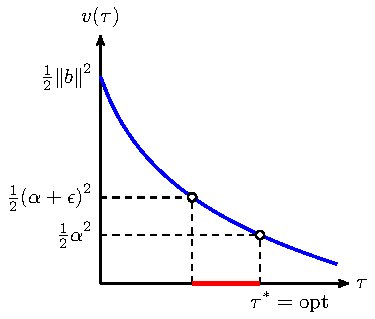
\includegraphics[width=\linewidth, page=1]{./figures/illustrations3}
      \captionsetup{justification=centering}
      \caption{Value function.}
    \end{subfigure}
    \hfill
    \begin{subfigure}{.48\textwidth}
      \centering
      \includegraphics[width=\linewidth, page=2]{./figures/illustrations3}
      \captionsetup{justification=centering}
      \caption{Newton-like update.}
    \end{subfigure}
    \captionsetup{justification=centering}
    \caption{Illustration of the level-set method.}
    \label{fig:value_fn}
\end{figure}

\subsection{Dual conditional gradient method} \label{sec:dcg}

\begin{algorithm}[t]
  \DontPrintSemicolon
  \setcounter{AlgoLine}{0}
  \SetKwComment{tcp}{\tiny [}{\tiny ]}
  \caption{Generalized dual conditional gradient method: \texttt{DCG}($\tau$). \label{alg:dcg}}
  \KwIn{$\tau$}

  $r^{(0)} \gets b$;\ $q_i^{(0)} \gets 0$ for all $i\in[k]$\;

  \For{$t\gets0,1,2,\ldots$}{
     $p_i\t \in \tau\lambda_i\Escr(M\Ascr_i;\,r\t)$ for all $i\in[k]$\tcp*{\tiny expose atoms}\nllabel{algo-expose-atom}
     $\Delta r_i\t\gets p_i\t-q_i\t$ for all $i\in[k]$\tcp*{\tiny compute $\Delta r$}
     $\rho\t \gets \ip{r\t}{\sum_{i=1}^k\Delta r_i\t}$\tcp*{\tiny optimality gap}
     \lIf(\tcp*[f]{\tiny break if optimal}){$\rho\t<\epsilon$}{
       break
     }
     $(\theta_1\t, \dots, \theta_k\t) \gets \mbox{solve~\eqref{eq:line_search}}$\tcp*{\tiny exact linesearch}\nllabel{algo-line-search}
     $r\tp1 \gets r\t - \sum_{i=1}^k \theta_i\Delta r_i\t$\tcp*{\tiny update $r$}
     $q_i\tp1 \gets q_i\t+\theta_i\t\Delta r_i\t$ for all $i\in[k]$\tcp*{\tiny update $q$}
  }
  $\ell\t\gets\half\|r\t\|^2-\rho\t$\tcp*{\tiny lower bound on optimal value}

  \Return{$r\t$, $\sum_{i=1}^k p_i\t$, $\ell\t$}
\end{algorithm}

The level-set subproblems are solved approximately using the generalized dual conditional-gradient method described by \autoref{alg:dcg}, which is generalized version of \autoref{algo:dual-conditional-gradient}. The main computational cost are in \autoref{algo-expose-atom} and \autoref{algo-line-search}. 

In \autoref{algo-expose-atom}, we use $r\t$ to expose atoms from $M\Ascr_i$, which can be implemented in parallel using the following identity, i.e.,
\begin{equation*}
  \Escr(M\Ascr_i;\,r\t) \equiv M\cdot\Escr(\Ascr_i, M^*r\t).
\end{equation*}
Recall that $\Ascr_i$ is the basic atomic set, so $\Escr(\Ascr_i, M^*r\t)$ can be efficiently computed. This formulation is convenient in cases where the operator $M$ can be applied implicitly to elements of the atomic set $\Ascr_i$. 

\autoref{algo-line-search} exhibits the exact linesearch, i.e., it solves the following box-constrained optimization problem
\begin{equation} \label{eq:line_search}
  \min_{\theta_1, \dots, \theta_k \in [0,1]} \enspace \left\|r\t - \sum_{i=1}^k \theta_i\Delta r_i\t\right\|.
\end{equation}
The exact linesearch problem \eqref{eq:line_search} is solved by using \texttt{LBFGSB.jl}\footnote{\url{https://github.com/Gnimuc/LBFGSB.jl}}, which is a Julia wrapper for the L-BFGSB-B algorithm developed by~\citet{zhu1997algorithm}. 

The conditional-gradient method converges to the required optimality within $\BigOh(1/\epsilon)$ iterations \cite{jaggi2013revisiting}. Combined with the complexity of the level-set method, we thus expect a total worst-case complexity of $\BigOh(\log(1/\epsilon)/\epsilon)$ iterations to satisfy the optimality condition~\eqref{eq:super-optimal}.

\subsection{Primal retrieval} \label{sec:primal_retrieval}
Once \autoref{alg-level-set} reaches \autoref{alg-primal-recovery}, the vector $r\t$ contains information about the atoms that are in the support of each of minimizers $x_i^*$ to the problem \eqref{eq:main_prob_atomic_opt_cvx}; cf. \autoref{th:polar-alignment}. According the result developed in \autoref{ch:App-Primal-Retrieval}, we can then obtain near-feasible solutions to the original cardinality-constrained problem \eqref{eq:main_prob_atomic_opt} via solving the following constrained optimization problem
\begin{equation} \label{eq:primal-recovery}
  \min_{x_1, \dots, x_k \in \Re^n} \enspace \left\|b - M\sum_{i=1}^k x_i\right\| \st x_i \in \texttt{EssCone}_{\Ascr_i, M, k_i}(r\t),
\end{equation}
where $\texttt{EssCone}$ is defined as in \eqref{eq:ess_cone}. The primal-retrieval problem \eqref{eq:primal-recovery} is solved by using \texttt{IterativeSolvers.jl}\footnote{\url{https://github.com/JuliaLinearAlgebra/IterativeSolvers.jl}}, which provides a Julia wrapper for the well-known conjugate gradient method.  



\section{Basic atomic sets} \label{sec:5-3}

In this section, we introduce some basic atomic sets implemented in \texttt{AtomicOpt.jl}. 

\paragraph{\texttt{OneBall}} refers to the atomic set described in \autoref{example-one-norm}. The basic usage is shown in the following code block. 
\begin{code}
  using AtomicOpt
  using LinearAlgebra
  using Test
  # set dimension
  n = 10
  # construct atomic set 
  A = OneBall(n)
  # generate random vector
  z = randn(n)
  # expose atom
  a = expose(A, z)
  # test
  @test dot(a,z) ≈ support(A, z)
\end{code}

\paragraph{\texttt{NucBall}} refers to the atomic set described in \autoref{example-nuclear-norm}. The basic usage is shown in the following code block. 
\begin{code}
  using AtomicOpt
  using LinearAlgebra
  using Test
  # set dimension
  n1, n2 = 10, 15
  # construct atomic set 
  A = NucBall(n1, n2)
  # generate random matrix
  z = randn(n1, n2)
  # expose atom
  a = expose(A, z)
  # test
  @test dot(a,z) ≈ support(A, z)
\end{code}

\paragraph{\texttt{TraceBall}} refers to the atomic set described in \autoref{example-trace-norm}. The basic usage is shown in the following code block. 
\begin{code}
  using AtomicOpt
  using LinearAlgebra
  using Test
  # set dimension
  n = 10
  # construct atomic set 
  A = TraceBall(n)
  # generate random matrix
  z = randn(n, n)
  # expose atom
  a = expose(A, z)
  # test
  @test dot(a,z) ≈ support(A, z)
\end{code}

\paragraph{\texttt{BlkNucBall}} refers to the atomic set described in \autoref{sec:3-5-4}. The basic usage is shown in the following code block. 
\begin{code}
  using AtomicOpt
  using LinearAlgebra
  using Test
  # set dimension
  n, bn = 10, 2
  # construct atomic set 
  A = BlkNucBall(n, n, bn, bn)
  # generate random matrix
  z = randn(n, n)
  # expose atom
  a = expose(A, z)
  # test
  @test dot(a,z) ≈ support(A, z)
\end{code}


\section{Examples} \label{sec:5-4}

In this section, we show how to use \texttt{AtomicOpt.jl} to solve some structured optimization problems introduced in \autoref{ch:Dual-Struc-Opt}, \autoref{ch:App-Sig-Demix} and \autoref{ch:App-Primal-Retrieval}. For simplicity, for the examples here we will use synthetic data. More examples with real data can be found on the GitHub page. 

\paragraph{Basis pursuit denoise} refers to the problem introduced in \autoref{ex:bpdn}. The following code block summarizes how to solve this problem using \texttt{AtomicOpt.jl}.
\begin{code}
  using AtomicOpt
  using LinearAlgebra
  using Printf
  import Random: seed!, randperm
  # set dimensions
  m, n, k = 2^8, 2^10, 8
  # random measurement operator
  M = randn(m, n) 
  # ground-truth signal with nnz = k
  p = randperm(n); p = p[1:k]; 
  x0 = zeros(n); x0[p] = randn(k)
  # noise
  η = randn(m)/100
  # measurement
  b = M*x0 + η
  # atomic set
  A = OneBall(n; maxrank=k)
  # solve the basis pursuit denoise problem
  sol = level_set(M, b, A, α = norm(η))
  # construct primal solution
  x = constructPrimal(sol)
  # report error
  @printf("relative difference between x0 and x: .2%f", norm(x - x0)/norm(x0))
\end{code}

\paragraph{Low-rank matrix completion} refers to the problem introduced in \autoref{ex:mc}. The following code block summarizes how to solve this problem using \texttt{AtomicOpt.jl}.
\begin{code}
  using AtomicOpt
  using LinearAlgebra
  using SparseArrays
  using Printf
  import Random: seed!, randperm
  # generate a random m×n matrix with rank r
  m, n, r = 100, 100, 3 
  X = rand(m, n)
  U, S, V = svd(X)
  X0 = U[:,1:r] * Diagonal( S[1:r] ) * V[:,1:r]'
  # generate a random mask with nnz ≈ m*n*p
  p = 0.5
  mask = sprand(Bool, m, n, p); 
  mask = convert(SparseMatrixCSC{Float64, Int64}, mask)
  # measurement
  B =  mask .* X0
  b =  B.nzval
  # operator
  Mop = MaskOP(mask)
  # atomic set
  A = NucBall(m, n, r)
  # solve the matrix completion problem
  sol = level_set(M, b, A, α = 0.0)
  # construct primal variable
  x = constructPrimal(sol)
  X = reshape(x, m, n)
  # Report recovery error
  @printf("relative difference between X0 and X: .2%f", norm(X - X0)/norm(X0))
\end{code}

\paragraph{Sparse and low rank matrix decomposition} refers to the problem introduced in \autoref{sec:3-5-3}. The following code block summarizes how to solve this problem using \texttt{AtomicOpt.jl}.
\begin{code}
  using AtomicOpt
  using LinearAlgebra
  using SparseArrays
  using Printf
  import Random: seed!, randperm
  # generate a random m×n matrix with rank r
  m, n, r = 100, 100, 3 
  X = rand(m, n)
  U, S, V = svd(X)
  x1 = U[:,1:r] * Diagonal( S[1:r] ) * V[:,1:r]'
  # generate a random m*n matrix with nnz ≈ m*n*p
  p = 0.01
  x2 = randn(m, n) .* sprand(Bool, m, n, p)
  k = nnz(x2)
  # measurement
  b = vec(x1 + x2)
  # atomic set
  A1 = NucBall(m, n, maxrank=r); A1 *= gauge(A1, xl)
  A2 = OneBall(m*n, maxrank=k); A2 *= gauge(A2, xs)
  A = A1 + A2
  # solve the sparse and low-rank decomposition problem
  sol = level_set(I(m*n), b, A, α = 0.0)
  # construct primal variable
  x = constructPrimal(sol)
  # Report recovery error
  @printf("relative difference for x1: .2%f", norm(x1 - x[1])/norm(x1))
  @printf("relative difference for x2: .2%f", norm(x2 - x[2])/norm(x2))
\end{code}


\section{Discussion} \label{sec:5-5} 
\texttt{AtomicOpt.jl} provides not only a solver but also a framework for structured optimization. You can easily add new basic atomic sets to it, as long as you know how to implement the expose operation. 










\part{Federated optimization}

%    6. FedDCD: a dual approach for federated optimization
%% The following is a directive for TeXShop to indicate the main file
%%!TEX root = diss.tex
\chapter{Duality in federated optimization}
\label{ch:Dual-Fed-Opt}

\part{Application of structured optimization in federated learning}

%    7. Fair data valuation in horizontal federated learning
%% The following is a directive for TeXShop to indicate the main file
%%!TEX root = diss.tex
\chapter{Fair data valuation in horizontal federated learning}
\label{ch:Val-HFL}

\section{Introduction} \label{sec:7.1}

Building large and powerful machine learning models often needs large amounts of training data. In many industry-scale applications, training data is distributed in the form of silos, that is, training data is obtained and maintained by many data owners instead of being centralized at the place of a single owner or a data center. Because of industrial competition, privacy concerns, legal restrictions, and many other possible reasons, integrating or centralizing data from different sources faces enormous resistance and is often even infeasible. Federated learning~\cite{federated2016} is promising for training machine learning models on distributed data sources. It facilitates collaboration among a group of data owners (aka.~``clients'') and, at the same time, preserves their privacy. The central idea of federated learning is to periodically aggregate local models from clients to produce a more general and capable global model.

Federated learning can be divided into two classes: horizontal federated learning and vertical federated learning~\cite{yang2019federated}. Horizontal federated learning refers to the scenarios where data sets owned by different clients share the same feature space but differ in samples. Vertical federated learning refers to the scenarios where data sets owned by different clients share the same sample IDs, but have different features. In this work, we focus on the horizontal federated learning. 
%\todo{Huang: do we need to mention horizontal v.s. vertical in introduction?}

The success of federated learning relies on active participation by motivated data owners. The motivation of data owners partially depends on whether the collaboration and rewarding in federated learning are fair.  Thus, it is essential to understand how to fairly and efficiently evaluate the contributions of data owners in federated learning~\cite{zhang2020hierarchically,song2019profit,wei2020efficient,wang2020principled}. In this paper, we focus on the fairness in contribution valuation.

%Clients' participation is crucial to the success of federated learning. In order to sustain or even encourage their participation, 
%As federated learning is getting more and more popular, 

Shapley value~\cite{shapley201617} is a classical measure originates from cooperative game theory to fairly assess contributions by participants in a coalition. 
The Shapley value of a participant is defined as the expectation of the marginal contribution of the participant over all possible subsets of the other participants. Shapley value is the unique measure that satisfies the four fundamental requirements of fairness proposed by Shapley~\cite{shapley201617}: balance, symmetry, zero element and additivity (see a brief review in \autoref{sec:fair}). Although Shapley value has many desirable properties, evaluating Shapley value in federated learning requires exhaustive retraining and evaluating the model on every subset of clients. The costs of communication and time may be prohibitive in practice~\cite{song2019profit}.

To make fair evaluation of data owners practical in federated learning, some variations inspired by Shapley value were proposed. For example, Wang \textit{et al.}~\cite{wang2020principled} recently proposed federated Shapley value (FedSV). The key idea is to compute the Shapley values for clients in each round of training and then report the summation over all the rounds as the final results. Compared with the classical Shapley value, FedSV does not require model retraining and retains some but not all of the desirable properties for fairness. 

However, FedSV faces a challenge in large scale federated learning in practice -- it may create unfairness.  In order to reduce communication costs, many widely used federated learning algorithms in each round select only a subset of clients to upload their local models~\cite{mcmahan2017communication, nishio2019client}. In the design of FedSV, the unselected clients are assigned with zero credit in that round. This design causes unfairness. One particular example implied by the fundamental requirements of the Shapley fairness~\cite{shapley201617} is that if two clients provide the same data and thus have the identical capability in utility contribution, then they should receive the same rewards. While in the setting of FedSV, clients with the same local data may be assigned with very different credit due to random selection in the training (see an empirical case study in \autoref{sec:7.6.2}). 

The fundamental challenge of fair evaluation of data owners' contributions in federated learning is that we have to retain fairness in pursuing efficiency. In this paper, we develop a principled approach. The general idea is intuitive and effective.  We propose a novel notion of \emph{utility matrix} consisting of contributions of all possible subsets of the clients over all training rounds. Obviously, with the utility matrix, even FedSV can make a fair evaluation on all clients.  However, the utility matrix can only be partially observed because only a subset of clients is selected in each round. The weakness of FedSV is that it computes the Shapley values using only those observed entries in the utility matrix directly. Our idea is try to complete the missing entries of the utility matrix so that the unfairness can thus be eliminated. 

Completing the unobserved entries is far from trivial. We rigorously show that the utility matrix is approximately low-rank based on a careful theoretical analysis of the similarity between contributions from different clients in successive training rounds. This theoretical insight enables us to estimate the missing entries in the utility matrix using techniques from low-rank matrix completion.  With the above insights, we propose a new measure, called \emph{completed FedSV}, to evaluate data owners' contributions in federated learning. 

Our primary technical contributions are as follows.

\begin{enumerate}
    \item We propose the notion of utility matrix and prove that the matrix is approximately low-rank when the local models are Lipschitz continuous and smooth (\autoref{prop:lipschitz} and~\autoref{prop:strongly_cvx}). 
    \item We develop a new measure for fair contribution valuation in federated learning, called completed federated Shapley value (ComFedSV), based on solving a low-rank matrix completion problem for the utility matrix. 
    \item We show that if the utility matrix is well completed, then ComFedSV satisfies two desirable properties for fairness, i.e., symmetry and zero element (\autoref{prop:fair}).
    \item To tackle the practical scenarios where the size of the utility matrix is too large to complete directly, we adopt a Monte-Carlo sampling method to reduce both space and time complexity (\autoref{alg:main}).  
\end{enumerate}

The rest of the paper is organized as follows. \autoref{sec:7.2} reviews the literature on many data valuation techniques for machine learning and federated learning. We introduce the federated learning problem as well as the algorithm for solving it in \autoref{sec:7.3}. In \autoref{sec:fair}, we formalize the definition of fairness for data valuation under the setting of federated learning. \autoref{sec:7.4} introduces the FedSV proposed by Wang \textit{et al.}~\cite{wang2020principled} and shows that it may break the fairness requirement for data valuation. We propose the improved data valuation metric -- ComFedSV in \autoref{sec:7.5}. Specifically, \autoref{sec:7.5.1} introduces the utility matrix and theoretically shows its low-rank structure, \autoref{sec:7.5.2} illustrates the procedure for completing the utility matrix, \autoref{sec:7.5.3} formally defines the ComFedSV and \autoref{sec:7.5.4} provides an efficient algorithm for estimating the ComFedSV. \autoref{sec:7.6} includes some numerical experiments showing the fairness and effectiveness of the ComFedSV, and the appendix contains the proofs for all the theoretical results. 

\section{Related Work} \label{sec:7.2}
There are many data valuation strategies in literature, including query and view-based pricing~\cite{koutris2015query, koutris2012querymarket, koutris2013toward} and data quality-based pricing~\cite{heckman2015pricing, pipino2002data}. Limited by space, here we restrict our discussion to the related work on data valuation techniques for machine learning and federated learning, which can be broadly characterized into two categories: Shapley-value-based and non-Shapley-value-based. Please see~\cite{pei2020survey} and \cite{cong2021data} for more thorough surveys on data pricing. 

\subsection{Shapley-value-based Data Valuation}
Shapley value~\cite{shapley201617} has had extensive influence in economics~\cite{gul1989bargaining}. Dubey~\cite{dubey1975uniqueness} showed that Shapley value is the unique measure that satisfies the four fundamental requirements of fairness proposed by Shapley~\cite{shapley201617}. 

Shapley value was introduced into the field of machine learning for feature selection~\cite{cohen2005feature, lundberg2017unified,strumbelj2010efficient}, where Shapley value based measures were developed to evaluate the contribution of different features during the training process and then identify features that are the most influential for the model output. Ghorbani and Zou~\cite{ghorbani2019data} pioneered the use of a Shapely value based measure to quantify data contributions in the machine learning context. They proposed a measure called data Shapley value, which can be used to quantify the contribution of a single data point to a learning task. They pointed out that direct computation of data Shapley value needs exponential time complexity and proposed two heuristic approximation methods to improve efficiency. Jia \textit{et al.}~\cite{jia2019towards} provided several efficient algorithms for approximating the data Shapley value, including group-testing and compressed-sensing based approximation methods. They also investigated the computational complexity for the high probability guarantee on approximation error. Ghorbani \textit{et al.}~\cite{ghorbani2020distributional} extended the notion of data Shapley value from a fixed training data set to arbitrary data distribution, called distributional Shapley value. Theoretically, they proved that their proposed measure is stable in the sense that similar points receive similar values, and similar distributions yield similar value functions. They also provided an algorithm for approximating the distributional Shapley value with a theoretical guarantee on the approximation error. As a follow-up,  Kwon \textit{et al.}~\cite{kwon2021efficient} recently developed analytic expressions for distributional Shapley value for several machine learning tasks, including linear regression and binary classification. They also proposed efficient algorithms for computing the distributional Shapley value based on these analytic expressions. 

Song \textit{et al.}~\cite{song2019profit} extended the notion of data Shapley value to federated learning, called contribution index. They pointed out that directly computing the contribution index needs retraining the model exponentially many times, which is unaffordable in federated learning. As a solution, they proposed two gradient-based heuristics for approximating the contribution index. The key idea is to approximate the local models by leveraging the gradients during the training process of the global model. However, there is no theoretical guarantee on fairness for their proposed methods. 

The need of retraining the model for different subsets of participants is a bottleneck of Shapley value computation in federated learning. Wang \textit{et al.}~\cite{wang2020principled} alternatively solved this problem by proposing a new measure, called federated Shapley value, which can be determined from local model updates in each training iteration, and thus no retraining of the model is required. It also satisfies many desirable properties. However, as discussed in \autoref{sec:7.1}, federated Shapley value may introduce unfairness. We give a more detailed description of federated Shapley value in \autoref{sec:7.4}. 

\subsection{Non-Shapley-value-based Data Valuation}
There are also a few data valuation strategies for machine learning and federated learning that do not depend on Shapley value. Koh and Liang~\cite{koh2017understanding} developed a permutation-based data valuation method for identifying training points most responsible for a given prediction. Their method depends on computing influence functions, which is a classic technique from robust statistics \cite{hampel1974influence}. Wang \textit{et al.}~\cite{wang2019measure} brought the similar idea to horizontal federated learning with a different influence function, where the influence of a client is defined as the sum of the influence of the client's data points. Yoon \textit{et al.}~\cite{yoon2020data} proposed a reinforcement learning-based method to adaptively learn the contribution of each data point towards the learned predictor model. Zhao \textit{et al.}~\cite{zhao2021efficient} recently applied the same technique to federated learning. 

Compared with Shapley-value-based data valuation techniques, the above mentioned non-Shapley-value-based data valuation techniques are usually more computationally efficient as they require less or even no retraining of models. However, non-Shapley-value-based data valuation techniques usually cannot provide any theoretical guarantee on fairness, which is an important desiderata in data valuation~\cite{ghorbani2019data, pei2020survey}. This motivates us to develop efficient data valuation techniques for federated learning that retains fairness. 

\section{Federated Learning} \label{sec:7.3}
In this section, we revisit the federated learning model as well as the algorithm used to optimize the model. Suppose the $i$-th data owner has training data set $D_i$. We consider the following distributed optimization problem.
\begin{equation} \label{eq:main_problem}
    \min_{w}\enspace F(w) := \frac{1}{N}\sum_{i = 1}^N F_i(w),
\end{equation}
where $w\in\mathbb{R}^n$ is the model parameter, $N$ is the number of data owners, and the local objective for client $i$ is
\begin{equation} \label{eq:loss}
    F_i(w) := \ell(w; D_i),
\end{equation}
where $\ell$ is a differentiable loss function. This setting guarantees that if two clients have the identical local data sets, then they have the same local models, i.e., $D_i=D_j$ implies $F_i=F_j$. 

To optimize the distributed optimization problem in Equation~\eqref{eq:main_problem}, we use the federated averaging (\texttt{FedAvg}) method~\cite{mcmahan2017communication}, which is the first and perhaps the most widely used federated learning algorithm. In each round, \texttt{FedAvg} runs several steps of stochastic gradient descent in parallel on a randomly sampled subset of participants and then averages the resulting model updates via a central server. We describe one (say the $t$-th) round of the standard \texttt{FedAvg} algorithm. 

Let $I = \{1, \dots, N\}$ denote the set of all participants. In round $t$, the \texttt{FedAvg} executes the following steps.
\begin{enumerate}
    \item The central server broadcasts the latest model $w^t$ to all data owners;
    \item Every data owner $i$ updates the local model by setting $w_i^t = w^t$ for all $i$;
    \item Every data owner $i$ performs local updates. For all $i$,
    \begin{equation} \label{eq:local_step}
        w_i^{t+1} = w_i^t - \eta^t \nabla F_i(w_i^t),
    \end{equation}
    where $\eta^t$ is the learning rate used in the $t$-th round. 
    \item A subset $I_t \subseteq I$ of participants is randomly selected with uniform probability by the central server;
    \item The central server aggregates the selected local models to produce a new global model
    \begin{equation} \label{eq:global_step}
        w^{t+1} = \frac{1}{|I_t|} \sum_{i \in I_t} w_i^{t+1}.
    \end{equation}
\end{enumerate}

For simplicity, here we let each client do only one step of deterministic local update, that is, $w_k^{t+1} = w_k^t - \eta^t \nabla F_k(w_k^t)$. Our theoretical results can be generalized to an arbitrary number of stochastic local updates in each round. 

\section{Relaxation of Fairness in Data Valuation in Federated Learning} \label{sec:fair}

Fairness is one of the most desirable properties for a data valuation metric \cite{ghorbani2019data,pei2020survey}. In the federated learning setting, a data valuation metric should be able to reflect how much each data owner contributes to the performance of the final model. Formally, we assume a black-box utility function $U:2^I \to \mathbb{R}$ such that for any subset of clients $S \subseteq I$, $U(S)$ returns a utility score of the model collaboratively trained by clients in $S$, such as the performance of the model. Let $v: I \to \mathbb{R}$ be the evaluation metric associated with the utility function $U$. Given the utility function $U$,  the Shapley fairness~\cite{shapley201617} has four fundamental requirements for a metric $v$.
\begin{enumerate}
    \item \textbf{Symmetry.} For any two clients $i, j \in I$, if for any subset of clients $S \subseteq I \setminus \{i,j\}$, $U(S \cup \{i\}) = U(S \cup \{j\})$, then $v(i) = v(j)$. 
    \item \textbf{Zero element.} For any client $i \in I$, if for any subset of clients $S \subseteq I \setminus \{i\}$, $U(S \cup \{i\}) = U(S)$, then $v(i) = 0$.
    \item \textbf{Additivity.} If the utility function $U$ can be expressed as the sum of separate utility functions, namely $U = U_1 + U_2$ for some $U_1, U_2 : 2^I \to \mathbb{R}$, then for any client $i \in I$, $v(i) = v_1(i) + v_2(i)$, where $v_i$ and $v_2$ are the evaluation metrics associated with the utility functions $U_1$ and $U_2$, respectively. 
    \item \textbf{Balance.}  $v(S) = \sum_{i \in S} v(i)$.
\end{enumerate}

Under the federated learning setting, a utility function is usually defined using the model performance on a test data set. The symmetry requires that the same contributions to the utility should receive the same evaluation, which implies that clients with same local data sets should receive same evaluation. The zero element requires that no contribution, no value is recognized. The additivity requires that if there are multiple tasks and thus multiple test data sets, then the contributions of any client with respect to the test data sets can be expressed as the sum of the contributions with respect to those different tasks and test data sets. It is worth noting that although balance is an important requirement in economics, which guarantees that the payment is fully distributed to all players, it is not relevant in the setting of this paper, since we only care about the relative contributions between clients. 

It is shown~\cite{dubey1975uniqueness,ghorbani2019data} that if the data valuation metric $v$ satisfies symmetry, zero element, and additivity, then $v$ must have the form
\begin{equation} \label{eq:shapley}
    v(i) = c \sum\limits_{S \subseteq I \setminus\{i\}} \frac{1}{\binom{N-1}{|S|}} \left[U(S\cup\{i\}) - U(S)\right],
\end{equation}
for some positive constant $c$. However the data valuation metric in form~\eqref{eq:shapley} cannot be directly applied in federated learning, because evaluation of the utility function $U$ requires retraining models \cite{ghorbani2019data}, which is impractical in federated learning \cite{wang2020principled}. Therefore, we cannot expect any practical data valuation metric in federated learning exactly satisfies the above requirements for fairness. 

To tackle this challenge, we propose $\epsilon$-Shapley fairness, a relaxation of fairness for federated learning.

\begin{definition}[$\epsilon$-Shapley fairness] \label{def:fairness}
    Given a utility function $U:2^I \to \mathbb{R}$ and a data valuation metric $v: I \to \mathbb{R}$, $v$ is \emph{$\epsilon$-Shapley-fair} with respect to $U$ for $\epsilon > 0$ if the following two properties hold.
    \begin{enumerate}
    \item \textbf{$\epsilon$-Symmetry.} For any two clients $i, j \in I$, if for any subset of clients $S \subseteq I \setminus \{i,j\}$, $U(S \cup \{i\}) = U(S \cup \{j\})$, then $|v(i) - v(j)| \leq \epsilon$. 
    \item \textbf{$\epsilon$-Zero element.} For any client $i \in I$, if for any subset of clients $S \subseteq I \setminus \{i\}$, $U(S \cup \{i\}) = U(S)$, then $v(i) \leq \epsilon$.
    \item \textbf{$\epsilon$-Additivity.} If the utility function $U$ can be expressed as the sum of separate utility functions, namely $U = U_1 + U_2$ for some $U_1, U_2 : 2^I \to \mathbb{R}$, then for any client $i \in I$, 
    \[|v(i) - (v_1(i)  + v_2(i))| \leq \epsilon,\]
    where $v_1$ and $v_2$ are the evaluation metrics associated with the utility functions $U_1$ and $U_2$, respectively. 
\end{enumerate}
\end{definition}
In $\epsilon$-Shapley fairness, parameter $\epsilon$ is used to control the quantitative requirement on fairness. 

\section{Federated Shapley Value} \label{sec:7.4}

In this section, we first review the roundly utility function and the FedSV proposed by Wang \textit{et al.}~\cite{wang2020principled}. Then we give a simple example showing that directly using FedSV for data valuation may cause some unfairness. 

Data valuation in federated learning aims to find data sets that are important or influential to the learning task. In federated learning, the importance of a data set is reflected by how much it can improve the performance of the final model. This idea is well established under the general context of machine learning~\cite{ghorbani2019data}. With this insight, we evaluate the importance of the data sets using the test loss of the model. More specifically, consider a typical federated learning process of $T$ rounds as described in \autoref{sec:7.3}. For any $t$ $(1 \leq t \leq T)$, let $u_t: \mathbb{R}^n \to \mathbb{R}$ denote the per-round utility function defined as
\begin{equation} \label{eq:utility}
    u_t(w) = \ell(w^t; D_c) - \ell(w; D_c),
\end{equation}
where $D_c$ is the test data set kept by the central server. Function $u_t(w)$ measures the model performance in round $t$ with model parameter $w$ by the decrease in loss on the test set. 

For round $t $, we define the utility function $U_t : 2^{I} \to \mathbb{R}$. For any subset of participants $S \subseteq I$, the utility created by those participants in round $t$ is defined as
\[U_t(S) := u_t(w_S^{t+1})  \enspace\text{where}\enspace w_S^{t+1} = \frac{1}{|S|}\sum_{k\in S} w_k^{t+1}.\]

The federated Shapley value~\cite{wang2020principled} measures the average marginal utility over the selected clients. 
\begin{definition} \label{def:federated_sv}
    The FedSV $s_{t, i}$ of client $i \in I$ in round $t$ is 
    \begin{equation*}
    s_{t, i} = 
        \begin{cases} 
      \frac{1}{|I_t|} \sum\limits_{S \subseteq I_t \setminus\{i\}} \frac{1}{\binom{|I_t|-1}{|S|}} \left[U_t(S\cup\{i\}) - U_t(S)\right] & i \in I_t \\
      0 & i \notin I_t 
   \end{cases}
    \end{equation*}
    The final FedSV of client $i \in I$ takes the sum of the values of all rounds, that is, 
   $s_i = \sum_{t=1}^T s_{t, i}$.
\end{definition}

If we run only one round of training and select all clients for that round, then FedSV is equivalent to the classical Shapley value.  As mentioned in \autoref{sec:7.1}, more often than not, the central server only selects a subset of clients in each round to reduce communication costs. We argue that simply setting the contribution of an unselected client to zero in a round causes unfairness. One quick example to demonstrate the unfairness is that two clients with the same data may receive quite different evaluations if one of them is unfortunately not selected. We formalize this circumstance in the following observation. 

\begin{observation}[Unfairness of FedSV] \label{obs:unfairness_fedsv}
    Suppose clients $i, j \in I$ have identical local data, that is, $D_i = D_j$, $T$ rounds of the \texttt{FedAvg} algorithm is executed, and the random subsets $I_t \subset I$ of clients satisfying $|I_t| = m < N$. We also assume that the data for clients $i$ and $j$ is useful in the sense that for some $\delta > 0$, for any $t \in \{1, \dots, T\}$, and for any $k \in \{i,j\}$,
    \[s_{t, k} = 
        \begin{cases} 
      \delta_t & k \in I_t \\
      0 & k \notin I_t 
   \end{cases},\]
   where $\delta_t \sim \mathcal{N}(\delta, \sigma_t^2)$ with some $\sigma_t > 0$. It can be easily shown that $\mathbb{E}[s_i] = \mathbb{E}[s_j]$, where $s_i$ and $s_j$, respectively, are the FedSVs for clients $i$ and $j$ as per \autoref{def:federated_sv}. However, the equality in expectation does not guarantee fairness at all, since we only train the model once.
Indeed, $s_i$ and $s_j$ differ from each other with high probability. Specifically, for any $s \in \{0, \dots, T\}$, we have $|s_i - s_j| \geq s\delta$ with probability at least
    \[\mathbb{P}_s := \sum_{a = s}^T \sum_{b=0}^{\floor{\frac{n-a}{2}}} \binom{T}{b,, T - a - 2b, b+a} p^{2b + a} (1-p)^{T - 2b - a}\]
    where $p := \frac{m(N-m)}{N(N-1)}$. This implies that with probability $\mathbb{P}_s$, FedSV is not $s\delta$-Shapley-fair according to \autoref{def:fairness}. The derivation of this probabilistic bound can be found in the appendix. We show a plot of the probability $\mathbb{P}_s$ with different $p$ in \autoref{fig:ps}.
    \begin{figure}[t]
        \centering
        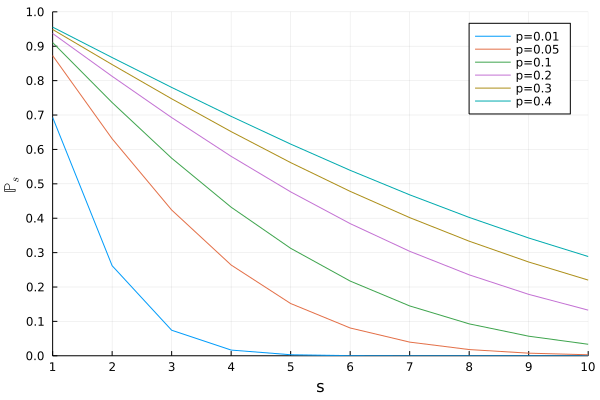
\includegraphics[width=.7\textwidth]{./figures/ps.png}
        \caption{Plot of $\mathbb{P}_s$ described in \autoref{obs:unfairness_fedsv}.}
        \label{fig:ps}
    \end{figure}
\end{observation}

The following numerical example corroborates this observation.

\begin{example}[Unfairness of FedSV] \label{ex:1}
    Consider the MNIST data set~\cite{lecun-mnisthandwrittendigit-2010}. Set the number of clients to be 10 with indices $I = \{0, \dots, 9\}$. Distribute the data for clients $0, \dots, 8$ in a non-IID fashion as described in \autoref{sec:7.6.1} and set client $9$'s data set to be the same as client $0$'s. We train a simple fully connected neural network model using \texttt{FedAvg} for 10 rounds and randomly select 3 clients in each round. We repeat this experiment 50 times. The empirical results show that the relative difference 
    \begin{equation} \label{eq:relative_difference}
            d_{0,9} = \frac{|s_0 - s_9|}{\max\{s_0, s_9\}}
    \end{equation}
    between the FedSVs of $s_0$ and $s_{9}$ is greater than 0.5 with probability 65\%. This simple result clearly shows that, although clients $0$ and $9$ have identical data, they receive dramatically different FEDSVs. FedSV violates the symmetry requirement of fairness.  
\end{example}


\section{Completed Federated Shapley Value} \label{sec:7.5}

In this section, we first design a utility matrix consisting of contributions of all subsets of clients over all rounds of training, and present the main theoretical result that the utility matrix is approximately low-rank when the local objectives are Lipschitz continuous and smooth. Then, based on a low-rank matrix completion formulation, we propose a new data evaluation method ComFedSV for federated learning. We also show that when the utility matrix can be well recovered, ComFedSV satisfies certain desirable fairness properties. Last, when the size of the utility matrix is too large, we develop a Monte-Carlo type sampling method to reduce the size of the corresponding matrix completion problem.

\subsection{Utility Matrix} \label{sec:7.5.1}
We design a matrix $\mathcal{U} \in \mathbb{R}^{T \times 2^N}$ that consists of all the possible utilities from any subsets of the clients over all the rounds. Each entry $(t, S)$ is defined as 
$\mathcal{U}_{t, S} = U_t(S)$. If we can compute matrix $\mathcal{U}$, we can obtain the fair Shapley value for every subset of clients in every round.

Since the central server randomly selects a subset $I_t \subseteq I$ of the clients in each round $t$, only a small number of the entries in matrix $\mathcal{U}$ are observed, that is, 
$\{\mathcal{U}_{t, S}: S \subseteq I_t, \enspace t \leq T\}$.
Based on this formulation, a natural question is whether we can get a good approximation for the missing values of the utility matrix $\mathcal{U}$. 

In order to complete a matrix with many missing entries, we have to explore the structure and the properties of the matrix. Our insight into the utility matrix is that, intuitively, it should be approximate low-rank. The rationale comes from at least two reasons. First, the clients with similar data should create similar utilities, which can lead to the similarity between columns of the utility matrix $\mathcal{U}$.  Moreover, if the user-specified loss function $\ell$ does not change dramatically over rounds, then the utilities by the same subset of clients should be similar between successive rounds, which can lead to the similarity between adjacent rows of the utility matrix $\mathcal{U}$.

Before we provide a concrete mathematical justification, let us employ some empirical examples to verify our insight. In the following example, we show that the utility matrix $\mathcal{U}$ is nearly low-rank in many circumstances, in the sense that only a few of its singular values are dominant and all the others are relatively negligible. 

\begin{example}[Low-rankness of Utility Matrix] \label{ex:2}
    We use three simple examples to show empirically that the utility matrix is approximately low-rank.  We train a logistic regression model, a fully connected neural network model, and a convolutional neural network model respectively for synthetic data, MNIST~\cite{lecun-mnisthandwrittendigit-2010}, and CIFAR10~\cite{Krizhevsky09learningmultiple} (see \autoref{sec:7.6} for a detailed description). On each data set, we have 10 clients, train the model for 100 rounds and randomly select 3 clients in each round. Thus, the utility matrix $\mathcal{U}$ has size $100\times 2^{10}$. Although we update the global model with the randomly selected clients in each round, in order to obtain the whole utility matrix, we do compute the updates of all clients in each round.
    
    The distribution of singular values is plotted in \autoref{fig:svds}. Clearly, the three different utility matrices are all nearly low-rank.

    \begin{figure}[t]
        \centering
        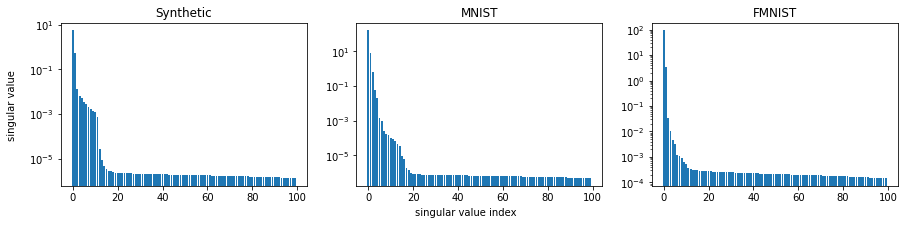
\includegraphics[width=\textwidth]{./figures/svds.png}
        \caption{Singular values of the utility matrices described in \autoref{ex:2}. In all cases, the matrices are nearly low-rank.}
        \label{fig:svds}
    \end{figure}

\end{example}

Next, we investigate theoretical guarantees to support our intuition. Before stating the result, we first revisit a formal definition of approximately low-rank~\cite{udell2019big}. 
\begin{definition}[$\epsilon$-rank]
    Let $X\in\mathbb{R}^{m\times n}$ be a matrix and $\epsilon>0$ a tolerance. The $\epsilon$-rank of $X$ is given by 
    \[\rank_{\epsilon}(X) = \min\{\rank(Z): Z\in\mathbb{R}^{m\times n}, \|Z - X\|_{\max} \leq \epsilon\},\]
    where $\|\cdot\|_{\max}$ is the absolute maximum matrix entry. Thus, $k = \rank_{\epsilon} (X)$ is the smallest integer for which $X$ can be approximated by a rank $k$ matrix, up to an accuracy of $\epsilon$.
\end{definition}

The following proposition formally characterizes the low-rankness of the utility matrix. We show that if all the losses are Lipschitz continuous and smooth, then the utility matrix is approximately low-rank. The definitions of convex, strongly-convex, Lipschitz, and smooth functions, as well as the proofs of the formal results in this section can be found in the appendices.

\begin{proposition}[Lipschitz continuous and smooth objective] \label{prop:lipschitz}
    Assume that the user specified loss function $\ell(w; D)$ is convex, $L_1$-Lipschitz continuous and $L_2$-smooth in $w$ for all $D \in \{D_c, D_1, D_2, \dots, D_N\}$, and the learning rates $\eta^t$ are non-increasing. 
    Then for any $\epsilon>0$, 
    \begin{equation} \label{eq:epsilon_rank_u}
        \rank_{\epsilon}(\mathcal{U}) \leq \left\lceil \frac{(2+\eta^1L_2) L_1 \sum_{t=1}^{T-1} \|w^{t} - w^{t+1}\| + (\eta^1 - \eta^T) L_1^2}{\epsilon} \right\rceil.
    \end{equation} 
\end{proposition}

\autoref{prop:lipschitz} suggests the question: Is there an upper bound on the right-hand side of~\eqref{eq:epsilon_rank_u}? The answer is affirmative, provided an additional assumption on the strong convexity of the loss functions. Li~\textit{et al.}~\cite{li2019convergence} proved that \texttt{FedAvg} converges with rate $\mathcal{O}(1 / T)$ when the local models are all smooth and strongly convex. Thus, we can bound the diameter of the set of global parameters $\{w^1, \dots, w^T\}$. The following result formalizes this observation. 

\begin{proposition}[Lipschitz, smooth and strongly convex objective] \label{prop:strongly_cvx}
    In addition to the setting in \autoref{prop:lipschitz}, we assume that the user specified loss function $\ell(w; D)$ is $\mu$-strongly convex w.r.t.\ $w$ for all $D \in \{D_c, D_1, D_2, \dots, D_N\}$, and the learning rates are defined by 
    \[\eta^t = \frac{2}{\mu(\gamma + t)} \enspace\text{with}\enspace \gamma = \max\left\{\frac{8\mu}{L_2}, 1\right\}.\]
    Then for any $\epsilon>0$, 
    \begin{align*}
        \rank_{\epsilon}(\mathcal{U}) &\leq \left\lceil \frac{2(2+\eta^1L_2) L_1 \log(T)}{\mu\epsilon} +  \frac{(\eta^1 - \eta^T)L_1^2}{\epsilon} \right\rceil
        \\&\in \mathcal{O}\left(\frac{\log(T)}{\epsilon}\right).
    \end{align*}
\end{proposition}
This promising result shows that the $\epsilon$-rank of the utility matrix $\mathcal{U}$ is of order $\log(T)$ and is independent of the number of clients. The parameter $\epsilon$ controls the tradeoff between rank and approximation accuracy.

The sufficient conditions in \autoref{prop:lipschitz} and~\autoref{prop:strongly_cvx} cover a class of Lipschitz continuous, smooth and strongly convex functions, which appear in a wide range of machine learning and optimization problems, including regularized linear regression and logistic regression. This class of functions have many good properties in the sense that neither the function itself nor its gradient has sharp changes. Geometrically, for a set of clients, these two properties can imply the similarity between their contributions over successive rounds, which leads to the low-rank property as stated in \autoref{prop:lipschitz}and~\autoref{prop:strongly_cvx}. For more general loss functions, i.e., neural networks, although the sufficient conditions are not met, we empirically show that the utility matrix is still approximately low rank (\autoref{ex:2}).

\subsection{Everyone Being Heard Assumption}

\autoref{prop:lipschitz} and~\autoref{prop:strongly_cvx}, together with our empirical observation, imply that the utility matrix $\mathcal{U}$ is approximately low-rank when the loss function enjoys certain standard properties. The low-rank structure of the utility matrix suggests that we can approximate the missing entries of $\mathcal{U}$ by solving a low-rank matrix completion problem.

Before describing the low-rank matrix completion problem, we need to introduce a natural assumption. Note that if one client never reports its local model to the server, 
the central server does not get a chance to observe the possible contribution by the client. Consequently, the contribution of the client cannot be estimated. To tackle this issue, we assume that every client is willing to participate in the federated learning in each round.  Therefore, no matter a client is selected by the server in a round, the potential value of the client should be recognized properly.  Formally, we have the following assumption.

\begin{assumption}[Everyone Being Heard] \label{ass:main}
The central server selects all clients for update in at least one round, that is, there exists $k>0$, $I_k = I$.  Without loss of generality, in the rest of the paper, we assume $I_1=I$. Our discussion can be easily generalized to any $I_k=I$.
\end{assumption}

Note that \autoref{ass:main} does not come with high costs. As explained in \autoref{sec:7.1}, the central server selects a subset of clients in each round only to reduce communication cost, and the communication cost for doing one round of all clients is equivalent to doing $\left \lceil{N / m}\right \rceil $ rounds of additional training, where $m = |I_t|$ for all $t$. 

\subsection{Approximately Low-Rank Matrix Completion} \label{sec:7.5.2}

We propose the following factorization-based low-rank matrix completion problem to complete the utility matrix $\mathcal{U}$: 
\begin{equation}
\label{prob:matrix_completion}
\minimize{\substack{W \in \mathbb{R}^{T \times r}\\ H \in \mathbb{R}^{2^N \times r}}} \enspace \sum_{t=1}^T\sum_{S\subseteq I_t} (\mathcal{U}_{t,S} - w_t^Th_{S})^2 + 
\lambda(\|W\|_F^2 + \|H\|_F^2),
\end{equation}
where $r$ is a user specified rank parameter, $\lambda$ is a positive regularization parameter, $\|\cdot\|_F$ is the Frobenious norm, and $w_t$ and $h_S$, respectively, are the $t$-th and the $S$-th row vectors of the matrices $W$ and $H$. Because the matrix completion problem~\eqref{prob:matrix_completion} is solved after the whole training process, we can determine the rank parameter $r$ via \autoref{prop:lipschitz} and~\autoref{prop:strongly_cvx}. We show the impact of rank parameter $r$ on the performance of the low-rank matrix completion problem~\eqref{prob:matrix_completion} via a numerical example.

\begin{example}[Impact of Rank Parameter] \label{ex:3}
    We conduct a numerical experiment to show the impact of the rank parameter $r$ on the matrix completion problem~\eqref{prob:matrix_completion}. We train a simple multilayer perceptron neural network for the MNIST data set. We have 10 clients, train the model for 100 rounds and randomly select 3 clients in each round. Note that although we update the global model with the selected clients, in order to get the whole utility matrix, we compute the updates of all clients in each round. We define the relative difference between $\mathcal{U}$ and $WH^T$ as 
    $\frac{\|\mathcal{U} - WH^T\|_{Fro}}{\|\mathcal{U}\|_{Fro}}$.
    We try different rank parameters $r \in \{1, \dots, 10\}$ and report the relative difference in \autoref{fig:rank}. The curve shows that a small rank parameter may not be enough for recovering the information in the utility matrix $\mathcal{U}$ and a large rank parameter may bring some overfitting problem.  
    
    \begin{figure}[t]
        \centering
        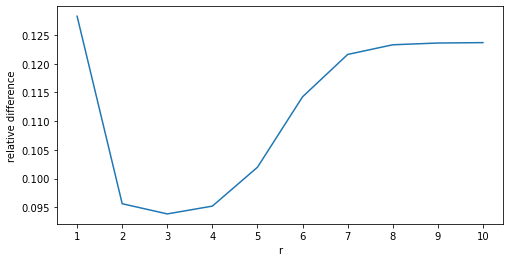
\includegraphics[width=.7\textwidth]{./figures/rank_impact.png}
        \caption{Impact of rank parameter described in \autoref{ex:3}.}
        \label{fig:rank}
    \end{figure}
    
\end{example}

Interestingly, the low-rank matrix completion model~\eqref{prob:matrix_completion} was first used in completing the information for recommender systems~\cite{koren2009matrix}. Its effectiveness has been extensively studied both theoretically and empirically~\cite{keshavan2012efficient, sun2016guaranteed}.  Therefore, we can simply adopt the well established matrix completion methods~\cite{yu2014parallel, chin2016libmf} and focus on how to derive fair contribution evaluation metric based on a completed utility matrix.
    
\subsection{Completed Federated Shapley Value} \label{sec:5.3}

\begin{figure}[t]
    \centering
    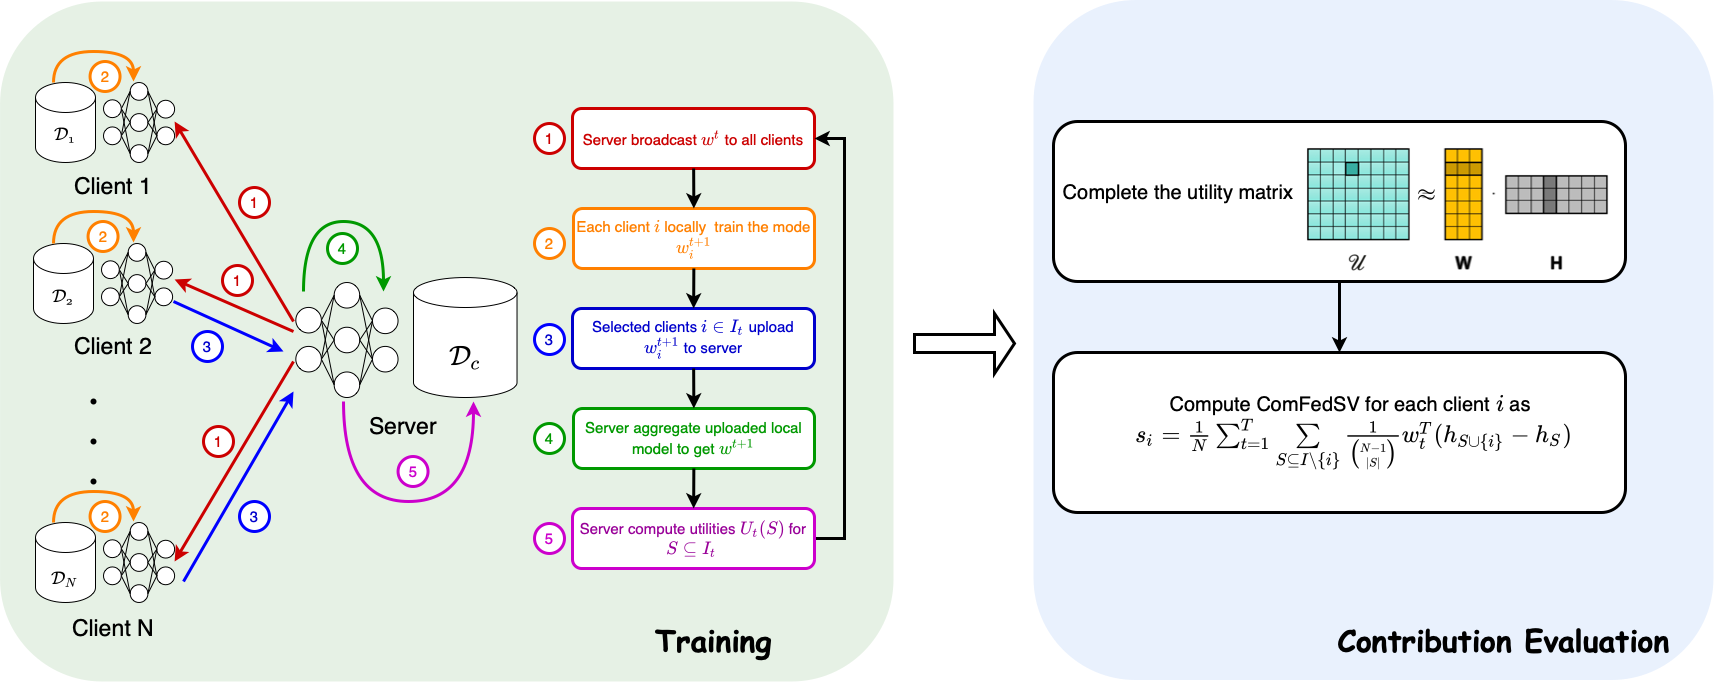
\includegraphics[width=\textwidth]{./figures/DataValuation.drawio.png}
    \caption{Pipeline of data valuation in horizontal federated learning.}
    \label{fig:pipeline}
\end{figure}

Now, we are ready to give the formal definition of ComFedSV. 
\begin{definition}[Completed Federated Shapley Value (ComFedSV)] \label{def:complete_sv}
    Let $W$ and  $H$ be the optimal solutions to the approximately low-rank matrix completion problem~\eqref{prob:matrix_completion}. Then, the ComFedSV for each client $i \in I$ is defined as 
    \begin{equation} \label{eq:complete_sv}
        s_i = \frac{1}{N} \sum_{t=1}^T\sum\limits_{S \subseteq I \setminus\{i\}} \frac{1}{\binom{N-1}{|S|}} w_t^T(h_{S\cup\{i\}} - h_S),
    \end{equation}
    where $w_t$ and $h_S$, respectively, are the $t$-th and the $S$-th row vectors of the matrices $W$ and $H$.
\end{definition}
The whole pipeline is shown in \autoref{fig:pipeline}. The next result shows that if we can approximately recover the utility matrix, then ComFedSV is guaranteed to be approximate Shapley-fair according to \autoref{def:fairness}. We first give a formal definition of the approximate recovery of the utility matrix. 

\begin{definition} \label{def:completeness}
    Let $W$ and  $H$ be the optimal solutions to the approximately low-rank matrix completion problem~\eqref{prob:matrix_completion}, and $s$ be the ComFedSV (\autoref{def:complete_sv}). We say that $s$ is \textbf{$\delta$-completed} for some $\delta>0$, if we can complete the utility matrix with tolerance $\delta$, that is,
    $\|\mathcal{U} - W H^T\|_1 \leq \delta$, where
    $\|\cdot\|_1$ is the maximum absolute column sum, i.e., $\|X\|_1 = \max_j \sum_i |X_{i,j}|$. 
\end{definition}

We now state our theoretical guarantee on the fairness of the ComFedSV. 

\begin{theorem}[Fairness Guarantee] \label{prop:fair}
    Let $U: 2^I \to \mathbb{R}$ be the utility function for the whole training process in federated learning: 
    \[U(S) = \sum_{t=1}^T U_t(S) \enspace \forall S \subseteq I.\]
    Let $s$ be the ComFedSV computed with respect to $U$.  Then, $s$ is $(\frac{4\delta}{N})$-Shapley-fair if
    \begin{enumerate}
        \item  $s$ is $\delta$-completed for some $\delta > 0$; and 
        \item if $U = U_1 + U_2$ and $s_1, s_2$ are the ComFedSVs computed with respect to utility functions $U_1$ and $U_2$, respectively, then $s_i$ $(i \in \{1,2\})$ is $\delta_i$-completed such that $\delta_1 + \delta_2 \leq \delta$. 
    \end{enumerate}
\end{theorem}

In particular, as long as the utility matrix is perfectly recovered, i.e., $\mathcal{U} = WH^T$, \autoref{prop:fair} guarantees that clients with identical local data obtain the same evaluation.

There are different kinds of fairness in machine learning and federated learning~\cite{zemel2013learning,donini2018empirical,li2019fair,lyu2020collaborative,chu2021fedfair}. In this work, we focus on the fairness in data valuation (\autoref{prop:fair}). Moreover, our proposed metric is adaptable to different training algorithms for federated learning. When there are training algorithms that can achieve some other requirements on fairness besides the ones described in the paper, it is possible to combine those training algorithms with our valuation metric. For example, Chu et al.~\cite{chu2021fedfair} proposed an algorithm that can guarantee the fairness for protected groups. Our valuation metric ComFedSV can be easily adapted to their algorithm since we still have access to the uploaded local models in each iteration.

\subsection{Estimating ComFedSV} \label{sec:7.5.4}

\begin{algorithm}[t]
    \DontPrintSemicolon
    \caption{Estimating the ComFedSV} \label{alg:main}
    \KwIn{$I$: set of clients\\
        \hspace{9mm} $T$: number of rounds\\
        \hspace{9mm} $K$: number of selected clients per round\\
        \hspace{9mm} $M$: number of Monte Carlo samples
        }
    Initialize utility matrix $\mathcal{U} \in \mathbb{R}^{T\times MN}$ with all $0$'s\;
    Initialize the global model parameter $w^0 \in \mathbb{R}^n$\;
    Uniformly sample $M$ permutations of $I$: $\pi_1, \dots, \pi_M$\;
     \For{t = 0, \dots, T}{
        
        \For{$i$ in $I$}{
            Synchronize the global model $w_i^t = w^t$\;
            Update the local model as in~\eqref{eq:local_step}\;
        }
        
        \eIf{t = 0}{
            $I_t = I$; see \autoref{ass:main}\;
        }{
            Uniformly sample $I_t \subset I$ with $|I_t| = K$\;
        }
        
        Update the global model as in~\eqref{eq:global_step}\;
        
        \For{m = 1, \dots, M}{
            \For{$i$ in $I$}{
                \If{$\pi_m(i) \subseteq I_t$}{
                    $\mathcal{U}_{t,\pi_m(i)} = u_t(\pi_m(i))$;
                }
            }
        }
     }
     Solve problem~\eqref{prob:matrix_completion_reduced} to get $W$ and $H$\;
     \For{$i$ in $I$}{
        Compute the completed Shapley value $s_i$ as in~\eqref{eq:complete_ev_approx}\;
     }
     \Return{ $\{s_i: i \in I\}$ }
\end{algorithm}

The utility matrix $\mathcal{U}$ has size $T \times 2^N$, which is exponential in the number of clients. As the number of clients increases, solving the matrix completion problem~\eqref{prob:matrix_completion} cannot scale up. The similar situation appears in the computation of the Shapley value, where the computational complexity is also exponential in the number of clients. Can we estimate the Shapley values in our model?

How to efficiently estimatie the Shapley value has been studied extensively~\cite{ghorbani2019data,jia2019towards}. Here we describe the well known Monte-Carlo sampling method~\cite{metropolis1949monte, ghorbani2019data}. We can rewrite the definition of ComFedSV~\eqref{eq:complete_sv} into an equivalent formulation using expectation:
\begin{equation} \label{eq:complete_ev_expectation}
    s_i = \mathop{\mathbb{E}}_{\pi \sim \Pi(I)} \sum_{t=1}^T w_t^T\left(h_{ \pi(i) \cup \{i\}}  - h_{ \pi(i) }\right),
\end{equation}
where $\Pi(I)$ is the uniform distribution over all $N!$ permutations of the set of clients $I$ and $\pi(i)$ is the set of clients preceding client $i$ in permutation $\pi$. With this formulation, we can use the Monte-Carlo method to get an approximation of ComFedSV. More precisely, we can randomly sample $M$ permutations $\pi_1, \dots, \pi_M$ and get an approximation to ComFedSV $s_i$ by 
\begin{equation} \label{eq:complete_ev_approx}
    \hat s_i = \frac{1}{M}\sum_{m=1}^M \sum_{t=1}^T w_t^T\left(h_{ \pi_m(i) \cup \{i\}}  - h_{ \pi_m(i) }\right).
\end{equation}

From~\eqref{eq:complete_ev_approx}, we notice that we only need access to part of the utility matrix $\mathcal{U}$, namely 
\[ \{\mathcal{U}_{t, S}: t \in [1, \dots, T], S = \pi_m(i), m \in [1,\dots,M], i \in I\}, \]
which suggests that we can reduce the size of the matrix completion problem~\eqref{prob:matrix_completion}. Formally, we can solve the following reduced matrix completion problem:
\begin{equation}
\label{prob:matrix_completion_reduced}
\minimize{\substack{W \in \mathbb{R}^{T \times r}\\ H \in \mathbb{R}^{MN \times r}}}\enspace \sum_{t=1}^T\sum_{ \substack{m \in [1,\dots, M] \\ i \in I \\ \pi_m(i) \subseteq I_t  } } (\mathcal{U}_{t,\pi_m(i)} - w_t^Th_{\pi_m(i)})^2 + \lambda(\|W\|_F^2 + \|H\|_F^2).
\end{equation}

We summarize the whole process in \autoref{alg:main}. It was shown by \cite{maleki2013bounding} that, for bounded utility functions, the Monte-Carlo method requires $M = \mathcal{O}(N\log N)$ samples to achieve a good approximation.  The estimation is unbiased. As a consequence, both the space and time complexities for \autoref{alg:main} are $\mathcal{O}(TN^2\log(N))$. 

\section{Experiments} \label{sec:7.6}
This section reports a series of experiments that examine how well ComFedSV can capture contributions from clients/data owners in federated learning. Our code is publicly available at the \emph{Huawei AI Gallery}\footnote{\url{https://developer.huaweicloud.com/develop/aigallery/notebook/detail?id=08da32bb-9b85-4ddb-ae6c-94a3f5102133}}.

\subsection{Experiment Setting} \label{sec:7.6.1}

\subsubsection{Data Sets} 
We perform experiments on both real and synthetic data. For synthetic data, we follow the setup as in~\cite{li2018federated}. For real data, we choose the widely used benchmark data sets MNIST~\cite{lecun-mnisthandwrittendigit-2010}, Fashion MNIST~\cite{xiao2017fashion}, and CIFAR10~\cite{krizhevsky2009learning}.  

In reality, data sets from different data owners may have different distributions. To model this circumstance, for each data set, we consider two different ways for distributing the data: IID and non-IID. For synthetic data, according to \cite{li2018federated}, the data set has two parameters $\alpha$ and $\beta$, where $\alpha$ controls how much local models differ from each other and $\beta$ controls how much local data sets differ from each other. We choose $\alpha=0, \beta=0$ for IID and $\alpha=1, \beta=1$ for non-IID. For real data sets MNIST, Fashion MNIST, and CIFAR10, we randomly distributed the data to all clients for IID, and each client gets samples of only two classes for non-IID, which is the same setting as in the original \texttt{FedAvg} paper~\cite{mcmahan2017communication}.


\subsubsection{Model} 
For synthetic data, we train a logistic regression model. We run 100 rounds of training and can achieve up to $99\%$ and $95\%$ classification accuracies on the test set in the cases of IID and non-IID, respectively. For MNIST, we train a fully connected neural network. We run 100 rounds of training and can achieve up to $98\%$ and $92\%$ classification accuracies on the test set in the IID and non-IID settings, respectively. For Fashion MNIST, we train a simple convolutional neural network. We run 100 rounds of training and can achieve up to $98\%$ and $90\%$ classification accuracies on the test set in the cases of IID and non-IID, respectively. For CIFAR10, we train a VGG16 model~\cite{simonyan2014very}, which is a more complex convolutional neural network. We run 100 rounds of training and can achieve up to $91\%$ and $83\%$ classification accuracies on the test set in the cases of IID and non-IID, respectively, where we use a pre-trained model for non-IID.  We use different models to test the generality of our method. 

\subsubsection{Solver for Matrix Completion} 
We use the open source package \texttt{LIBPMF}\footnote{\url{https://github.com/cjlin1/libmf}}~\cite{chin2016libmf} to solve the matrix completion problem~\eqref{prob:matrix_completion_reduced}.

\subsubsection{Compared metrics} 
We compare the performance of ComFedSV with FedSV and the ground-truth, where the ground-truth is ComFedSV computed from the full utility matrix. Note that for the ground-truth, although we compute the updates of all clients in each round to obtain the whole utility matrix, we only update the global model with the updates by the randomly selected clients in each round, so that the global models will be the same for all three metrics.

\subsection{Fairness} \label{sec:7.6.2}

\begin{figure}[t]
    \centering
    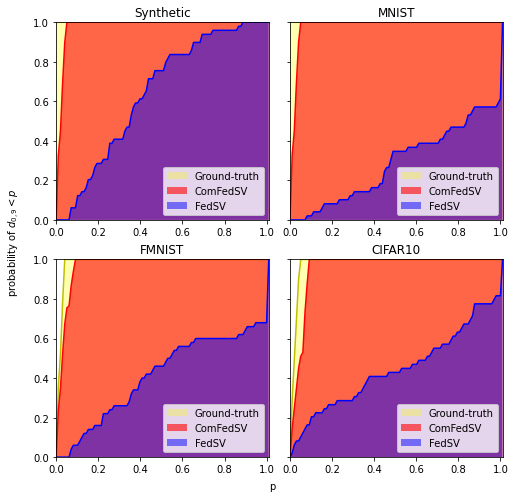
\includegraphics[width=.8\textwidth]{./figures/equal_data.png}
    \caption{Fairness: the empirical cumulative distribution of the relative difference between the evaluation metrics (FedSV and ComFedSV) of clients 0 and 9, which are set to have the identical local data sets.}
    \label{fig:fairness}
\end{figure}

In this experiment, we extend the results shown in \autoref{ex:1} and investigate whether ComFedSV improves fairness by checking if clients with similar data sets receive similar ComFedSVs. Limited by space, we only discuss the non-IID setting here.

\autoref{fig:fairness} shows the empirical cumulative distribution of the relative difference $d_{0,9}$ between clients 0 and 9, where we use two metrics: FedSV and ComFedSV. The relative difference is defined by \eqref{eq:relative_difference}, and takes values between $0$ and $1$. The vertical axis represents the probability $\mathbb{P}(d_{0,9} \leq t)$. Clearly, ComFedSV outperforms FedSV in fairness. On all data sets, Synthetic, MNIST, FMNIST, and CIFAR10, the probability $\mathbb{P}(d_{0,9}^{ComFedSV} < t)$ is always greater than or equal to $\mathbb{P}(d_{0,9}^{FedSV} < t)$ for all possible value of $t$. In other words, in most trials, clients with same local data receive more similar evaluations in ComFedSV, but receive quite different evaluations in FedSV.

\subsection{Data Quality Detection} \label{sec:7.6.3}

Wang~\textit{et al.}~\cite{wang2020principled} showed that FedSV can be used to detect data quality.  To make a fair comparison, we conduct a similar experiment to compare the data quality detection capability of ComFedSV and FedSV.

Typically, two types of noise, data noise and label noise, is considered. The literature usually treats the percentage of noisy data points and noisy labels as the measures for the quality of data sets~\cite{liebchen2008data, karimi2020deep}. 
We start from the IID partitioning of the data to clients and then add different amounts of noise to different clients. After the noise is added, the data used in federated learning is not IID anymore.

\subsubsection{Noisy Data Detection}

\begin{figure}[t]
    \centering
    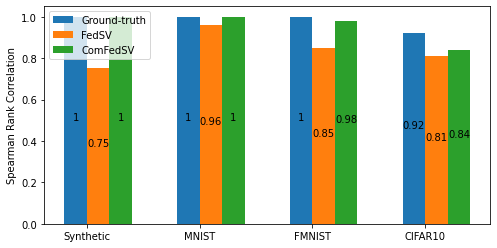
\includegraphics[width=.7\linewidth]{./figures/data_noise_detection.png}
    \caption{Noisy data detection: the Spearman’s  rank  correlation between the true ranking and the rankings produced by the three metrics (ground-truth, FedSV and ComFedSV).}
    \label{fig:noisy_data_detection}
\end{figure}

We set 10 clients: $I = \{0, 1, \dots, 9\}$, run federated learning for 10 rounds and randomly select 3 clients to report in each round. For each client $i \in I$, we artificially add Gaussian noise to $5\times i\%$ of their data. Under this setting, the descending order of clients in the amount of noise added is $9, 8, \dots, 0$.  We compute the ground-truth, FedSV, and ComFedSV for all clients and compare the rankings produced by those three metrics. We use Spearman's rank correlation~\cite{zar1972significance,zar2005spearman} to measure the similarity between the true ranking $9, 8, \dots, 0$ and the rankings produced by the three metrics. The result is shown in \autoref{fig:noisy_data_detection}. ComFedSV outperforms FedSV and almost matches the ground-truth on all four data sets. This experiment clearly shows that ComFedSV has a strong capability in detect data quality for machine learning models, even better than that of FedSV.

\subsubsection{Noisy Label Detection}

\begin{figure}[t]
    \centering
    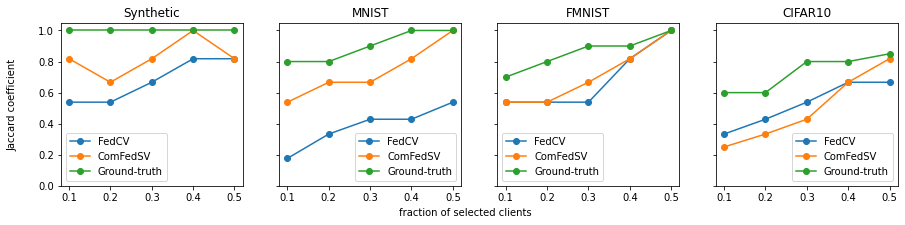
\includegraphics[width=\textwidth]{./figures/label_noise_detection.png}
    \caption{Noisy label detection: the Jaccard coefficient between the set of 10 clients with noisy labels and the set of 10 clients with the lowest evaluations (FedSV and ComFedSV).}
    \label{fig:noisy_label_detection}
\end{figure}

We set 100 clients such that 10 of them each has 30\% noisy labels, where noise is introduced by random flipping. For each data set, we conduct federated learning for 100 rounds and randomly select $m\%$ clients to report in each round with $m \in \{10, 20 , \dots, 50\}$. We compare FedSV and ComFedSV by the Jaccard coefficient~\cite{jaccard1912distribution} between the set of  clients with the noisy labels and the set of 10 clients with the lowest evaluations. The result is shown in \autoref{fig:noisy_label_detection}. ComFedSV outperforms FedSV in most cases. Both methods perform better as more clients are selected to report in each round.

\subsection{Time Complexity} \label{sec:time}

\begin{figure}[t]
    \centering
    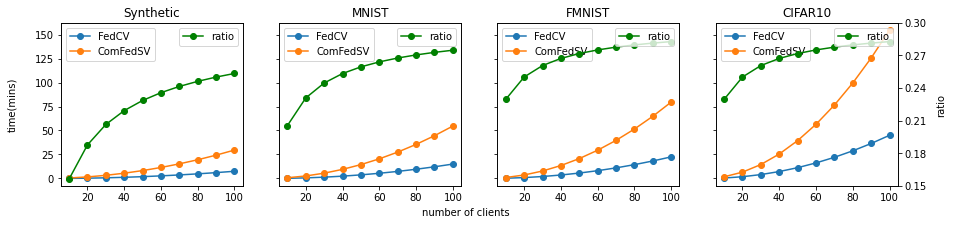
\includegraphics[width=\textwidth]{./figures/time_performance.png}
    \caption{Computing time comparison. The orange and blue curves correspond to the computing time for FedSV and ComFedSV respectively (left y-axis). The green curve the the ratio between the computing time for FedSV and ComFedSV (right y-axis).}
    \label{fig:time_performance}
\end{figure}

In this experiment, we compare the time required for computing ComFedSV and FedSV. Although the time complexity for \autoref{alg:main} is $\mathcal{O}(TN^2\log(N))$, the main cost is evaluating the roundly utility function $u_t$, which requires computing the test loss of the model. It is easy to see that in \autoref{alg:main}, the number of calls to $u_t$ is in $\mathcal{O}(TNKlog(N))$, where $K$ is the number of selected clients per round. As a comparison, computing FedSV with Monte-Carlo requires $\mathcal{O}(TK^2log(K))$ calls. This suggests that the ratio between the number of calls for FedSV and ComFedSV is $\mathcal{O}(\frac{K}{N})$, which equals to the random participation rate.

We set the number of clients to $10, 20, \dots, 100$ and randomly select $30\%$ of clients to report in each round. The results are shown in \autoref{fig:time_performance}, where we plot the computing time for FedSV and ComFedSV (left y-axis), as well as their ratio (right y-axis). As we can see from the plots, the ratio between the computing time for FedSV and ComFedSV is approaching a stable constant close to the participation rate as the number clients increases, which agrees with our complexity analysis.

\section{Future Directions}
In this paper, we tackle the challenging problem of data valuation in horizontal federated learning. We point out the possible unfairness in the existing data valuation method. Then, we propose a new measure ComFedSV, which is not only fair with theoretical guarantee, and also can be evaluated efficiently. We verify the fairness of our measure both theoretically and experimentally. 

Our study advances the frontier in this emerging important direction. There are also many interesting future directions.  For example, it is interesting to extend our methodology to vertical federated learning. As another example, under the framework of federated learning, there may exist some other properties needed for fairness in federated learning in addition to those in the Shapley fairness.

\section{Proofs}

\subsection{Derivation of \autoref{obs:unfairness_fedsv}}
In this section, we show the derivation of the probabilistic bound in \autoref{obs:unfairness_fedsv}. For any $t \in \{1, \dots, T\}$, we define $\alpha_t := s_{t,i} - s_{t,j}$. Then $|s_i - s_j| = |\sum_{t=1}^T \alpha_t|$. By the assumption in \autoref{obs:unfairness_fedsv} and definition of FedSV (\autoref{def:federated_sv}), it follows that $\alpha_t$ can be expressed as 
\[\alpha_t = 
\begin{cases} 
      \delta_t & i \in I_t ~\text{and}~ j \notin I_t \\
      0 & i,j \in I_t ~\text{or}~ i,j \notin I_t\\
      -\delta_t & i \notin I_t ~\text{and}~ j \in I_t. 
\end{cases}
\]
We define some auxiliary variables $\beta_t$ for $t \in \{1, \dots, T\}$ as 
\[\beta_t = 
\begin{cases} 
      \delta & i \in I_t ~\text{and}~ j \notin I_t \\
      0 & i,j \in I_t ~\text{or}~ i,j \notin I_t\\
      -\delta & i \notin I_t ~\text{and}~ j \in I_t. 
\end{cases}
\]
Then we derive the probabilistic bound for $\sum_{t=1}^T \beta_t$. For any $s \in \{1, \dots, T\}$,
\begin{align*}
    &\mathbb{P}\left(\sum_{t=1}^T \beta_t \geq s\delta\right) 
    \\=&\sum_{a = s}^T \mathbb{P}\left(\sum_{t=1}^T \beta_t = a\delta\right)
    \\=&\sum_{a = s}^T \sum_{b=0}^{\floor{\frac{n-a}{2}}} \binom{T}{b,, T - a - 2b, b+a} p^{2b + a} (1-p)^{T - 2b - a},
\end{align*}
where
\[p = \mathbb{P}(i \in I_t ~\text{and}~ j \notin I_t) = \frac{m(n-m)}{n(n-1)}.\]
Finally, we derive the probability bound of $|s_i - s_j| \geq s\delta$ for any $s \in \{1, \dots, T\}$:
\begin{align*}
    &\mathbb{P}(|s_i - s_j| \geq s\delta) 
    \\=&\mathbb{P}\left(|\sum_{t=1}^T \alpha_t| \geq s\delta\right)
    \\=&2\mathbb{P}\left(\sum_{t=1}^T \alpha_t \geq s\delta\right)
    \\\geq&2\mathbb{P}\left(\sum_{t=1}^T \alpha_t \geq s\delta ~\bigg\vert~ \sum_{t=1}^T \beta_t \geq s\delta \right) \mathbb{P}\left(\sum_{t=1}^T \beta_t \geq s\delta\right)
    \\=& \sum_{a = s}^T \sum_{b=0}^{\floor{\frac{n-a}{2}}} \binom{T}{b,, T - a - 2b, b+a} p^{2b + a} (1-p)^{T - 2b - a},
\end{align*}
where the last equality follows from the fact 
\[\mathbb{P}\left(\sum_{t=1}^T \alpha_t \geq s\delta ~\bigg\vert~ \sum_{t=1}^T \beta_t \geq s\delta \right) = \frac{1}{2}.\]


\subsection{Proof for \autoref{prop:lipschitz}}
In this section, we provide the proof for \autoref{prop:lipschitz}. 
\begin{proof}
    First, we bound the difference between utilities by the same subset of clients over successive rounds. Specifically, for any $t\in\{1,\dots,T-1\}$ and $S \subseteq I$, we have 
    \begin{align*}
        &|U_{t}(S) - U_{t+1}(S)|\\
        = &|\ell(w^{t}; D_c) - \ell(w_S^{t+1}; D_c) - \ell(w^{t+1}; D_c) + \ell(w_S^{t+2}; D_c)|
        \\\leq &|\ell(w^{t}; D_c) - \ell(w^{t+1}; D_c)| + |\ell(w_S^{t+1}; D_c) - \ell(w_S^{t+2}; D_c)|
        \\\leq &L_1\|w^{t} - w^{t+1}\| + L_1\|w_S^{t+1} - w_S^{t+2}\|
        \\= &L_1\|w^{t} - w^{t+1}\| + L_1\bigg\|w^{t} - \frac{\eta^t}{|S|}\sum_{i\in S} \nabla F_i(w^{t})
        \\&  - w^{t+1} + \frac{\eta^{t+1}}{|S|}\sum_{i\in S} \nabla F_i(w^{t+1}) \bigg\|
        \\\leq &2L_1\|w^{t} - w^{t+1}\| + \frac{L_1\eta^{t+1}}{|S|}\sum_{i\in S}\left\|\nabla F_i(w^{t}) - \nabla F_i(w^{t+1})\right\| 
        \\&+ \frac{L_1(\eta^{t} - \eta^{t+1})}{|S|}\sum_{i\in S}\left\|\nabla F_i(w^{t})\right\|
        \\\leq &(2+\eta^1L_2) L_1\|w^{t} - w^{t+1}\| + (\eta^{t} - \eta^{t+1})L_1^2.
    \end{align*}
    Then we can get an upper bound on the sum of all maximum entry-wise norm between successive rows of the utility matrix, namely
    \begin{align*}
        &~\sum_{t=1}^{T-1} \left\|\mathcal{U}[t,:] - \mathcal{U}[t+1,:]\right\|_{\max} \\
        \leq &~\sum_{t=1}^{T-1}\left[ (2+\eta^1L_2) L_1\|w^{t} - w^{t+1}\| + (\eta^{t} - \eta^{t+1})L_1^2 \right]
        \\= &~(2+\eta^1L_2) L_1 \sum_{t=1}^{T-1} \|w^{t} - w^{t+1}\| + (\eta^1 - \eta^T)L_1^2.
    \end{align*}
    Therefore, it follows that 
    \begin{equation*}
        \rank_{\epsilon}(\mathcal{U}) \leq \left\lceil \frac{(2+\eta^1L_2) L_1 \sum_{t=1}^{T-1} \|w^{t} - w^{t+1}\| + (\eta^1 - \eta^T)L_1^2}{\epsilon} \right\rceil.
    \end{equation*}
\end{proof}

\subsection{Proof for \autoref{prop:strongly_cvx}}
In this section, we provide the proof for \autoref{prop:strongly_cvx}. 
\begin{proof}
 By \cite[Theorem~1]{li2019convergence}, we know that the based on the setting in \autoref{prop:strongly_cvx}, the \texttt{FedAvg} can have sublinear convergence rate. Now we will give an upper bound on the length of path of the global parameters $w^t$: 
 \[\sum_{t=1}^{T-1} \|w^{t+1} - w^t\| = \sum_{t=1}^{T-1} \eta^t \leq \sum_{t=1}^{T-1} \frac{2}{\mu t} \leq \frac{2}{\mu} \log(T).\]
 Now combine with the result in \autoref{prop:lipschitz}, we have the following upper bound on the $\epsilon$-rank of the utility matrix $\mathcal{U}$:
 \[\rank_{\epsilon}(\mathcal{U}) \leq \left\lceil \frac{2(2+\eta^1L_2) L_1 \log(T)}{\mu\epsilon} +  \frac{(\eta^1 - \eta^T)L_1^2}{\epsilon} \right\rceil.\]
\end{proof}

\subsection{Proof for \autoref{prop:fair}}
In this section, we provide the proof for \autoref{prop:fair}. 
\begin{proof}
We denote the ComFedSV computed from the true utility matrix $\mathcal{U}$ as 
\begin{equation}
    \hat s_i = \frac{1}{N} \sum_{t=1}^T\sum\limits_{S \subseteq I \setminus\{i\}} \frac{1}{\binom{N-1}{|S|}} \left[ U_t(S \cup\{i\}) - U_t(S)\right].
\end{equation}

First, we show that $\hat s_i$'s strictly satisfy the \textbf{Symmetry}, \textbf{Zero element} and \textbf{Additivity} properties.
\begin{itemize}
    \item \textbf{Symmetry.} For any two clients $i,j \in I$. Suppose that for any subset of clients $S \subseteq I \setminus \{i,j\}$, $U(S \cup \{i\}) = U(S \cup \{j\})$. Then, 
    \begin{align*}
        \hat s_i = &~ \frac{1}{N} \sum_{t=1}^T\sum\limits_{S \subseteq I \setminus\{i\}} \frac{1}{\binom{N-1}{|S|}} \left[ U_t(S \cup\{i\}) - U_t(S)\right] \\
        = &~\frac{1}{N}\sum\limits_{S \subseteq I \setminus\{i\}} \frac{1}{\binom{N-1}{|S|}} \left[\sum_{t=1}^T U_t(S \cup\{i\}) - \sum_{t=1}^T U_t(S)\right]\\
        = &~\frac{1}{N}\sum\limits_{S \subseteq I \setminus\{i,j\}} \biggl\{\frac{1}{\binom{N-1}{|S|}} \left[\sum_{t=1}^T U_t(S \cup\{i\}) - \sum_{t=1}^T U_t(S)\right]  
        \\& + \frac{1}{\binom{N-1}{|S|+1}} \left[\sum_{t=1}^T U_t(S \cup\{j\}\cup\{i\}) - \sum_{t=1}^T U_t(S\cup\{j\})\right]\biggr\}\\
        = &~ \frac{1}{N}\sum\limits_{S \subseteq I \setminus\{i,j\}} \biggl\{\frac{1}{\binom{N-1}{|S|}} \left[U(S \cup\{i\}) - U(S)\right]  
        \\& + \frac{1}{\binom{N-1}{|S|+1}} \left[U(S \cup\{j\}\cup\{i\}) -  U(S\cup\{j\})\right]\biggr\}\\
        = &~ \frac{1}{N}\sum\limits_{S \subseteq I \setminus\{i,j\}} \biggl\{\frac{1}{\binom{N-1}{|S|}} \left[U(S \cup\{j\}) - U(S)\right]  
        \\& + \frac{1}{\binom{N-1}{|S|+1}} \left[U(S \cup\{j\}\cup\{i\}) -  U(S\cup\{i\})\right]\biggr\}\\
        = &~\hat s_j.
    \end{align*}
    \item \textbf{Zero element.} For any client $i \in I$. Suppose that for any subset of clients $S \subseteq I \setminus \{i\}$, $U(S \cup \{i\}) = U(S)$. Then, 
    \begin{align*}
        \hat s_i &= \frac{1}{N} \sum_{t=1}^T\sum\limits_{S \subseteq I \setminus\{i\}} \frac{1}{\binom{N-1}{|S|}} \left[ U_t(S \cup\{i\}) - U_t(S)\right] \\
        &= \frac{1}{N}\sum\limits_{S \subseteq I \setminus\{i\}} \frac{1}{\binom{N-1}{|S|}} \left[\sum_{t=1}^T U_t(S \cup\{i\}) - \sum_{t=1}^T U_t(S)\right]\\
        &= \frac{1}{N}\sum\limits_{S \subseteq I \setminus\{i\}} \frac{1}{\binom{N-1}{|S|}} \left[ U(S \cup\{i\}) - U(S)\right] = 0.
    \end{align*}
    \item \textbf{Additivity.} If the utility function $U$ can be expressed as the sum of separate utility functions, namely $U = U_1 + U_2$ for some $U_1, U_2 : 2^I \to \mathbb{R}$, then for any client $i \in I$, we have
    \begin{align*}
        \hat s_i 
        = & \frac{1}{N}\sum\limits_{S \subseteq I \setminus\{i\}} \frac{1}{\binom{N-1}{|S|}} \left[ U(S \cup\{i\}) - U(S)\right] 
        \\= &\frac{1}{N}\sum\limits_{S \subseteq I \setminus\{i\}} \frac{1}{\binom{N-1}{|S|}} \bigg[ U_1(S \cup\{i\}) + U_2(S \cup\{i\}) 
        \\&- U_1(S) - U_2(S)\bigg] 
        \\=& \hat s_{1,i} + \hat s_{2, i},
    \end{align*}
    where $\hat s_{1,i}$ and $\hat s_{2, i}$ are respectively the ComFedSVs computed from the true utility matrices $\mathcal{U}_1$ and $\mathcal{U}_2$.  
\end{itemize}

Next, we show that if $\|\mathcal{U} - WH^T\|_1 \leq \delta$, then $|s_i - \hat s_i| \leq \frac{2\delta}{N}$ for all $i$. By the definition of ComFedSV, we have 
\begin{align*}
    &~|s_i - \hat s_i| 
    \\= &~\biggl| \frac{1}{N} \sum_{t=1}^T\sum\limits_{S \subseteq I \setminus\{i\}} \frac{1}{\binom{N-1}{|S|}} w_t^T(h_{S\cup\{i\}} - h_S) 
    \\&- \frac{1}{N} \sum_{t=1}^T\sum\limits_{S \subseteq I \setminus\{i\}} \frac{1}{\binom{N-1}{|S|}} \left[ U_t(S \cup\{i\}) - U_t(S)\right] \biggr|\\
    = &~\frac{1}{N}\biggl| \sum\limits_{S \subseteq I \setminus\{i\}} \frac{1}{\binom{N-1}{|S|}} \biggl[ \sum_{t=1}^T \left(w_t^Th_{S\cup\{i\}} - U_t(S\cup\{i\})\right) 
    \\&+  \sum_{t=1}^T \left(U_t(S) - w_t^Th_{S}\right) \biggr]\biggr|\\
    \leq &~\frac{1}{N}\sum\limits_{S \subseteq I \setminus\{i\}} \frac{1}{\binom{N-1}{|S|}}\biggl[ \sum_{t=1}^T \left|w_t^Th_{S\cup\{i\}} - U_t(S\cup\{i\})\right| 
    \\&+  \sum_{t=1}^T \left|U_t(S) - w_t^Th_{S}\right| \biggr]\\
    \leq &~\frac{1}{N}\sum\limits_{S \subseteq I \setminus\{i\}} \frac{2}{\binom{N-1}{|S|}} \|\mathcal{U} - WH^T\|_1 \\
    \leq &~\frac{2\delta}{N}.
\end{align*}
Similarly, we can show that $|s_{1,i} - \hat s_{1,i}| \leq \frac{2\delta_1}{N}$ and $|s_{2,i} - \hat s_{2,i}| \leq \frac{2\delta_2}{N}$. 

Finally, we show that $s_i$'s approximately satisfy the \textbf{Symmetry}, \textbf{Zero element} and \textbf{Additivity} properties within the tolerance of $\frac{4\delta}{N}$ as stated in \autoref{prop:fair}.
\begin{itemize}
    \item \textbf{Symmetry.} 
    \[|s_i - s_j| \leq |\hat s_i - \hat s_j| + |\hat s_i - s_i| + |\hat s_j - s_j| \leq \frac{4\delta}{N}.\]
    \item \textbf{Zero element.}
    \[|s_i| \leq |\hat s_i| + |s_i - \hat s_i|\leq \frac{4\delta}{N}.\]
    \item \textbf{Additivity.}
    \begin{align*}
            &|s_i - (s_{1,i} + s_{2,i})| 
        \\ \leq &|\hat s_i - (\hat s_{1,i} + \hat s_{2,i})| + |s_i - \hat s_i| + |s_{1,i} - \hat s_{1,i}| + |s_{2,i} - \hat s_{2,i}|
        \\ \leq &\frac{2\delta}{N} + \frac{2\delta_1}{N} + \frac{2\delta_2}{N} 
        \\\leq &\frac{4\delta}{N}.
    \end{align*}
\end{itemize}
\end{proof}


%    8. Fair contribution valuation in vertical federated learning
%% The following is a directive for TeXShop to indicate the main file
%%!TEX root = diss.tex
\chapter{Fair contribution valuation in vertical federated
learning}
\label{ch:Val-VFL}

\section{Background} \label{sec:8.1}
Creating powerful and robust machine learning models requires collecting enormous volumes of training data. However, in many industrial scenarios, training data is siloed across multiple companies, and data sharing is often not possible because of regulatory limits on data protection~\cite{li2020review}. Federated learning (FL for short) is an emerging machine learning framework where a central server and multiple data owners, i.e., clients, collaboratively train a machine learning model without sharing their data~\cite{mcmahan2017communication,yang2019federated,kairouz2019advances}. 

FL can be further be classified into two main categories: horizontal federated learning (HFL) and vertical federated learning (VFL)~\cite{yang2019federated}. HFL refers to the scenarios where various clients' data sets share the same feature space but have separate sample IDs, and VFL refers to the scenarios where data sets owned by different clients share the identical sample IDs but have distinctive features.

The effectiveness of FL depends on the active participation of motivated clients. Because fair cooperation and reward can motivate clients' participation, it is vital to understand how to fairly and effectively evaluate clients' contributions.

Shapley value~\cite{shapley201617} is a classical metric derived from cooperative game theory that is used to appropriately assess clients' contributions. The Shapley value of a client is defined as the expected marginal contribution of the client over all possible subsets of the other clients. The Shapley value is the only metric that satisfies all four requirements of Shapley's fairness criteria: \emph{balance}, \emph{symmetry}, \emph{zero element}, and \emph{additivity}~\cite{dubey1975uniqueness} (see \autoref{sec:8.4} for a quick review).  Although the Shapley value has many desirable characteristics, its evaluation in the FL context requires repeatedly training and evaluating a machine learning model on all possible subsets of clients. The corresponding communication and computational costs are exponential, and thus are often prohibitive in practice~\cite{song2019profit,wang2019measure,fan2021improving}. 

Variants of the Shapley value make equitable data owner contribution assessment feasible in FL. For HFL, Wang \textit{et al.}~\cite{wang2020principled} proposed a contribution valuation metric called federated Shapley value (FedSV). The key idea is to 
calculate Shapley values for clients in each round of training and then to report the sum of the Shapley values for all clients as the final results. Computation of the FedSV does not need model retraining and retains some, but not all, of Shapley's fairness criteria. Fan \textit{et al.}~\cite{fan2021improving} further improved the fairness of this approach by leveraging low-rank matrix factorization techniques. 

Relative to HFL, adapting the Shapley value to VFL faces another challenge because of the stronger model dependence in the vertical context. More precisely, the Shapley value computation requires us to form the model produced by all different subsets of clients. This requirement is easy to satisfy under HFL because the global model is defined as the additive aggregation of the local models and thus we only need to aggregate local models from different subsets of clients~\cite{wang2020principled}. In the vertical context, however, the global model is the concatenation of local models that are not shared with the server. Thus, simply concatenating local models from different subsets of clients does not work. 

In this paper, we concentrate on developing efficient and equitable methods for evaluating clients' contributions in VFL systems. We propose a contribution valuation metric called the vertical federated Shapley value (VerFedSV)
%, which elaborates the idea proposed by Wang \textit{et al.}~\cite{wang2020principled} so that
where the clients' contributions are computed at multiple time points during the training process. We resolve the model concatenation problem by carefully utilizing clients' embeddings at different time-stamps. 
%See Section~\ref{sec:4} for a detailed discussion. 
We demonstrate that our design retains many desirable fairness properties and can be efficiently implemented without retraining. 

VFL algorithms can be divided into two categories: synchronous methods~\cite{Gong2016PrivateDA,Zhang2018FeatureDistributedSF,liu2019communication}, where periodic synchronizations
 among clients are required, and asynchronous ones
 ~\cite{Hu2019FDMLAC,Gu2020PrivacyPreservingAF,chen2020vafl}, where clients are allowed to conduct local computation asynchronously. We show that VerFedSV is applicable to both synchronous and asynchronous VFL settings. Under the synchronous setting, we show that FedSV can be computed by leveraging some matrix-completion techniques. Although there are many similarities between synchronous and asynchronous VFL settings, contribution valuation in an asynchronous VFL setting is more complicated because the contribution of a client not only depends on the relevance of the client's data to the training task, but also depends on the client's local computational resource. We demonstrate that our design can reflect the strength of clients' local computational resources under the asynchronous setting. To the best of our knowledge, we are the first to consider the contributions in local computational resources.

Our contributions can be summarized as follows.
\begin{enumerate}
    \item We propose vertical federated Shapley value (VerFedSV) for vertical federated learning (\autoref{def:vertical_fedsv}), which satisfies the desirable properties for fairness (\autoref{prop:fair}). 
    \item Under the synchronous vertical federated learning setting, we show that VerFedSV can be computed by solving low-rank matrix completion problems for embedding matrices, which are proven to be approximately low rank (\autoref{prop:low-rank}). We also give an approximation guarantee on VerFedSV given the tolerance for matrix completion (\autoref{prop:syn_verfedsv}).
    \item Under the asynchronous vertical federated learning setting, we show that VerFedSV can be directly computed and can indeed reflect the strength of clients' local computational resources (\autoref{prop:asyn_diff_fre}).
    \item We show that the computational complexity of VerFedSV can be further reduced by applying Monte-Carlo sampling methods (\autoref{sec:8.7}). 
\end{enumerate}

\section{Related work} \label{sec:8.2}

Shapley value~\cite{shapley201617} has had extensive applications in economics~\cite{gul1989bargaining}. Dubey~\cite{dubey1975uniqueness} showed that Shapley value is the unique measure that satisfies the four fundamental requirements of fairness proposed by Shapley~\cite{shapley201617}. Limited by space, here we restrict our discussion to Shapley-value-based valuation strategies related to machine learning. 

Ghorbani and Zou~\cite{ghorbani2019data} proposed the Shapely value-based metric for quantifying data contributions in machine learning. They introduced a data Shapley value metric for quantifying the contribution of a single data point to a learning task. They noted that directly computing the data Shapley value requires exponential-time complexity and suggested two heuristic approximation approaches to improve efficiency. Jia \textit{et al.}~\cite{jia2019towards} presented various efficient techniques for estimating the data Shapley value, including approaches based on group testing and compressed sensing. Ghorbani \textit{et al.}~\cite{ghorbani2020distributional} extended the notion of data Shapley value from a fixed training data set to arbitrary data distribution, called distributional Shapley value. Theoretically, they proved that their proposed measure is stable as similar distributions yield similar value functions. Kwon \textit{et al.}~\cite{kwon2021efficient} then developed analytic expressions for distributional Shapley value for several machine learning tasks, including linear regression and binary classification.

Song \textit{et al.}~\cite{song2019profit} introduced the concept of data Shapley value to HFL and proposed contribution index (CI). They pointed out that directly calculating CI requires retraining the model exponentially, which is costly in federated learning. They offered two gradient-based techniques to approximate the contribution index. Wang \textit{et al.}~\cite{wang2020principled} alternatively solved this problem by proposing a new measure for HFL, called federated Shapley value, which can be determined from local model updates in each training iteration. Federated Shapley value does not need model retraining and preserves some but not all of the favorable qualities of the traditional Shapley value. Fan \textit{et al.}~\cite{fan2021improving} further improved the fairness of this approach. 

Wang \textit{et al.}~\cite{wang2019measure} and more recently Han \textit{et al.}~\cite{han2021data} extended the notion of data Shapley value to VFL. As discussed before, the need of retraining the model for different subsets of clients is a bottleneck of Shapley value computation in federated learning. Both of these two works~\cite{wang2019measure,han2021data} solved this problem by introducing model-independent utility functions, where model-independency means that the contribution of a client does not depend on the performance of the final model, and thus does not require retraining of the model. In particular, Wang \textit{et al.}~\cite{wang2019measure} suggested using the situational importance (SI)~\cite{achen1982interpreting}, which computes the difference between the embeddings with true features and expected features. However, computing SI requires knowing the expectation of each feature and can be impractical under VFL. Han \textit{et al.}~\cite{han2021data} suggested to use the conditional mutual information (CMI)~\cite{brown2012conditional}, which computes the tightness between the label and features. However, computing CMI requires every client to access the labels, which may also be impractical under VFL and leak privacy. Besides the above shortcomings, the model-independent utility function itself may cause some fairness issues when the VFL is conducted asynchronously. As we discussed in \autoref{sec:8.1}, under the asynchronous setting, the contribution of a client not only is related to the quality of the local dataset but also depends on the power of local computational resources. Model-independent utility functions cannot fully reflect a client's contribution in this case. In this work, we instead use model-dependent utility function and resolve the requirement on retraining the model by periodically evaluating the Shapley during the training process.

\section{Vertical federated learning} \label{sec:8.3}
In this section, we revisit the VFL model. Consider the following standard VFL scenario: $M$ clients and a single server collaborate to train a machine learning model on $N$ data samples $\{(x_i \in \mathbb{R}^d, y_i \in \{\pm 1\})\}_{i=1}^N$, where $x_i$ is the feature vector and $y_i$ is the label. Let $[N] = \{1, \dots, N\}$ denote the set of all sample indices. 
Every feature vector $x_i$ is distributed across $M$ clients $\{x^m_i\in\mathbb{R}^{d^m}: m \in [M]\}$, where $d^m$ is the feature dimension for client $m$ such that $\sum_{m=1}^M d^m = d$ and $[M] = \{1,\dots, M\}$ denotes the set of all clients. The local data set for any client $m$ is
\[\mathcal{D}^m = \{x_i^m : i \in [N]\}.\]
The server maintains all the labels $\mathcal{D}^s = \{y_i: i \in [N]\}$. 
The collaborative training problem can be formulated as
\begin{equation} \label{eq:main_prob3}
    \min_{\theta_1, \dots, \theta_M} \enspace \frac{1}{N}\sum_{i=1}^N \ell\left(\theta_1, \dots, \theta_M; \{x_i, y_i\} \right),
\end{equation}
where $\theta_m \in \mathbb{R}^{d_m}$ denotes the training parameters of the $m$th client, $\ell(\cdot)$ denotes the loss function. For a wide range of models, such as linear and logistic regression, and support vector machines, the loss function has the form
\begin{equation} \label{eq:loss_function}
     \ell\left(\theta_1, \dots, \theta_M; \{x_i, y_i\} \right) 
     := 
     f\left( h_i; y_i\right)
\end{equation}
where 
\[h_i = \sum_{m=1}^M h_i^m, \enspace h_i^m = \langle \theta_m, x_i^m \rangle,\]
and $f(\cdot; y)$ is a differentiable function for any $y$. For each client $m$, the term $h_i^m$ can be viewed as the client's embedding of the local data point $x_i^m$ and the local model $\theta_m$. To preserve the privacy, clients are not allowed to share their local data set $\mathcal{D}^m$ or local model $\theta^m$ with other clients or with the server. Instead, clients can share only their local embeddings $\{h_i^m\mid i\in[N]\}$ to the server for training. 

For simplicity, here we consider a binary classification problem. All our theoretical results can be easily extended to a multiclass classification problem with $l > 2$ classes, where $\theta_m \in \mathbb{R}^{d_m \times l}$ and $h_i^m = \theta_m^\intercal x_i \in \mathbb{R}^l$. Moreover, in practice, our method also works for more general local embedding functions, i.e., $h_i^m = g(\theta_m; x_i^m)$, where $g$ can be a neural network with weights $\theta_m$. We empirically verify this in Section 8.

The communication between the server and the clients is widely recognised as the primary bottleneck in federated learning. Each cycle of communication consists of an upload and a download. We follow Dinh \textit{et al.}~\cite{dinh2020federated} and assume that  download times are negligible in comparison to upload times. This assumption is reasonable because downlinks typically occur over large bandwith channels, and the power of the edge server is much more than the transmission power of the client. We introduce the following definition to quantify the strength of clients' local computational resources.

\begin{definition} \label{def:communication}
    Let $\Delta t > 0$ be the unit time for any communication round. The strength of each client $m$'s local computational resources is represented by a positive integer $\tau_m \in [1, N]$, such that client $m$ can compute and upload at most $\tau_m$ local embeddings during each time interval $\Delta t$. 
\end{definition}

In this chapter, we use the notions of several special classes of functions, i.e., strongly convex and Lipschitz and smooth, and notions of $\epsilon$-net and covering number, which are tools widely used in high-dimensional probability~\cite{vershynin2018high}. Due to the page limit, we include the formal definitions of these notions in the supplementary material.

\section{Vertical federated Shapley value} \label{sec:8.4}
Fairness is one of the most desirable properties for a contribution valuation metric \cite{ghorbani2019data,pei2020survey}. Under the FL setting, a contribution valuation metric should reflect how much each client contributes to the performance of the final model. Formally, we assume a black-box utility function $U:2^{[M]} \to \mathbb{R}$ such that for any subset of clients $S \subseteq [M]$, the function $U(S)$ returns a utility score of the model collaboratively trained by the clients in $S$, such as the performance of the model. Let $v: [M] \to \mathbb{R}$ be the evaluation metric associated with the utility function $U$. Given the utility function $U$, the Shapley fairness criteria~\cite{shapley201617} has four fundamental requirements for any metric $v$.
\begin{enumerate}
    \item \textbf{Symmetry.} For any two clients $i, j \in [M]$, if for any subset of clients $S \subseteq [M] \setminus \{i,j\}$, $U(S \cup \{i\}) = U(S \cup \{j\})$, then $v(i) = v(j)$. 
    \item \textbf{Zero element.} For any client $i \in [N]$, if for any subset of clients $S \subseteq [M] \setminus \{i\}$, $U(S \cup \{i\}) = U(S)$, then $v(i) = 0$.
    \item \textbf{Additivity.} If the utility function $U$ can be expressed as the sum of separate utility functions, namely $U = U_1 + U_2$ for some $U_1, U_2 : 2^I \to \mathbb{R}$, then for any client $i \in [M]$, $v(i) = v_1(i) + v_2(i)$, where $v_i$ and $v_2$ are the evaluation metrics associated with the utility functions $U_1$ and $U_2$, respectively. 
    \item \textbf{Balance.}  $U([M]) = \sum_{i \in [M]} v(i)$.
\end{enumerate}
Note that, although balance is a necessary condition in many economic contests because it ensures payment is fully distributed to all clients, it is irrelevant in the context of our paper because we are only concerned about the relative contributions of clients. It has been shown that if the contribution valuation metric $v$ satisfies symmetry, zero element, and additivity, then $v$ must have the form
\begin{equation} \label{eq:shapley2}
    v(i) = c \sum\limits_{S \subseteq I \setminus\{i\}} \frac{1}{\binom{N-1}{|S|}} \left[U(S\cup\{i\}) - U(S)\right]
\end{equation}
for some positive constant $c$~\cite{dubey1975uniqueness,ghorbani2019data}. However, the contribution valuation metric in~\eqref{eq:shapley} is impractical in the federated learning context because the evaluation of the utility function $U$ requires retraining models~\cite{ghorbani2019data,wang2020principled}. To make a fair evaluation of data owners computationally practical in federated learning, as discussed before, Wang \textit{et al.}~\cite{wang2020principled} recently proposed the federated Shapley value (FedSV) for HFL, which computes the Shapley values for clients periodically during the training and then reports the summation over all the periods as the final results. We extend this idea to the VFL context. 

Suppose we pre-determine $T$ time-stamps for contribution valuation and use $[T] = \{1,\dots, T\}$ to denote the set of all time-stamps. At each time $t \in [T]$, we define the utility function $U_t:2^{[M]}\to\mathbb{R}$ such that for any subset of clients $S \subseteq [M]$, the utility $U_t(S)$ denotes the decrease in loss made by the clients in $S$ during the time period $[t-1, t]$, i.e., 
\begin{align} \label{eq:utility2}
    U_t(S) = &~ \frac{1}{N} \sum_{i=1}^N f\left( \sum_{m=1}^M (h_i^m)^{(t-1)}; y_i\right) \nonumber
    \\& - \frac{1}{N} \sum_{i=1}^N f\left( \sum_{m\in S} (h_i^m)^{(t)} + \sum_{m\notin S} (h_i^m)^{(t-1)}; y_i\right),
\end{align}
where $(h_i^m)^{(t)} = \langle x_i^m, \theta_m^{(t)} \rangle$ denotes the local embedding of data point $x_i^m$ by client $m$ at time $t$. The idea behind this definition is that if client $m$ participates in the training during the period $[t-1, t]$, then we use the client's latest embedding $(h_i^m)^{(t)}$ for evaluation, otherwise, we use the previous embedding $(h_i^m)^{(t-1)}$. We can thus formally define the vertical federated Shapley value.
\begin{definition} \label{def:vertical_fedsv}
    Given $T$ predetermined contribution valuation time points, the vertical federated Shapley value (VerFedSV) for any client $m \in [M]$ is
    \[s_m = \frac{1}{MT}\sum_{t=1}^T\sum_{S \subseteq [M] \setminus \{m\}} \frac{1}{\binom{M-1}{|S|}} [U_t(S\cup\{m\}) - U_t(S)].\]
\end{definition}
Note that computing VerFedSV does not require retraining the model. 

Now, let us justify the fairness of VerFedSV. Since Shapley value is the unique measure satisfying the above requirements for fairness, due to the concern on computational feasibility, we cannot expect any practical contribution valuation metric in VFL to exactly satisfy all those four requirements. Our following proposition describes the fairness properties satisfied by the VerFedSV. All proofs including this one are provided in supplementary material.

\begin{theorem}[Fairness Guarantee] \label{thm:fair}
    Let $U: 2^{[M]} \to \mathbb{R}$ be the average utility function for the whole training process:
    \[U(S) = \frac{1}{T}\sum_{t=1}^T U_t(S) \quad \forall S \subseteq [M].\]
    The VerFedSV (Definition~\ref{def:vertical_fedsv}) satisfies the following requirements on fairness.
    \begin{itemize}
        \item \textbf{Symmetry.} For any two clients $i, j \in [M]$, if for any subset of clients $S \subseteq [M] \setminus \{i,j\}$, $U(S \cup \{i\}) = U(S \cup \{j\})$, then $s_i = s_j$.
        \item \textbf{Zero element.} For any client $i \in [M]$, if for any subset of clients $S \subseteq [M] \setminus \{i\}$, $U(S \cup \{i\}) = U(S)$, then $s_i = 0$. 
        \item \textbf{Periodic additivity.} If in each round, the utility function $U_t$ can be expressed as the sum of separate utility functions, i.e., $U_t = U^1_t + U^2_t$ for some $U^1_t, U^2_t: 2^{[M]} \to \Re$, then for any client $m \in [M]$, 
        $s_m = s^{1}_m + s^{1}_m$,
        where $s^i$ denotes the VerFedSV computed with respect to the utility functions $\{U^i_t: t \in [T]\}$. 
    \end{itemize}
\end{theorem}

\section{Computation of VerFedSV under synchronous setting} \label{sec:8.5}
This section shows how to equip VerFedSV with synchronous VFL algorithms. Almost all the synchronous VFL algorithms \cite{Gong2016PrivateDA,Zhang2018FeatureDistributedSF,liu2019communication} share the same framework that in each round, every client uploads local embeddings for the same batch of data points to the server, downloads gradient information from the server, and then conducts local updates. The main difference among these algorithms is the scheme of local updates. Since the VerFedSV is computed by the server and is independent of the clients' local updates, for clarity, we consider the vanilla stochastic gradient descent algorithm for VFL (a.k.a. FedSGD \cite{liu2019communication}). All the results can be easily generalized to more complicated synchronous algorithms.

\subsection{One Training Round in FedSGD}
We show the sketch of one training round of the FedSGD algorithm bellow. Note that according to \autoref{def:communication}, the batch size can not be bigger than 
\[\tau := \min\{\tau_m \mid m \in [M]\}.\] 
In each iteration $t$, the FedSGD algorithm executes the following steps:
\begin{enumerate}
    \item Server selects a mini-batch $B^{(t)} \subset [N]$ of data points with $|B^{(t)}|=\tau$;
    \item Each client $m \in [M]$ computes local embeddings 
    \[\{(h_i^m)^{(t)} = \langle x_i^m, \theta_m^{(t)} \rangle \mid i \in B^{(t)}\},\] 
    where $\theta_m^{(t)}$ is the client's current model, and sends them to the server; 
    \item Server computes gradient information
    \[\left\{ g_i^{(t)} := \frac{\partial f(h_i^{(t)}; y_i)}{\partial h_i^{(t)}} ~\bigg\vert~ i \in B^{(t)}, ~ h_i^{(t)} = \sum_{m=1}^M (h_i^m)^{(t)} \right\}\] 
    and sends it to every client $m \in [M]$;
    \item Each client $m \in [M]$ updates the local model via
    \[\theta_m^{(t+1)} \leftarrow \theta_m^{(t)} -   \frac{\eta^{(t)}}{|B^{(t)}|}\sum_{i\in B^{(t)}} g_i^{(t)} x_i^m ,\]
    where $\eta^{(t)}$ is the learning rate. 
\end{enumerate}

\subsection{Computation of VerFedSV}
Next, we show how to compute VerFedSV with the FedSGD algorithm. Under the synchronous setting, we can just set the time points for contribution valuation to be the ends of training rounds. In order to compute the VerFedSV, the key challenge is that at each round, we know only the local embeddings for the current mini-batch $B^{(t)}$, i.e.,
\[H^{(t)} = \{(h_i^m)^{(t)}\mid m \in [M], \enspace i \in B^{(t)}\},\]
where computing VerFedSV (\autoref{def:vertical_fedsv}) requires all the local embeddings in each round, i.e., 
\[\hat H^{(t)} = \{(h_i^m)^{(t)}\mid m \in [M], \enspace i \in N\};\]
Therefore, we want to obtain some reasonable approximations of the missing local embeddings. 

\paragraph{Embedding matrix}
For each client $m$, we define the embedding matrix $\mathcal{H}^m \in \mathbb{R}^{T \times N}$ where each element $(t,i)$ has expression
\[\mathcal{H}_{t,i}^m = (h_i^m)^{(t)}.\]
However we can only make partial observations $\{\mathcal{H}^m_{t, i}: t \in [T], ~i \in B^{(t)}\}$. We notice that the embedding matrices can be decomposed as 
\[
  \mathcal{H}^m = \Theta_m X_m 
\]  
where
\[
  \Theta_m = \begin{bmatrix}
 (\theta_m^{(1)})^\intercal \\
 \vdots           \\
 (\theta_m^{(T)})^\intercal
  \end{bmatrix} \in \mathbb{R}^{T \times d_m}
  ~\text{and}~
  X_m = \begin{bmatrix}
    x_1^m  & \dots  & x_N^m 
  \end{bmatrix} \in \mathbb{R}^{d_m \times N}.
\]
Note that when $d_m < \min\{T, N\}$, the embedding matrix $\mathcal{H}^m$ is low-rank because
\[\rank(\mathcal{H}^m) \leq \min\{\rank(\Theta_m), \rank(X_m)\} \leq d_m.\]
When $d_m \geq \min\{T, N\}$, we observe that the model matrix $\Theta_m$ is approximately low-rank due to the similarity of local model between successive rounds, and the data matrix $X_m$ can also be approximately low-rank due to the similarity between local data points. Our following proposition theoretically formalizes this observation. Before stating the result, we first give a formal definition of approximately low-rank, proposed by Udell and Townsend~\cite{udell2019big}. 
\begin{definition}[$\epsilon$-rank,\protect{ \cite[Def.~2.1]{udell2019big}}] \label{def:rank}
    Let $X\in\mathbb{R}^{m\times n}$ be a matrix and $\epsilon>0$ a tolerance. The $\epsilon$-rank of $X$ is given by 
    \[\rank_{\epsilon}(X) = \min\{\rank(Z): Z\in\mathbb{R}^{m\times n}, \|Z - X\|_{\max} \leq \epsilon\},\]
    where $\|\cdot\|_{\max}$ is the absolute maximum matrix entry. Thus, $k = \rank_{\epsilon} (X)$ is the smallest integer for which $X$ can be approximated by a rank $k$ matrix, up to an accuracy of $\epsilon$.
\end{definition}
The following proposition characterizes the approximate rank of the embedding matrix. 
\begin{proposition}[Rank of the embedding matrix] \label{prop:low-rank}
    Assume that the function $f(\cdot; y)$ is $L$-smooth for any label $y$, and the local data sets are normalized, i.e., $\|x^m_i\| = 1$ for all $m \in [M]$ and $i \in [N]$, and the learning rate is defined by $\eta^{(t)} := \frac{1}{t}$. 
    Then for any $\epsilon>0$ and any $m\in[M]$, 
    \begin{equation} \label{eq:epsilon_rank_u}
        \rank_{\epsilon}(\mathcal{H}^m) \leq \min\left\{ d_m, \left\lceil \frac{L\log(T)}{\epsilon} \right\rceil, ~\mathcal{N}\left(\mathcal{D}^m, \frac{\epsilon}{\gamma^m}\right) \right\}
    \end{equation} 
    where $\mathcal{N}(\cdot, \cdot)$ is the covering number.  
\end{proposition}


\paragraph{Low-rank matrix completion}
\autoref{prop:low-rank} shows that the embedding matrix is approximately low rank. For any client $m \in [M]$, we propose the following factorization-based low-rank matrix completion problem to complete the embedding matrix $\mathcal{H}^m$: 
\begin{equation}
\label{prob:matrix_completion}
\minimize{\substack{W \in \mathbb{R}^{T \times r}\\ H \in \mathbb{R}^{N \times r}}} \enspace \sum_{t=1}^T\sum_{i \in B^{(t)}} (\mathcal{H}^m_{t,i} - w_t^\intercal h_i)^2 + 
\lambda(\|W\|_F^2 + \|H\|_F^2),
\end{equation}
where $r$ is a user-specified rank parameter, $\lambda$ is a positive regularization parameter, $\|\cdot\|_F$ is the Frobenious norm, and $w_t$ and $h_i$, respectively, are the $t$-th and the $i$-th row vectors of the matrices $W$ and $H$. The rank parameter $r$ can be determined via \autoref{prop:low-rank}. 

The low-rank matrix completion model~\eqref{prob:matrix_completion} was first used in completing the information for recommender systems~\cite{koren2009matrix}. Its effectiveness has been extensively studied both theoretically and empirically~\cite{keshavan2012efficient, sun2016guaranteed}.  We can therefore adopt well-established matrix-completion methods~\cite{yu2014parallel, chin2016libmf} for solving~\eqref{prob:matrix_completion}. 

\paragraph{Approximation guarantee}
The following proposition shows that if we can obtain an accurate factorization, i.e.,
\[\mathcal{H}^m \approx W^m (H^m)^\intercal\]
via solving~\eqref{prob:matrix_completion}, then we can also guarantee a good approximation to the true VerFedSV. 
\begin{proposition}[Approximation guarantee] \label{prop:syn_verfedsv}
    Define
    \[\epsilon := \frac{1}{M}\sum_{m=1}^M \|\mathcal{H}^m - W^m(H^m)^\intercal\|_{\max}.\]
    For any client $m \in [M]$, let $\hat s_m$ denote the VerFedSV computed with $\{W^m, H^m: m \in [M]\}$, i.e., 
    \begin{align*}
        \hat s_m = ~&~ \frac{1}{MT}\sum_{t=1}^T\sum_{S \subseteq [M] \setminus \{m\}} \frac{1}{\binom{M-1}{|S|}} [\hat U_t(S\cup\{m\}) - \hat U_t(S)], ~\text{with}~\\ 
        \hat U_t(S) = ~&~ \frac{1}{N} \sum_{i=1}^N f\left( \sum_{m=1}^M (w^m_{t-1})^\intercal h^m_i; y_i\right)\\
        ~&~ - \frac{1}{N} \sum_{i=1}^N f\left( \sum_{m\in S} (w^m_{t})^\intercal h^m_i + \sum_{m\notin S} (w^m_{t-1})^\intercal h^m_i; y_i\right).
    \end{align*}
    If the function $f(\cdot; y)$ is $G$-Lipschitz for any label $y$, then
    \[|\hat s_m - s_m| \leq 2G\epsilon\]
    for all client $m \in [M]$.
\end{proposition}

\section{Computation of VerFedSV under asynchronous setting} \label{sec:8.6}
Algorithms using synchronous computation are inefficient when applied to real-world VFL tasks, particularly, when clients' computational resources are unbalanced. In this section, we show how to equip VerFedSV with asynchronous VFL algorithms.

\subsection{Training Process in Vertical Asynchronous Federated Learning}
We follow the vertical asynchronous federated learning (VAFL) algorithm proposed by Chen \textit{et al.}~\cite{chen2020vafl}, where the algorithm allows each client to run stochastic gradient algorithms without coordination with other clients. We sketch the training process of the VAFL algorithm. 
\begin{itemize}
\item \textbf{Server} maintains the latest embeddings $\{h_i^m \mid i \in [N], m \in [M]\}$ and waits for a message from an active client $m$. The message contains either an embedding update or a gradient query:
\begin{enumerate}
  \item \textbf{update}: Client $m$ sends the embeddings $\{\hat h_i^m \mid i \in B_m\}$ to the server. The server then updates its latest embeddings by $h_i^m = \hat h_i^m$ for all  $i \in B_m$;
  \item \textbf{query}: client $m$ requests the partial gradient with respect to batch $B_m$. The server then sends the partial gradient
  \begin{equation} \label{eq:partial_gradient}
      \left\{ g_i := \frac{\partial f(h_i; y_i)}{\partial h_i} ~\bigg\vert~ i \in B_m, h_i = \sum_{m=1}^M h_i^m \right\}
  \end{equation}
  back to client $m$. 
\end{enumerate}
\item \textbf{Client $m$} keeps executing the following steps:
\begin{enumerate}
  \item Randomly selects a batch $B_m \subset [N]$ with $|B_m| = \tau_m$ (\autoref{def:communication}) and computes local embeddings 
  \[\{\hat h_i^m := \langle \theta^m, x^m_i \rangle \mid i \in B_m\};\]
  \item Uploads embeddings $\{\hat h_i^m \mid i \in B_m\}$ to the server;
  \item Query gradient from server and update local model as
  \[\theta_m \leftarrow \theta_m -  \frac{\eta_m}{|B_m|}\sum_{i\in B_m} g_i x_i^m,\]
  where $\eta_m$ is the local learning rate and $g_i$ is defined in~\eqref{eq:partial_gradient}. 
\end{enumerate}
\end{itemize} 

\subsection{Computation of VerFedSV}
Next, we show how to compute VerFedSV with the VAFL algorithm. Under the asynchronous setting, there is no definition of training rounds from the perspective of server. According to \autoref{def:vertical_fedsv}, we can pre-determine $T$ time-stamps for contribution valuation. At any contribution valuation time $t \in [T]$, the server keeps two sets of embeddings for valuation, i.e.,
\begin{align*}
  H^{(t-1)} &= \{(h_i^m)^{(t-1)}\mid m \in [M], \enspace i \in [N]\}  \tag{\mbox{embeddings at time point }$t-1$}\\
  H^{(t)} &= \{(h_i^m)^{(t)}\mid m \in [M], \enspace i \in [N]\} \tag{\mbox{embeddings at time point }$t$}
\end{align*}
Note that we initialize the server's embeddings with
\[(h_i^m)^{(0)} = 0, ~\forall m \in [M], ~\forall i \in [N].\]
Then we can compute VerFedSV according to \eqref{eq:utility} and \autoref{def:vertical_fedsv}. 

A careful reader may ask why we do not need matrix completion in this scenario? A short answer is that, under the asynchronous setting, the contribution of a client is related to both the quality of the local dataset and the power of local computational resources, which is reflected by the parameter $\tau_m$ (\autoref{def:communication}). More precisely, at any contribution valuation time point $t \in [T]$, for any client $m \in [M]$, there exists $B \subset [N]$ such that only the embeddings corresponding to $B$ are updated, i.e.,
\[(h_i^m)^{(t)} \neq (h_i^m)^{(t-1)} ~\forall i \in B \enspace\text{and}\enspace (h_i^m)^{(t)} = (h_i^m)^{(t-1)} ~\forall i \notin B,\]
where the size of $B$ is proportional to $\tau_m$. Then according to \eqref{eq:utility}, for any $S \subset [M] \setminus \{m\}$, we have 
\begin{align*}
    U_t(S \cup \{m\}) - U_t(S) = ~&~ \frac{1}{N}\sum_{i \in B} \bigg[ f\left( (h_i^m)^{(t-1)} + (h_i^{-m})^{(t)}; y_i\right) \\
    ~&~ - f\left( (h_i^m)^{(t)} + (h_i^{-m})^{(t)}; y_i\right) \bigg],
\end{align*}
with
\begin{align*}
    (h_i^{-m})^{(t)} := ~&~ \sum_{k\in S} (h_i^k)^{(t)} + \sum_{k\notin S \cup \{m\}} (h_i^k)^{(t-1)}.
\end{align*}
Therefore, we can see that the contribution of client $m$ is proportional to $\tau_m$, which is indeed an important feature of asynchronous VFL algorithms. Thus, if we do complete the embedding matrix as under the synchronous setting, then we will lose this important feature, which is unfair for the clients with more powerful local computational resource. 

\paragraph{Motivation for more updates}
The above discussion also suggests that VerFedSV can motivate clients to communicate more with the server in the asynchronous setting, i.e., dedicating more their local computational resource. Formally, the following proposition shows that if two clients with the same local datasets but different communication frequencies, they receive different valuations. The one who communicates more with the server receives a higher valuation.

\begin{proposition}[Harder work leads to more rewards] \label{prop:asyn_diff_fre}
    We consider a simple case where we have two clients with identical local datasets i.e., 
    \[x_i^1 = x_i^2 = x_i \enspace \forall i \in [N].\]
    The two clients have different communication frequencies in the sense that there exists $\rho \in [0,1]$, such that every time client 1 sends local embeddings to server, client 2 also sends local embeddings with probability $\rho$.
    Suppose that the loss function
    \[g(\theta) := \frac{1}{N}\sum_{i=1}^N f(\langle \theta, x_i \rangle, y_i)\]
    is $\mu$-strongly convex for some $\mu>0$ and $\theta^*$ is the global minimum point, $\theta_1$ and $\theta_2$ are initialized at $0$, and we stop training when we reach the optimum point. Then it follows that 
    \[\mathbb{E}[\theta_1^*] = \frac{1}{1+\rho}\theta^* \enspace\text{and}\enspace \mathbb{E}[\theta_2^*] = \frac{\rho}{1+\rho}\theta^*.\]
    Furthermore, if we only do one round of contribution valuation when the training ends, 
    \[\mathbb{E}[s_1] \geq \mathbb{E}[s_2] + \mu\left(\frac{1-\rho}{1+\rho}\right)^2\|\theta^*\|^2,\]
    where $s_1$, $s_2$ are the VerFedSV for clients 1 and 2 respectively. 
\end{proposition}

\section{Estimating the VerFedSV} \label{sec:8.7}
From \autoref{def:vertical_fedsv}, we can see that the computational complexity for VerFedSV is exponential in the number of clients $M$. The same situation appears in the computation of the classical Shapley value. How to efficiently estimate the Shapley value has been studied extensively~\cite{ghorbani2019data,jia2019towards}. Many existing methods can be adopted for the computation of VerFedSV. Here we describe the well known Monte-Carlo sampling method~\cite{metropolis1949monte, ghorbani2019data}. We can rewrite the definition of VerFedSV into an equivalent formulation using expectation,
\begin{equation} \label{eq:complete_ev_expectation}
    s_m = \mathop{\mathbb{E}}_{\pi \sim \Pi([M])} \frac{1}{T}\sum_{t=1}^T [U_t(\pi(m)\cup\{m\}) - U_t(\pi(m))],
\end{equation}
where $\Pi([M])$ is the uniform distribution over all $M!$ permutations of the set of clients $[M]$ and $\pi(m)$ is the set of clients preceding client $m$ in permutation $\pi$. With this formulation, we can use the Monte-Carlo method to obtain an approximation of VerFedSV. More precisely, we can randomly sample $K$ permutations $\pi_1, \dots, \pi_K$ and approximate VerFedSV $s_m$ by 
\begin{equation} \label{eq:complete_ev_approx}
    \hat s_m = \frac{1}{KT}\sum_{k=1}^K \sum_{t=1}^T [U_t(\pi_k(m)\cup\{m\}) - U_t(\pi_k(m))].
\end{equation}
By applying the Hoeffding's inequality, it can be shown \cite{jia2019towards} that if 
\[K \geq \frac{2R^2M}{\epsilon}\log\left(\frac{2M}{\delta}\right)\]
for some $\epsilon > 0$ and $\delta \in (0, 1)$, where 
\[R := \max_{S \subseteq [M]} \left[\frac{1}{T}\sum_{t=1}^T U_t(S)\right] - \min_{S \subseteq [M]} \left[\frac{1}{T}\sum_{t=1}^T U_t(S)\right],\]
then we have 
\[\mathbb{P}(|\hat s_m - s_m| \leq \epsilon) \geq 1 - \delta.\]

\section{Experiments} \label{sec:8}
We conduct extensive experiments on real-world datasets to validate the fairness, efficiency, adaptability and effectiveness of VerFedSV. \autoref{sec:8.8.1} introduces the datasets and some general settings for our experiments. \autoref{sec:8.8.2} and~\autoref{sec:8.8.3}, respectively, report the fairness performance of VerFedSV in synchronous and asynchronous VFL settings. Finally, in Section 8.4, we compare the results given by VerFedSV with those by SHAP~\cite{lundberg2017unified}, a widely used metric for measuring feature importance in machine learning, to verify the effectiveness of VerFedSV. 

\subsection{Data Sets and Settings} \label{sec:8.8.1}

\paragraph{Data sets} We use four real-world data sets, \emph{Adult}~\cite{zeng2008fast}, \emph{Web}~\cite{platt1998fast}, \emph{Covtype}~\cite{blackard1999comparative}, and \emph{RCV1}~\cite{lewis2004rcv1}. All datasets are downloaded from the website of LIBSVM\footnote{\url{https://www.csie.ntu.edu.tw/~cjlin/libsvmtools/datasets/}}~\cite{libsvm}. These data sets cover both binary and multiclass classification problems. On each data set, we separate the features across the largest number of clients reported in literature. That is, we compare with the baselines under the most challenging settings. We summarize the metadata as well as the number of clients for all the datasets in Table~\ref{tab:metadata}.

\begin{table}[t]
    \centering
    \begin{tabular}{ccccc}
    \toprule
                                & Adult     & Web       & Covtype   & RCV1 \\ \midrule
     number of data point $N$   & 48842     & 119742    & 581012    & 15564   \\
     number of features $d$     & 123       & 300       & 54        & 47236\\
     number of classes $l$      & 2         & 2         & 7         & 53   \\
     number of clients $M$      & 3         & 15        & 9         &14   \\
    \bottomrule
    \end{tabular}
    \caption{Metadata of all data sets.}
    \label{tab:metadata}
\end{table}

\paragraph{Models} For the \emph{Adult}, \emph{Web} and \emph{Covtype} data sets, we train multinomial logistic regression models. For the \emph{RCV1} data set, we still use the negative log-likelihood loss, but every client locally has a 2-layer  perceptron model for embedding. Under both the synchronous and asynchronous settings, we can achieve the test accuracy of $85\%$ on the \emph{Adult} dataset, $94\%$ on the \emph{Web} dataset, $72\%$ on the \emph{Covtype} dataset, and $83\%$ on the \emph{RCV1} dataset. 

\paragraph{Implementation} We implement the VFL algorithms and the corresponding VerFedSV computation schemes described in Sections~\ref{sec:5} and~\ref{sec:6} in the Julia language~\cite{bezanson2017julia}. The implementations of both synchronous and asynchronous VFL algorithms are publicly available at
\url{https://github.com/ZhenanFanUBC/VerFedLogistic.jl}. 
The matrix completion problem~\eqref{prob:matrix_completion} is solved by the Julia package \texttt{LowRankModels.jl}~\cite{glrm}.
The VerFedSV is computed exactly when the number of clients $M \leq 10$, and approximately using Monte Carlo when the number of clients $M > 10$. All the experiments are conducted on a Linux server with 32 CPUs and 64 GB memory. We provide more detailed settings of our experiments in the supplementary material for reproducibility.

\subsection{Synchronous Vertical Federated Learning} \label{sec:8.8.2}

We adapt VerFedSV with synchronous VFL algorithms. First, we empirically verify that the embedding matrices are indeed approximately low-rank (\autoref{prop:low-rank}). Next, we demonstrate that VerFedSV satisfies the fairness property under synchronous setting (\autoref{thm:fair}). More precisely, we verify that clients with similar features should get similar valuations and clients with randomly generated features should get low valuations. We train the model for $T = 500$ rounds for all the datasets, which is also the number of contribution valuation time points (\autoref{def:vertical_fedsv}).

\paragraph{Rank of embedding matrix}

\begin{figure}[t]
    \begin{subfigure}{.24\textwidth}
      \centering
      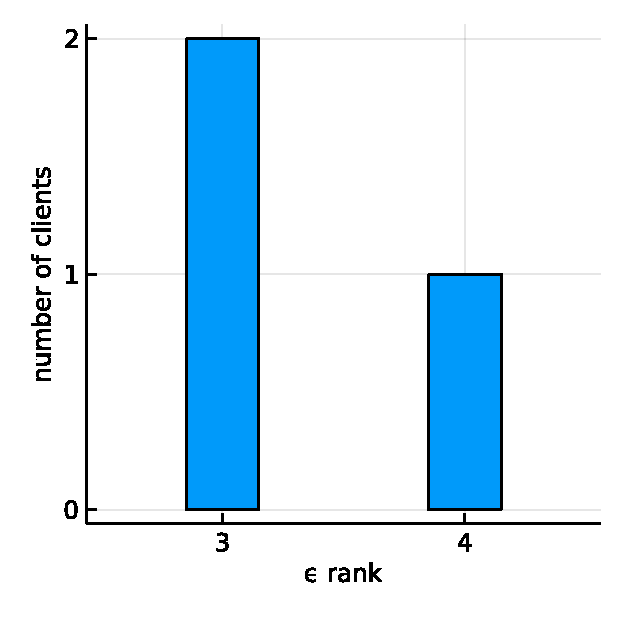
\includegraphics[width=\linewidth]{./figures/syn_embedding_matrix_adult.pdf}
      \caption{Adult dataset.}
      \label{fig:syn_embedding_matrix_adult}
    \end{subfigure}%
    \begin{subfigure}{.24\textwidth}
      \centering
      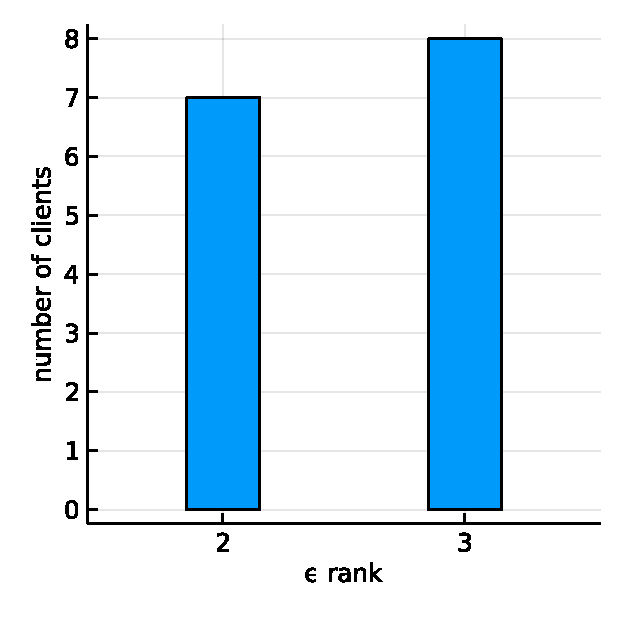
\includegraphics[width=\linewidth]{./figures/syn_embedding_matrix_web.pdf}
      \caption{Web dataset.}
      \label{fig:syn_embedding_matrix_web}
    \end{subfigure}
    \begin{subfigure}{.24\textwidth}
      \centering
      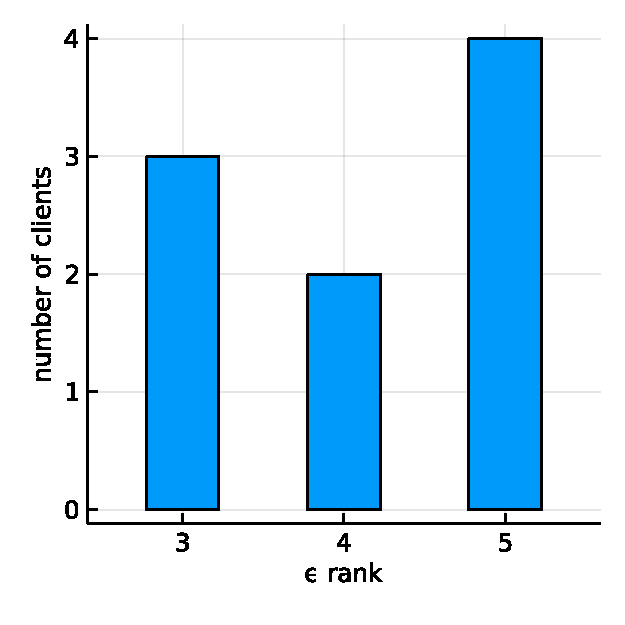
\includegraphics[width=\linewidth]{./figures/syn_embedding_matrix_covtype.pdf}
      \caption{Covtype dataset.}
      \label{fig:syn_embedding_matrix_covtype}
    \end{subfigure}
    \begin{subfigure}{.24\textwidth}
      \centering
      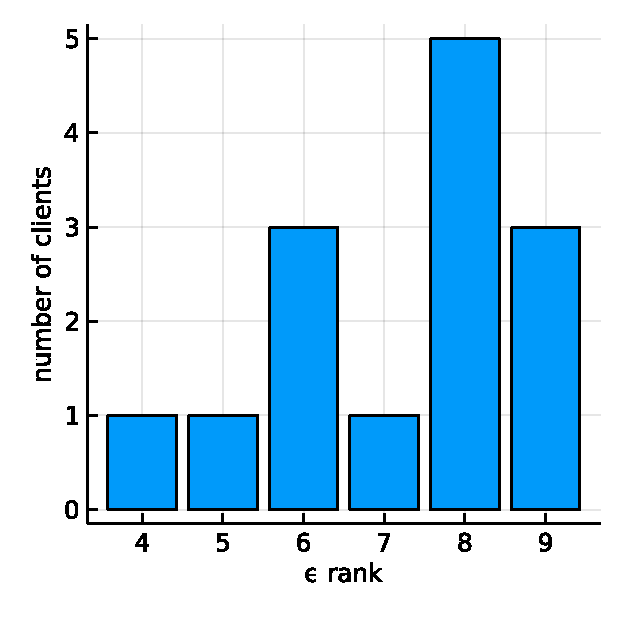
\includegraphics[width=\linewidth]{./figures/syn_embedding_matrix_rcv1.pdf}
      \caption{RCV1 dataset.}
      \label{fig:syn_embedding_matrix_rcv1}
    \end{subfigure}
    \caption{Approximated $\epsilon$-rank of embedding matrices.}
    \label{fig:syn_embedding_matrix}
\end{figure}

In this experiment, we numerically verify that the embedding matrices are approximately rank as described by Proposition~\ref{prop:low-rank}. Because we want to access the full embedding matrix, we set the batch size equal to the number of data points for all clients. The numbers of clients for the \emph{Adult}, \emph{Web}, \emph{Covtype} and \emph{RCV1} datasets are, respectively, $M = 3, 15, 9, 14$. Since computing the $\epsilon$-rank (\autoref{def:rank}) is NP-hard \cite{udell2019big}, we instead compute the rank of its truncated singular value decomposition as an approximation. More precisely, given a matrix $X \in \mathbb{R}^{m, n}$, let 
$\sigma_1 \geq \sigma_2 \geq \dots \geq \sigma_p$
be its ordered singular values, where $p = \min\{m,n\}$. Then given $\epsilon \in (0, 1)$, we define its approximated $\epsilon$-rank as 
\[\widehat \rank_\epsilon(X) = \max\{r \in [1, p] \mid \sigma_r \geq \epsilon \cdot \sigma_1\}.\]
We show a bar plot of the approximated $\epsilon$-rank of the embedding matrices in \autoref{fig:syn_embedding_matrix}, where $\epsilon=10^{-3}$, the x-axis represents the approximated $\epsilon$-rank and the y-axis represents number of clients. The plot shows that the embedding matrices have low approximated $\epsilon$-ranks for all the datasets.

\paragraph{Impact of feature heterogeneity}
\begin{figure}[t]
\begin{subfigure}{.24\textwidth}
  \centering
  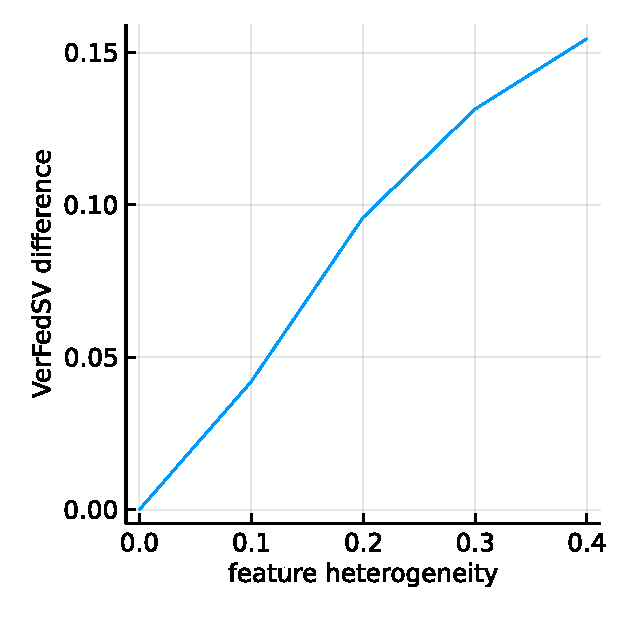
\includegraphics[width=\linewidth]{./figures/syn_similar_feature_adult.pdf}
  \caption{Adult dataset.}
  \label{fig:syn_similar_feature_adult}
\end{subfigure}%
\begin{subfigure}{.24\textwidth}
  \centering
  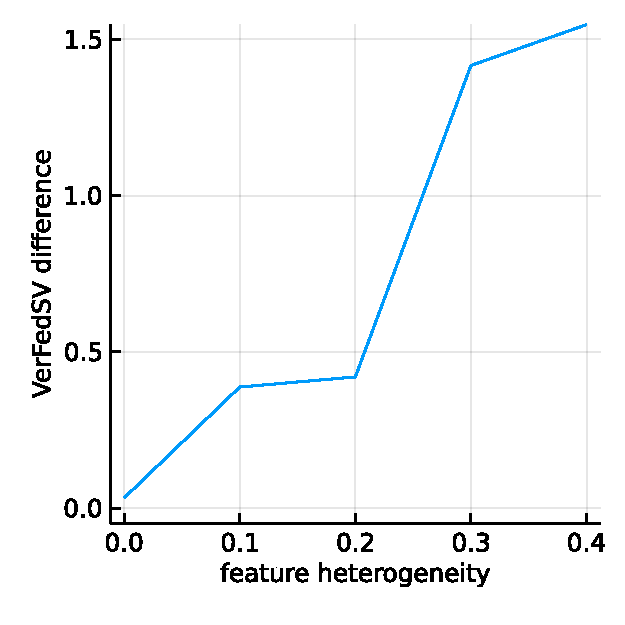
\includegraphics[width=\linewidth]{./figures/syn_similar_feature_web.pdf}
  \caption{Web dataset.}
  \label{fig:syn_similar_feature_web}
\end{subfigure} 
\begin{subfigure}{.24\textwidth}
  \centering
  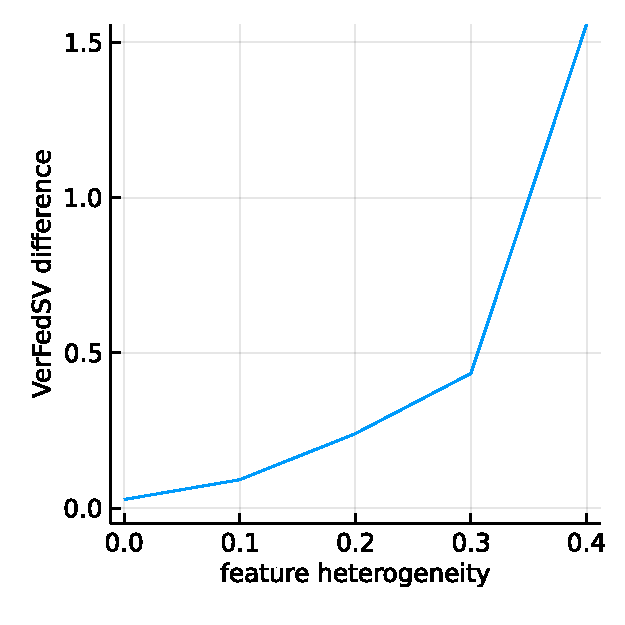
\includegraphics[width=\linewidth]{./figures/syn_similar_feature_covtype.pdf}
  \caption{Covtype dataset.}
  \label{fig:syn_similar_feature_covtype}
\end{subfigure}
\begin{subfigure}{.24\textwidth}
  \centering
  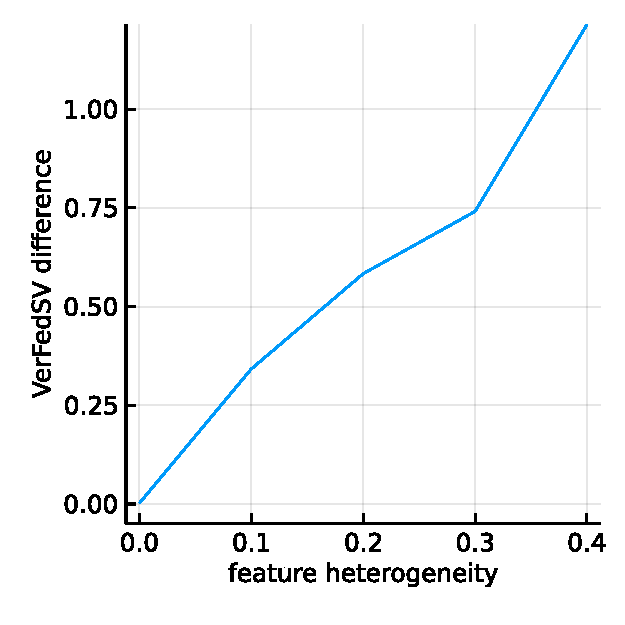
\includegraphics[width=\linewidth]{./figures/syn_similar_feature_rcv1.pdf}
  \caption{RCV1 dataset.}
  \label{fig:syn_similar_feature_rcv1}
\end{subfigure}
\caption{Relative VerFedSV difference vs feature heterogeneity.}
\label{fig:syn_similar_feature}
\end{figure}
In this experiment, we show that clients with similar features receive similar valuations under the synchronous setting. Besides the original clients, for each data set, we add 5 more clients whose features are identical to client 1 but with different level of perturbations. More precisely, for new client $i \in \{1,\dots,5\}$, we add white Gaussian noise to $(i-1)10\%$ percent of the local features, which we denote as the feature heterogeneity. Then we measure the relative difference between the original client 1 and the new clients, i.e., for any new client $i \in \{1,\dots,5\}$, let
$\texttt{diff}_i := \frac{|s - s_i|}{s}$,
where $s$ is the VerFedSV for the original client 1 and $s_i$ is the VerFedSV for the new client $i$. We show a plot of relative VerFedSV difference versus feature heterogeneity in \autoref{fig:syn_similar_feature}, where the numbers of clients for the \emph{Adult}, \emph{Web}, \emph{Covtype} and \emph{RCV1} datasets are, respectively, $M = 8, 20, 14, 19$. We can see that the relative VerFedSV difference is proportional to the feature heterogeneity. Besides, when the feature heterogeneity is equal to $0$, i.e., two clients have identical features, the relative VerFedSV difference is exactly $0$ for \emph{Adult} dataset, and is nearly $0$ for the \emph{Web}, \emph{Covtype} and \emph{RCV1} datasets, where the inexactness is due to the Monte Carlo sampling. 

\paragraph{VerFedSV for random feature}
In this experiment, we show that clients with randomly generated features receive low evaluations under synchronous setting. Besides the regular clients, for each data set, we add 5 more clients whose features are randomly generated according to different distributions. More precisely, for the new client $i \in \{1,\dots,5\}$, the features are generated from Gaussian distribution with mean equal to $i$ and variance equal to $i^2$. We show in the \autoref{tab:syn_random_feature} the percentage of the clients' VerFedSVs in the total sum of VerFedSVs, where the numbers of clients for the \emph{Adult}, \emph{Web}, \emph{Covtype} and \emph{RCV1} datasets are, respectively, $M = 8, 20, 14, 19$. As we can see from the table, regardless of the distributions, clients with randomly generated features receive much lower valuations than the regular clients for all the datasets. 
\begin{table}[t]
    \centering
    \begin{tabular}{ccccc}
    \toprule
                         & Adult & Web   & Covtype  & RCV1 \\ \midrule
     all regular clients & 99.88 & 99.73 & 97.77    & 93.84\\
     artificial client 1 & 0.01  & 0.02  & 0.39     & 1.86 \\
     artificial client 2 & 0.05  & 0.06  & 0.57     & 0.43\\
     artificial client 3 & 0.03  & 0.06  & 0.91     & 2.37\\
     artificial client 4 & 0.01  & 0.07  & 0.36     & 0.31\\
     artificial client 5 & 0.02  & 0.06  & 0.01     & 1.18\\
    \bottomrule
    \end{tabular}
    \caption{Percentage of clients' VerFedSVs in the total sum of VerFedSVs (synchronous setting).}
    \label{tab:syn_random_feature}
\end{table}

\subsection{Asynchronous Vertical Federated Learning} \label{sec:8.8.3}
In this set of experiments, we adapt VerFedSV with asynchronous VFL algorithms. We show that VerFedSV not only satisfies the fairness property under asynchronous setting (\autoref{thm:fair}), but can also reflect how frequently clients report (\autoref{prop:asyn_diff_fre}). More specifically, during the training, we let clients to communicate with server at different frequencies. For all the datasets, we asynchronously train the model for $20$ seconds and do the valuation every $0.04$ seconds, i.e., there are $T = 500$ contribution valuation time points (\autoref{def:vertical_fedsv}). 

\paragraph{Impact of communication frequency}

\begin{figure}[t]
\begin{subfigure}{.24\textwidth}
  \centering
  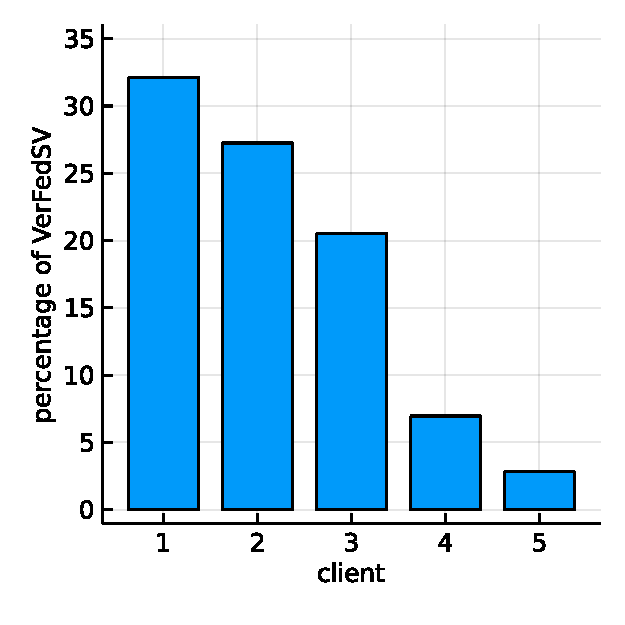
\includegraphics[width=\linewidth]{./figures/asyn_same_features_adult.pdf}
  \caption{Adult dataset.}
  \label{fig:asyn_same_feature_adult}
\end{subfigure}%
\begin{subfigure}{.24\textwidth}
  \centering
  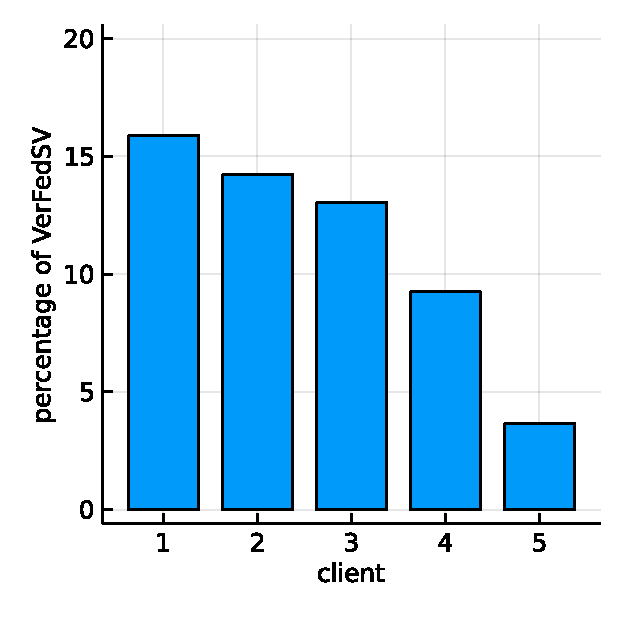
\includegraphics[width=\linewidth]{./figures/asyn_same_features_web.pdf}
  \caption{Web dataset.}
  \label{fig:asyn_same_feature_web}
\end{subfigure} 
\begin{subfigure}{.24\textwidth}
  \centering
  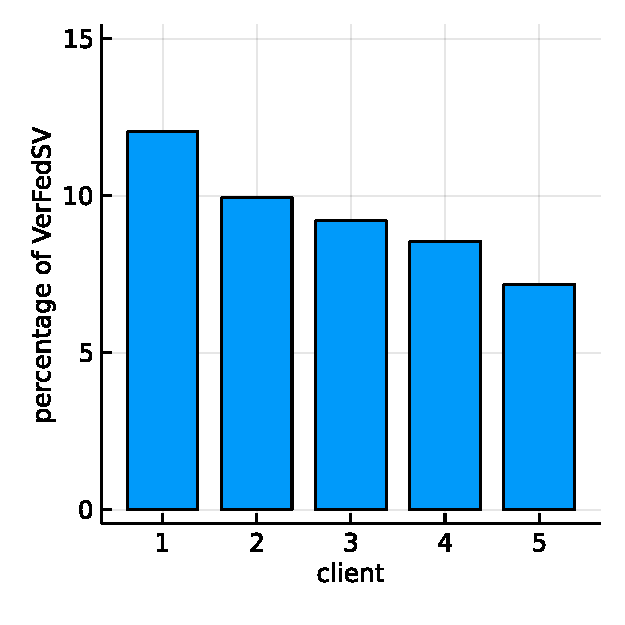
\includegraphics[width=\linewidth]{./figures/asyn_same_features_covtype.pdf}
  \caption{Covtype dataset.}
  \label{fig:asyn_same_feature_covtype}
\end{subfigure}
\begin{subfigure}{.24\textwidth}
  \centering
  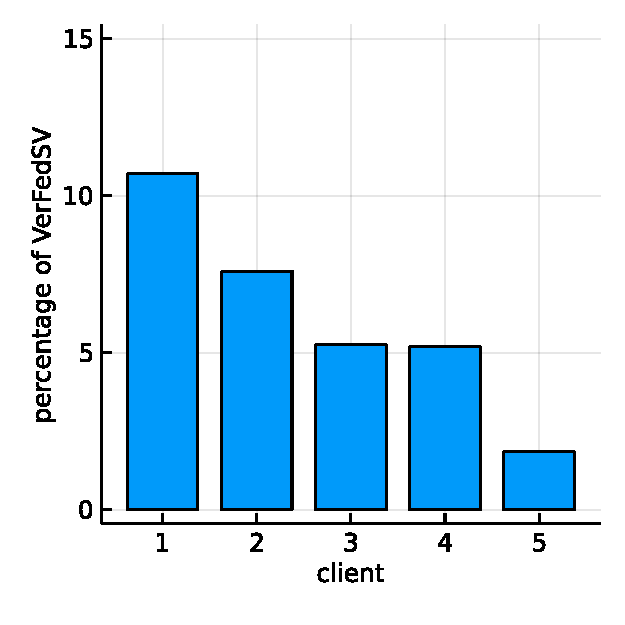
\includegraphics[width=\linewidth]{./figures/asyn_same_features_rcv1.pdf}
  \caption{RCV1 dataset.}
  \label{fig:asyn_same_feature_rcv1}
\end{subfigure}
\caption{VerFedSVs for clients with different communication frequencies.}
\label{fig:asyn_same_feature}
\end{figure}

In this experiment, we show that clients with higher communication frequency receive higher valuation. Besides the original clients, for each data set, we add 5 more clients whose features are identical to client 1 but with different level of communication frequencies. More precisely, the new client $i \in \{1,\dots,5\}$ communicates with the server every $0.01i$ seconds, i.e., the new client 1 has the highest communication frequency and the new client $5$ has the lowest. We show a plot in \autoref{fig:asyn_same_feature} of the percentage of the new clients' VerFedSVs in the total sum of VerFedSVs, where the numbers of clients for the \emph{Adult}, \emph{Web}, \emph{Covtype} and \emph{RCV1} datasets are, respectively, $M = 8, 20, 14, 19$. We can see that the percentage of VerFedSV is proportional to the communication frequency. 

\paragraph{VerFedSV for random feature}
In this experiment, we show that clients with randomly generated features receive low evaluations regardless of their communication frequencies. Besides the regular clients, for each data set, we add 5 more clients whose features are randomly generated according to standard Gaussian distribution. They have communication frequencies such that the new client $i \in \{1,\dots,5\}$ communicates with the server every $0.01i$ seconds. We show in \autoref{tab:asyn_random_feature} the percentage of the clients' VerFedSVs in the total sum of VerFedSVs, where the numbers of clients for the \emph{Adult}, \emph{Web}, \emph{Covtype} and \emph{RCV1} datasets are, respectively, $M = 8, 20, 14, 19$. Regardless of the communication frequencies, the clients with randomly generated features receive much lower valuations than the regular clients for all the datasets.
\begin{table}[t]
    \centering
    \begin{tabular}{ccccc}
    \toprule
                         & Adult & Web   & Covtype  & RCV1\\ \midrule
     all regular clients & 97.91 & 98.39 & 98.57    & 91.90\\
     artificial client 1 & 0.93  & 0.26  & 0.35     & 1.66\\
     artificial client 2 & 0.06  & 0.31  & 0.21     & 1.75\\
     artificial client 3 & 0.33  & 0.36  & 0.22     & 1.64\\
     artificial client 4 & 0.43  & 0.40  & 0.25     & 1.50\\
     artificial client 5 & 0.35  & 0.28  & 0.39     & 1.54\\
    \bottomrule
    \end{tabular}
    \caption{Percentage of clients' VerFedSVs in the total sum of VerFedSVs (asynchronous setting).}
    \label{tab:asyn_random_feature}
\end{table}

\subsection{Effectiveness of VerFedSV} \label{sec:8.8.4}
We evaluate the effectiveness of VerFedSV in both the synchronous and asynchronous VFL settings. In other words, we test whether VerFedSV can reflect the importance of clients' local features. We set all clients to have the same communication frequency to eliminate the impact of unbalanced local computational resources. We choose SHAP~\cite{lundberg2017unified} as the baseline, which is a widely-used metric for measuring feature importance in machine learning. More specifically, we first use SHAP to compute the importance scores of all the features, and then for each client, we ensemble the scores for all the local features. Note that SHAP cannot be directly used in the VFL task, as it requires access to all the local datasets and models and violates the VFL settings. So here we just use it as a reference. We use the Kendall's rank correlation (KRC)~\cite{kendall1938new} to measure the similarity between the orderings of the scores of SHAP and VerFedSV. As a by-product, we also show the similarity between the scores of VerFedSV in the synchronous and asynchronous settings. We show in \autoref{tab:comparasion_shap} the KRCs between the results of SHAP and VerFedSV, where $\corr$ denotes the KRC, $\svshap$ denotes the results from SHAP, $\svsyn$ and $\svasyn$, respectively, denote the results from VerFedSV in the synchronous and asynchronous settings, and the numbers of clients for the \emph{Adult}, \emph{Web}, \emph{Covtype} and \emph{RCV1} datasets are, respectively, set to $M = 3, 15, 9, 14$. Note that KRC returns a value in $[-1, 1]$, where ``$1$'' means two input score lists have the identical ranking and ``$-1$'' means the rankings are exactly reverted. The KRC between SHAP and VerFedSV are all greater than $0.6$. The results indicate that VerFedSV can indeed capture the feature importance well. Moreover, the KRC between $\svsyn$ and $\svasyn$ are all greater than 0.8. The results indicate that VerFedSV is consistent under both synchronous and asynchronous settings.

\begin{table}[t]
    \centering
    \begin{tabular}{ccccc}
    \toprule
                                & Adult & Web   & Covtype   & RCV1\\ \midrule
    $\corr(\svshap, \svsyn)$    & 1.0   & 0.73  & 0.94      & 0.65\\
    $\corr(\svshap, \svasyn)$   & 1.0   & 0.69  & 0.89      & 0.63\\
    $\corr(\svsyn, \svasyn)$    & 1.0   & 0.80  & 0.94      & 0.80\\
    \bottomrule
    \end{tabular}
    \caption{Kendall's rank correlation between the results of SHAP and VerFedSV's.}
    \label{tab:comparasion_shap}
\end{table}

\section{Insights} \label{sec:8.9}
In this paper, we propose a contribution valuation metric called vertical federated Shapley value (VerFedSV) for vertical federated learning (VFL). We demonstrate both theoretically and empirically that VerFedSV satisfies many desirable properties for fairness and is quite adaptable such that it can be applied under both synchronous and asynchronous VFL settings. 

There are a few interesting directions for future work.  For example, there is an interesting insight from the experiments that deserves future research.  We notice that when we keep adding clients with identical features, the total of the VerFedSV increases. This may suggest that some clients may ``cheat'' by constructing new clients with identical features so that they can receive unjustifiable rewards in the end. The issue can be resolved under the synchronous setting, for example, by checking the similarity between uploaded embeddings from clients. However, it seems there is no simple solution to resolve this issue under the asynchronous setting. 

\section{Proofs}

\subsection{Proof for Theorem 1}
\begin{proof}
    We notice that the VerFedSV can be expressed as 
    \begin{align*}
        s_m &= \frac{1}{MT}\sum_{t=1}^T\sum_{S \subseteq [M] \setminus \{m\}} \frac{1}{\binom{M-1}{|S|}} [U_t(S\cup\{m\}) - U_t(S)]\\
        &= \frac{1}{M}\sum_{S \subseteq [M] \setminus \{m\}} \frac{1}{\binom{M-1}{|S|}} \left[\frac{1}{T}\sum_{t=1}^T U_t(S\cup\{m\}) - \frac{1}{T}\sum_{t=1}^T U_t(S)\right]\\
        &= \frac{1}{M}\sum_{S \subseteq [M] \setminus \{m\}} \frac{1}{\binom{M-1}{|S|}} \left[U(S\cup\{m\}) - U(S)\right],
    \end{align*}
    which matches the expression for classical Shapley value. The result then follows. 
\end{proof}

\subsection{Proof for Proposition 1}
\begin{proof}
    It is evident that $\rank_\epsilon(\mathcal{H}^m) \leq \rank(\mathcal{H}^m) \leq d_m$ for all $m \in [M]$. So we only need to prove the remaining two upper bounds. First, we consider the difference between successive rows of the embedding matrix $\mathcal{H}^m$. For any $t \in [T-1]$ and $i \in [N]$, 
    \begin{align*}
        |\mathcal{H}^m_{t, i} - \mathcal{H}^m_{t+1, i}| &= |(h_i^m)^{(t)} - (h_i^m)^{(t+1)}|
        \\&= |\langle \theta_m^{(t)}, x^m_i\rangle - \langle \theta_m^{(t+1)}, x^m_i\rangle|
        \\&= |\langle \theta_m^{(t)} - \theta_m^{(t+1)}, x^m_i\rangle|
        \\&= \left|\langle \frac{\eta^{(t)}}{|B^{(t)}|}\sum_{j\in B^{(t)}} g_j^{(t)} x_j^m , x^m_i\rangle\right|
        \\&\leq \eta^{(t)}L.
    \end{align*}
    Thus, we obtain an upper bound on the $\rank_\epsilon(\mathcal{H}^m)$ by 
    \begin{align*}
        \rank_\epsilon(\mathcal{H}^m) &\leq \left\lceil \frac{1}{\epsilon} \sum_{t=1}^{T-1} \big\|\mathcal{H}^m[t,:] - \mathcal{H}^m[t+1, :]\big\|_{\max} \right\rceil \\
        &\leq \left\lceil \frac{L}{\epsilon} \sum_{t=1}^{T-1}\eta^{(t)} \right\rceil\\
        &\leq \left\lceil \frac{L\log(T)}{\epsilon} \right\rceil.
    \end{align*}
    Next, we consider the difference between any two columns of the embedding matrix $\mathcal{H}^m$. For any $t \in [T]$ and $i,j\in[N]$, we have 
    \begin{align*}
        |\mathcal{H}^m_{t, i} - \mathcal{H}^m_{t, j}| &= |(h_i^m)^{(t)} - (h_j^m)^{(t)}|
        \\&= |\langle \theta_m^{(t)}, x^m_i\rangle - \langle \theta_m^{(t)}, x^m_j\rangle|
        \\&\leq \|\theta_m^{(t)}\|\cdot\|x^m_i - x^m_j\|.
    \end{align*}
    It follows that 
    \[\|\mathcal{H}^m[:,i] - \mathcal{H}^m_{t, j}\|_{\max} \leq \max_{t \in [T]}\|\theta_m^{(t)}\|\cdot\|x^m_i - x^m_j\|.\]
    Let $\gamma^m = \max_{t \in [T]}\|\theta_m^{(t)}\|$ and $\mathcal{N}$ be an $\frac{\epsilon}{\gamma^m}$-net for $\{x^m_i : i \in [N]\}$. We can thus conclude that 
    \[\rank_\epsilon(\mathcal{H}^m) \leq |\mathcal{N}|.\]
    By definition of the covering number, it follows that 
    \[\rank_{\epsilon}(\mathcal{H}^m) \leq \mathcal{N}\left(\{x^m_i: i \in [N]\}, \frac{\epsilon}{\gamma^m}\right).\]
\end{proof}

\section{Proof for Proposition 2}
\begin{proof}
    Define $U,\hat U: 2^{[M]}\to\mathbb{R}$ by 
    \[U(S) := \frac{1}{T}\sum_{t=1}^T U_t(S) \quad\text{and}\quad \hat U(S) := \frac{1}{T}\sum_{t=1}^T \hat U_t(S).\]
    For any $S \subset [M]$, we know that 
    \begin{align*}
        &~|U(S) - \hat U(S)| \\
        \leq~&~\frac{1}{NT}\sum_{t=1}^T\sum_{i=1}^N \left|f\left( \sum_{m=1}^M \mathcal{H}_{t-1, i}^m; y_i\right) - f\left( \sum_{m=1}^M (w^m_{t-1})^\intercal h^m_i; y_i\right)\right| \\
        &~+ \frac{1}{NT}\sum_{t=1}^T\sum_{i=1}^N \bigg|f\left( \sum_{m\in S} \mathcal{H}_{t, i}^m + \sum_{m\notin S} \mathcal{H}_{t-1, i}^m; y_i\right) \\
        &~- f\left( \sum_{m\in S} (w^m_{t})^\intercal h^m_i + \sum_{m\notin S} (w^m_{t-1})^\intercal h^m_i; y_i\right)\bigg|\\
        \leq~&~\frac{G}{NT}\sum_{t=1}^T\sum_{i=1}^N \left|\sum_{m=1}^M \mathcal{H}_{t-1, i}^m -  \sum_{m=1}^M (w^m_{t-1})^\intercal h^m_i\right|\\
        &~+ \frac{G}{NT}\sum_{t=1}^T\sum_{i=1}^N \bigg|\left( \sum_{m\in S} \mathcal{H}_{t, i}^m + \sum_{m\notin S} \mathcal{H}_{t-1, i}^m\right) \\ 
        &~- \left( \sum_{m\in S} (w^m_{t})^\intercal h^m_i + \sum_{m\notin S} (w^m_{t-1})^\intercal h^m_i\right)\bigg| \leq GM\epsilon.
    \end{align*}
    Then we can obtain a bound on $|s_m - \hat s_m|$ by 
    \begin{align*}
        ~&~|s_m - \hat s_m| \\
        \leq ~&~ \frac{1}{M}\sum_{S \subseteq [M] \setminus \{m\}} \frac{1}{\binom{M-1}{|S|}} \left|U(S\cup\{m\}) - \hat U(S\cup\{m\})\right| + \left|U(S) - \hat U(S)\right|\\
        \leq ~&~ 2G\epsilon.
    \end{align*}
\end{proof}

\subsection{Proof for Proposition 3}
\begin{proof}
    We know that $\theta_1^*$ and $\theta_2^*$ are the optimal variables for the following convex optimization problem 
    \[\min_{\theta_1, \theta_2}\enspace \frac{1}{N}\sum_{i=1}^N f(\langle\theta_1, x_i\rangle + \langle\theta_2, x_i\rangle; y_i) = g(\theta_1 + \theta_2).\]
    Since $\theta^*$ is the unique minimizer for $g(\theta)$, it follows that $\theta_1^*$ and $\theta_2^*$ must satisfy $\theta_1^* + \theta_2^* = \theta^*$. Denote $d_1^{(t)}$ as the update for $\theta_1$ at the $t$th iteration and $d_2^{(t)}$ as the update for for $\theta_2$ at the $t$th iteration. By the construction, we know that 
    \[\mathbb{E} \left[ \sum_{t=1}^\infty ( d_1^{(t)} + d_2^{(t)} ) \right] = \theta^* \enspace\text{and}\enspace \mathbb{E}\left[ \sum_{t=1}^\infty d_2^{(t)} \right] = \rho \mathbb{E}\left[ \sum_{t=1}^\infty d_1^{(t)} \right].\]
    Therefore
    \[
        \mathbb{E}[\theta_1^*] = \mathbb{E}\left[ \sum_{t=1}^\infty d_1^{(t)} \right] = \frac{1}{1+\rho} \theta^* \enspace\text{and}\enspace \mathbb{E}[\theta_2^*] = \mathbb{E}\left[ \sum_{t=1}^\infty d_2^{(t)} \right] = \frac{\rho}{1+\rho} \theta^*.
    \]
    Now we consider VerFedSV. By the definition, we have 
    \[\mathbb{E}[s_1 - s_2] = 2\left[g\left(\frac{\rho}{1+\rho}\theta^*\right) - g\left(\frac{1}{1+\rho}\theta^*\right)\right].\]
    Define $h:[0,1]\to\mathbb{R}$ as $h(\lambda) = g(\lambda \theta^*)$. Since $g$ is $\mu$-strongly convex and $\theta^*$ is the unique minimizer, it follows that $h$ is $\mu\|\theta^*\|^2$-strongly convex and is monotonically non-increasing on $[0,1]$. Thus, we can conclude that 
    \[\mathbb{E}[s_1] \geq \mathbb{E}[s_2] + 2\left[h\left(\frac{\rho}{1+\rho}\right) - h\left(\frac{1}{1+\rho}\right)\right] \geq \mathbb{E}[s_2] + \mu\left(\frac{1-\rho}{1+\rho}\right)^2\|\theta^*\|^2.\]
\end{proof}

\part{Paths forward}

%    9. Conclusion and future work

%% The following is a directive for TeXShop to indicate the main file
%%!TEX root = diss.tex
\chapter{Conclusion and future work}
\label{ch:conclusion}

The primary contribution of this dissertation consists of three parts: structured optimization, federated optimization, and applications of structured optimization in federated learning, where the key innovation is the usage and extension of modern duality theory. We review some of the results from this thesis and propose potential next paths in this chapter.


\section{Structured optimization}

In \autoref{ch:Dual-Struc-Opt}, we developed the polar alignment property characterizing the duality correspondence in structured optimization. As shown in \autoref{ch:App-Sig-Demix}, \autoref{ch:App-Primal-Retrieval} and \autoref{ch:App-AtomicOpt}, the polar alignment property allows us to design new models and develop efficient algorithms for structured optimization. Further research opportunities remain. For example, most (if not all) of the
ideas we have presented could be generalized to the infinite-dimensional
setting, which would accommodate more general decompositions. Also, other
standard algorithms, such as splitting and bundle methods~\cite{fan2019bundle}, seem to exhibit properties that can easily be explained using the language of polar alignment.

In \autoref{ch:App-Sig-Demix}, we develop a two-stage approach for deconvolving a superposition of mutiple structural signals into its constituent components. There are opportunities for future research. As we have demonstrated, the random rotation model is a useful mechanism for introducing incoherence among the individual signals. However, even in contexts where it's possible to rotate the signals, it may prove too costly to do so in practice because the rotations need to be applied at each iteration of the algorithm in \autoref{ch:App-AtomicOpt}. We might then consider other mechanisms for introducing incoherence that are computationally cheaper, and rely instead, for example, on some fast random transform. The literature on demixing abounds with various incoherence notions. We wish to explore what is the relationship between these and definition of $\beta$-incoherence that we adopt. Alternative incoherence definitions may prove useful in deriving other mechanisms for inducing incoherence in the signals. Moreover, a significant assumption of our analysis is that the parameters $\lambda_i$ exactly equilibrate the gauge values for each signal. In practice, there are many cases where the parameters $\lambda_i$ are known. For example, in some secure communication problems~\citep[Section~1.3.1]{mccoy2014sharp}, the sender can normalize the signals before mixing them. On the other hand, when the parameters $\lambda_i$ are not known, we can apply a grid search to obtain reasonable approximations. It may be possible to analyze how the stability in the recovery of the signals depends on errors that might exist in the ideal parameter choices.

In \autoref{ch:App-Primal-Retrieval}, we develop a primal-retrieval strategy for structured optimization. Further research opportunities remain, particularly for designing meaningful primal-retrieval strategy for non-polyhedral and non-spectral atomic sets. Moreover, the primal-retrieval technique we developed is algorithm-agnostic, it is possible to develop more efficient primal-retrieval rule that associated with specific optimization algorithms such as the conditional-gradient method.

In \autoref{ch:App-AtomicOpt}, we introduce our open-source Julia package \texttt{AtomicOpt.jl} for solving structured optimization problems. There are at least two possible opportunities to improve this package: adding more dual-based candidate algorithms besides the ones introduced in \autoref{sec:5-2}, and adding more basic atomic sets besides the ones introduced in \autoref{sec:5-3}. 

\section{Federated optimization}

In \autoref{ch:Dual-Struc-Opt}, by tackling the dual problem of federated optimization, we propose the federated dual coordinate descent (FedDCD) algorithm and its variants. More importantly, FedDCD provides a general framework for federated optimization and suggests many interesting future research directions. First, it is possible to develop an asynchronous version of FedDCD by leveraging well-studied analysis of asynchronous parallel coordinate descent methods~\citep{LiuW15,0002WRBS15}. Next, one might consider client sampling strategies other than the standard uniform sampling. For example, there are some recent studies of the coordinate descent with the greedy selection rule~\citep{NutiniSLFK15,BCD_julie,fang2020greed}, which can be adopted with FedDCD. Finally, the lower bound of complexity of first-order methods with random participation for federated optimization is still an open problem. As we have shown in \autoref{sec:lowerBound}, our lower bound analysis has a $\BigOh(\sqrt{N})$ gap to the upper bound of accelerated FedDCD. We hope to explore whether the lower bound can be further tightened or an algorithm with a faster convergence rate can be developed. 


\section{Applications of structured optimization in federated learning}

In \autoref{ch:Val-HFL} and \autoref{ch:Val-VFL}, we develop contribution valuation strategies ComFedSv and VerFedSV, respectively for, horizontal federated learning and vertical federated learning.  Our study advances the frontier in this emerging important direction. There are also many interesting future directions. For example, under the framework of federated learning, there may exist some other properties needed for fairness in federated learning in addition to those in the Shapley fairness. As another example, we otice that when we keep adding clients with identical features, the total of the VerFedSV increases. This may suggest that some clients may ``cheat'' by constructing new clients with identical features so that they can receive unjustifiable rewards in the end. The issue can be resolved under the synchronous setting, for example, by checking the similarity between uploaded embeddings from clients. However, it seems there is no simple solution to resolve this issue under the asynchronous setting. 


%    10. Bibliography
\begin{singlespace}
\raggedright
\bibliographystyle{plainnat}
\bibliography{biblio}
\end{singlespace}

\backmatter



\end{document}
